\documentclass[twoside]{book}

% Packages required by doxygen
\usepackage{fixltx2e}
\usepackage{calc}
\usepackage{doxygen}
\usepackage[export]{adjustbox} % also loads graphicx
\usepackage{graphicx}
\usepackage[utf8]{inputenc}
\usepackage{makeidx}
\usepackage{multicol}
\usepackage{multirow}
\PassOptionsToPackage{warn}{textcomp}
\usepackage{textcomp}
\usepackage[nointegrals]{wasysym}
\usepackage[table]{xcolor}

% Font selection
\usepackage[T1]{fontenc}
\usepackage[scaled=.90]{helvet}
\usepackage{courier}
\usepackage{amssymb}
\usepackage{sectsty}
\renewcommand{\familydefault}{\sfdefault}
\allsectionsfont{%
  \fontseries{bc}\selectfont%
  \color{darkgray}%
}
\renewcommand{\DoxyLabelFont}{%
  \fontseries{bc}\selectfont%
  \color{darkgray}%
}
\newcommand{\+}{\discretionary{\mbox{\scriptsize$\hookleftarrow$}}{}{}}

% Page & text layout
\usepackage{geometry}
\geometry{%
  a4paper,%
  top=2.5cm,%
  bottom=2.5cm,%
  left=2.5cm,%
  right=2.5cm%
}
\tolerance=750
\hfuzz=15pt
\hbadness=750
\setlength{\emergencystretch}{15pt}
\setlength{\parindent}{0cm}
\setlength{\parskip}{3ex plus 2ex minus 2ex}
\makeatletter
\renewcommand{\paragraph}{%
  \@startsection{paragraph}{4}{0ex}{-1.0ex}{1.0ex}{%
    \normalfont\normalsize\bfseries\SS@parafont%
  }%
}
\renewcommand{\subparagraph}{%
  \@startsection{subparagraph}{5}{0ex}{-1.0ex}{1.0ex}{%
    \normalfont\normalsize\bfseries\SS@subparafont%
  }%
}
\makeatother

% Headers & footers
\usepackage{fancyhdr}
\pagestyle{fancyplain}
\fancyhead[LE]{\fancyplain{}{\bfseries\thepage}}
\fancyhead[CE]{\fancyplain{}{}}
\fancyhead[RE]{\fancyplain{}{\bfseries\leftmark}}
\fancyhead[LO]{\fancyplain{}{\bfseries\rightmark}}
\fancyhead[CO]{\fancyplain{}{}}
\fancyhead[RO]{\fancyplain{}{\bfseries\thepage}}
\fancyfoot[LE]{\fancyplain{}{}}
\fancyfoot[CE]{\fancyplain{}{}}
\fancyfoot[RE]{\fancyplain{}{\bfseries\scriptsize Generated by Doxygen }}
\fancyfoot[LO]{\fancyplain{}{\bfseries\scriptsize Generated by Doxygen }}
\fancyfoot[CO]{\fancyplain{}{}}
\fancyfoot[RO]{\fancyplain{}{}}
\renewcommand{\footrulewidth}{0.4pt}
\renewcommand{\chaptermark}[1]{%
  \markboth{#1}{}%
}
\renewcommand{\sectionmark}[1]{%
  \markright{\thesection\ #1}%
}

% Indices & bibliography
\usepackage{natbib}
\usepackage[titles]{tocloft}
\setcounter{tocdepth}{3}
\setcounter{secnumdepth}{5}
\makeindex

% Hyperlinks (required, but should be loaded last)
\usepackage{ifpdf}
\ifpdf
  \usepackage[pdftex,pagebackref=true]{hyperref}
\else
  \usepackage[ps2pdf,pagebackref=true]{hyperref}
\fi
\hypersetup{%
  colorlinks=true,%
  linkcolor=blue,%
  citecolor=blue,%
  unicode%
}

% Custom commands
\newcommand{\clearemptydoublepage}{%
  \newpage{\pagestyle{empty}\cleardoublepage}%
}

\usepackage{caption}
\captionsetup{labelsep=space,justification=centering,font={bf},singlelinecheck=off,skip=4pt,position=top}

%===== C O N T E N T S =====

\begin{document}

% Titlepage & ToC
\hypersetup{pageanchor=false,
             bookmarksnumbered=true,
             pdfencoding=unicode
            }
\pagenumbering{roman}
\begin{titlepage}
\vspace*{7cm}
\begin{center}%
{\Large Variational Analysis }\\
\vspace*{1cm}
{\large Generated by Doxygen 1.8.11}\\
\end{center}
\end{titlepage}
\clearemptydoublepage
\tableofcontents
\clearemptydoublepage
\pagenumbering{arabic}
\hypersetup{pageanchor=true}

%--- Begin generated contents ---
\chapter{Modules Index}
\section{Modules List}
Here is a list of all modules with brief descriptions\+:\begin{DoxyCompactList}
\item\contentsline{section}{\hyperlink{namespaceconstants}{constants} }{\pageref{namespaceconstants}}{}
\item\contentsline{section}{\hyperlink{namespaceio}{io} }{\pageref{namespaceio}}{}
\item\contentsline{section}{\hyperlink{namespacelu}{lu} }{\pageref{namespacelu}}{}
\item\contentsline{section}{\hyperlink{namespacenumerics}{numerics} }{\pageref{namespacenumerics}}{}
\item\contentsline{section}{\hyperlink{namespacephysics}{physics} }{\pageref{namespacephysics}}{}
\item\contentsline{section}{\hyperlink{namespaceportable}{portable} }{\pageref{namespaceportable}}{}
\item\contentsline{section}{\hyperlink{namespacesettings}{settings} }{\pageref{namespacesettings}}{}
\item\contentsline{section}{\hyperlink{namespacesetup}{setup} }{\pageref{namespacesetup}}{}
\item\contentsline{section}{\hyperlink{namespacetime}{time} }{\pageref{namespacetime}}{}
\end{DoxyCompactList}

\chapter{File Index}
\section{File List}
Here is a list of all files with brief descriptions\+:\begin{DoxyCompactList}
\item\contentsline{section}{/home/unimelb.\+edu.\+au/mbergemann/va\+\_\+analysis/src/\hyperlink{2d__put_8f90}{2d\+\_\+put.\+f90} }{\pageref{2d__put_8f90}}{}
\item\contentsline{section}{/home/unimelb.\+edu.\+au/mbergemann/va\+\_\+analysis/src/\hyperlink{3d__put_8f90}{3d\+\_\+put.\+f90} }{\pageref{3d__put_8f90}}{}
\item\contentsline{section}{/home/unimelb.\+edu.\+au/mbergemann/va\+\_\+analysis/src/\hyperlink{budget__put_8f90}{budget\+\_\+put.\+f90} }{\pageref{budget__put_8f90}}{}
\item\contentsline{section}{/home/unimelb.\+edu.\+au/mbergemann/va\+\_\+analysis/src/\hyperlink{constants_8f90}{constants.\+f90} }{\pageref{constants_8f90}}{}
\item\contentsline{section}{/home/unimelb.\+edu.\+au/mbergemann/va\+\_\+analysis/src/\hyperlink{io_8f90}{io.\+f90} }{\pageref{io_8f90}}{}
\item\contentsline{section}{/home/unimelb.\+edu.\+au/mbergemann/va\+\_\+analysis/src/\hyperlink{lu_8f90}{lu.\+f90} }{\pageref{lu_8f90}}{}
\item\contentsline{section}{/home/unimelb.\+edu.\+au/mbergemann/va\+\_\+analysis/src/\hyperlink{numerics_8f90}{numerics.\+f90} }{\pageref{numerics_8f90}}{}
\item\contentsline{section}{/home/unimelb.\+edu.\+au/mbergemann/va\+\_\+analysis/src/\hyperlink{physics_8f90}{physics.\+f90} }{\pageref{physics_8f90}}{}
\item\contentsline{section}{/home/unimelb.\+edu.\+au/mbergemann/va\+\_\+analysis/src/\hyperlink{portable_8f90}{portable.\+f90} }{\pageref{portable_8f90}}{}
\item\contentsline{section}{/home/unimelb.\+edu.\+au/mbergemann/va\+\_\+analysis/src/\hyperlink{process__va__output_8f90}{process\+\_\+va\+\_\+output.\+f90} }{\pageref{process__va__output_8f90}}{}
\item\contentsline{section}{/home/unimelb.\+edu.\+au/mbergemann/va\+\_\+analysis/src/\hyperlink{settings_8f90}{settings.\+f90} }{\pageref{settings_8f90}}{}
\item\contentsline{section}{/home/unimelb.\+edu.\+au/mbergemann/va\+\_\+analysis/src/\hyperlink{setup_8py}{setup.\+py} }{\pageref{setup_8py}}{}
\item\contentsline{section}{/home/unimelb.\+edu.\+au/mbergemann/va\+\_\+analysis/src/\hyperlink{time_8f90}{time.\+f90} }{\pageref{time_8f90}}{}
\item\contentsline{section}{/home/unimelb.\+edu.\+au/mbergemann/va\+\_\+analysis/src/\hyperlink{variational__analysis_8f90}{variational\+\_\+analysis.\+f90} }{\pageref{variational__analysis_8f90}}{}
\end{DoxyCompactList}

\chapter{Module Documentation}
\hypertarget{namespaceconstants}{}\section{constants Module Reference}
\label{namespaceconstants}\index{constants@{constants}}
\subsection*{Variables}
\begin{DoxyCompactItemize}
\item 
real(kind=rk8), parameter \hyperlink{namespaceconstants_a064bd715409f723a4e6d45b6300c5ca0}{pi} = 3.\+14159265
\item 
real(kind=rk8), parameter \hyperlink{namespaceconstants_afaa5eaa2c9ee648a808fb8e1c94e76f8}{rearth} = 6371000
\item 
real(kind=rk8), parameter \hyperlink{namespaceconstants_a67051296d7b4bcd0d4cee08bba6e46fa}{omega} = 7.\+292\+E-\/05
\item 
real(kind=rk8), parameter \hyperlink{namespaceconstants_ad91564da82b97ea0d29ce0565565db85}{rd} = 287.\+04
\item 
real(kind=rk8), parameter \hyperlink{namespaceconstants_a7ef8fc37397fbfbefd3c22883378dcc5}{rw} = 461.\+50
\item 
real(kind=rk8), parameter \hyperlink{namespaceconstants_a046aef138fbc8d05251d4fdc6eb3ee89}{g} = 9.\+8
\item 
real(kind=rk8), parameter \hyperlink{namespaceconstants_afb3befdfd57058ee9d073b832134a601}{lv0} = 2.\+5\+E6
\item 
real(kind=rk8), parameter \hyperlink{namespaceconstants_ab8db38b502faac0658c66b0d0b56c266}{lv} = 2.\+501\+E6
\item 
real(kind=rk8), parameter \hyperlink{namespaceconstants_a0fdb1c80757efccb4c694c79206a3d83}{ls} = 2.\+834\+E6
\item 
real(kind=rk8), parameter \hyperlink{namespaceconstants_abf3a57ecb3de0f79c3155c170db798f6}{ls1} = 2.\+834\+E6
\item 
real(kind=rk8), parameter \hyperlink{namespaceconstants_a32354adf3493f59d0fc17b0302b2c368}{cpd} = 1005.\+7
\item 
real(kind=rk8), parameter \hyperlink{namespaceconstants_afc5ea9cd5f9cf3a42e750ba5ab73c967}{cpv} = 1870.\+0
\item 
real(kind=rk8), parameter \hyperlink{namespaceconstants_a4f2911e99beba65b9371b9a80d7c08d0}{cl} = 4190.\+0
\item 
real(kind=rk8), parameter \hyperlink{namespaceconstants_a753fbbdd5d5b4af00d6819cb78ba99a1}{t0} = 273.\+15
\item 
real(kind=rk8), parameter \hyperlink{namespaceconstants_a84ecaaf3771cbbfe65f7b15ef26bee36}{cd} = 3.\+0\+E-\/3
\end{DoxyCompactItemize}


\subsection{Variable Documentation}
\index{constants@{constants}!cd@{cd}}
\index{cd@{cd}!constants@{constants}}
\subsubsection[{\texorpdfstring{cd}{cd}}]{\setlength{\rightskip}{0pt plus 5cm}real (kind=rk8), parameter constants\+::cd = 3.\+0\+E-\/3}\hypertarget{namespaceconstants_a84ecaaf3771cbbfe65f7b15ef26bee36}{}\label{namespaceconstants_a84ecaaf3771cbbfe65f7b15ef26bee36}


Definition at line 25 of file constants.\+f90.


\begin{DoxyCode}
25 \textcolor{keywordtype}{REAL (KIND=RK8)}, \textcolor{keywordtype}{PARAMETER}  :: cd       = 3.0e-3            \textcolor{comment}{! Skin friction coefficient.}
\end{DoxyCode}
\index{constants@{constants}!cl@{cl}}
\index{cl@{cl}!constants@{constants}}
\subsubsection[{\texorpdfstring{cl}{cl}}]{\setlength{\rightskip}{0pt plus 5cm}real (kind=rk8), parameter constants\+::cl = 4190.\+0}\hypertarget{namespaceconstants_a4f2911e99beba65b9371b9a80d7c08d0}{}\label{namespaceconstants_a4f2911e99beba65b9371b9a80d7c08d0}


Definition at line 23 of file constants.\+f90.


\begin{DoxyCode}
23 \textcolor{keywordtype}{REAL (KIND=RK8)}, \textcolor{keywordtype}{PARAMETER}  :: cl       = 4190.0            \textcolor{comment}{! Specific heat capcity of liquid water
       (J/kg/K)}
\end{DoxyCode}
\index{constants@{constants}!cpd@{cpd}}
\index{cpd@{cpd}!constants@{constants}}
\subsubsection[{\texorpdfstring{cpd}{cpd}}]{\setlength{\rightskip}{0pt plus 5cm}real (kind=rk8), parameter constants\+::cpd = 1005.\+7}\hypertarget{namespaceconstants_a32354adf3493f59d0fc17b0302b2c368}{}\label{namespaceconstants_a32354adf3493f59d0fc17b0302b2c368}


Definition at line 21 of file constants.\+f90.


\begin{DoxyCode}
21 \textcolor{keywordtype}{REAL (KIND=RK8)}, \textcolor{keywordtype}{PARAMETER}  :: cpd      = 1005.7            \textcolor{comment}{! Heat capacity of dry air at constant pressure
       (J/kg/K)}
\end{DoxyCode}
\index{constants@{constants}!cpv@{cpv}}
\index{cpv@{cpv}!constants@{constants}}
\subsubsection[{\texorpdfstring{cpv}{cpv}}]{\setlength{\rightskip}{0pt plus 5cm}real (kind=rk8), parameter constants\+::cpv = 1870.\+0}\hypertarget{namespaceconstants_afc5ea9cd5f9cf3a42e750ba5ab73c967}{}\label{namespaceconstants_afc5ea9cd5f9cf3a42e750ba5ab73c967}


Definition at line 22 of file constants.\+f90.


\begin{DoxyCode}
22 \textcolor{keywordtype}{REAL (KIND=RK8)}, \textcolor{keywordtype}{PARAMETER}  :: cpv      = 1870.0            \textcolor{comment}{! Heat capacity of water vapour at constant
       pressure (J/kg/K)}
\end{DoxyCode}
\index{constants@{constants}!g@{g}}
\index{g@{g}!constants@{constants}}
\subsubsection[{\texorpdfstring{g}{g}}]{\setlength{\rightskip}{0pt plus 5cm}real (kind=rk8), parameter constants\+::g = 9.\+8}\hypertarget{namespaceconstants_a046aef138fbc8d05251d4fdc6eb3ee89}{}\label{namespaceconstants_a046aef138fbc8d05251d4fdc6eb3ee89}


Definition at line 16 of file constants.\+f90.


\begin{DoxyCode}
16 \textcolor{keywordtype}{REAL (KIND=RK8)}, \textcolor{keywordtype}{PARAMETER}  :: g        = 9.8               \textcolor{comment}{! Gravitational acceleration, at Earth's
       surface (m/s^2)}
\end{DoxyCode}
\index{constants@{constants}!ls@{ls}}
\index{ls@{ls}!constants@{constants}}
\subsubsection[{\texorpdfstring{ls}{ls}}]{\setlength{\rightskip}{0pt plus 5cm}real (kind=rk8), parameter constants\+::ls = 2.\+834\+E6}\hypertarget{namespaceconstants_a0fdb1c80757efccb4c694c79206a3d83}{}\label{namespaceconstants_a0fdb1c80757efccb4c694c79206a3d83}


Definition at line 19 of file constants.\+f90.


\begin{DoxyCode}
19 \textcolor{keywordtype}{REAL (KIND=RK8)}, \textcolor{keywordtype}{PARAMETER}  :: ls       = 2.834e6
\end{DoxyCode}
\index{constants@{constants}!ls1@{ls1}}
\index{ls1@{ls1}!constants@{constants}}
\subsubsection[{\texorpdfstring{ls1}{ls1}}]{\setlength{\rightskip}{0pt plus 5cm}real (kind=rk8), parameter constants\+::ls1 = 2.\+834\+E6}\hypertarget{namespaceconstants_abf3a57ecb3de0f79c3155c170db798f6}{}\label{namespaceconstants_abf3a57ecb3de0f79c3155c170db798f6}


Definition at line 20 of file constants.\+f90.


\begin{DoxyCode}
20 \textcolor{keywordtype}{REAL (KIND=RK8)}, \textcolor{keywordtype}{PARAMETER}  :: ls1      = 2.834e6
\end{DoxyCode}
\index{constants@{constants}!lv@{lv}}
\index{lv@{lv}!constants@{constants}}
\subsubsection[{\texorpdfstring{lv}{lv}}]{\setlength{\rightskip}{0pt plus 5cm}real (kind=rk8), parameter constants\+::lv = 2.\+501\+E6}\hypertarget{namespaceconstants_ab8db38b502faac0658c66b0d0b56c266}{}\label{namespaceconstants_ab8db38b502faac0658c66b0d0b56c266}


Definition at line 18 of file constants.\+f90.


\begin{DoxyCode}
18 \textcolor{keywordtype}{REAL (KIND=RK8)}, \textcolor{keywordtype}{PARAMETER}  :: lv       = 2.501e6
\end{DoxyCode}
\index{constants@{constants}!lv0@{lv0}}
\index{lv0@{lv0}!constants@{constants}}
\subsubsection[{\texorpdfstring{lv0}{lv0}}]{\setlength{\rightskip}{0pt plus 5cm}real (kind=rk8), parameter constants\+::lv0 = 2.\+5\+E6}\hypertarget{namespaceconstants_afb3befdfd57058ee9d073b832134a601}{}\label{namespaceconstants_afb3befdfd57058ee9d073b832134a601}


Definition at line 17 of file constants.\+f90.


\begin{DoxyCode}
17 \textcolor{keywordtype}{REAL (KIND=RK8)}, \textcolor{keywordtype}{PARAMETER}  :: lv0      = 2.5e6
\end{DoxyCode}
\index{constants@{constants}!omega@{omega}}
\index{omega@{omega}!constants@{constants}}
\subsubsection[{\texorpdfstring{omega}{omega}}]{\setlength{\rightskip}{0pt plus 5cm}real (kind=rk8), parameter constants\+::omega = 7.\+292\+E-\/05}\hypertarget{namespaceconstants_a67051296d7b4bcd0d4cee08bba6e46fa}{}\label{namespaceconstants_a67051296d7b4bcd0d4cee08bba6e46fa}


Definition at line 13 of file constants.\+f90.


\begin{DoxyCode}
13 \textcolor{keywordtype}{REAL (KIND=RK8)}, \textcolor{keywordtype}{PARAMETER}  :: omega    = 7.292e-05         \textcolor{comment}{! Rotational rate of Earth (rad/s) (note: 1
       rev/sidereal day)}
\end{DoxyCode}
\index{constants@{constants}!pi@{pi}}
\index{pi@{pi}!constants@{constants}}
\subsubsection[{\texorpdfstring{pi}{pi}}]{\setlength{\rightskip}{0pt plus 5cm}real (kind=rk8), parameter constants\+::pi = 3.\+14159265}\hypertarget{namespaceconstants_a064bd715409f723a4e6d45b6300c5ca0}{}\label{namespaceconstants_a064bd715409f723a4e6d45b6300c5ca0}


Definition at line 11 of file constants.\+f90.


\begin{DoxyCode}
11 \textcolor{keywordtype}{REAL (KIND=RK8)}, \textcolor{keywordtype}{PARAMETER}  :: pi       = 3.14159265
\end{DoxyCode}
\index{constants@{constants}!rd@{rd}}
\index{rd@{rd}!constants@{constants}}
\subsubsection[{\texorpdfstring{rd}{rd}}]{\setlength{\rightskip}{0pt plus 5cm}real (kind=rk8), parameter constants\+::rd = 287.\+04}\hypertarget{namespaceconstants_ad91564da82b97ea0d29ce0565565db85}{}\label{namespaceconstants_ad91564da82b97ea0d29ce0565565db85}


Definition at line 14 of file constants.\+f90.


\begin{DoxyCode}
14 \textcolor{keywordtype}{REAL (KIND=RK8)}, \textcolor{keywordtype}{PARAMETER}  :: rd       = 287.04            \textcolor{comment}{! Gas constant for dry air.}
\end{DoxyCode}
\index{constants@{constants}!rearth@{rearth}}
\index{rearth@{rearth}!constants@{constants}}
\subsubsection[{\texorpdfstring{rearth}{rearth}}]{\setlength{\rightskip}{0pt plus 5cm}real (kind=rk8), parameter constants\+::rearth = 6371000}\hypertarget{namespaceconstants_afaa5eaa2c9ee648a808fb8e1c94e76f8}{}\label{namespaceconstants_afaa5eaa2c9ee648a808fb8e1c94e76f8}


Definition at line 12 of file constants.\+f90.


\begin{DoxyCode}
12 \textcolor{keywordtype}{REAL (KIND=RK8)}, \textcolor{keywordtype}{PARAMETER}  :: rearth   = 6371000           \textcolor{comment}{! Radius of the Earth, in metres.}
\end{DoxyCode}
\index{constants@{constants}!rw@{rw}}
\index{rw@{rw}!constants@{constants}}
\subsubsection[{\texorpdfstring{rw}{rw}}]{\setlength{\rightskip}{0pt plus 5cm}real (kind=rk8), parameter constants\+::rw = 461.\+50}\hypertarget{namespaceconstants_a7ef8fc37397fbfbefd3c22883378dcc5}{}\label{namespaceconstants_a7ef8fc37397fbfbefd3c22883378dcc5}


Definition at line 15 of file constants.\+f90.


\begin{DoxyCode}
15 \textcolor{keywordtype}{REAL (KIND=RK8)}, \textcolor{keywordtype}{PARAMETER}  :: rw       = 461.50            \textcolor{comment}{! Gas constant for saturated air.}
\end{DoxyCode}
\index{constants@{constants}!t0@{t0}}
\index{t0@{t0}!constants@{constants}}
\subsubsection[{\texorpdfstring{t0}{t0}}]{\setlength{\rightskip}{0pt plus 5cm}real (kind=rk8), parameter constants\+::t0 = 273.\+15}\hypertarget{namespaceconstants_a753fbbdd5d5b4af00d6819cb78ba99a1}{}\label{namespaceconstants_a753fbbdd5d5b4af00d6819cb78ba99a1}


Definition at line 24 of file constants.\+f90.


\begin{DoxyCode}
24 \textcolor{keywordtype}{REAL (KIND=RK8)}, \textcolor{keywordtype}{PARAMETER}  :: t0       = 273.15            \textcolor{comment}{! Temperature in Kelvin of 0 Celsius. (K)}
\end{DoxyCode}

\hypertarget{namespaceio}{}\section{io Module Reference}
\label{namespaceio}\index{io@{io}}
\subsection*{Functions/\+Subroutines}
\begin{DoxyCompactItemize}
\item 
subroutine \hyperlink{namespaceio_abed61f2af0a37265b7a1d15300f61996}{ipt\+\_\+vht} (I\+N\+P\+U\+T\+F\+I\+LE, I\+N\+S\+T\+R\+U\+M\+E\+NT, NV, NP, N\+ST, NT, V, P, ST, T, D)
\item 
subroutine \hyperlink{namespaceio_ae478b0148dea487c688bfea00e08cade}{ipt\+\_\+ht} (I\+N\+P\+U\+T\+F\+I\+LE, I\+N\+S\+T\+R\+U\+M\+E\+NT, NV, N\+ST, NT, V, ST, L\+ON, L\+AT, T, D)
\item 
subroutine \hyperlink{namespaceio_a1feb605e982e6696d29a63e635b8d3e1}{opt\+\_\+vht\+\_\+netcdf} (O\+U\+T\+P\+U\+T\+F\+I\+LE, I\+N\+S\+T\+R\+U\+M\+E\+NT, NV, NP, N\+ST, NT, V, P, ST, T, D)
\item 
subroutine \hyperlink{namespaceio_a63d1618c60598d1e5ac65348efb74bdc}{opt\+\_\+3d\+\_\+netcdf} (O\+U\+T\+P\+U\+T\+F\+I\+LE, DU, VU, DS, P, T, S\+TN, W\+E\+I\+G\+HT, B\+O\+U\+N\+D\+A\+RY, S\+T\+RU, S\+T\+RS)
\item 
subroutine \hyperlink{namespaceio_a0f9f8edb9a7173638e450ce3c4db7844}{ipt\+\_\+3d\+\_\+netcdf} (I\+N\+P\+U\+T\+F\+I\+LE, DU, VU, DS, T, S\+TN, W\+E\+I\+G\+HT, L\+EV, B\+O\+U\+N\+D\+A\+RY, S\+T\+RU, S\+T\+RS)
\item 
subroutine \hyperlink{namespaceio_ab1a423779bddf2d4557f39dd81431d93}{opt\+\_\+budget\+\_\+netcdf} (O\+U\+T\+P\+U\+T\+F\+I\+LE, B\+U\+D\+G\+E\+T\+\_\+\+C\+O\+L\+U\+MN, B\+U\+D\+G\+E\+T\+\_\+\+L\+A\+Y\+ER, V\+B\+U\+D\+G\+E\+T\+\_\+\+C\+O\+L\+U\+MN, V\+B\+U\+D\+G\+E\+T\+\_\+\+L\+A\+Y\+ER, A\+V\+E\+\_\+\+QS, A\+V\+E\+\_\+\+SS, P, T)
\item 
subroutine \hyperlink{namespaceio_aba707a842ac0a3e2e9def20af0b36c32}{ipt\+\_\+budget\+\_\+netcdf} (I\+N\+P\+U\+T\+F\+I\+LE, B\+U\+D\+G\+E\+T\+\_\+\+C\+O\+L\+U\+MN, B\+U\+D\+G\+E\+T\+\_\+\+L\+A\+Y\+ER, V\+B\+U\+D\+G\+E\+T\+\_\+\+C\+O\+L\+U\+MN, V\+B\+U\+D\+G\+E\+T\+\_\+\+L\+A\+Y\+ER, A\+V\+E\+\_\+\+QS, A\+V\+E\+\_\+\+SS, P, T)
\item 
subroutine \hyperlink{namespaceio_ab6bcb3dc7b4a08b242b7fbd4e11ed319}{opt\+\_\+2d\+\_\+netcdf} (O\+U\+T\+P\+U\+T\+F\+I\+LE, T, B\+A\+R\+\_\+\+P\+R\+ES, A\+D\+PS, P\+R\+E\+C\+IP, L\+P\+R\+E\+C\+IP, E\+V\+A\+P\+OR, S\+HF, RL, R\+A\+D\+I\+A\+T\+I\+O\+NT, R\+A\+D\+I\+A\+T\+I\+O\+NB, R\+A\+D\+I\+A\+T\+I\+ON, T\+A\+OX, T\+A\+OY)
\item 
subroutine \hyperlink{namespaceio_aff87bbb9c43d6db1fedd086586aab0c6}{ipt\+\_\+2d\+\_\+netcdf} (I\+N\+P\+U\+T\+F\+I\+LE, T, B\+A\+R\+\_\+\+P\+R\+ES, A\+D\+PS, P\+R\+E\+C\+IP, L\+P\+R\+E\+C\+IP, E\+V\+A\+P\+OR, S\+HF, RL, R\+A\+D\+I\+A\+T\+I\+O\+NT, R\+A\+D\+I\+A\+T\+I\+O\+NB, R\+A\+D\+I\+A\+T\+I\+ON, T\+A\+OX, T\+A\+OY)
\item 
subroutine \hyperlink{namespaceio_ac91ebbbf1426451d33f3e32b08f70aee}{ipt\+\_\+2draw\+\_\+netcdf} (I\+N\+P\+U\+T\+F\+I\+LE, V\+A\+R\+\_\+\+N\+A\+ME, V\+AR)
\item 
subroutine \hyperlink{namespaceio_a50ab1073758d8d341087a0755354011d}{opt\+\_\+forcing\+\_\+netcdf} (O\+U\+T\+P\+U\+T\+F\+I\+LE, S\+F\+C\+\_\+\+D\+A\+TA, M\+L\+\_\+\+D\+A\+TA, C\+F\+\_\+\+L\+ON, C\+F\+\_\+\+L\+AT, C\+F\+\_\+\+P\+H\+IS, P\+L\+E\+VS)
\end{DoxyCompactItemize}


\subsection{Function/\+Subroutine Documentation}
\index{io@{io}!ipt\+\_\+2d\+\_\+netcdf@{ipt\+\_\+2d\+\_\+netcdf}}
\index{ipt\+\_\+2d\+\_\+netcdf@{ipt\+\_\+2d\+\_\+netcdf}!io@{io}}
\subsubsection[{\texorpdfstring{ipt\+\_\+2d\+\_\+netcdf(\+I\+N\+P\+U\+T\+F\+I\+L\+E, T, B\+A\+R\+\_\+\+P\+R\+E\+S, A\+D\+P\+S, P\+R\+E\+C\+I\+P, L\+P\+R\+E\+C\+I\+P, E\+V\+A\+P\+O\+R, S\+H\+F, R\+L, R\+A\+D\+I\+A\+T\+I\+O\+N\+T, R\+A\+D\+I\+A\+T\+I\+O\+N\+B, R\+A\+D\+I\+A\+T\+I\+O\+N, T\+A\+O\+X, T\+A\+O\+Y)}{ipt_2d_netcdf(INPUTFILE, T, BAR_PRES, ADPS, PRECIP, LPRECIP, EVAPOR, SHF, RL, RADIATIONT, RADIATIONB, RADIATION, TAOX, TAOY)}}]{\setlength{\rightskip}{0pt plus 5cm}subroutine io\+::ipt\+\_\+2d\+\_\+netcdf (
\begin{DoxyParamCaption}
\item[{character (len=$\ast$), intent(in)}]{I\+N\+P\+U\+T\+F\+I\+LE, }
\item[{real (kind=rk8), dimension(\+:), intent(out), allocatable}]{T, }
\item[{real (kind=rk8), dimension(\+:), intent(out), allocatable}]{B\+A\+R\+\_\+\+P\+R\+ES, }
\item[{real (kind=rk8), dimension(\+:), intent(out), allocatable}]{A\+D\+PS, }
\item[{real (kind=rk8), dimension(\+:), intent(out), allocatable}]{P\+R\+E\+C\+IP, }
\item[{real (kind=rk8), dimension(\+:), intent(out), allocatable}]{L\+P\+R\+E\+C\+IP, }
\item[{real (kind=rk8), dimension(\+:), intent(out), allocatable}]{E\+V\+A\+P\+OR, }
\item[{real (kind=rk8), dimension(\+:), intent(out), allocatable}]{S\+HF, }
\item[{real (kind=rk8), dimension(\+:), intent(out), allocatable}]{RL, }
\item[{real (kind=rk8), dimension(\+:), intent(out), allocatable}]{R\+A\+D\+I\+A\+T\+I\+O\+NT, }
\item[{real (kind=rk8), dimension(\+:), intent(out), allocatable}]{R\+A\+D\+I\+A\+T\+I\+O\+NB, }
\item[{real (kind=rk8), dimension(\+:), intent(out), allocatable}]{R\+A\+D\+I\+A\+T\+I\+ON, }
\item[{real (kind=rk8), dimension(\+:), intent(out), allocatable}]{T\+A\+OX, }
\item[{real (kind=rk8), dimension(\+:), intent(out), allocatable}]{T\+A\+OY}
\end{DoxyParamCaption}
)}\hypertarget{namespaceio_aff87bbb9c43d6db1fedd086586aab0c6}{}\label{namespaceio_aff87bbb9c43d6db1fedd086586aab0c6}


Definition at line 1462 of file io.\+f90.


\begin{DoxyCode}
1462     \textcolor{keywordtype}{USE }\hyperlink{namespaceportable}{portable}
1463     \textcolor{keywordtype}{USE }netcdf
1464 
1465     \textcolor{keywordtype}{IMPLICIT NONE}
1466 
1467     \textcolor{keywordtype}{CHARACTER (LEN=*)}, \textcolor{keywordtype}{INTENT(IN)}                                       :: inputfile    \textcolor{comment}{! Name of the input
       file.}
1468     \textcolor{keywordtype}{REAL (KIND=RK8)}, \textcolor{keywordtype}{DIMENSION(:)}, \textcolor{keywordtype}{INTENT(OUT)}, \textcolor{keywordtype}{ALLOCATABLE}             :: t            \textcolor{comment}{! Time.}
1469     \textcolor{keywordtype}{REAL (KIND=RK8)}, \textcolor{keywordtype}{DIMENSION(:)}, \textcolor{keywordtype}{INTENT(OUT)}, \textcolor{keywordtype}{ALLOCATABLE}             :: bar\_pres     \textcolor{comment}{! Barometric
       pressure (hPa).}
1470     \textcolor{keywordtype}{REAL (KIND=RK8)}, \textcolor{keywordtype}{DIMENSION(:)}, \textcolor{keywordtype}{INTENT(OUT)}, \textcolor{keywordtype}{ALLOCATABLE}             :: adps         \textcolor{comment}{! V.grad(PS)}
1471     \textcolor{keywordtype}{REAL (KIND=RK8)}, \textcolor{keywordtype}{DIMENSION(:)}, \textcolor{keywordtype}{INTENT(OUT)}, \textcolor{keywordtype}{ALLOCATABLE}             :: precip
1472     \textcolor{keywordtype}{REAL (KIND=RK8)}, \textcolor{keywordtype}{DIMENSION(:)}, \textcolor{keywordtype}{INTENT(OUT)}, \textcolor{keywordtype}{ALLOCATABLE}             :: lprecip
1473     \textcolor{keywordtype}{REAL (KIND=RK8)}, \textcolor{keywordtype}{DIMENSION(:)}, \textcolor{keywordtype}{INTENT(OUT)}, \textcolor{keywordtype}{ALLOCATABLE}             :: evapor
1474     \textcolor{keywordtype}{REAL (KIND=RK8)}, \textcolor{keywordtype}{DIMENSION(:)}, \textcolor{keywordtype}{INTENT(OUT)}, \textcolor{keywordtype}{ALLOCATABLE}             :: shf
1475     \textcolor{keywordtype}{REAL (KIND=RK8)}, \textcolor{keywordtype}{DIMENSION(:)}, \textcolor{keywordtype}{INTENT(OUT)}, \textcolor{keywordtype}{ALLOCATABLE}             :: rl
1476     \textcolor{keywordtype}{REAL (KIND=RK8)}, \textcolor{keywordtype}{DIMENSION(:)}, \textcolor{keywordtype}{INTENT(OUT)}, \textcolor{keywordtype}{ALLOCATABLE}             :: radiationt
1477     \textcolor{keywordtype}{REAL (KIND=RK8)}, \textcolor{keywordtype}{DIMENSION(:)}, \textcolor{keywordtype}{INTENT(OUT)}, \textcolor{keywordtype}{ALLOCATABLE}             :: radiationb
1478     \textcolor{keywordtype}{REAL (KIND=RK8)}, \textcolor{keywordtype}{DIMENSION(:)}, \textcolor{keywordtype}{INTENT(OUT)}, \textcolor{keywordtype}{ALLOCATABLE}             :: radiation
1479     \textcolor{keywordtype}{REAL (KIND=RK8)}, \textcolor{keywordtype}{DIMENSION(:)}, \textcolor{keywordtype}{INTENT(OUT)}, \textcolor{keywordtype}{ALLOCATABLE}             :: taox
1480     \textcolor{keywordtype}{REAL (KIND=RK8)}, \textcolor{keywordtype}{DIMENSION(:)}, \textcolor{keywordtype}{INTENT(OUT)}, \textcolor{keywordtype}{ALLOCATABLE}             :: taoy
1481 
1482     \textcolor{comment}{!}
1483     \textcolor{comment}{! Local variables.}
1484     \textcolor{comment}{!}
1485     \textcolor{keywordtype}{INTEGER (KIND=IK4)}          :: ncid                                                 \textcolor{comment}{! ID of NetCDF
       file.}
1486     \textcolor{keywordtype}{INTEGER (KIND=IK4)}          :: t\_dim\_id                                             \textcolor{comment}{! Time dimension
       ID.}
1487     \textcolor{keywordtype}{INTEGER (KIND=IK4)}          :: t\_dim\_len                                            \textcolor{comment}{! Length of the
       time dimension.}
1488     \textcolor{keywordtype}{INTEGER (KIND=IK4)}          :: t\_var\_id                                             \textcolor{comment}{! Time coordinate
       variable.}
1489     \textcolor{keywordtype}{INTEGER (KIND=IK4)}          :: bar\_pres\_var\_id
1490     \textcolor{keywordtype}{INTEGER (KIND=IK4)}          :: adps\_var\_id
1491     \textcolor{keywordtype}{INTEGER (KIND=IK4)}          :: precip\_var\_id
1492     \textcolor{keywordtype}{INTEGER (KIND=IK4)}          :: lprecip\_var\_id
1493     \textcolor{keywordtype}{INTEGER (KIND=IK4)}          :: evapor\_var\_id
1494     \textcolor{keywordtype}{INTEGER (KIND=IK4)}          :: shf\_var\_id
1495     \textcolor{keywordtype}{INTEGER (KIND=IK4)}          :: rl\_var\_id
1496     \textcolor{keywordtype}{INTEGER (KIND=IK4)}          :: radiationt\_var\_id
1497     \textcolor{keywordtype}{INTEGER (KIND=IK4)}          :: radiationb\_var\_id
1498     \textcolor{keywordtype}{INTEGER (KIND=IK4)}          :: radiation\_var\_id
1499     \textcolor{keywordtype}{INTEGER (KIND=IK4)}          :: taox\_var\_id
1500     \textcolor{keywordtype}{INTEGER (KIND=IK4)}          :: taoy\_var\_id
1501     \textcolor{keywordtype}{INTEGER (KIND=IK4)}          :: memst                                                \textcolor{comment}{! Status of memory
       allocations.}
1502     \textcolor{keywordtype}{INTEGER (KIND=IK4)}          :: iost                                                 \textcolor{comment}{! I/O status.}
1503     \textcolor{keywordtype}{LOGICAL}                     :: ncerror                                              \textcolor{comment}{! Did a NetCDF
       function fail?}
1504 
1505     iost    = nf90\_noerr
1506     ncerror = .false.
1507     \textcolor{comment}{!}
1508     \textcolor{comment}{! Open the NetCDF file.}
1509     \textcolor{comment}{!}
1510     iost    = nf90\_open(inputfile, nf90\_nowrite, ncid)
1511     \textcolor{keywordflow}{IF} (iost .NE. nf90\_noerr) \textcolor{keywordflow}{GO TO} 9999
1512 
1513     \textcolor{comment}{!}
1514     \textcolor{comment}{! Get the time dimension ID, and the length of the dimension.}
1515     \textcolor{comment}{!}
1516     iost    = nf90\_inq\_dimid(ncid, \textcolor{stringliteral}{"time"}, t\_dim\_id)                            \textcolor{comment}{! Time steps.}
1517     \textcolor{keywordflow}{IF} (iost .NE. nf90\_noerr) \textcolor{keywordflow}{GO TO} 9999
1518     iost    = nf90\_inquire\_dimension(ncid, t\_dim\_id, len=t\_dim\_len)             \textcolor{comment}{! Get the time dimension
       length.}
1519     \textcolor{keywordflow}{IF} (iost .NE. nf90\_noerr) \textcolor{keywordflow}{GO TO} 9999
1520 
1521     \textcolor{comment}{!}
1522     \textcolor{comment}{! Allocate enough memory to hold all the data. Be paranoid ... check that arrays have not already been
       allocated.}
1523     \textcolor{comment}{!}
1524     \textcolor{keywordflow}{IF} (\textcolor{keyword}{ALLOCATED}(t))           \textcolor{keyword}{DEALLOCATE}(t)
1525     \textcolor{keywordflow}{IF} (\textcolor{keyword}{ALLOCATED}(bar\_pres))    \textcolor{keyword}{DEALLOCATE}(bar\_pres)
1526     \textcolor{keywordflow}{IF} (\textcolor{keyword}{ALLOCATED}(adps))        \textcolor{keyword}{DEALLOCATE}(adps)
1527     \textcolor{keywordflow}{IF} (\textcolor{keyword}{ALLOCATED}(precip))      \textcolor{keyword}{DEALLOCATE}(precip)
1528     \textcolor{keywordflow}{IF} (\textcolor{keyword}{ALLOCATED}(lprecip))     \textcolor{keyword}{DEALLOCATE}(lprecip)
1529     \textcolor{keywordflow}{IF} (\textcolor{keyword}{ALLOCATED}(evapor))      \textcolor{keyword}{DEALLOCATE}(evapor)
1530     \textcolor{keywordflow}{IF} (\textcolor{keyword}{ALLOCATED}(shf))         \textcolor{keyword}{DEALLOCATE}(shf)
1531     \textcolor{keywordflow}{IF} (\textcolor{keyword}{ALLOCATED}(rl))          \textcolor{keyword}{DEALLOCATE}(rl)
1532     \textcolor{keywordflow}{IF} (\textcolor{keyword}{ALLOCATED}(radiationt))  \textcolor{keyword}{DEALLOCATE}(radiationt)
1533     \textcolor{keywordflow}{IF} (\textcolor{keyword}{ALLOCATED}(radiationb))  \textcolor{keyword}{DEALLOCATE}(radiationb)
1534     \textcolor{keywordflow}{IF} (\textcolor{keyword}{ALLOCATED}(radiation))   \textcolor{keyword}{DEALLOCATE}(radiation)
1535     \textcolor{keywordflow}{IF} (\textcolor{keyword}{ALLOCATED}(taox))        \textcolor{keyword}{DEALLOCATE}(taox)
1536     \textcolor{keywordflow}{IF} (\textcolor{keyword}{ALLOCATED}(taoy))        \textcolor{keyword}{DEALLOCATE}(taoy)
1537     \textcolor{keyword}{ALLOCATE}(t(t\_dim\_len), bar\_pres(t\_dim\_len), adps(t\_dim\_len), precip(t\_dim\_len), lprecip(t\_dim\_len), 
      evapor(t\_dim\_len), &
1538         & shf(t\_dim\_len), rl(t\_dim\_len), radiationt(t\_dim\_len), radiationb(t\_dim\_len), radiation(t\_dim\_len)
      , taox(t\_dim\_len), &
1539         & taoy(t\_dim\_len), stat=memst)
1540     \textcolor{keywordflow}{IF} (memst .NE. 0) \textcolor{keywordflow}{THEN}
1541         print *,\textcolor{stringliteral}{'E: Unable to allocate memory to hold 2D data'}
1542         stop \textcolor{stringliteral}{'1'}
1543 \textcolor{keywordflow}{    END IF}
1544 
1545     \textcolor{comment}{!}
1546     \textcolor{comment}{! Get the variable IDs.}
1547     \textcolor{comment}{!}
1548     ncerror = .false.
1549     ncerror = (nf90\_inq\_varid(ncid, \textcolor{stringliteral}{"time"}, t\_var\_id)                   .NE. nf90\_noerr) .OR. ncerror
1550     ncerror = (nf90\_inq\_varid(ncid, \textcolor{stringliteral}{"bar\_pres"}, bar\_pres\_var\_id)        .NE. nf90\_noerr) .OR. ncerror
1551     ncerror = (nf90\_inq\_varid(ncid, \textcolor{stringliteral}{"adps"}, adps\_var\_id)                .NE. nf90\_noerr) .OR. ncerror
1552     ncerror = (nf90\_inq\_varid(ncid, \textcolor{stringliteral}{"precip"}, precip\_var\_id)            .NE. nf90\_noerr) .OR. ncerror
1553     ncerror = (nf90\_inq\_varid(ncid, \textcolor{stringliteral}{"lprecip"}, lprecip\_var\_id)          .NE. nf90\_noerr) .OR. ncerror
1554     ncerror = (nf90\_inq\_varid(ncid, \textcolor{stringliteral}{"evapor"}, evapor\_var\_id)            .NE. nf90\_noerr) .OR. ncerror
1555     ncerror = (nf90\_inq\_varid(ncid, \textcolor{stringliteral}{"shf"}, shf\_var\_id)                  .NE. nf90\_noerr) .OR. ncerror
1556     ncerror = (nf90\_inq\_varid(ncid, \textcolor{stringliteral}{"rl"}, rl\_var\_id)                    .NE. nf90\_noerr) .OR. ncerror
1557     ncerror = (nf90\_inq\_varid(ncid, \textcolor{stringliteral}{"radiationt"}, radiationt\_var\_id)    .NE. nf90\_noerr) .OR. ncerror
1558     ncerror = (nf90\_inq\_varid(ncid, \textcolor{stringliteral}{"radiationb"}, radiationb\_var\_id)    .NE. nf90\_noerr) .OR. ncerror
1559     ncerror = (nf90\_inq\_varid(ncid, \textcolor{stringliteral}{"radiation"}, radiation\_var\_id)      .NE. nf90\_noerr) .OR. ncerror
1560     ncerror = (nf90\_inq\_varid(ncid, \textcolor{stringliteral}{"taox"}, taox\_var\_id)                .NE. nf90\_noerr) .OR. ncerror
1561     ncerror = (nf90\_inq\_varid(ncid, \textcolor{stringliteral}{"taoy"}, taoy\_var\_id)                .NE. nf90\_noerr) .OR. ncerror
1562     \textcolor{keywordflow}{IF} (ncerror) \textcolor{keywordflow}{GO TO} 9999
1563 
1564     \textcolor{comment}{!}
1565     \textcolor{comment}{! Read the data.}
1566     \textcolor{comment}{!}
1567     ncerror = .false.
1568     ncerror = (nf90\_get\_var(ncid, t\_var\_id, t)                          .NE. nf90\_noerr)
1569     ncerror = (nf90\_get\_var(ncid, bar\_pres\_var\_id, bar\_pres)            .NE. nf90\_noerr) .OR. ncerror
1570     ncerror = (nf90\_get\_var(ncid, adps\_var\_id, adps)                    .NE. nf90\_noerr) .OR. ncerror
1571     ncerror = (nf90\_get\_var(ncid, precip\_var\_id, precip)                .NE. nf90\_noerr) .OR. ncerror
1572     ncerror = (nf90\_get\_var(ncid, lprecip\_var\_id, lprecip)              .NE. nf90\_noerr) .OR. ncerror
1573     ncerror = (nf90\_get\_var(ncid, evapor\_var\_id, evapor)                .NE. nf90\_noerr) .OR. ncerror
1574     ncerror = (nf90\_get\_var(ncid, shf\_var\_id, shf)                      .NE. nf90\_noerr) .OR. ncerror
1575     ncerror = (nf90\_get\_var(ncid, rl\_var\_id, rl)                        .NE. nf90\_noerr) .OR. ncerror
1576     ncerror = (nf90\_get\_var(ncid, radiationt\_var\_id, radiationt)        .NE. nf90\_noerr) .OR. ncerror
1577     ncerror = (nf90\_get\_var(ncid, radiationb\_var\_id, radiationb)        .NE. nf90\_noerr) .OR. ncerror
1578     ncerror = (nf90\_get\_var(ncid, radiation\_var\_id, radiation)          .NE. nf90\_noerr) .OR. ncerror
1579     ncerror = (nf90\_get\_var(ncid, taox\_var\_id, taox)                    .NE. nf90\_noerr) .OR. ncerror
1580     ncerror = (nf90\_get\_var(ncid, taoy\_var\_id, taoy)                    .NE. nf90\_noerr) .OR. ncerror
1581     \textcolor{keywordflow}{IF} (ncerror) \textcolor{keywordflow}{GO TO} 9999
1582 
1583     \textcolor{comment}{!}
1584     \textcolor{comment}{! Close the NetCDF file.}
1585     \textcolor{comment}{!}
1586     iost    = nf90\_close(ncid)
1587     \textcolor{keywordflow}{IF} (iost .NE. nf90\_noerr) \textcolor{keywordflow}{GO TO} 9999
1588 
1589     \textcolor{comment}{!}
1590     \textcolor{comment}{! Catch any NetCDF errors here.}
1591     \textcolor{comment}{!}
1592     9999 \textcolor{keywordflow}{CONTINUE}
1593     \textcolor{keywordflow}{IF} (ncerror) \textcolor{keywordflow}{THEN}
1594         print *,\textcolor{stringliteral}{'E: NetCDF error encountered'}
1595         \textcolor{keywordflow}{IF} (iost .NE. nf90\_noerr) \textcolor{keywordflow}{THEN}
1596             print *, trim(nf90\_strerror(iost))
1597 \textcolor{keywordflow}{        END IF}
1598         stop \textcolor{stringliteral}{'1'}
1599 \textcolor{keywordflow}{    END IF}
1600 
\end{DoxyCode}


Here is the caller graph for this function\+:\nopagebreak
\begin{figure}[H]
\begin{center}
\leavevmode
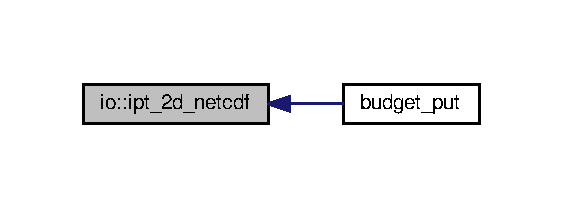
\includegraphics[width=270pt]{namespaceio_aff87bbb9c43d6db1fedd086586aab0c6_icgraph}
\end{center}
\end{figure}


\index{io@{io}!ipt\+\_\+2draw\+\_\+netcdf@{ipt\+\_\+2draw\+\_\+netcdf}}
\index{ipt\+\_\+2draw\+\_\+netcdf@{ipt\+\_\+2draw\+\_\+netcdf}!io@{io}}
\subsubsection[{\texorpdfstring{ipt\+\_\+2draw\+\_\+netcdf(\+I\+N\+P\+U\+T\+F\+I\+L\+E, V\+A\+R\+\_\+\+N\+A\+M\+E, V\+A\+R)}{ipt_2draw_netcdf(INPUTFILE, VAR_NAME, VAR)}}]{\setlength{\rightskip}{0pt plus 5cm}subroutine io\+::ipt\+\_\+2draw\+\_\+netcdf (
\begin{DoxyParamCaption}
\item[{character (len=$\ast$), intent(in)}]{I\+N\+P\+U\+T\+F\+I\+LE, }
\item[{character (len=$\ast$), intent(in)}]{V\+A\+R\+\_\+\+N\+A\+ME, }
\item[{real (kind=rk8), dimension(\+:), intent(out), allocatable}]{V\+AR}
\end{DoxyParamCaption}
)}\hypertarget{namespaceio_ac91ebbbf1426451d33f3e32b08f70aee}{}\label{namespaceio_ac91ebbbf1426451d33f3e32b08f70aee}


Definition at line 1614 of file io.\+f90.


\begin{DoxyCode}
1614     \textcolor{keywordtype}{USE }\hyperlink{namespaceportable}{portable}
1615     \textcolor{keywordtype}{USE }netcdf
1616 
1617     \textcolor{keywordtype}{IMPLICIT NONE}
1618 
1619     \textcolor{keywordtype}{CHARACTER (LEN=*)}, \textcolor{keywordtype}{INTENT(IN)}                                       :: inputfile    \textcolor{comment}{! Name of the input
       file.}
1620     \textcolor{keywordtype}{CHARACTER (LEN=*)}, \textcolor{keywordtype}{INTENT(IN)}                                       :: var\_name     \textcolor{comment}{! Name of the
       variable to read.}
1621     \textcolor{keywordtype}{REAL (KIND=RK8)}, \textcolor{keywordtype}{DIMENSION(:)}, \textcolor{keywordtype}{INTENT(OUT)}, \textcolor{keywordtype}{ALLOCATABLE}             :: var          \textcolor{comment}{! Holds the data we
       are reading.}
1622 
1623 
1624     \textcolor{comment}{!}
1625     \textcolor{comment}{! Local variables.}
1626     \textcolor{comment}{!}
1627     \textcolor{keywordtype}{INTEGER (KIND=IK4)}          :: ncid                                                 \textcolor{comment}{! ID of NetCDF
       file.}
1628     \textcolor{keywordtype}{INTEGER (KIND=IK4)}          :: t\_dim\_id                                             \textcolor{comment}{! Time dimension
       ID.}
1629     \textcolor{keywordtype}{INTEGER (KIND=IK4)}          :: t\_dim\_len                                            \textcolor{comment}{! Length of the
       time dimension.}
1630     \textcolor{keywordtype}{INTEGER (KIND=IK4)}          :: var\_id                                               \textcolor{comment}{! Variable ID.}
1631     \textcolor{keywordtype}{INTEGER (KIND=IK4)}          :: memst                                                \textcolor{comment}{! Status of memory
       allocations.}
1632     \textcolor{keywordtype}{INTEGER (KIND=IK4)}          :: iost                                                 \textcolor{comment}{! I/O status.}
1633 
1634     \textcolor{comment}{!}
1635     \textcolor{comment}{! Open the NetCDF file.}
1636     \textcolor{comment}{!}
1637     iost    = nf90\_open(inputfile, nf90\_nowrite, ncid)
1638     \textcolor{keywordflow}{IF} (iost .NE. nf90\_noerr) \textcolor{keywordflow}{THEN}
1639         print *,\textcolor{stringliteral}{'E: '},nf90\_strerror(iost)
1640         \textcolor{keywordflow}{GO TO} 9999
1641 \textcolor{keywordflow}{    END IF}
1642 
1643     \textcolor{comment}{!}
1644     \textcolor{comment}{! Get the time dimension ID, and the length of the dimension.}
1645     \textcolor{comment}{!}
1646     iost    = nf90\_inq\_dimid(ncid, \textcolor{stringliteral}{"time"}, t\_dim\_id)                            \textcolor{comment}{! Time steps.}
1647     \textcolor{keywordflow}{IF} (iost .NE. nf90\_noerr) \textcolor{keywordflow}{THEN}
1648         print *,\textcolor{stringliteral}{'E: '},nf90\_strerror(iost)
1649         \textcolor{keywordflow}{GO TO} 9999
1650 \textcolor{keywordflow}{    END IF}
1651     iost    = nf90\_inquire\_dimension(ncid, t\_dim\_id, len=t\_dim\_len)             \textcolor{comment}{! Get the time dimension
       length.}
1652     \textcolor{keywordflow}{IF} (iost .NE. nf90\_noerr) \textcolor{keywordflow}{THEN}
1653         print *,\textcolor{stringliteral}{'E: '},nf90\_strerror(iost)
1654         \textcolor{keywordflow}{GO TO} 9999
1655 \textcolor{keywordflow}{    END IF}
1656 
1657     \textcolor{comment}{!}
1658     \textcolor{comment}{! Allocate enough memory to hold all the data. Be paranoid ... check that arrays have not already been
       allocated.}
1659     \textcolor{comment}{!}
1660     \textcolor{keywordflow}{IF} (\textcolor{keyword}{ALLOCATED}(var))           \textcolor{keyword}{DEALLOCATE}(var)
1661     \textcolor{keyword}{ALLOCATE}(var(t\_dim\_len), stat=memst)
1662     \textcolor{keywordflow}{IF} (memst .NE. 0) \textcolor{keywordflow}{THEN}
1663         print *,\textcolor{stringliteral}{'E: Unable to allocate memory to hold data'}
1664         \textcolor{keywordflow}{GO TO} 9999
1665 \textcolor{keywordflow}{    END IF}
1666 
1667     \textcolor{comment}{!}
1668     \textcolor{comment}{! Get the variable IDs.}
1669     \textcolor{comment}{!}
1670     iost = nf90\_inq\_varid(ncid, var\_name, var\_id)
1671     \textcolor{keywordflow}{IF} (iost .NE. nf90\_noerr) \textcolor{keywordflow}{THEN}
1672         print *,\textcolor{stringliteral}{'E: '},nf90\_strerror(iost)
1673         \textcolor{keywordflow}{GO TO} 9999
1674 \textcolor{keywordflow}{    END IF}
1675 
1676     \textcolor{comment}{!}
1677     \textcolor{comment}{! Read the data.}
1678     \textcolor{comment}{!}
1679     iost = nf90\_get\_var(ncid, var\_id, var)
1680     \textcolor{keywordflow}{IF} (iost .NE. nf90\_noerr) \textcolor{keywordflow}{THEN}
1681         print *,\textcolor{stringliteral}{'E: '},nf90\_strerror(iost)
1682         \textcolor{keywordflow}{GO TO} 9999
1683 \textcolor{keywordflow}{    END IF}
1684 
1685     \textcolor{comment}{!}
1686     \textcolor{comment}{! Close the NetCDF file.}
1687     \textcolor{comment}{!}
1688     iost    = nf90\_close(ncid)
1689     \textcolor{keywordflow}{IF} (iost .NE. nf90\_noerr) \textcolor{keywordflow}{THEN}
1690         print *,\textcolor{stringliteral}{'E: '},nf90\_strerror(iost)
1691         \textcolor{keywordflow}{GO TO} 9999
1692 \textcolor{keywordflow}{    END IF}
1693 
1694     9999 \textcolor{keywordflow}{CONTINUE}       \textcolor{comment}{! Errors will be sent here.}
1695 
\end{DoxyCode}


Here is the caller graph for this function\+:\nopagebreak
\begin{figure}[H]
\begin{center}
\leavevmode
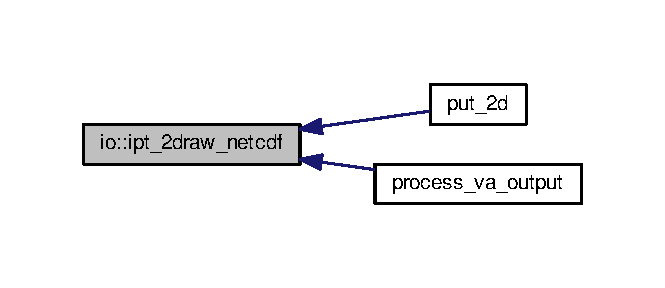
\includegraphics[width=319pt]{namespaceio_ac91ebbbf1426451d33f3e32b08f70aee_icgraph}
\end{center}
\end{figure}


\index{io@{io}!ipt\+\_\+3d\+\_\+netcdf@{ipt\+\_\+3d\+\_\+netcdf}}
\index{ipt\+\_\+3d\+\_\+netcdf@{ipt\+\_\+3d\+\_\+netcdf}!io@{io}}
\subsubsection[{\texorpdfstring{ipt\+\_\+3d\+\_\+netcdf(\+I\+N\+P\+U\+T\+F\+I\+L\+E, D\+U, V\+U, D\+S, T, S\+T\+N, W\+E\+I\+G\+H\+T, L\+E\+V, B\+O\+U\+N\+D\+A\+R\+Y, S\+T\+R\+U, S\+T\+R\+S)}{ipt_3d_netcdf(INPUTFILE, DU, VU, DS, T, STN, WEIGHT, LEV, BOUNDARY, STRU, STRS)}}]{\setlength{\rightskip}{0pt plus 5cm}subroutine io\+::ipt\+\_\+3d\+\_\+netcdf (
\begin{DoxyParamCaption}
\item[{character (len=$\ast$), intent(in)}]{I\+N\+P\+U\+T\+F\+I\+LE, }
\item[{real (kind=rk8), dimension(\+:,\+:,\+:,\+:), intent(out), optional, allocatable}]{DU, }
\item[{character (len=64), dimension(\+:), intent(out), optional, allocatable}]{VU, }
\item[{real (kind=rk8), dimension(\+:,\+:,\+:), intent(out), optional, allocatable}]{DS, }
\item[{real (kind=rk8), dimension(\+:), intent(out), optional, allocatable}]{T, }
\item[{character (len=64), dimension(\+:), intent(out), optional, allocatable}]{S\+TN, }
\item[{real (kind=rk8), dimension(\+:), intent(out), optional, allocatable}]{W\+E\+I\+G\+HT, }
\item[{real (kind=rk8), dimension(\+:), intent(out), optional, allocatable}]{L\+EV, }
\item[{integer (kind=ik4), dimension(\+:,\+:), intent(out), optional, allocatable}]{B\+O\+U\+N\+D\+A\+RY, }
\item[{integer (kind=ik4), dimension(\+:), intent(out), optional, allocatable}]{S\+T\+RU, }
\item[{integer (kind=ik4), dimension(\+:), intent(out), optional, allocatable}]{S\+T\+RS}
\end{DoxyParamCaption}
)}\hypertarget{namespaceio_a0f9f8edb9a7173638e450ce3c4db7844}{}\label{namespaceio_a0f9f8edb9a7173638e450ce3c4db7844}


Definition at line 618 of file io.\+f90.


\begin{DoxyCode}
618     \textcolor{keywordtype}{USE }\hyperlink{namespaceportable}{portable}
619     \textcolor{keywordtype}{USE }netcdf
620 
621     \textcolor{keywordtype}{IMPLICIT NONE}
622 
623     \textcolor{keywordtype}{CHARACTER (LEN=*)}, \textcolor{keywordtype}{INTENT(IN)}                                           :: inputfile    \textcolor{comment}{! Name of the
       input file.}
624     \textcolor{keywordtype}{REAL (KIND=RK8)}, \textcolor{keywordtype}{DIMENSION(:,:,:,:)}, \textcolor{keywordtype}{INTENT(OUT)}, \textcolor{keywordtype}{ALLOCATABLE}, \textcolor{keywordtype}{OPTIONAL} :: du           \textcolor{comment}{! The 3D data.}
625     \textcolor{keywordtype}{CHARACTER (LEN=64)}, \textcolor{keywordtype}{DIMENSION(:)}, \textcolor{keywordtype}{INTENT(OUT)}, \textcolor{keywordtype}{ALLOCATABLE}, \textcolor{keywordtype}{OPTIONAL}    :: vu           \textcolor{comment}{! Names of the
       variables in DU.}
626     \textcolor{keywordtype}{REAL (KIND=RK8)}, \textcolor{keywordtype}{DIMENSION(:,:,:)}, \textcolor{keywordtype}{INTENT(OUT)}, \textcolor{keywordtype}{ALLOCATABLE}, \textcolor{keywordtype}{OPTIONAL}   :: ds           \textcolor{comment}{! Surface level
       data.}
627     \textcolor{keywordtype}{REAL (KIND=RK8)}, \textcolor{keywordtype}{DIMENSION(:)}, \textcolor{keywordtype}{INTENT(OUT)}, \textcolor{keywordtype}{ALLOCATABLE}, \textcolor{keywordtype}{OPTIONAL}       :: t            \textcolor{comment}{! Time steps.  
              }
628     \textcolor{keywordtype}{CHARACTER (LEN=64)}, \textcolor{keywordtype}{DIMENSION(:)}, \textcolor{keywordtype}{INTENT(OUT)}, \textcolor{keywordtype}{ALLOCATABLE}, \textcolor{keywordtype}{OPTIONAL}    :: stn          \textcolor{comment}{! Names of the
       stations.}
629     \textcolor{keywordtype}{REAL (KIND=RK8)}, \textcolor{keywordtype}{DIMENSION(:)}, \textcolor{keywordtype}{INTENT(OUT)}, \textcolor{keywordtype}{ALLOCATABLE}, \textcolor{keywordtype}{OPTIONAL}       :: lev          \textcolor{comment}{! Vertical
       levels in analysis.}
630     \textcolor{keywordtype}{INTEGER (KIND=IK4)}, \textcolor{keywordtype}{DIMENSION(:,:)}, \textcolor{keywordtype}{INTENT(OUT)}, \textcolor{keywordtype}{ALLOCATABLE}, \textcolor{keywordtype}{OPTIONAL}  :: boundary     \textcolor{comment}{! Boundary
       array.}
631     \textcolor{keywordtype}{INTEGER (KIND=IK4)}, \textcolor{keywordtype}{DIMENSION(:)}, \textcolor{keywordtype}{INTENT(OUT)}, \textcolor{keywordtype}{ALLOCATABLE}, \textcolor{keywordtype}{OPTIONAL}    :: stru         \textcolor{comment}{! STRU array.}
632     \textcolor{keywordtype}{INTEGER (KIND=IK4)}, \textcolor{keywordtype}{DIMENSION(:)}, \textcolor{keywordtype}{INTENT(OUT)}, \textcolor{keywordtype}{ALLOCATABLE}, \textcolor{keywordtype}{OPTIONAL}    :: strs         \textcolor{comment}{! STRS array.}
633     \textcolor{keywordtype}{REAL (KIND=RK8)}, \textcolor{keywordtype}{DIMENSION(:)}, \textcolor{keywordtype}{INTENT(OUT)}, \textcolor{keywordtype}{ALLOCATABLE}, \textcolor{keywordtype}{OPTIONAL}       :: weight       \textcolor{comment}{! WEIGHT array.}
634 
635     \textcolor{comment}{!}
636     \textcolor{comment}{! Local variables.}
637     \textcolor{comment}{!}
638     \textcolor{keywordtype}{INTEGER (KIND=IK4)}          :: ncid                                                 \textcolor{comment}{! ID of NetCDF
       file.}
639 
640     \textcolor{keywordtype}{INTEGER (KIND=IK4)}          :: t\_dim\_id                                             \textcolor{comment}{! Time dimension
       ID.}
641     \textcolor{keywordtype}{INTEGER (KIND=IK4)}          :: t\_dim\_len                                            \textcolor{comment}{! Number of time
       steps.}
642     \textcolor{keywordtype}{INTEGER (KIND=IK4)}          :: stn\_dim\_id                                           \textcolor{comment}{! Station dimension
       ID.}
643     \textcolor{keywordtype}{INTEGER (KIND=IK4)}          :: stn\_dim\_len                                          \textcolor{comment}{! Number of
       stations.}
644     \textcolor{keywordtype}{INTEGER (KIND=IK4)}          :: lev\_dim\_id                                           \textcolor{comment}{! Vertical level
       dimension ID.}
645     \textcolor{keywordtype}{INTEGER (KIND=IK4)}          :: lev\_dim\_len                                          \textcolor{comment}{! Number of
       vertical levels.}
646     \textcolor{keywordtype}{INTEGER (KIND=IK4)}          :: var\_dim\_id                                           \textcolor{comment}{! Variable
       dimension ID.}
647     \textcolor{keywordtype}{INTEGER (KIND=IK4)}          :: var\_dim\_len                                          \textcolor{comment}{! Number of
       variables.}
648     \textcolor{keywordtype}{INTEGER (KIND=IK4)}          :: str\_dim\_id                                           \textcolor{comment}{! String dimension
       ID.}
649     \textcolor{keywordtype}{INTEGER (KIND=IK4)}          :: str\_dim\_len                                          \textcolor{comment}{! String length.}
650     \textcolor{keywordtype}{INTEGER (KIND=IK4)}          :: bnd\_dim\_id                                           \textcolor{comment}{! Dimension used
       for BOUNDARY array.}
651     \textcolor{keywordtype}{INTEGER (KIND=IK4)}          :: bnd\_dim\_len                                          \textcolor{comment}{! Length of BND
       dimension.}
652     \textcolor{keywordtype}{INTEGER (KIND=IK4)}          :: stru\_dim\_id                                          \textcolor{comment}{! Dimension used
       for STRU array.}
653     \textcolor{keywordtype}{INTEGER (KIND=IK4)}          :: stru\_dim\_len                                         \textcolor{comment}{! Length of STRU
       dimension.}
654     \textcolor{keywordtype}{INTEGER (KIND=IK4)}          :: strs\_dim\_id                                          \textcolor{comment}{! Dimension used
       for STRS array.}
655     \textcolor{keywordtype}{INTEGER (KIND=IK4)}          :: strs\_dim\_len                                         \textcolor{comment}{! Length of STRS
       dimension.}
656     \textcolor{keywordtype}{INTEGER (KIND=IK4)}          :: weight\_dim\_id                                        \textcolor{comment}{! Dimension used
       for WEIGHT array.}
657     \textcolor{keywordtype}{INTEGER (KIND=IK4)}          :: weight\_dim\_len                                       \textcolor{comment}{! Length of WEIGHT
       dimension.}
658 
659     \textcolor{keywordtype}{INTEGER (KIND=IK4)}          :: t\_var\_id                                             \textcolor{comment}{! Time variable ID.}
660     \textcolor{keywordtype}{INTEGER (KIND=IK4)}          :: du\_var\_id                                            \textcolor{comment}{! 3D data variable
       ID.}
661     \textcolor{keywordtype}{INTEGER (KIND=IK4)}          :: ds\_var\_id                                            \textcolor{comment}{! Surface data
       variable ID.}
662     \textcolor{keywordtype}{INTEGER (KIND=IK4)}          :: stn\_var\_id                                           \textcolor{comment}{! Station names
       variable ID.}
663     \textcolor{keywordtype}{INTEGER (KIND=IK4)}          :: lev\_var\_id                                           \textcolor{comment}{! Vertical levels
       variable ID.}
664     \textcolor{keywordtype}{INTEGER (KIND=IK4)}          :: vu\_var\_id                                            \textcolor{comment}{! Variable names
       variable ID.}
665     \textcolor{keywordtype}{INTEGER (KIND=IK4)}          :: boundary\_var\_id                                      \textcolor{comment}{! ID of BOUNDARY
       variable.}
666     \textcolor{keywordtype}{INTEGER (KIND=IK4)}          :: stru\_var\_id                                          \textcolor{comment}{! ID of STRU
       variable.}
667     \textcolor{keywordtype}{INTEGER (KIND=IK4)}          :: strs\_var\_id                                          \textcolor{comment}{! ID of STRS
       variable.}
668     \textcolor{keywordtype}{INTEGER (KIND=IK4)}          :: weight\_var\_id                                        \textcolor{comment}{! ID of WEIGHT
       variable.}
669 
670     \textcolor{keywordtype}{INTEGER (KIND=IK4)}          :: memst                                                \textcolor{comment}{! Status of memory
       allocations.}
671     \textcolor{keywordtype}{INTEGER (KIND=IK4)}          :: iost                                                 \textcolor{comment}{! I/O status.}
672     \textcolor{keywordtype}{LOGICAL}                     :: ncerror
673 
674     iost    = nf90\_noerr
675     ncerror = .false.
676     \textcolor{comment}{!}
677     \textcolor{comment}{! Open the NetCDF file.}
678     \textcolor{comment}{!}
679     iost    = nf90\_open(inputfile, nf90\_nowrite, ncid)
680     \textcolor{keywordflow}{IF} (iost .NE. nf90\_noerr) \textcolor{keywordflow}{GO TO} 9999
681 
682     \textcolor{comment}{!}
683     \textcolor{comment}{! Get the dimension IDs, and the length of the dimensions.}
684     \textcolor{comment}{!}
685     iost    = nf90\_inq\_dimid(ncid, \textcolor{stringliteral}{"time"}, t\_dim\_id)                            \textcolor{comment}{! Time steps.}
686     \textcolor{keywordflow}{IF} (iost .NE. nf90\_noerr) \textcolor{keywordflow}{GO TO} 9999
687     iost    = nf90\_inquire\_dimension(ncid, t\_dim\_id, len=t\_dim\_len)             \textcolor{comment}{! Get the number of time
       steps.}
688     \textcolor{keywordflow}{IF} (iost .NE. nf90\_noerr) \textcolor{keywordflow}{GO TO} 9999
689 
690     iost    = nf90\_inq\_dimid(ncid, \textcolor{stringliteral}{"stations"}, stn\_dim\_id)                      \textcolor{comment}{! Time steps.}
691     \textcolor{keywordflow}{IF} (iost .NE. nf90\_noerr) \textcolor{keywordflow}{GO TO} 9999
692     iost    = nf90\_inquire\_dimension(ncid, stn\_dim\_id, len=stn\_dim\_len)         \textcolor{comment}{! Get the number of
       stations.}
693     \textcolor{keywordflow}{IF} (iost .NE. nf90\_noerr) \textcolor{keywordflow}{GO TO} 9999
694 
695     iost    = nf90\_inq\_dimid(ncid, \textcolor{stringliteral}{"levels"}, lev\_dim\_id)                        \textcolor{comment}{! Vertical levels.}
696     \textcolor{keywordflow}{IF} (iost .NE. nf90\_noerr) \textcolor{keywordflow}{GO TO} 9999
697     iost    = nf90\_inquire\_dimension(ncid, lev\_dim\_id, len=lev\_dim\_len)         \textcolor{comment}{! Number of vertical
       levels.}
698     \textcolor{keywordflow}{IF} (iost .NE. nf90\_noerr) \textcolor{keywordflow}{GO TO} 9999
699 
700     iost    = nf90\_inq\_dimid(ncid, \textcolor{stringliteral}{"variables"}, var\_dim\_id)                     \textcolor{comment}{! Variables.}
701     \textcolor{keywordflow}{IF} (iost .NE. nf90\_noerr) \textcolor{keywordflow}{GO TO} 9999
702     iost    = nf90\_inquire\_dimension(ncid, var\_dim\_id, len=var\_dim\_len)         \textcolor{comment}{! Get the number of
       variables.}
703     \textcolor{keywordflow}{IF} (iost .NE. nf90\_noerr) \textcolor{keywordflow}{GO TO} 9999
704 
705     iost    = nf90\_inq\_dimid(ncid, \textcolor{stringliteral}{"string"}, str\_dim\_id)                        \textcolor{comment}{! String dimension.}
706     \textcolor{keywordflow}{IF} (iost .NE. nf90\_noerr) \textcolor{keywordflow}{GO TO} 9999
707     iost    = nf90\_inquire\_dimension(ncid, str\_dim\_id, len=str\_dim\_len)         \textcolor{comment}{! String length.}
708     \textcolor{keywordflow}{IF} (iost .NE. nf90\_noerr) \textcolor{keywordflow}{GO TO} 9999
709 
710     iost    = nf90\_inq\_dimid(ncid, \textcolor{stringliteral}{"bnd"}, bnd\_dim\_id)                           \textcolor{comment}{! bnd dimension.}
711     \textcolor{keywordflow}{IF} (iost .NE. nf90\_noerr) \textcolor{keywordflow}{GO TO} 9999
712     iost    = nf90\_inquire\_dimension(ncid, bnd\_dim\_id, len=bnd\_dim\_len)         \textcolor{comment}{! bnd dimension length
       (should be 3).}
713     \textcolor{keywordflow}{IF} (iost .NE. nf90\_noerr) \textcolor{keywordflow}{GO TO} 9999
714 
715     iost    = nf90\_inq\_dimid(ncid, \textcolor{stringliteral}{"stru"}, stru\_dim\_id)                         \textcolor{comment}{! stru dimension.}
716     \textcolor{keywordflow}{IF} (iost .NE. nf90\_noerr) \textcolor{keywordflow}{GO TO} 9999
717     iost    = nf90\_inquire\_dimension(ncid, stru\_dim\_id, len=stru\_dim\_len)       \textcolor{comment}{! stru dimension length.}
718     \textcolor{keywordflow}{IF} (iost .NE. nf90\_noerr) \textcolor{keywordflow}{GO TO} 9999
719 
720     iost    = nf90\_inq\_dimid(ncid, \textcolor{stringliteral}{"strs"}, strs\_dim\_id)                         \textcolor{comment}{! strs dimension.}
721     \textcolor{keywordflow}{IF} (iost .NE. nf90\_noerr) \textcolor{keywordflow}{GO TO} 9999
722     iost    = nf90\_inquire\_dimension(ncid, strs\_dim\_id, len=strs\_dim\_len)       \textcolor{comment}{! strs dimension length.}
723     \textcolor{keywordflow}{IF} (iost .NE. nf90\_noerr) \textcolor{keywordflow}{GO TO} 9999
724 
725     iost    = nf90\_inq\_dimid(ncid, \textcolor{stringliteral}{"weight"}, weight\_dim\_id)                     \textcolor{comment}{! weight dimension.}
726     \textcolor{keywordflow}{IF} (iost .NE. nf90\_noerr) \textcolor{keywordflow}{GO TO} 9999
727     iost    = nf90\_inquire\_dimension(ncid, weight\_dim\_id, len=weight\_dim\_len)   \textcolor{comment}{! weight dimension length.}
728     \textcolor{keywordflow}{IF} (iost .NE. nf90\_noerr) \textcolor{keywordflow}{GO TO} 9999
729 
730     \textcolor{comment}{!}
731     \textcolor{comment}{! Read in the data. Only read those variables which the user requests in the optional subroutine
       arguments.}
732     \textcolor{comment}{! When allocating memory, be paranoid, check it hasn't already been allocated.}
733     \textcolor{comment}{!}
734     \textcolor{keywordflow}{IF} (\textcolor{keyword}{PRESENT}(du)) \textcolor{keywordflow}{THEN}
735         \textcolor{keywordflow}{IF} (\textcolor{keyword}{ALLOCATED}(du))          \textcolor{keyword}{DEALLOCATE}(du)
736         \textcolor{keyword}{ALLOCATE}(du(var\_dim\_len,lev\_dim\_len,stn\_dim\_len,t\_dim\_len), stat=memst)
737         \textcolor{keywordflow}{IF} (memst .NE. 0) \textcolor{keywordflow}{THEN}
738             print *,\textcolor{stringliteral}{'E: IPT\_3D\_NETCDF: Unable to allocate memory to hold DU'}
739             stop \textcolor{stringliteral}{'1'}
740 \textcolor{keywordflow}{        END IF}
741         iost = nf90\_inq\_varid(ncid, \textcolor{stringliteral}{"du"}, du\_var\_id)
742         \textcolor{keywordflow}{IF} (iost .NE. nf90\_noerr) \textcolor{keywordflow}{GO TO} 9999
743         iost = nf90\_get\_var(ncid, du\_var\_id, du)
744         \textcolor{keywordflow}{IF} (iost .NE. nf90\_noerr) \textcolor{keywordflow}{GO TO} 9999
745 \textcolor{keywordflow}{    END IF}
746     \textcolor{keywordflow}{IF} (\textcolor{keyword}{PRESENT}(vu)) \textcolor{keywordflow}{THEN}
747         \textcolor{keywordflow}{IF} (\textcolor{keyword}{ALLOCATED}(vu))          \textcolor{keyword}{DEALLOCATE}(vu)
748         \textcolor{keyword}{ALLOCATE}(vu(var\_dim\_len), stat=memst)
749         \textcolor{keywordflow}{IF} (memst .NE. 0) \textcolor{keywordflow}{THEN}
750             print *,\textcolor{stringliteral}{'E: IPT\_3D\_NETCDF: Unable to allocate memory to hold VU'}
751             stop \textcolor{stringliteral}{'1'}
752 \textcolor{keywordflow}{        END IF}
753         iost = nf90\_inq\_varid(ncid, \textcolor{stringliteral}{"variables"}, vu\_var\_id)
754         \textcolor{keywordflow}{IF} (iost .NE. nf90\_noerr) \textcolor{keywordflow}{GO TO} 9999
755         iost = nf90\_get\_var(ncid, vu\_var\_id, vu)
756         \textcolor{keywordflow}{IF} (iost .NE. nf90\_noerr) \textcolor{keywordflow}{GO TO} 9999
757 \textcolor{keywordflow}{    END IF}
758 
759     \textcolor{keywordflow}{IF} (\textcolor{keyword}{PRESENT}(ds)) \textcolor{keywordflow}{THEN}
760         \textcolor{keywordflow}{IF} (\textcolor{keyword}{ALLOCATED}(ds))          \textcolor{keyword}{DEALLOCATE}(ds)
761         \textcolor{keyword}{ALLOCATE}(ds(var\_dim\_len,stn\_dim\_len,t\_dim\_len), stat=memst)
762         \textcolor{keywordflow}{IF} (memst .NE. 0) \textcolor{keywordflow}{THEN}
763             print *,\textcolor{stringliteral}{'E: IPT\_3D\_NETCDF: Unable to allocate memory to hold DS'}
764             stop \textcolor{stringliteral}{'1'}
765 \textcolor{keywordflow}{        END IF}
766         iost = nf90\_inq\_varid(ncid, \textcolor{stringliteral}{"ds"}, ds\_var\_id)
767         \textcolor{keywordflow}{IF} (iost .NE. nf90\_noerr) \textcolor{keywordflow}{GO TO} 9999
768         iost = nf90\_get\_var(ncid, ds\_var\_id, ds)
769         \textcolor{keywordflow}{IF} (iost .NE. nf90\_noerr) \textcolor{keywordflow}{GO TO} 9999
770 \textcolor{keywordflow}{    END IF}
771 
772     \textcolor{keywordflow}{IF} (\textcolor{keyword}{PRESENT}(t)) \textcolor{keywordflow}{THEN}
773         \textcolor{keywordflow}{IF} (\textcolor{keyword}{ALLOCATED}(t))           \textcolor{keyword}{DEALLOCATE}(t)
774         \textcolor{keyword}{ALLOCATE}(t(t\_dim\_len), stat=memst)
775         \textcolor{keywordflow}{IF} (memst .NE. 0) \textcolor{keywordflow}{THEN}
776             print *,\textcolor{stringliteral}{'E: IPT\_3D\_NETCDF: Unable to allocate memory to hold T'}
777             stop \textcolor{stringliteral}{'1'}
778 \textcolor{keywordflow}{        END IF}
779         iost = nf90\_inq\_varid(ncid, \textcolor{stringliteral}{"time"}, t\_var\_id)
780         \textcolor{keywordflow}{IF} (iost .NE. nf90\_noerr) \textcolor{keywordflow}{GO TO} 9999
781         iost = nf90\_get\_var(ncid, t\_var\_id, t)
782         \textcolor{keywordflow}{IF} (iost .NE. nf90\_noerr) \textcolor{keywordflow}{GO TO} 9999
783 \textcolor{keywordflow}{    END IF}
784 
785     \textcolor{keywordflow}{IF} (\textcolor{keyword}{PRESENT}(stn)) \textcolor{keywordflow}{THEN}
786         \textcolor{keywordflow}{IF} (\textcolor{keyword}{ALLOCATED}(stn))         \textcolor{keyword}{DEALLOCATE}(stn)
787         \textcolor{keyword}{ALLOCATE}(stn(stn\_dim\_len), stat=memst)
788         \textcolor{keywordflow}{IF} (memst .NE. 0) \textcolor{keywordflow}{THEN}
789             print *,\textcolor{stringliteral}{'E: IPT\_3D\_NETCDF: Unable to allocate memory to hold STN'}
790             stop \textcolor{stringliteral}{'1'}
791 \textcolor{keywordflow}{        END IF}
792         iost = nf90\_inq\_varid(ncid, \textcolor{stringliteral}{"stations"}, stn\_var\_id)
793         \textcolor{keywordflow}{IF} (iost .NE. nf90\_noerr) \textcolor{keywordflow}{GO TO} 9999
794         iost = nf90\_get\_var(ncid, stn\_var\_id, stn)
795         \textcolor{keywordflow}{IF} (iost .NE. nf90\_noerr) \textcolor{keywordflow}{GO TO} 9999
796 \textcolor{keywordflow}{    END IF}
797 
798     \textcolor{keywordflow}{IF} (\textcolor{keyword}{PRESENT}(lev)) \textcolor{keywordflow}{THEN}
799         \textcolor{keywordflow}{IF} (\textcolor{keyword}{ALLOCATED}(lev))         \textcolor{keyword}{DEALLOCATE}(lev)
800         \textcolor{keyword}{ALLOCATE}(lev(lev\_dim\_len), stat=memst)
801         \textcolor{keywordflow}{IF} (memst .NE. 0) \textcolor{keywordflow}{THEN}
802             print *,\textcolor{stringliteral}{'E: IPT\_3D\_NETCDF: Unable to allocate memory to hold LEV'}
803             stop \textcolor{stringliteral}{'1'}
804 \textcolor{keywordflow}{        END IF}
805         iost = nf90\_inq\_varid(ncid, \textcolor{stringliteral}{"levels"}, lev\_var\_id)
806         \textcolor{keywordflow}{IF} (iost .NE. nf90\_noerr) \textcolor{keywordflow}{GO TO} 9999
807         iost = nf90\_get\_var(ncid, lev\_var\_id, lev)
808         \textcolor{keywordflow}{IF} (iost .NE. nf90\_noerr) \textcolor{keywordflow}{GO TO} 9999
809 \textcolor{keywordflow}{    END IF}
810 
811     \textcolor{keywordflow}{IF} (\textcolor{keyword}{PRESENT}(boundary)) \textcolor{keywordflow}{THEN}
812         \textcolor{keywordflow}{IF} (\textcolor{keyword}{ALLOCATED}(boundary))    \textcolor{keyword}{DEALLOCATE}(boundary)
813         \textcolor{keyword}{ALLOCATE}(boundary(bnd\_dim\_len,t\_dim\_len), stat=memst)
814         \textcolor{keywordflow}{IF} (memst .NE. 0) \textcolor{keywordflow}{THEN}
815             print *,\textcolor{stringliteral}{'E: IPT\_3D\_NETCDF: Unable to allocate memory to hold BOUNDARY'}
816             stop \textcolor{stringliteral}{'1'}
817 \textcolor{keywordflow}{        END IF}
818         iost = nf90\_inq\_varid(ncid, \textcolor{stringliteral}{"boundary"}, boundary\_var\_id)
819         \textcolor{keywordflow}{IF} (iost .NE. nf90\_noerr) \textcolor{keywordflow}{GO TO} 9999
820         iost = nf90\_get\_var(ncid, boundary\_var\_id, boundary)
821         \textcolor{keywordflow}{IF} (iost .NE. nf90\_noerr) \textcolor{keywordflow}{GO TO} 9999
822 \textcolor{keywordflow}{    END IF}
823 
824     \textcolor{keywordflow}{IF} (\textcolor{keyword}{PRESENT}(stru)) \textcolor{keywordflow}{THEN}
825         \textcolor{keywordflow}{IF} (\textcolor{keyword}{ALLOCATED}(stru))        \textcolor{keyword}{DEALLOCATE}(stru)
826         \textcolor{keyword}{ALLOCATE}(stru(stru\_dim\_len), stat=memst)
827         \textcolor{keywordflow}{IF} (memst .NE. 0) \textcolor{keywordflow}{THEN}
828             print *,\textcolor{stringliteral}{'E: IPT\_3D\_NETCDF: Unable to allocate memory to hold STRU'}
829             stop \textcolor{stringliteral}{'1'}
830 \textcolor{keywordflow}{        END IF}
831         iost = nf90\_inq\_varid(ncid, \textcolor{stringliteral}{"stru"}, stru\_var\_id)
832         \textcolor{keywordflow}{IF} (iost .NE. nf90\_noerr) \textcolor{keywordflow}{GO TO} 9999
833         iost = nf90\_get\_var(ncid, stru\_var\_id, stru)
834         \textcolor{keywordflow}{IF} (iost .NE. nf90\_noerr) \textcolor{keywordflow}{GO TO} 9999
835 \textcolor{keywordflow}{    END IF}
836 
837     \textcolor{keywordflow}{IF} (\textcolor{keyword}{PRESENT}(strs)) \textcolor{keywordflow}{THEN}
838         \textcolor{keywordflow}{IF} (\textcolor{keyword}{ALLOCATED}(strs))        \textcolor{keyword}{DEALLOCATE}(strs)
839         \textcolor{keyword}{ALLOCATE}(strs(strs\_dim\_len), stat=memst)
840         \textcolor{keywordflow}{IF} (memst .NE. 0) \textcolor{keywordflow}{THEN}
841             print *,\textcolor{stringliteral}{'E: IPT\_3D\_NETCDF: Unable to allocate memory to hold STRS'}
842             stop \textcolor{stringliteral}{'1'}
843 \textcolor{keywordflow}{        END IF}
844         iost = nf90\_inq\_varid(ncid, \textcolor{stringliteral}{"strs"}, strs\_var\_id)
845         \textcolor{keywordflow}{IF} (iost .NE. nf90\_noerr) \textcolor{keywordflow}{GO TO} 9999
846         iost = nf90\_get\_var(ncid, strs\_var\_id, strs)
847         \textcolor{keywordflow}{IF} (iost .NE. nf90\_noerr) \textcolor{keywordflow}{GO TO} 9999
848 \textcolor{keywordflow}{    END IF}
849 
850     \textcolor{keywordflow}{IF} (\textcolor{keyword}{PRESENT}(weight)) \textcolor{keywordflow}{THEN}
851         \textcolor{keywordflow}{IF} (\textcolor{keyword}{ALLOCATED}(weight))        \textcolor{keyword}{DEALLOCATE}(weight)
852         \textcolor{keyword}{ALLOCATE}(weight(weight\_dim\_len), stat=memst)
853         \textcolor{keywordflow}{IF} (memst .NE. 0) \textcolor{keywordflow}{THEN}
854             print *,\textcolor{stringliteral}{'E: IPT\_3D\_NETCDF: Unable to allocate memory to hold WEIGHT'}
855             stop \textcolor{stringliteral}{'1'}
856 \textcolor{keywordflow}{        END IF}
857         iost = nf90\_inq\_varid(ncid, \textcolor{stringliteral}{"weight"}, weight\_var\_id)
858         \textcolor{keywordflow}{IF} (iost .NE. nf90\_noerr) \textcolor{keywordflow}{GO TO} 9999
859         iost = nf90\_get\_var(ncid, weight\_var\_id, weight)
860         \textcolor{keywordflow}{IF} (iost .NE. nf90\_noerr) \textcolor{keywordflow}{GO TO} 9999
861 \textcolor{keywordflow}{    END IF}
862 
863     \textcolor{comment}{!}
864     \textcolor{comment}{! Close the NetCDF file.}
865     \textcolor{comment}{!}
866     iost    = nf90\_close(ncid)
867     \textcolor{keywordflow}{IF} (iost .NE. nf90\_noerr) \textcolor{keywordflow}{GO TO} 9999
868 
869     \textcolor{comment}{!}
870     \textcolor{comment}{! Catch any NetCDF errors here.}
871     \textcolor{comment}{!}
872     9999 \textcolor{keywordflow}{CONTINUE}
873     \textcolor{keywordflow}{IF} (ncerror) \textcolor{keywordflow}{THEN}
874         print *,\textcolor{stringliteral}{'E: IPT\_3D\_NETCDF: NetCDF error encountered'}
875         \textcolor{keywordflow}{IF} (iost .NE. nf90\_noerr) \textcolor{keywordflow}{THEN}
876             print *, trim(nf90\_strerror(iost))
877 \textcolor{keywordflow}{        END IF}
878         stop \textcolor{stringliteral}{'1'}
879 \textcolor{keywordflow}{    END IF}
880 
\end{DoxyCode}


Here is the caller graph for this function\+:\nopagebreak
\begin{figure}[H]
\begin{center}
\leavevmode
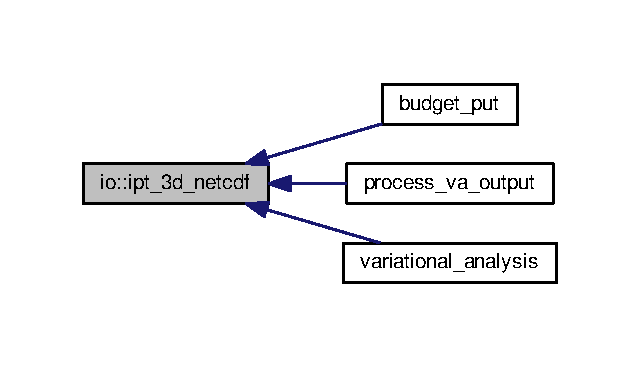
\includegraphics[width=307pt]{namespaceio_a0f9f8edb9a7173638e450ce3c4db7844_icgraph}
\end{center}
\end{figure}


\index{io@{io}!ipt\+\_\+budget\+\_\+netcdf@{ipt\+\_\+budget\+\_\+netcdf}}
\index{ipt\+\_\+budget\+\_\+netcdf@{ipt\+\_\+budget\+\_\+netcdf}!io@{io}}
\subsubsection[{\texorpdfstring{ipt\+\_\+budget\+\_\+netcdf(\+I\+N\+P\+U\+T\+F\+I\+L\+E, B\+U\+D\+G\+E\+T\+\_\+\+C\+O\+L\+U\+M\+N, B\+U\+D\+G\+E\+T\+\_\+\+L\+A\+Y\+E\+R, V\+B\+U\+D\+G\+E\+T\+\_\+\+C\+O\+L\+U\+M\+N, V\+B\+U\+D\+G\+E\+T\+\_\+\+L\+A\+Y\+E\+R, A\+V\+E\+\_\+\+Q\+S, A\+V\+E\+\_\+\+S\+S, P, T)}{ipt_budget_netcdf(INPUTFILE, BUDGET_COLUMN, BUDGET_LAYER, VBUDGET_COLUMN, VBUDGET_LAYER, AVE_QS, AVE_SS, P, T)}}]{\setlength{\rightskip}{0pt plus 5cm}subroutine io\+::ipt\+\_\+budget\+\_\+netcdf (
\begin{DoxyParamCaption}
\item[{character (len=$\ast$), intent(in)}]{I\+N\+P\+U\+T\+F\+I\+LE, }
\item[{real (kind=rk8), dimension(\+:,\+:,\+:), intent(out), optional, allocatable}]{B\+U\+D\+G\+E\+T\+\_\+\+C\+O\+L\+U\+MN, }
\item[{real (kind=rk8), dimension(\+:,\+:,\+:,\+:), intent(out), optional, allocatable}]{B\+U\+D\+G\+E\+T\+\_\+\+L\+A\+Y\+ER, }
\item[{character (len=64), dimension(\+:,\+:), intent(out), optional, allocatable}]{V\+B\+U\+D\+G\+E\+T\+\_\+\+C\+O\+L\+U\+MN, }
\item[{character (len=64), dimension(\+:,\+:), intent(out), optional, allocatable}]{V\+B\+U\+D\+G\+E\+T\+\_\+\+L\+A\+Y\+ER, }
\item[{real (kind=rk8), dimension(\+:), intent(out), optional, allocatable}]{A\+V\+E\+\_\+\+QS, }
\item[{real (kind=rk8), dimension(\+:), intent(out), optional, allocatable}]{A\+V\+E\+\_\+\+SS, }
\item[{real (kind=rk8), dimension(\+:), intent(out), optional, allocatable}]{P, }
\item[{real (kind=rk8), dimension(\+:), intent(out), optional, allocatable}]{T}
\end{DoxyParamCaption}
)}\hypertarget{namespaceio_aba707a842ac0a3e2e9def20af0b36c32}{}\label{namespaceio_aba707a842ac0a3e2e9def20af0b36c32}


Definition at line 1070 of file io.\+f90.


\begin{DoxyCode}
1070     \textcolor{keywordtype}{USE }\hyperlink{namespaceportable}{portable}
1071     \textcolor{keywordtype}{USE }netcdf
1072 
1073     \textcolor{keywordtype}{IMPLICIT NONE}
1074 
1075     \textcolor{keywordtype}{CHARACTER (LEN=*)}, \textcolor{keywordtype}{INTENT(IN)}                                           :: inputfile    \textcolor{comment}{! Name of the
       input file.}
1076     \textcolor{keywordtype}{REAL (KIND=RK8)}, \textcolor{keywordtype}{DIMENSION(:,:,:)}, \textcolor{keywordtype}{INTENT(OUT)}, \textcolor{keywordtype}{ALLOCATABLE}, \textcolor{keywordtype}{OPTIONAL}   :: budget\_column
1077     \textcolor{keywordtype}{REAL (KIND=RK8)}, \textcolor{keywordtype}{DIMENSION(:,:,:,:)}, \textcolor{keywordtype}{INTENT(OUT)}, \textcolor{keywordtype}{ALLOCATABLE}, \textcolor{keywordtype}{OPTIONAL} :: budget\_layer
1078     \textcolor{keywordtype}{CHARACTER (LEN=64)}, \textcolor{keywordtype}{DIMENSION(:,:)}, \textcolor{keywordtype}{INTENT(OUT)}, \textcolor{keywordtype}{ALLOCATABLE}, \textcolor{keywordtype}{OPTIONAL}  :: vbudget\_column
1079     \textcolor{keywordtype}{CHARACTER (LEN=64)}, \textcolor{keywordtype}{DIMENSION(:,:)}, \textcolor{keywordtype}{INTENT(OUT)}, \textcolor{keywordtype}{ALLOCATABLE}, \textcolor{keywordtype}{OPTIONAL}  :: vbudget\_layer
1080     \textcolor{keywordtype}{REAL (KIND=RK8)}, \textcolor{keywordtype}{DIMENSION(:)}, \textcolor{keywordtype}{INTENT(OUT)}, \textcolor{keywordtype}{ALLOCATABLE}, \textcolor{keywordtype}{OPTIONAL}       :: ave\_qs
1081     \textcolor{keywordtype}{REAL (KIND=RK8)}, \textcolor{keywordtype}{DIMENSION(:)}, \textcolor{keywordtype}{INTENT(OUT)}, \textcolor{keywordtype}{ALLOCATABLE}, \textcolor{keywordtype}{OPTIONAL}       :: ave\_ss
1082     \textcolor{keywordtype}{REAL (KIND=RK8)}, \textcolor{keywordtype}{DIMENSION(:)}, \textcolor{keywordtype}{INTENT(OUT)}, \textcolor{keywordtype}{ALLOCATABLE}, \textcolor{keywordtype}{OPTIONAL}       :: p
1083     \textcolor{keywordtype}{REAL (KIND=RK8)}, \textcolor{keywordtype}{DIMENSION(:)}, \textcolor{keywordtype}{INTENT(OUT)}, \textcolor{keywordtype}{ALLOCATABLE}, \textcolor{keywordtype}{OPTIONAL}       :: t
1084 
1085     \textcolor{comment}{!}
1086     \textcolor{comment}{! Local variables.}
1087     \textcolor{comment}{!}
1088     \textcolor{keywordtype}{INTEGER (KIND=IK4)}          :: ncid                                                 \textcolor{comment}{! ID of NetCDF
       file.}
1089 
1090     \textcolor{keywordtype}{INTEGER (KIND=IK4)}          :: bcv\_dim\_id, bct\_dim\_id, blv\_dim\_id, blt\_dim\_id, p\_dim\_id, t\_dim\_id, 
      str\_dim\_id
1091     \textcolor{keywordtype}{INTEGER (KIND=IK4)}          :: bcv\_dim\_len, bct\_dim\_len, blv\_dim\_len, blt\_dim\_len, p\_dim\_len, t\_dim\_len
      , str\_dim\_len
1092     \textcolor{keywordtype}{INTEGER (KIND=IK4)}          :: bc\_var\_id, bl\_var\_id, vbc\_var\_id, vbl\_var\_id, ave\_qs\_var\_id, 
      ave\_ss\_var\_id, p\_var\_id, t\_var\_id
1093     \textcolor{keywordtype}{INTEGER (KIND=IK4)}          :: memst                                                \textcolor{comment}{! Status of memory
       allocations.}
1094     \textcolor{keywordtype}{INTEGER (KIND=IK4)}          :: iost                                                 \textcolor{comment}{! I/O status.}
1095     \textcolor{keywordtype}{LOGICAL}                     :: ncerror
1096 
1097     iost    = nf90\_noerr
1098     ncerror = .false.
1099     \textcolor{comment}{!}
1100     \textcolor{comment}{! Open the NetCDF file.}
1101     \textcolor{comment}{!}
1102     iost    = nf90\_open(inputfile, nf90\_nowrite, ncid)
1103     \textcolor{keywordflow}{IF} (iost .NE. nf90\_noerr) \textcolor{keywordflow}{GO TO} 9999
1104 
1105     \textcolor{comment}{!}
1106     \textcolor{comment}{! Get the dimension IDs, and the length of the dimensions.}
1107     \textcolor{comment}{!}
1108     iost    = nf90\_inq\_dimid(ncid, \textcolor{stringliteral}{"time"}, t\_dim\_id)                            \textcolor{comment}{! Time steps.}
1109     \textcolor{keywordflow}{IF} (iost .NE. nf90\_noerr) \textcolor{keywordflow}{GO TO} 9999
1110     iost    = nf90\_inquire\_dimension(ncid, t\_dim\_id, len=t\_dim\_len)             \textcolor{comment}{! Get the number of time
       steps.}
1111     \textcolor{keywordflow}{IF} (iost .NE. nf90\_noerr) \textcolor{keywordflow}{GO TO} 9999
1112 
1113     iost    = nf90\_inq\_dimid(ncid, \textcolor{stringliteral}{"levels"}, p\_dim\_id)                          \textcolor{comment}{! Pressure levels.}
1114     \textcolor{keywordflow}{IF} (iost .NE. nf90\_noerr) \textcolor{keywordflow}{GO TO} 9999
1115     iost    = nf90\_inquire\_dimension(ncid, p\_dim\_id, len=p\_dim\_len)             \textcolor{comment}{! Get number of levels.}
1116     \textcolor{keywordflow}{IF} (iost .NE. nf90\_noerr) \textcolor{keywordflow}{GO TO} 9999
1117 
1118     iost    = nf90\_inq\_dimid(ncid, \textcolor{stringliteral}{"string"}, str\_dim\_id)                        \textcolor{comment}{! String dimension.}
1119     \textcolor{keywordflow}{IF} (iost .NE. nf90\_noerr) \textcolor{keywordflow}{GO TO} 9999
1120     iost    = nf90\_inquire\_dimension(ncid, str\_dim\_id, len=str\_dim\_len)         \textcolor{comment}{! String length.}
1121     \textcolor{keywordflow}{IF} (iost .NE. nf90\_noerr) \textcolor{keywordflow}{GO TO} 9999
1122     \textcolor{keywordflow}{IF} (str\_dim\_len .NE. 64) \textcolor{keywordflow}{THEN}
1123         print *,\textcolor{stringliteral}{'E: STRING dimension length is not 64'}
1124         \textcolor{keywordflow}{GO TO} 9999
1125 \textcolor{keywordflow}{    END IF}
1126 
1127     iost    = nf90\_inq\_dimid(ncid, \textcolor{stringliteral}{"bcv"}, bcv\_dim\_id)
1128     \textcolor{keywordflow}{IF} (iost .NE. nf90\_noerr) \textcolor{keywordflow}{GO TO} 9999
1129     iost    = nf90\_inquire\_dimension(ncid, bcv\_dim\_id, len=bcv\_dim\_len)
1130     \textcolor{keywordflow}{IF} (iost .NE. nf90\_noerr) \textcolor{keywordflow}{GO TO} 9999
1131 
1132     iost    = nf90\_inq\_dimid(ncid, \textcolor{stringliteral}{"bct"}, bct\_dim\_id)
1133     \textcolor{keywordflow}{IF} (iost .NE. nf90\_noerr) \textcolor{keywordflow}{GO TO} 9999
1134     iost    = nf90\_inquire\_dimension(ncid, bct\_dim\_id, len=bct\_dim\_len)
1135     \textcolor{keywordflow}{IF} (iost .NE. nf90\_noerr) \textcolor{keywordflow}{GO TO} 9999
1136 
1137     iost    = nf90\_inq\_dimid(ncid, \textcolor{stringliteral}{"blv"}, blv\_dim\_id)
1138     \textcolor{keywordflow}{IF} (iost .NE. nf90\_noerr) \textcolor{keywordflow}{GO TO} 9999
1139     iost    = nf90\_inquire\_dimension(ncid, blv\_dim\_id, len=blv\_dim\_len)
1140     \textcolor{keywordflow}{IF} (iost .NE. nf90\_noerr) \textcolor{keywordflow}{GO TO} 9999
1141 
1142     iost    = nf90\_inq\_dimid(ncid, \textcolor{stringliteral}{"blt"}, blt\_dim\_id)
1143     \textcolor{keywordflow}{IF} (iost .NE. nf90\_noerr) \textcolor{keywordflow}{GO TO} 9999
1144     iost    = nf90\_inquire\_dimension(ncid, blt\_dim\_id, len=blt\_dim\_len)
1145     \textcolor{keywordflow}{IF} (iost .NE. nf90\_noerr) \textcolor{keywordflow}{GO TO} 9999
1146 
1147     \textcolor{comment}{!}
1148     \textcolor{comment}{! Read in the data. Only read those variables which the user requests in the optional subroutine
       arguments.}
1149     \textcolor{comment}{! When allocating memory, be paranoid, check it hasn't already been allocated.}
1150     \textcolor{comment}{!}
1151     \textcolor{keywordflow}{IF} (\textcolor{keyword}{PRESENT}(budget\_column)) \textcolor{keywordflow}{THEN}
1152         \textcolor{keywordflow}{IF} (\textcolor{keyword}{ALLOCATED}(budget\_column))          \textcolor{keyword}{DEALLOCATE}(budget\_column)
1153         \textcolor{keyword}{ALLOCATE}(budget\_column(bcv\_dim\_len,bct\_dim\_len,t\_dim\_len), stat=memst)
1154         \textcolor{keywordflow}{IF} (memst .NE. 0) \textcolor{keywordflow}{THEN}
1155             print *,\textcolor{stringliteral}{'E: IPT\_BUDGET\_NETCDF: Unable to allocate memory to hold BUDGET\_COLUMN'}
1156             stop \textcolor{stringliteral}{'1'}
1157 \textcolor{keywordflow}{        END IF}
1158         iost = nf90\_inq\_varid(ncid, \textcolor{stringliteral}{"budget\_column"}, bc\_var\_id)
1159         \textcolor{keywordflow}{IF} (iost .NE. nf90\_noerr) \textcolor{keywordflow}{GO TO} 9999
1160         iost = nf90\_get\_var(ncid, bc\_var\_id, budget\_column)
1161         \textcolor{keywordflow}{IF} (iost .NE. nf90\_noerr) \textcolor{keywordflow}{GO TO} 9999
1162 \textcolor{keywordflow}{    END IF}
1163 
1164     \textcolor{keywordflow}{IF} (\textcolor{keyword}{PRESENT}(budget\_layer)) \textcolor{keywordflow}{THEN}
1165         \textcolor{keywordflow}{IF} (\textcolor{keyword}{ALLOCATED}(budget\_layer))          \textcolor{keyword}{DEALLOCATE}(budget\_layer)
1166         \textcolor{keyword}{ALLOCATE}(budget\_layer(blv\_dim\_len,blt\_dim\_len,p\_dim\_len,t\_dim\_len), stat=memst)
1167         \textcolor{keywordflow}{IF} (memst .NE. 0) \textcolor{keywordflow}{THEN}
1168             print *,\textcolor{stringliteral}{'E: IPT\_BUDGET\_NETCDF: Unable to allocate memory to hold BUDGET\_LAYER'}
1169             stop \textcolor{stringliteral}{'1'}
1170 \textcolor{keywordflow}{        END IF}
1171         iost = nf90\_inq\_varid(ncid, \textcolor{stringliteral}{"budget\_layer"}, bl\_var\_id)
1172         \textcolor{keywordflow}{IF} (iost .NE. nf90\_noerr) \textcolor{keywordflow}{GO TO} 9999
1173         iost = nf90\_get\_var(ncid, bl\_var\_id, budget\_layer)
1174         \textcolor{keywordflow}{IF} (iost .NE. nf90\_noerr) \textcolor{keywordflow}{GO TO} 9999
1175 \textcolor{keywordflow}{    END IF}
1176 
1177     \textcolor{keywordflow}{IF} (\textcolor{keyword}{PRESENT}(vbudget\_column)) \textcolor{keywordflow}{THEN}
1178         \textcolor{keywordflow}{IF} (\textcolor{keyword}{ALLOCATED}(vbudget\_column))          \textcolor{keyword}{DEALLOCATE}(vbudget\_column)
1179         \textcolor{keyword}{ALLOCATE}(vbudget\_column(bcv\_dim\_len,bct\_dim\_len), stat=memst)
1180         \textcolor{keywordflow}{IF} (memst .NE. 0) \textcolor{keywordflow}{THEN}
1181             print *,\textcolor{stringliteral}{'E: IPT\_BUDGET\_NETCDF: Unable to allocate memory to hold VBUDGET\_COLUMN'}
1182             stop \textcolor{stringliteral}{'1'}
1183 \textcolor{keywordflow}{        END IF}
1184         iost = nf90\_inq\_varid(ncid, \textcolor{stringliteral}{"vbudget\_column"}, vbc\_var\_id)
1185         \textcolor{keywordflow}{IF} (iost .NE. nf90\_noerr) \textcolor{keywordflow}{GO TO} 9999
1186         iost = nf90\_get\_var(ncid, vbc\_var\_id, vbudget\_column)
1187         \textcolor{keywordflow}{IF} (iost .NE. nf90\_noerr) \textcolor{keywordflow}{GO TO} 9999
1188 \textcolor{keywordflow}{    END IF}
1189 
1190     \textcolor{keywordflow}{IF} (\textcolor{keyword}{PRESENT}(vbudget\_layer)) \textcolor{keywordflow}{THEN}
1191         \textcolor{keywordflow}{IF} (\textcolor{keyword}{ALLOCATED}(vbudget\_layer))          \textcolor{keyword}{DEALLOCATE}(vbudget\_layer)
1192         \textcolor{keyword}{ALLOCATE}(vbudget\_layer(blv\_dim\_len,blt\_dim\_len), stat=memst)
1193         \textcolor{keywordflow}{IF} (memst .NE. 0) \textcolor{keywordflow}{THEN}
1194             print *,\textcolor{stringliteral}{'E: IPT\_BUDGET\_NETCDF: Unable to allocate memory to hold VBUDGET\_LAYER'}
1195             stop \textcolor{stringliteral}{'1'}
1196 \textcolor{keywordflow}{        END IF}
1197         iost = nf90\_inq\_varid(ncid, \textcolor{stringliteral}{"vbudget\_layer"}, vbl\_var\_id)
1198         \textcolor{keywordflow}{IF} (iost .NE. nf90\_noerr) \textcolor{keywordflow}{GO TO} 9999
1199         iost = nf90\_get\_var(ncid, vbl\_var\_id, vbudget\_layer)
1200         \textcolor{keywordflow}{IF} (iost .NE. nf90\_noerr) \textcolor{keywordflow}{GO TO} 9999
1201 \textcolor{keywordflow}{    END IF}
1202 
1203     \textcolor{keywordflow}{IF} (\textcolor{keyword}{PRESENT}(ave\_qs)) \textcolor{keywordflow}{THEN}
1204         \textcolor{keywordflow}{IF} (\textcolor{keyword}{ALLOCATED}(ave\_qs))           \textcolor{keyword}{DEALLOCATE}(ave\_qs)
1205         \textcolor{keyword}{ALLOCATE}(ave\_qs(t\_dim\_len), stat=memst)
1206         \textcolor{keywordflow}{IF} (memst .NE. 0) \textcolor{keywordflow}{THEN}
1207             print *,\textcolor{stringliteral}{'E: IPT\_BUDGET\_NETCDF: Unable to allocate memory to hold AVE\_QS'}
1208             stop \textcolor{stringliteral}{'1'}
1209 \textcolor{keywordflow}{        END IF}
1210         iost = nf90\_inq\_varid(ncid, \textcolor{stringliteral}{"ave\_qs"}, ave\_qs\_var\_id)
1211         \textcolor{keywordflow}{IF} (iost .NE. nf90\_noerr) \textcolor{keywordflow}{GO TO} 9999
1212         iost = nf90\_get\_var(ncid, ave\_qs\_var\_id, ave\_qs)
1213         \textcolor{keywordflow}{IF} (iost .NE. nf90\_noerr) \textcolor{keywordflow}{GO TO} 9999
1214 \textcolor{keywordflow}{    END IF}
1215 
1216     \textcolor{keywordflow}{IF} (\textcolor{keyword}{PRESENT}(ave\_ss)) \textcolor{keywordflow}{THEN}
1217         \textcolor{keywordflow}{IF} (\textcolor{keyword}{ALLOCATED}(ave\_ss))           \textcolor{keyword}{DEALLOCATE}(ave\_ss)
1218         \textcolor{keyword}{ALLOCATE}(ave\_ss(t\_dim\_len), stat=memst)
1219         \textcolor{keywordflow}{IF} (memst .NE. 0) \textcolor{keywordflow}{THEN}
1220             print *,\textcolor{stringliteral}{'E: IPT\_BUDGET\_NETCDF: Unable to allocate memory to hold AVE\_SS'}
1221             stop \textcolor{stringliteral}{'1'}
1222 \textcolor{keywordflow}{        END IF}
1223         iost = nf90\_inq\_varid(ncid, \textcolor{stringliteral}{"ave\_ss"}, ave\_ss\_var\_id)
1224         \textcolor{keywordflow}{IF} (iost .NE. nf90\_noerr) \textcolor{keywordflow}{GO TO} 9999
1225         iost = nf90\_get\_var(ncid, ave\_ss\_var\_id, ave\_ss)
1226         \textcolor{keywordflow}{IF} (iost .NE. nf90\_noerr) \textcolor{keywordflow}{GO TO} 9999
1227 \textcolor{keywordflow}{    END IF}
1228 
1229     \textcolor{keywordflow}{IF} (\textcolor{keyword}{PRESENT}(p)) \textcolor{keywordflow}{THEN}
1230         \textcolor{keywordflow}{IF} (\textcolor{keyword}{ALLOCATED}(p))         \textcolor{keyword}{DEALLOCATE}(p)
1231         \textcolor{keyword}{ALLOCATE}(p(p\_dim\_len), stat=memst)
1232         \textcolor{keywordflow}{IF} (memst .NE. 0) \textcolor{keywordflow}{THEN}
1233             print *,\textcolor{stringliteral}{'E: IPT\_BUDGET\_NETCDF: Unable to allocate memory to hold P'}
1234             stop \textcolor{stringliteral}{'1'}
1235 \textcolor{keywordflow}{        END IF}
1236         iost = nf90\_inq\_varid(ncid, \textcolor{stringliteral}{"levels"}, p\_var\_id)
1237         \textcolor{keywordflow}{IF} (iost .NE. nf90\_noerr) \textcolor{keywordflow}{GO TO} 9999
1238         iost = nf90\_get\_var(ncid, p\_var\_id, p)
1239         \textcolor{keywordflow}{IF} (iost .NE. nf90\_noerr) \textcolor{keywordflow}{GO TO} 9999
1240 \textcolor{keywordflow}{    END IF}
1241 
1242     \textcolor{keywordflow}{IF} (\textcolor{keyword}{PRESENT}(t)) \textcolor{keywordflow}{THEN}
1243         \textcolor{keywordflow}{IF} (\textcolor{keyword}{ALLOCATED}(t))           \textcolor{keyword}{DEALLOCATE}(t)
1244         \textcolor{keyword}{ALLOCATE}(t(t\_dim\_len), stat=memst)
1245         \textcolor{keywordflow}{IF} (memst .NE. 0) \textcolor{keywordflow}{THEN}
1246             print *,\textcolor{stringliteral}{'E: IPT\_BUDGET\_NETCDF: Unable to allocate memory to hold T'}
1247             stop \textcolor{stringliteral}{'1'}
1248 \textcolor{keywordflow}{        END IF}
1249         iost = nf90\_inq\_varid(ncid, \textcolor{stringliteral}{"time"}, t\_var\_id)
1250         \textcolor{keywordflow}{IF} (iost .NE. nf90\_noerr) \textcolor{keywordflow}{GO TO} 9999
1251         iost = nf90\_get\_var(ncid, t\_var\_id, t)
1252         \textcolor{keywordflow}{IF} (iost .NE. nf90\_noerr) \textcolor{keywordflow}{GO TO} 9999
1253 \textcolor{keywordflow}{    END IF}
1254 
1255     \textcolor{comment}{!}
1256     \textcolor{comment}{! Close the NetCDF file.}
1257     \textcolor{comment}{!}
1258     iost    = nf90\_close(ncid)
1259     \textcolor{keywordflow}{IF} (iost .NE. nf90\_noerr) \textcolor{keywordflow}{GO TO} 9999
1260 
1261     \textcolor{comment}{!}
1262     \textcolor{comment}{! Catch any NetCDF errors here.}
1263     \textcolor{comment}{!}
1264     9999 \textcolor{keywordflow}{CONTINUE}
1265     \textcolor{keywordflow}{IF} (ncerror) \textcolor{keywordflow}{THEN}
1266         print *,\textcolor{stringliteral}{'E: IPT\_BUDGET\_NETCDF: NetCDF error encountered'}
1267         \textcolor{keywordflow}{IF} (iost .NE. nf90\_noerr) \textcolor{keywordflow}{THEN}
1268             print *, trim(nf90\_strerror(iost))
1269 \textcolor{keywordflow}{        END IF}
1270         stop \textcolor{stringliteral}{'1'}
1271 \textcolor{keywordflow}{    END IF}
1272 
\end{DoxyCode}


Here is the caller graph for this function\+:\nopagebreak
\begin{figure}[H]
\begin{center}
\leavevmode
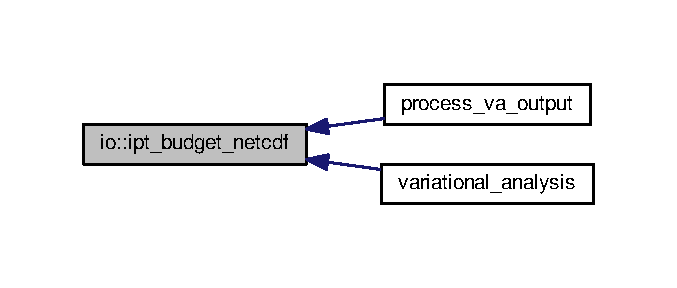
\includegraphics[width=325pt]{namespaceio_aba707a842ac0a3e2e9def20af0b36c32_icgraph}
\end{center}
\end{figure}


\index{io@{io}!ipt\+\_\+ht@{ipt\+\_\+ht}}
\index{ipt\+\_\+ht@{ipt\+\_\+ht}!io@{io}}
\subsubsection[{\texorpdfstring{ipt\+\_\+ht(\+I\+N\+P\+U\+T\+F\+I\+L\+E, I\+N\+S\+T\+R\+U\+M\+E\+N\+T, N\+V, N\+S\+T, N\+T, V, S\+T, L\+O\+N, L\+A\+T, T, D)}{ipt_ht(INPUTFILE, INSTRUMENT, NV, NST, NT, V, ST, LON, LAT, T, D)}}]{\setlength{\rightskip}{0pt plus 5cm}subroutine io\+::ipt\+\_\+ht (
\begin{DoxyParamCaption}
\item[{character (len=$\ast$), intent(in)}]{I\+N\+P\+U\+T\+F\+I\+LE, }
\item[{character (len=64), intent(out)}]{I\+N\+S\+T\+R\+U\+M\+E\+NT, }
\item[{integer (kind=ik4), intent(out)}]{NV, }
\item[{integer (kind=ik4), intent(out)}]{N\+ST, }
\item[{integer (kind=ik4), intent(out)}]{NT, }
\item[{character (len=64), dimension(\+:), intent(out), allocatable}]{V, }
\item[{character (len=64), dimension(\+:), intent(out), allocatable}]{ST, }
\item[{real (kind=rk8), dimension(\+:), intent(out), allocatable}]{L\+ON, }
\item[{real (kind=rk8), dimension(\+:), intent(out), allocatable}]{L\+AT, }
\item[{real (kind=rk8), dimension(\+:), intent(out), allocatable}]{T, }
\item[{real (kind=rk8), dimension(\+:,\+:,\+:), intent(out), allocatable}]{D}
\end{DoxyParamCaption}
)}\hypertarget{namespaceio_ae478b0148dea487c688bfea00e08cade}{}\label{namespaceio_ae478b0148dea487c688bfea00e08cade}


Definition at line 163 of file io.\+f90.


\begin{DoxyCode}
163     \textcolor{keywordtype}{USE }\hyperlink{namespaceportable}{portable}
164 
165     \textcolor{keywordtype}{IMPLICIT NONE}
166 
167     \textcolor{keywordtype}{CHARACTER (LEN=*)}, \textcolor{keywordtype}{INTENT(IN)}                                       :: inputfile    \textcolor{comment}{! Input data
       filename.}
168     \textcolor{keywordtype}{CHARACTER (LEN=64)}, \textcolor{keywordtype}{INTENT(OUT)}                                     :: instrument   \textcolor{comment}{! Name of
       instrument which created the data.}
169     \textcolor{keywordtype}{INTEGER (KIND=IK4)}, \textcolor{keywordtype}{INTENT(OUT)}                                     :: nv           \textcolor{comment}{! Number of
       variables?}
170     \textcolor{keywordtype}{INTEGER (KIND=IK4)}, \textcolor{keywordtype}{INTENT(OUT)}                                     :: nst          \textcolor{comment}{! Number of
       stations.}
171     \textcolor{keywordtype}{INTEGER (KIND=IK4)}, \textcolor{keywordtype}{INTENT(OUT)}                                     :: nt           \textcolor{comment}{! Number of time
       steps.}
172     \textcolor{keywordtype}{CHARACTER (LEN=64)}, \textcolor{keywordtype}{DIMENSION(:)}, \textcolor{keywordtype}{ALLOCATABLE}, \textcolor{keywordtype}{INTENT(OUT)}          :: v            \textcolor{comment}{! Names of the
       variables.}
173     \textcolor{keywordtype}{CHARACTER (LEN=64)}, \textcolor{keywordtype}{DIMENSION(:)}, \textcolor{keywordtype}{ALLOCATABLE}, \textcolor{keywordtype}{INTENT(OUT)}          :: st           \textcolor{comment}{! Names of the
       stations.}
174     \textcolor{keywordtype}{REAL (KIND=RK8)}, \textcolor{keywordtype}{DIMENSION(:)}, \textcolor{keywordtype}{ALLOCATABLE}, \textcolor{keywordtype}{INTENT(OUT)}             :: lon          \textcolor{comment}{! Longitudes of the
       stations.}
175     \textcolor{keywordtype}{REAL (KIND=RK8)}, \textcolor{keywordtype}{DIMENSION(:)}, \textcolor{keywordtype}{ALLOCATABLE}, \textcolor{keywordtype}{INTENT(OUT)}             :: lat          \textcolor{comment}{! Latitudes of the
       stations.}
176     \textcolor{keywordtype}{REAL (KIND=RK8)}, \textcolor{keywordtype}{DIMENSION(:)}, \textcolor{keywordtype}{ALLOCATABLE}, \textcolor{keywordtype}{INTENT(OUT)}             :: t            \textcolor{comment}{! Time steps.}
177     \textcolor{keywordtype}{REAL (KIND=RK8)}, \textcolor{keywordtype}{DIMENSION(:,:,:)}, \textcolor{keywordtype}{ALLOCATABLE}, \textcolor{keywordtype}{INTENT(OUT)}         :: d            \textcolor{comment}{! The data.}
178 
179     \textcolor{comment}{!}
180     \textcolor{comment}{! Local variables.}
181     \textcolor{comment}{!}
182     \textcolor{keywordtype}{INTEGER (KIND=IK4)}                                                  :: iost         \textcolor{comment}{! Status of IO
       operations.}
183     \textcolor{keywordtype}{INTEGER (KIND=IK4)}                                                  :: memst        \textcolor{comment}{! Status of memory
       allocation operations.}
184     \textcolor{keywordtype}{INTEGER (KIND=IK4)}                                                  :: ii, jj, kk   \textcolor{comment}{! Counters.}
185 
186     iost    = 0
187     print *,\textcolor{stringliteral}{'I: Reading data from '},inputfile
188 
189     \textcolor{comment}{!}
190     \textcolor{comment}{! Open the data file. Be cautious, and don't let the file be written to.}
191     \textcolor{comment}{!}
192     \textcolor{keyword}{OPEN} (unit=100, iostat=iost, err=9999, file=inputfile, status=\textcolor{stringliteral}{'OLD'}, access=\textcolor{stringliteral}{'SEQUENTIAL'}, form=\textcolor{stringliteral}{
      'FORMATTED'}, action=\textcolor{stringliteral}{'READ'})
193 
194     \textcolor{comment}{!}
195     \textcolor{comment}{! Read the file headers.}
196     \textcolor{comment}{!}
197     \textcolor{keyword}{READ} (fmt=\textcolor{stringliteral}{'(A64)'}, unit=100, err=9999, iostat=iost) instrument         \textcolor{comment}{! Name of the instrument
       producing the data.}
198     \textcolor{keyword}{READ} (fmt=\textcolor{stringliteral}{'(I6)'}, unit=100, err=9999, iostat=iost) nv                  \textcolor{comment}{! Number of variables.}
199     \textcolor{keyword}{READ} (fmt=\textcolor{stringliteral}{'(I6)'}, unit=100, err=9999, iostat=iost) nst                 \textcolor{comment}{! Number of stations.}
200     \textcolor{keyword}{READ} (fmt=\textcolor{stringliteral}{'(I6)'}, unit=100, err=9999, iostat=iost) nt                  \textcolor{comment}{! Number of time steps.}
201 
202     \textcolor{comment}{!}
203     \textcolor{comment}{! Allocate enough space in the data arrays. We might as well be paranoid, and check if the arrays have
       already been}
204     \textcolor{comment}{! allocated (and if so, deallocate them).}
205     \textcolor{comment}{!}
206     \textcolor{keywordflow}{IF} (\textcolor{keyword}{ALLOCATED}(v))   \textcolor{keyword}{DEALLOCATE}(v)
207     \textcolor{keywordflow}{IF} (\textcolor{keyword}{ALLOCATED}(st))  \textcolor{keyword}{DEALLOCATE}(st)
208     \textcolor{keywordflow}{IF} (\textcolor{keyword}{ALLOCATED}(lon)) \textcolor{keyword}{DEALLOCATE}(lon)
209     \textcolor{keywordflow}{IF} (\textcolor{keyword}{ALLOCATED}(lat)) \textcolor{keyword}{DEALLOCATE}(lat)
210     \textcolor{keywordflow}{IF} (\textcolor{keyword}{ALLOCATED}(d))   \textcolor{keyword}{DEALLOCATE}(d)
211 
212     \textcolor{keyword}{ALLOCATE}(v(nv), st(nst), lon(nst), lat(nst), t(nt), d(nv,nst,nt), stat=memst)
213     \textcolor{keywordflow}{IF} (memst .NE. 0) \textcolor{keywordflow}{THEN}
214         print *,\textcolor{stringliteral}{'E: Unable to allocate memory to hold 2D data'}
215         stop \textcolor{stringliteral}{'1'}
216 \textcolor{keywordflow}{    END IF}
217 
218     \textcolor{comment}{!}
219     \textcolor{comment}{! Read the data arrays.}
220     \textcolor{comment}{!}
221     \textcolor{keyword}{READ} (fmt=\textcolor{stringliteral}{'(A64)'}, unit=100, err=9999, iostat=iost) (v(ii), ii=1,nv)       \textcolor{comment}{! Read the variable names.}
222     \textcolor{keyword}{READ} (fmt=\textcolor{stringliteral}{'(A64)'}, unit=100, err=9999, iostat=iost) (st(ii), ii=1,nst)     \textcolor{comment}{! Read the station names.}
223     \textcolor{keyword}{READ} (fmt=\textcolor{stringliteral}{'(F10.5)'}, unit=100, err=9999, iostat=iost) (lon(ii), ii=1,nst)  \textcolor{comment}{! Read the station
       longitudes.}
224     \textcolor{keyword}{READ} (fmt=\textcolor{stringliteral}{'(F10.5)'}, unit=100, err=9999, iostat=iost) (lat(ii), ii=1,nst)  \textcolor{comment}{! Read the station
       latitudes.}
225     \textcolor{keyword}{READ} (fmt=\textcolor{stringliteral}{'(F10.5)'}, unit=100, err=9999, iostat=iost) (t(ii), ii=1,nt)     \textcolor{comment}{! Read the times.}
226 
227     \textcolor{comment}{!}
228     \textcolor{comment}{! Read all the data. Don't know how (or if) this can be done with an implicit do loop, therefore will
       do it the old fashioned}
229     \textcolor{comment}{! way.}
230     \textcolor{comment}{!}
231     \textcolor{keywordflow}{DO} kk=1,nt
232         \textcolor{keywordflow}{DO} jj=1,nst
233             \textcolor{keywordflow}{DO} ii=1,nv
234                 \textcolor{keyword}{READ}(fmt=\textcolor{stringliteral}{'(F10.3)'}, unit=100, err=9999, iostat=iost) d(ii,jj,kk)
235 \textcolor{keywordflow}{            END DO}
236 \textcolor{keywordflow}{        END DO}
237 \textcolor{keywordflow}{    END DO}
238 
239     \textcolor{comment}{!}
240     \textcolor{comment}{! Close the data file.}
241     \textcolor{comment}{!}
242     \textcolor{keyword}{CLOSE} (unit=100, err=9999, iostat=iost, status=\textcolor{stringliteral}{'KEEP'})
243 
244     \textcolor{comment}{!}
245     \textcolor{comment}{! The next block of code deals with IO errors (if they occurred).}
246     \textcolor{comment}{!}
247     9999 \textcolor{keywordflow}{CONTINUE}
248     \textcolor{keywordflow}{IF} (iost .GT. 0) \textcolor{keywordflow}{THEN}
249         print *,\textcolor{stringliteral}{'E: An IO error occurred while reading '},inputfile
250         stop \textcolor{stringliteral}{'1'}
251 \textcolor{keywordflow}{    END IF}
252 
\end{DoxyCode}


Here is the caller graph for this function\+:\nopagebreak
\begin{figure}[H]
\begin{center}
\leavevmode
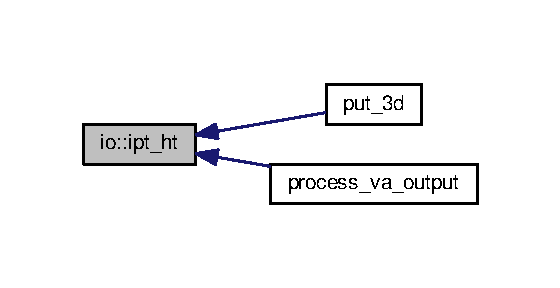
\includegraphics[width=269pt]{namespaceio_ae478b0148dea487c688bfea00e08cade_icgraph}
\end{center}
\end{figure}


\index{io@{io}!ipt\+\_\+vht@{ipt\+\_\+vht}}
\index{ipt\+\_\+vht@{ipt\+\_\+vht}!io@{io}}
\subsubsection[{\texorpdfstring{ipt\+\_\+vht(\+I\+N\+P\+U\+T\+F\+I\+L\+E, I\+N\+S\+T\+R\+U\+M\+E\+N\+T, N\+V, N\+P, N\+S\+T, N\+T, V, P, S\+T, T, D)}{ipt_vht(INPUTFILE, INSTRUMENT, NV, NP, NST, NT, V, P, ST, T, D)}}]{\setlength{\rightskip}{0pt plus 5cm}subroutine io\+::ipt\+\_\+vht (
\begin{DoxyParamCaption}
\item[{character (len=$\ast$), intent(in)}]{I\+N\+P\+U\+T\+F\+I\+LE, }
\item[{character (len=64), intent(out)}]{I\+N\+S\+T\+R\+U\+M\+E\+NT, }
\item[{integer (kind=ik4), intent(out)}]{NV, }
\item[{integer (kind=ik4), intent(out)}]{NP, }
\item[{integer (kind=ik4), intent(out)}]{N\+ST, }
\item[{integer (kind=ik4), intent(out)}]{NT, }
\item[{character (len=64), dimension(\+:), intent(out), allocatable}]{V, }
\item[{real (kind=rk8), dimension(\+:), intent(out), allocatable}]{P, }
\item[{character (len=64), dimension(\+:), intent(out), allocatable}]{ST, }
\item[{real (kind=rk8), dimension(\+:), intent(out), allocatable}]{T, }
\item[{real (kind=rk8), dimension(\+:,\+:,\+:,\+:), intent(out), allocatable}]{D}
\end{DoxyParamCaption}
)}\hypertarget{namespaceio_abed61f2af0a37265b7a1d15300f61996}{}\label{namespaceio_abed61f2af0a37265b7a1d15300f61996}


Definition at line 46 of file io.\+f90.


\begin{DoxyCode}
46     \textcolor{keywordtype}{USE }\hyperlink{namespaceportable}{portable}
47 
48     \textcolor{keywordtype}{IMPLICIT NONE}
49     \textcolor{keywordtype}{CHARACTER (LEN=*)}, \textcolor{keywordtype}{INTENT(IN)}                                       :: inputfile    \textcolor{comment}{! Name of the input
       file.}
50     \textcolor{keywordtype}{CHARACTER (LEN=64)}, \textcolor{keywordtype}{INTENT(OUT)}                                     :: instrument   \textcolor{comment}{! Instrument name.}
51     \textcolor{keywordtype}{INTEGER (KIND=IK4)}, \textcolor{keywordtype}{INTENT(OUT)}                                     :: nv           \textcolor{comment}{! Number of
       variables?}
52     \textcolor{keywordtype}{INTEGER (KIND=IK4)}, \textcolor{keywordtype}{INTENT(OUT)}                                     :: np           \textcolor{comment}{! Number of
       pressure levels.}
53     \textcolor{keywordtype}{INTEGER (KIND=IK4)}, \textcolor{keywordtype}{INTENT(OUT)}                                     :: nst          \textcolor{comment}{! Number of
       stations.}
54     \textcolor{keywordtype}{INTEGER (KIND=IK4)}, \textcolor{keywordtype}{INTENT(OUT)}                                     :: nt           \textcolor{comment}{! Number of time
       steps.}
55     \textcolor{keywordtype}{CHARACTER (LEN=64)}, \textcolor{keywordtype}{DIMENSION(:)}, \textcolor{keywordtype}{ALLOCATABLE}, \textcolor{keywordtype}{INTENT(OUT)}          :: v            \textcolor{comment}{! Variable names?}
56     \textcolor{keywordtype}{REAL (KIND=RK8)}, \textcolor{keywordtype}{DIMENSION(:)}, \textcolor{keywordtype}{ALLOCATABLE}, \textcolor{keywordtype}{INTENT(OUT)}             :: p            \textcolor{comment}{! Values of the
       pressure levels.}
57     \textcolor{keywordtype}{CHARACTER (LEN=64)}, \textcolor{keywordtype}{DIMENSION(:)}, \textcolor{keywordtype}{ALLOCATABLE}, \textcolor{keywordtype}{INTENT(OUT)}          :: st           \textcolor{comment}{! Station names?}
58     \textcolor{keywordtype}{REAL (KIND=RK8)}, \textcolor{keywordtype}{DIMENSION(:)}, \textcolor{keywordtype}{ALLOCATABLE}, \textcolor{keywordtype}{INTENT(OUT)}             :: t            \textcolor{comment}{! Time values?}
59     \textcolor{keywordtype}{REAL (KIND=RK8)}, \textcolor{keywordtype}{DIMENSION(:,:,:,:)}, \textcolor{keywordtype}{ALLOCATABLE}, \textcolor{keywordtype}{INTENT(OUT)}       :: d            \textcolor{comment}{! The data.}
60 
61     \textcolor{comment}{!}
62     \textcolor{comment}{! Local variables.}
63     \textcolor{comment}{!}
64     \textcolor{keywordtype}{INTEGER (KIND=IK4)}                                                  :: iost         \textcolor{comment}{! IO status (0 (OK)
       or +ve (error))}
65     \textcolor{keywordtype}{INTEGER (KIND=IK4)}                                                  :: memst        \textcolor{comment}{! Status from
       ALLOCATE commands.}
66     \textcolor{keywordtype}{INTEGER (KIND=IK4)}                                                  :: ii,jj,kk,ll  \textcolor{comment}{! Counters}
67 
68     iost = 0
69     print *,\textcolor{stringliteral}{'I: Reading data from '},inputfile
70 
71     \textcolor{comment}{!}
72     \textcolor{comment}{! Open the data file. Be cautious, and don't let the file be written to.}
73     \textcolor{comment}{!}
74     \textcolor{keyword}{OPEN} (unit=100, iostat=iost, err=9999, file=inputfile, status=\textcolor{stringliteral}{'OLD'}, access=\textcolor{stringliteral}{'SEQUENTIAL'}, form=\textcolor{stringliteral}{
      'FORMATTED'}, action=\textcolor{stringliteral}{'READ'})
75 
76     \textcolor{comment}{!}
77     \textcolor{comment}{! Read the file headers.}
78     \textcolor{comment}{!}
79     \textcolor{keyword}{READ} (fmt=\textcolor{stringliteral}{'(A64)'}, unit=100, err=9999, iostat=iost) instrument         \textcolor{comment}{! Name of the instrument
       producing the data.}
80     \textcolor{keyword}{READ} (fmt=\textcolor{stringliteral}{'(I6)'}, unit=100, err=9999, iostat=iost) nv                  \textcolor{comment}{! Number of variables.}
81     \textcolor{keyword}{READ} (fmt=\textcolor{stringliteral}{'(I6)'}, unit=100, err=9999, iostat=iost) np                  \textcolor{comment}{! Number of pressure levels.}
82     \textcolor{keyword}{READ} (fmt=\textcolor{stringliteral}{'(I6)'}, unit=100, err=9999, iostat=iost) nst                 \textcolor{comment}{! Number of stations.}
83     \textcolor{keyword}{READ} (fmt=\textcolor{stringliteral}{'(I6)'}, unit=100, err=9999, iostat=iost) nt                  \textcolor{comment}{! Number of time steps.}
84 
85     \textcolor{comment}{!}
86     \textcolor{comment}{! Allocate enough space in the data arrays. We might as well be paranoid, and check if the arrays have
       already been}
87     \textcolor{comment}{! allocated (and if so, deallocate them).}
88     \textcolor{comment}{!}
89     \textcolor{keywordflow}{IF} (\textcolor{keyword}{ALLOCATED}(v))   \textcolor{keyword}{DEALLOCATE}(v)
90     \textcolor{keywordflow}{IF} (\textcolor{keyword}{ALLOCATED}(p))   \textcolor{keyword}{DEALLOCATE}(p)
91     \textcolor{keywordflow}{IF} (\textcolor{keyword}{ALLOCATED}(st))  \textcolor{keyword}{DEALLOCATE}(st)
92     \textcolor{keywordflow}{IF} (\textcolor{keyword}{ALLOCATED}(t))   \textcolor{keyword}{DEALLOCATE}(t)
93     \textcolor{keywordflow}{IF} (\textcolor{keyword}{ALLOCATED}(d))   \textcolor{keyword}{DEALLOCATE}(d)
94 
95     \textcolor{keyword}{ALLOCATE}(v(nv), p(np), st(nst), t(nt), d(nv,np,nst,nt), stat=memst)
96     \textcolor{keywordflow}{IF} (memst .NE. 0) \textcolor{keywordflow}{THEN}
97         print *,\textcolor{stringliteral}{'E: Unable to allocate memory to hold 3D data'}
98         stop \textcolor{stringliteral}{'1'}
99 \textcolor{keywordflow}{    END IF}
100 
101     \textcolor{comment}{!}
102     \textcolor{comment}{! Read the data arrays.}
103     \textcolor{comment}{!}
104     \textcolor{keyword}{READ} (fmt=\textcolor{stringliteral}{'(A64)'}, unit=100, err=9999, iostat=iost) (v(ii), ii=1,nv)       \textcolor{comment}{! Read the variable names.}
105     \textcolor{keyword}{READ} (fmt=\textcolor{stringliteral}{'(F7.2)'}, unit=100, err=9999, iostat=iost) (p(ii), ii=1,np)      \textcolor{comment}{! Read the pressure levels.}
106     \textcolor{keyword}{READ} (fmt=\textcolor{stringliteral}{'(A64)'}, unit=100, err=9999, iostat=iost) (st(ii), ii=1,nst)     \textcolor{comment}{! Read the station names.}
107     \textcolor{keyword}{READ} (fmt=\textcolor{stringliteral}{'(F10.5)'}, unit=100, err=9999, iostat=iost) (t(ii), ii=1,nt)     \textcolor{comment}{! Read the times.}
108 
109     \textcolor{comment}{!}
110     \textcolor{comment}{! Read all the data. Don't know how (or if) this can be done with an implicit do loop, therefore will
       do it the old fashioned}
111     \textcolor{comment}{! way.}
112     \textcolor{comment}{!}
113     \textcolor{keywordflow}{DO} ll=1,nt
114         \textcolor{keywordflow}{DO} kk=1,nst
115             \textcolor{keywordflow}{DO} jj=1,np
116                 \textcolor{keywordflow}{DO} ii=1,nv
117                     \textcolor{keyword}{READ}(fmt=\textcolor{stringliteral}{'(F10.3)'}, unit=100, err=9999, iostat=iost) d(ii,jj,kk,ll)
118 \textcolor{keywordflow}{                END DO}
119 \textcolor{keywordflow}{            END DO}
120 \textcolor{keywordflow}{        END DO}
121 \textcolor{keywordflow}{    END DO}
122 
123     \textcolor{comment}{!}
124     \textcolor{comment}{! Close the data file.}
125     \textcolor{comment}{!}
126     \textcolor{keyword}{CLOSE} (unit=100, err=9999, iostat=iost, status=\textcolor{stringliteral}{'KEEP'})
127 
128     \textcolor{comment}{!}
129     \textcolor{comment}{! The next block of code deals with IO errors (if they occurred).}
130     \textcolor{comment}{!}
131     9999 \textcolor{keywordflow}{CONTINUE}
132     \textcolor{keywordflow}{IF} (iost .GT. 0) \textcolor{keywordflow}{THEN}
133         print *,\textcolor{stringliteral}{'E: An IO error occurred while reading '},inputfile
134         stop \textcolor{stringliteral}{'1'}
135 \textcolor{keywordflow}{    END IF}
136 
\end{DoxyCode}


Here is the caller graph for this function\+:\nopagebreak
\begin{figure}[H]
\begin{center}
\leavevmode
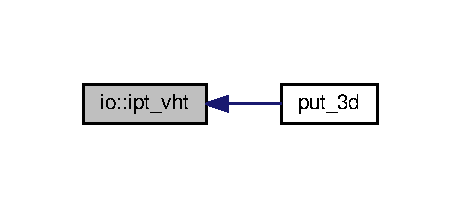
\includegraphics[width=221pt]{namespaceio_abed61f2af0a37265b7a1d15300f61996_icgraph}
\end{center}
\end{figure}


\index{io@{io}!opt\+\_\+2d\+\_\+netcdf@{opt\+\_\+2d\+\_\+netcdf}}
\index{opt\+\_\+2d\+\_\+netcdf@{opt\+\_\+2d\+\_\+netcdf}!io@{io}}
\subsubsection[{\texorpdfstring{opt\+\_\+2d\+\_\+netcdf(\+O\+U\+T\+P\+U\+T\+F\+I\+L\+E, T, B\+A\+R\+\_\+\+P\+R\+E\+S, A\+D\+P\+S, P\+R\+E\+C\+I\+P, L\+P\+R\+E\+C\+I\+P, E\+V\+A\+P\+O\+R, S\+H\+F, R\+L, R\+A\+D\+I\+A\+T\+I\+O\+N\+T, R\+A\+D\+I\+A\+T\+I\+O\+N\+B, R\+A\+D\+I\+A\+T\+I\+O\+N, T\+A\+O\+X, T\+A\+O\+Y)}{opt_2d_netcdf(OUTPUTFILE, T, BAR_PRES, ADPS, PRECIP, LPRECIP, EVAPOR, SHF, RL, RADIATIONT, RADIATIONB, RADIATION, TAOX, TAOY)}}]{\setlength{\rightskip}{0pt plus 5cm}subroutine io\+::opt\+\_\+2d\+\_\+netcdf (
\begin{DoxyParamCaption}
\item[{character (len=$\ast$), intent(in)}]{O\+U\+T\+P\+U\+T\+F\+I\+LE, }
\item[{real (kind=rk8), dimension(\+:), intent(in)}]{T, }
\item[{real (kind=rk8), dimension(\+:), intent(in)}]{B\+A\+R\+\_\+\+P\+R\+ES, }
\item[{real (kind=rk8), dimension(\+:), intent(in)}]{A\+D\+PS, }
\item[{real (kind=rk8), dimension(\+:), intent(in)}]{P\+R\+E\+C\+IP, }
\item[{real (kind=rk8), dimension(\+:), intent(in)}]{L\+P\+R\+E\+C\+IP, }
\item[{real (kind=rk8), dimension(\+:), intent(in)}]{E\+V\+A\+P\+OR, }
\item[{real (kind=rk8), dimension(\+:), intent(in)}]{S\+HF, }
\item[{real (kind=rk8), dimension(\+:), intent(in)}]{RL, }
\item[{real (kind=rk8), dimension(\+:), intent(in)}]{R\+A\+D\+I\+A\+T\+I\+O\+NT, }
\item[{real (kind=rk8), dimension(\+:), intent(in)}]{R\+A\+D\+I\+A\+T\+I\+O\+NB, }
\item[{real (kind=rk8), dimension(\+:), intent(in)}]{R\+A\+D\+I\+A\+T\+I\+ON, }
\item[{real (kind=rk8), dimension(\+:), intent(in)}]{T\+A\+OX, }
\item[{real (kind=rk8), dimension(\+:), intent(in)}]{T\+A\+OY}
\end{DoxyParamCaption}
)}\hypertarget{namespaceio_ab6bcb3dc7b4a08b242b7fbd4e11ed319}{}\label{namespaceio_ab6bcb3dc7b4a08b242b7fbd4e11ed319}


Definition at line 1287 of file io.\+f90.


\begin{DoxyCode}
1287     \textcolor{keywordtype}{USE }\hyperlink{namespaceportable}{portable}
1288     \textcolor{keywordtype}{USE }netcdf
1289 
1290     \textcolor{keywordtype}{IMPLICIT NONE}
1291 
1292     \textcolor{keywordtype}{CHARACTER (LEN=*)}, \textcolor{keywordtype}{INTENT(IN)}                                       :: outputfile   \textcolor{comment}{! Name of the
       output file.}
1293     \textcolor{keywordtype}{REAL (KIND=RK8)}, \textcolor{keywordtype}{DIMENSION(:)}, \textcolor{keywordtype}{INTENT(IN)}                           :: t            \textcolor{comment}{! Time.}
1294     \textcolor{keywordtype}{REAL (KIND=RK8)}, \textcolor{keywordtype}{DIMENSION(:)}, \textcolor{keywordtype}{INTENT(IN)}                           :: bar\_pres     \textcolor{comment}{! Barometric
       pressure (hPa).}
1295     \textcolor{keywordtype}{REAL (KIND=RK8)}, \textcolor{keywordtype}{DIMENSION(:)}, \textcolor{keywordtype}{INTENT(IN)}                           :: adps         \textcolor{comment}{! V.grad(PS)}
1296     \textcolor{keywordtype}{REAL (KIND=RK8)}, \textcolor{keywordtype}{DIMENSION(:)}, \textcolor{keywordtype}{INTENT(IN)}                           :: precip
1297     \textcolor{keywordtype}{REAL (KIND=RK8)}, \textcolor{keywordtype}{DIMENSION(:)}, \textcolor{keywordtype}{INTENT(IN)}                           :: lprecip
1298     \textcolor{keywordtype}{REAL (KIND=RK8)}, \textcolor{keywordtype}{DIMENSION(:)}, \textcolor{keywordtype}{INTENT(IN)}                           :: evapor
1299     \textcolor{keywordtype}{REAL (KIND=RK8)}, \textcolor{keywordtype}{DIMENSION(:)}, \textcolor{keywordtype}{INTENT(IN)}                           :: shf
1300     \textcolor{keywordtype}{REAL (KIND=RK8)}, \textcolor{keywordtype}{DIMENSION(:)}, \textcolor{keywordtype}{INTENT(IN)}                           :: rl
1301     \textcolor{keywordtype}{REAL (KIND=RK8)}, \textcolor{keywordtype}{DIMENSION(:)}, \textcolor{keywordtype}{INTENT(IN)}                           :: radiationt
1302     \textcolor{keywordtype}{REAL (KIND=RK8)}, \textcolor{keywordtype}{DIMENSION(:)}, \textcolor{keywordtype}{INTENT(IN)}                           :: radiationb
1303     \textcolor{keywordtype}{REAL (KIND=RK8)}, \textcolor{keywordtype}{DIMENSION(:)}, \textcolor{keywordtype}{INTENT(IN)}                           :: radiation
1304     \textcolor{keywordtype}{REAL (KIND=RK8)}, \textcolor{keywordtype}{DIMENSION(:)}, \textcolor{keywordtype}{INTENT(IN)}                           :: taox
1305     \textcolor{keywordtype}{REAL (KIND=RK8)}, \textcolor{keywordtype}{DIMENSION(:)}, \textcolor{keywordtype}{INTENT(IN)}                           :: taoy
1306 
1307     \textcolor{comment}{!}
1308     \textcolor{comment}{! Local variables.}
1309     \textcolor{comment}{!}
1310     \textcolor{keywordtype}{INTEGER (KIND=IK4)}          :: ncid                                                 \textcolor{comment}{! ID of NetCDF
       file.}
1311     \textcolor{keywordtype}{INTEGER (KIND=IK4)}          :: t\_dim\_id                                             \textcolor{comment}{! Time dimension
       ID.}
1312     \textcolor{keywordtype}{INTEGER (KIND=IK4)}          :: t\_var\_id                                             \textcolor{comment}{! Time coordinate
       variable.}
1313     \textcolor{keywordtype}{INTEGER (KIND=IK4)}          :: bar\_pres\_var\_id
1314     \textcolor{keywordtype}{INTEGER (KIND=IK4)}          :: adps\_var\_id
1315     \textcolor{keywordtype}{INTEGER (KIND=IK4)}          :: precip\_var\_id
1316     \textcolor{keywordtype}{INTEGER (KIND=IK4)}          :: lprecip\_var\_id
1317     \textcolor{keywordtype}{INTEGER (KIND=IK4)}          :: evapor\_var\_id
1318     \textcolor{keywordtype}{INTEGER (KIND=IK4)}          :: shf\_var\_id
1319     \textcolor{keywordtype}{INTEGER (KIND=IK4)}          :: rl\_var\_id
1320     \textcolor{keywordtype}{INTEGER (KIND=IK4)}          :: radiationt\_var\_id
1321     \textcolor{keywordtype}{INTEGER (KIND=IK4)}          :: radiationb\_var\_id
1322     \textcolor{keywordtype}{INTEGER (KIND=IK4)}          :: radiation\_var\_id
1323     \textcolor{keywordtype}{INTEGER (KIND=IK4)}          :: taox\_var\_id
1324     \textcolor{keywordtype}{INTEGER (KIND=IK4)}          :: taoy\_var\_id
1325     \textcolor{keywordtype}{INTEGER (KIND=IK4)}          :: iost                                                 \textcolor{comment}{! I/O status.}
1326     \textcolor{keywordtype}{LOGICAL}                     :: ncerror                                               \textcolor{comment}{! Did a NetCDF
       function fail?}
1327 
1328     iost    = nf90\_noerr
1329     ncerror = .false.
1330     \textcolor{comment}{!}
1331     \textcolor{comment}{! Create the NetCDF file.}
1332     \textcolor{comment}{!}
1333     iost    = nf90\_create(outputfile, nf90\_noclobber, ncid)
1334     \textcolor{keywordflow}{IF} (iost .NE. nf90\_noerr) \textcolor{keywordflow}{GO TO} 9999
1335 
1336     \textcolor{comment}{!}
1337     \textcolor{comment}{! Define the dimensions.}
1338     \textcolor{comment}{!}
1339     iost    = nf90\_def\_dim(ncid, \textcolor{stringliteral}{"time"}, \textcolor{keyword}{SIZE}(t), t\_dim\_id)                          \textcolor{comment}{! Time steps.}
1340     \textcolor{keywordflow}{IF} (iost .NE. nf90\_noerr) \textcolor{keywordflow}{GO TO} 9999
1341 
1342     \textcolor{comment}{!}
1343     \textcolor{comment}{! Define the variables.}
1344     \textcolor{comment}{!}
1345     ncerror = .false.
1346     ncerror = (nf90\_def\_var(ncid, \textcolor{stringliteral}{"time"}, nf90\_double, (/ t\_dim\_id /), t\_var\_id)                    .NE. 
      nf90\_noerr)
1347     ncerror = (nf90\_def\_var(ncid, \textcolor{stringliteral}{"bar\_pres"}, nf90\_double, (/ t\_dim\_id /), bar\_pres\_var\_id)         .NE. 
      nf90\_noerr) .OR. ncerror
1348     ncerror = (nf90\_def\_var(ncid, \textcolor{stringliteral}{"adps"}, nf90\_double, (/ t\_dim\_id /), adps\_var\_id)                 .NE. 
      nf90\_noerr) .OR. ncerror
1349     ncerror = (nf90\_def\_var(ncid, \textcolor{stringliteral}{"precip"}, nf90\_double, (/ t\_dim\_id /), precip\_var\_id)             .NE. 
      nf90\_noerr) .OR. ncerror
1350     ncerror = (nf90\_def\_var(ncid, \textcolor{stringliteral}{"lprecip"}, nf90\_double, (/ t\_dim\_id /), lprecip\_var\_id)           .NE. 
      nf90\_noerr) .OR. ncerror
1351     ncerror = (nf90\_def\_var(ncid, \textcolor{stringliteral}{"evapor"}, nf90\_double, (/ t\_dim\_id /), evapor\_var\_id)             .NE. 
      nf90\_noerr) .OR. ncerror
1352     ncerror = (nf90\_def\_var(ncid, \textcolor{stringliteral}{"shf"}, nf90\_double, (/ t\_dim\_id /), shf\_var\_id)                   .NE. 
      nf90\_noerr) .OR. ncerror
1353     ncerror = (nf90\_def\_var(ncid, \textcolor{stringliteral}{"rl"}, nf90\_double, (/ t\_dim\_id /), rl\_var\_id)                     .NE. 
      nf90\_noerr) .OR. ncerror
1354     ncerror = (nf90\_def\_var(ncid, \textcolor{stringliteral}{"radiationt"}, nf90\_double, (/ t\_dim\_id /), radiationt\_var\_id)     .NE. 
      nf90\_noerr) .OR. ncerror
1355     ncerror = (nf90\_def\_var(ncid, \textcolor{stringliteral}{"radiationb"}, nf90\_double, (/ t\_dim\_id /), radiationb\_var\_id)     .NE. 
      nf90\_noerr) .OR. ncerror
1356     ncerror = (nf90\_def\_var(ncid, \textcolor{stringliteral}{"radiation"}, nf90\_double, (/ t\_dim\_id /), radiation\_var\_id)       .NE. 
      nf90\_noerr) .OR. ncerror
1357     ncerror = (nf90\_def\_var(ncid, \textcolor{stringliteral}{"taox"}, nf90\_double, (/ t\_dim\_id /), taox\_var\_id)                 .NE. 
      nf90\_noerr) .OR. ncerror
1358     ncerror = (nf90\_def\_var(ncid, \textcolor{stringliteral}{"taoy"}, nf90\_double, (/ t\_dim\_id /), taoy\_var\_id)                 .NE. 
      nf90\_noerr) .OR. ncerror
1359     \textcolor{keywordflow}{IF} (ncerror) \textcolor{keywordflow}{GO TO} 9999
1360 
1361     \textcolor{comment}{!}
1362     \textcolor{comment}{! Create various attributes. Make sure strings are null terminated (for C programs).}
1363     \textcolor{comment}{!}
1364     ncerror = .false.
1365     ncerror = (nf90\_put\_att(ncid, t\_var\_id, \textcolor{stringliteral}{"long\_name"}, \textcolor{stringliteral}{'Time'}//char(0))                           .NE. 
      nf90\_noerr)
1366     ncerror = (nf90\_put\_att(ncid, t\_var\_id, \textcolor{stringliteral}{"units"}, \textcolor{stringliteral}{'Days since 2004-12-31T00:00:00 UTC'}//char(0)) .NE. 
      nf90\_noerr) .OR. ncerror
1367     ncerror = (nf90\_put\_att(ncid, t\_var\_id, \textcolor{stringliteral}{"missing\_value"}, nf90\_fill\_double)                      .NE. 
      nf90\_noerr) .OR. ncerror
1368     ncerror = (nf90\_put\_att(ncid, bar\_pres\_var\_id, \textcolor{stringliteral}{"long\_name"}, \textcolor{stringliteral}{'Barometric pressure'}//char(0))     .NE. 
      nf90\_noerr) .OR. ncerror
1369     ncerror = (nf90\_put\_att(ncid, bar\_pres\_var\_id, \textcolor{stringliteral}{"units"}, \textcolor{stringliteral}{'Pa'}//char(0))                          .NE. 
      nf90\_noerr) .OR. ncerror
1370     ncerror = (nf90\_put\_att(ncid, bar\_pres\_var\_id, \textcolor{stringliteral}{"missing\_value"}, nf90\_fill\_double)               .NE. 
      nf90\_noerr) .OR. ncerror
1371     ncerror = (nf90\_put\_att(ncid, adps\_var\_id, \textcolor{stringliteral}{"long\_name"}, \textcolor{stringliteral}{'V.grad(Ps)'}//char(0))                  .NE. 
      nf90\_noerr) .OR. ncerror
1372     ncerror = (nf90\_put\_att(ncid, adps\_var\_id, \textcolor{stringliteral}{"units"}, \textcolor{stringliteral}{'Pa/s'}//char(0))                            .NE. 
      nf90\_noerr) .OR. ncerror
1373     ncerror = (nf90\_put\_att(ncid, adps\_var\_id, \textcolor{stringliteral}{"missing\_value"}, nf90\_fill\_double)                   .NE. 
      nf90\_noerr) .OR. ncerror
1374     ncerror = (nf90\_put\_att(ncid, precip\_var\_id, \textcolor{stringliteral}{"long\_name"}, \textcolor{stringliteral}{'precip * Lv0/Cpd'}//char(0))          .NE. 
      nf90\_noerr) .OR. ncerror
1375     ncerror = (nf90\_put\_att(ncid, precip\_var\_id, \textcolor{stringliteral}{"units"}, \textcolor{stringliteral}{'K/s'}//char(0))                           .NE. 
      nf90\_noerr) .OR. ncerror
1376     ncerror = (nf90\_put\_att(ncid, precip\_var\_id, \textcolor{stringliteral}{"missing\_value"}, nf90\_fill\_double)                 .NE. 
      nf90\_noerr) .OR. ncerror
1377     ncerror = (nf90\_put\_att(ncid, lprecip\_var\_id, \textcolor{stringliteral}{"long\_name"}, \textcolor{stringliteral}{'precip *Lv/Cpd'}//char(0))           .NE. 
      nf90\_noerr) .OR. ncerror
1378     ncerror = (nf90\_put\_att(ncid, lprecip\_var\_id, \textcolor{stringliteral}{"units"}, \textcolor{stringliteral}{'K/s'}//char(0))                          .NE. 
      nf90\_noerr) .OR. ncerror
1379     ncerror = (nf90\_put\_att(ncid, lprecip\_var\_id, \textcolor{stringliteral}{"missing\_value"}, nf90\_fill\_double)                .NE. 
      nf90\_noerr) .OR. ncerror
1380     ncerror = (nf90\_put\_att(ncid, evapor\_var\_id, \textcolor{stringliteral}{"long\_name"}, \textcolor{stringliteral}{'Evaporation * Lv0/Cpd'}//char(0))     .NE. 
      nf90\_noerr) .OR. ncerror
1381     ncerror = (nf90\_put\_att(ncid, evapor\_var\_id, \textcolor{stringliteral}{"units"}, \textcolor{stringliteral}{'K/s'}//char(0))                           .NE. 
      nf90\_noerr) .OR. ncerror
1382     ncerror = (nf90\_put\_att(ncid, evapor\_var\_id, \textcolor{stringliteral}{"missing\_value"}, nf90\_fill\_double)                 .NE. 
      nf90\_noerr) .OR. ncerror
1383     ncerror = (nf90\_put\_att(ncid, shf\_var\_id, \textcolor{stringliteral}{"long\_name"}, \textcolor{stringliteral}{'Sensible heating rate'}//char(0))        .NE. 
      nf90\_noerr) .OR. ncerror
1384     ncerror = (nf90\_put\_att(ncid, shf\_var\_id, \textcolor{stringliteral}{"units"}, \textcolor{stringliteral}{'K/s'}//char(0))                              .NE. 
      nf90\_noerr) .OR. ncerror
1385     ncerror = (nf90\_put\_att(ncid, shf\_var\_id, \textcolor{stringliteral}{"missing\_value"}, nf90\_fill\_double)                    .NE. 
      nf90\_noerr) .OR. ncerror
1386     ncerror = (nf90\_put\_att(ncid, rl\_var\_id, \textcolor{stringliteral}{"long\_name"}, \textcolor{stringliteral}{'Rl * Lv0/Cpd'}//char(0))                  .NE. 
      nf90\_noerr) .OR. ncerror
1387     ncerror = (nf90\_put\_att(ncid, rl\_var\_id, \textcolor{stringliteral}{"units"}, \textcolor{stringliteral}{'K/s'}//char(0))                               .NE. 
      nf90\_noerr) .OR. ncerror
1388     ncerror = (nf90\_put\_att(ncid, rl\_var\_id, \textcolor{stringliteral}{"missing\_value"}, nf90\_fill\_double)                     .NE. 
      nf90\_noerr) .OR. ncerror
1389     ncerror = (nf90\_put\_att(ncid, radiationt\_var\_id, \textcolor{stringliteral}{"long\_name"}, \textcolor{stringliteral}{'Radiative heating-TOA'}//char(0)) .NE. 
      nf90\_noerr) .OR. ncerror
1390     ncerror = (nf90\_put\_att(ncid, radiationt\_var\_id, \textcolor{stringliteral}{"units"}, \textcolor{stringliteral}{'K/s'}//char(0))                       .NE. 
      nf90\_noerr) .OR. ncerror
1391     ncerror = (nf90\_put\_att(ncid, radiationt\_var\_id, \textcolor{stringliteral}{"missing\_value"}, nf90\_fill\_double)             .NE. 
      nf90\_noerr) .OR. ncerror
1392     ncerror = (nf90\_put\_att(ncid, radiationb\_var\_id, \textcolor{stringliteral}{"long\_name"}, \textcolor{stringliteral}{'Radiative heating-SFC'}//char(0)) .NE. 
      nf90\_noerr) .OR. ncerror
1393     ncerror = (nf90\_put\_att(ncid, radiationb\_var\_id, \textcolor{stringliteral}{"units"}, \textcolor{stringliteral}{'K/s'}//char(0))                       .NE. 
      nf90\_noerr) .OR. ncerror
1394     ncerror = (nf90\_put\_att(ncid, radiationb\_var\_id, \textcolor{stringliteral}{"missing\_value"}, nf90\_fill\_double)             .NE. 
      nf90\_noerr) .OR. ncerror
1395     ncerror = (nf90\_put\_att(ncid, radiation\_var\_id, \textcolor{stringliteral}{"long\_name"}, \textcolor{stringliteral}{'Radiative heating-COL'}//char(0))  .NE. 
      nf90\_noerr) .OR. ncerror
1396     ncerror = (nf90\_put\_att(ncid, radiation\_var\_id, \textcolor{stringliteral}{"units"}, \textcolor{stringliteral}{'K/s'}//char(0))                        .NE. 
      nf90\_noerr) .OR. ncerror
1397     ncerror = (nf90\_put\_att(ncid, radiation\_var\_id, \textcolor{stringliteral}{"missing\_value"}, nf90\_fill\_double)              .NE. 
      nf90\_noerr) .OR. ncerror
1398     ncerror = (nf90\_put\_att(ncid, taox\_var\_id, \textcolor{stringliteral}{"long\_name"}, \textcolor{stringliteral}{'X-shearing stress'}//char(0))           .NE. 
      nf90\_noerr) .OR. ncerror
1399     ncerror = (nf90\_put\_att(ncid, taox\_var\_id, \textcolor{stringliteral}{"units"}, \textcolor{stringliteral}{'N'}//char(0))                               .NE. 
      nf90\_noerr) .OR. ncerror
1400     ncerror = (nf90\_put\_att(ncid, taox\_var\_id, \textcolor{stringliteral}{"missing\_value"}, nf90\_fill\_double)                   .NE. 
      nf90\_noerr) .OR. ncerror
1401     ncerror = (nf90\_put\_att(ncid, taoy\_var\_id, \textcolor{stringliteral}{"long\_name"}, \textcolor{stringliteral}{'Y-shearing stress'}//char(0))           .NE. 
      nf90\_noerr) .OR. ncerror
1402     ncerror = (nf90\_put\_att(ncid, taoy\_var\_id, \textcolor{stringliteral}{"units"}, \textcolor{stringliteral}{'N'}//char(0))                               .NE. 
      nf90\_noerr) .OR. ncerror
1403     ncerror = (nf90\_put\_att(ncid, taoy\_var\_id, \textcolor{stringliteral}{"missing\_value"}, nf90\_fill\_double)                   .NE. 
      nf90\_noerr) .OR. ncerror
1404     \textcolor{keywordflow}{IF} (ncerror) \textcolor{keywordflow}{GO TO} 9999
1405 
1406     \textcolor{comment}{!}
1407     \textcolor{comment}{! We've finished defining stuff, leave the definition mode.}
1408     \textcolor{comment}{!}
1409     iost    = nf90\_enddef(ncid)
1410     \textcolor{keywordflow}{IF} (iost .NE. nf90\_noerr) \textcolor{keywordflow}{GO TO} 9999
1411 
1412     \textcolor{comment}{!}
1413     \textcolor{comment}{! Write the data.}
1414     \textcolor{comment}{!}
1415     ncerror = .false.
1416     ncerror = (nf90\_put\_var(ncid, t\_var\_id, t)                      .NE. nf90\_noerr)
1417     ncerror = (nf90\_put\_var(ncid, bar\_pres\_var\_id, bar\_pres)        .NE. nf90\_noerr) .OR. ncerror
1418     ncerror = (nf90\_put\_var(ncid, adps\_var\_id, adps)                .NE. nf90\_noerr) .OR. ncerror
1419     ncerror = (nf90\_put\_var(ncid, precip\_var\_id, precip)            .NE. nf90\_noerr) .OR. ncerror
1420     ncerror = (nf90\_put\_var(ncid, lprecip\_var\_id, lprecip)          .NE. nf90\_noerr) .OR. ncerror
1421     ncerror = (nf90\_put\_var(ncid, evapor\_var\_id, evapor)            .NE. nf90\_noerr) .OR. ncerror
1422     ncerror = (nf90\_put\_var(ncid, shf\_var\_id, shf)                  .NE. nf90\_noerr) .OR. ncerror
1423     ncerror = (nf90\_put\_var(ncid, rl\_var\_id, rl)                    .NE. nf90\_noerr) .OR. ncerror
1424     ncerror = (nf90\_put\_var(ncid, radiationt\_var\_id, radiationt)    .NE. nf90\_noerr) .OR. ncerror
1425     ncerror = (nf90\_put\_var(ncid, radiationb\_var\_id, radiationb)    .NE. nf90\_noerr) .OR. ncerror
1426     ncerror = (nf90\_put\_var(ncid, radiation\_var\_id, radiation)      .NE. nf90\_noerr) .OR. ncerror
1427     ncerror = (nf90\_put\_var(ncid, taox\_var\_id, taox)                .NE. nf90\_noerr) .OR. ncerror
1428     ncerror = (nf90\_put\_var(ncid, taoy\_var\_id, taoy)                .NE. nf90\_noerr) .OR. ncerror
1429     \textcolor{keywordflow}{IF} (ncerror) \textcolor{keywordflow}{GO TO} 9999
1430 
1431     \textcolor{comment}{!}
1432     \textcolor{comment}{! Close the NetCDF file.}
1433     \textcolor{comment}{!}
1434     iost    = nf90\_close(ncid)
1435     \textcolor{keywordflow}{IF} (iost .NE. nf90\_noerr) \textcolor{keywordflow}{GO TO} 9999
1436 
1437     \textcolor{comment}{!}
1438     \textcolor{comment}{! Catch any NetCDF errors here.}
1439     \textcolor{comment}{!}
1440     9999 \textcolor{keywordflow}{CONTINUE}
1441     \textcolor{keywordflow}{IF} (ncerror) \textcolor{keywordflow}{THEN}
1442         print *,\textcolor{stringliteral}{'E: NetCDF error encountered'}
1443         \textcolor{keywordflow}{IF} (iost .NE. nf90\_noerr) \textcolor{keywordflow}{THEN}
1444             print *, trim(nf90\_strerror(iost))
1445 \textcolor{keywordflow}{        END IF}
1446         stop \textcolor{stringliteral}{'1'}
1447 \textcolor{keywordflow}{    END IF}
1448 
\end{DoxyCode}


Here is the caller graph for this function\+:\nopagebreak
\begin{figure}[H]
\begin{center}
\leavevmode
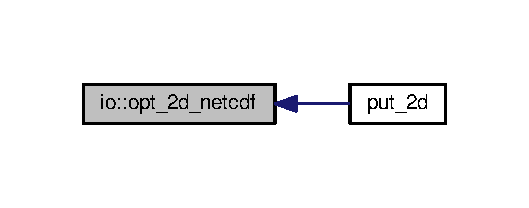
\includegraphics[width=254pt]{namespaceio_ab6bcb3dc7b4a08b242b7fbd4e11ed319_icgraph}
\end{center}
\end{figure}


\index{io@{io}!opt\+\_\+3d\+\_\+netcdf@{opt\+\_\+3d\+\_\+netcdf}}
\index{opt\+\_\+3d\+\_\+netcdf@{opt\+\_\+3d\+\_\+netcdf}!io@{io}}
\subsubsection[{\texorpdfstring{opt\+\_\+3d\+\_\+netcdf(\+O\+U\+T\+P\+U\+T\+F\+I\+L\+E, D\+U, V\+U, D\+S, P, T, S\+T\+N, W\+E\+I\+G\+H\+T, B\+O\+U\+N\+D\+A\+R\+Y, S\+T\+R\+U, S\+T\+R\+S)}{opt_3d_netcdf(OUTPUTFILE, DU, VU, DS, P, T, STN, WEIGHT, BOUNDARY, STRU, STRS)}}]{\setlength{\rightskip}{0pt plus 5cm}subroutine io\+::opt\+\_\+3d\+\_\+netcdf (
\begin{DoxyParamCaption}
\item[{character (len=$\ast$), intent(in)}]{O\+U\+T\+P\+U\+T\+F\+I\+LE, }
\item[{real (kind=rk8), dimension(\+:,\+:,\+:,\+:), intent(in)}]{DU, }
\item[{character (len=64), dimension(\+:), intent(in)}]{VU, }
\item[{real (kind=rk8), dimension(\+:,\+:,\+:), intent(in)}]{DS, }
\item[{real (kind=rk8), dimension(\+:), intent(in)}]{P, }
\item[{real (kind=rk8), dimension(\+:), intent(in)}]{T, }
\item[{character (len=64), dimension(\+:), intent(in)}]{S\+TN, }
\item[{real (kind=rk8), dimension(\+:), intent(in)}]{W\+E\+I\+G\+HT, }
\item[{integer (kind=ik4), dimension(\+:,\+:), intent(in)}]{B\+O\+U\+N\+D\+A\+RY, }
\item[{integer (kind=ik4), dimension(\+:), intent(in)}]{S\+T\+RU, }
\item[{integer (kind=ik4), dimension(\+:), intent(in)}]{S\+T\+RS}
\end{DoxyParamCaption}
)}\hypertarget{namespaceio_a63d1618c60598d1e5ac65348efb74bdc}{}\label{namespaceio_a63d1618c60598d1e5ac65348efb74bdc}


Definition at line 416 of file io.\+f90.


\begin{DoxyCode}
416     \textcolor{keywordtype}{USE }\hyperlink{namespaceportable}{portable}
417     \textcolor{keywordtype}{USE }netcdf
418 
419     \textcolor{keywordtype}{IMPLICIT NONE}
420 
421     \textcolor{keywordtype}{CHARACTER (LEN=*)}, \textcolor{keywordtype}{INTENT(IN)}                                       :: outputfile   \textcolor{comment}{! Name of the
       output file.}
422     \textcolor{keywordtype}{CHARACTER (LEN=64)}, \textcolor{keywordtype}{DIMENSION(:)}, \textcolor{keywordtype}{INTENT(IN)}                        :: vu           \textcolor{comment}{! Names of the
       variables in DU.}
423     \textcolor{keywordtype}{REAL (KIND=RK8)}, \textcolor{keywordtype}{DIMENSION(:,:,:)}, \textcolor{keywordtype}{INTENT(IN)}                       :: ds           \textcolor{comment}{! Surface level
       data.}
424     \textcolor{keywordtype}{REAL (KIND=RK8)}, \textcolor{keywordtype}{DIMENSION(:)}, \textcolor{keywordtype}{INTENT(IN)}                           :: p            \textcolor{comment}{! Pressure levels.}
425     \textcolor{keywordtype}{REAL (KIND=RK8)}, \textcolor{keywordtype}{DIMENSION(:)}, \textcolor{keywordtype}{INTENT(IN)}                           :: t            \textcolor{comment}{! Time steps.      
          }
426     \textcolor{keywordtype}{CHARACTER (LEN=64)}, \textcolor{keywordtype}{DIMENSION(:)}, \textcolor{keywordtype}{INTENT(IN)}                        :: stn          \textcolor{comment}{! Names of the
       stations.}
427     \textcolor{keywordtype}{REAL (KIND=RK8)}, \textcolor{keywordtype}{DIMENSION(:)}, \textcolor{keywordtype}{INTENT(IN)}                           :: weight       \textcolor{comment}{! Weights for each
       station.}
428     \textcolor{keywordtype}{INTEGER (KIND=IK4)}, \textcolor{keywordtype}{DIMENSION(:,:)}, \textcolor{keywordtype}{INTENT(IN)}                      :: boundary     \textcolor{comment}{! BOUNDARY array.}
429     \textcolor{keywordtype}{INTEGER (KIND=IK4)}, \textcolor{keywordtype}{DIMENSION(:)}, \textcolor{keywordtype}{INTENT(IN)}                        :: stru         \textcolor{comment}{! STRU array.}
430     \textcolor{keywordtype}{INTEGER (KIND=IK4)}, \textcolor{keywordtype}{DIMENSION(:)}, \textcolor{keywordtype}{INTENT(IN)}                        :: strs         \textcolor{comment}{! STRS array.}
431     \textcolor{comment}{!}
432     \textcolor{comment}{! Local variables.}
433     \textcolor{comment}{!}
434     \textcolor{keywordtype}{INTEGER (KIND=IK4)}          :: ncid                                                 \textcolor{comment}{! ID of NetCDF
       file.}
435     \textcolor{keywordtype}{INTEGER (KIND=IK4)}          :: v\_dim\_id, p\_dim\_id, st\_dim\_id, t\_dim\_id, str\_dim\_id, bnd\_dim\_id
436     \textcolor{keywordtype}{INTEGER (KIND=IK4)}          :: stru\_dim\_id, strs\_dim\_id, weight\_dim\_id
437     \textcolor{keywordtype}{INTEGER (KIND=IK4)}          :: v\_var\_id, p\_var\_id, st\_var\_id, t\_var\_id, du\_var\_id, ds\_var\_id, 
      boundary\_var\_id
438     \textcolor{keywordtype}{INTEGER (KIND=IK4)}          :: stru\_var\_id, strs\_var\_id, weight\_var\_id
439     \textcolor{keywordtype}{INTEGER (KIND=IK4)}          :: iost                                                 \textcolor{comment}{! I/O status.}
440     \textcolor{keywordtype}{INTEGER (KIND=IK4)}          :: ii                                                   \textcolor{comment}{! Counter.}
441     \textcolor{keywordtype}{INTEGER (KIND=IK4)}          :: strlen                                               \textcolor{comment}{! String length.}
442     \textcolor{keywordtype}{CHARACTER (LEN=64)}          :: tmpstr                                               \textcolor{comment}{! Temporary string.}
443     \textcolor{keywordtype}{REAL (KIND=RK8)}, \textcolor{keywordtype}{DIMENSION(:,:,:,:)},\textcolor{keywordtype}{INTENT(IN)}                                 :: du           \textcolor{comment}{! The 3D
       data.}
444     iost    = nf90\_noerr
445     \textcolor{comment}{!}
446     \textcolor{comment}{! Create the NetCDF file.}
447     \textcolor{comment}{!}
448     iost    = nf90\_create(outputfile, nf90\_noclobber, ncid)
449     \textcolor{keywordflow}{IF} (iost .NE. nf90\_noerr) \textcolor{keywordflow}{GO TO} 9999
450 
451     \textcolor{comment}{!}
452     \textcolor{comment}{! Define the dimensions.}
453     \textcolor{comment}{!}
454     iost    = nf90\_def\_dim(ncid, \textcolor{stringliteral}{"variables"}, \textcolor{keyword}{SIZE}(du, dim=1), v\_dim\_id)    \textcolor{comment}{! The data array contains many
       variables.}
455     \textcolor{keywordflow}{IF} (iost .NE. nf90\_noerr) \textcolor{keywordflow}{GO TO} 9999
456 
457     iost    = nf90\_def\_dim(ncid, \textcolor{stringliteral}{"levels"}, \textcolor{keyword}{SIZE}(du, dim=2), p\_dim\_id)       \textcolor{comment}{! Vertical levels.}
458     \textcolor{keywordflow}{IF} (iost .NE. nf90\_noerr) \textcolor{keywordflow}{GO TO} 9999
459 
460     iost    = nf90\_def\_dim(ncid, \textcolor{stringliteral}{"stations"}, \textcolor{keyword}{SIZE}(du, dim=3), st\_dim\_id)    \textcolor{comment}{! Stations.}
461     \textcolor{keywordflow}{IF} (iost .NE. nf90\_noerr) \textcolor{keywordflow}{GO TO} 9999
462 
463     iost    = nf90\_def\_dim(ncid, \textcolor{stringliteral}{"time"}, \textcolor{keyword}{SIZE}(du, dim=4), t\_dim\_id)         \textcolor{comment}{! Time steps.}
464     \textcolor{keywordflow}{IF} (iost .NE. nf90\_noerr) \textcolor{keywordflow}{GO TO} 9999
465 
466     iost    = nf90\_def\_dim(ncid, \textcolor{stringliteral}{"string"}, 64, str\_dim\_id)                  \textcolor{comment}{! This dimension is used for
       character strings.}
467     \textcolor{keywordflow}{IF} (iost .NE. nf90\_noerr) \textcolor{keywordflow}{GO TO} 9999
468 
469     iost    = nf90\_def\_dim(ncid, \textcolor{stringliteral}{"bnd"}, \textcolor{keyword}{SIZE}(boundary, dim=1), bnd\_dim\_id)  \textcolor{comment}{! This dimension is used for
       the BOUNDARY array.}
470     \textcolor{keywordflow}{IF} (iost .NE. nf90\_noerr) \textcolor{keywordflow}{GO TO} 9999
471 
472     iost    = nf90\_def\_dim(ncid, \textcolor{stringliteral}{"stru"}, \textcolor{keyword}{SIZE}(stru), stru\_dim\_id)           \textcolor{comment}{! This dimension is used for
       the STRU array.}
473     \textcolor{keywordflow}{IF} (iost .NE. nf90\_noerr) \textcolor{keywordflow}{GO TO} 9999
474 
475     iost    = nf90\_def\_dim(ncid, \textcolor{stringliteral}{"strs"}, \textcolor{keyword}{SIZE}(strs), strs\_dim\_id)           \textcolor{comment}{! This dimension is used for
       the STRS array.}
476     \textcolor{keywordflow}{IF} (iost .NE. nf90\_noerr) \textcolor{keywordflow}{GO TO} 9999
477 
478     iost    = nf90\_def\_dim(ncid, \textcolor{stringliteral}{"weight"}, \textcolor{keyword}{SIZE}(weight), weight\_dim\_id)     \textcolor{comment}{! This dimension is used for
       the WEIGHT array.}
479     \textcolor{keywordflow}{IF} (iost .NE. nf90\_noerr) \textcolor{keywordflow}{GO TO} 9999
480 
481     \textcolor{comment}{!}
482     \textcolor{comment}{! Define the variables.}
483     \textcolor{comment}{!}
484     iost    = nf90\_def\_var(ncid, \textcolor{stringliteral}{"variables"}, nf90\_char, (/ str\_dim\_id, v\_dim\_id /), v\_var\_id)
485     \textcolor{keywordflow}{IF} (iost .NE. nf90\_noerr) \textcolor{keywordflow}{GO TO} 9999
486 
487     iost    = nf90\_def\_var(ncid, \textcolor{stringliteral}{"levels"}, nf90\_double, (/ p\_dim\_id /), p\_var\_id)
488     \textcolor{keywordflow}{IF} (iost .NE. nf90\_noerr) \textcolor{keywordflow}{GO TO} 9999
489 
490     iost    = nf90\_def\_var(ncid, \textcolor{stringliteral}{"stations"}, nf90\_char, (/ str\_dim\_id, st\_dim\_id /), st\_var\_id)
491     \textcolor{keywordflow}{IF} (iost .NE. nf90\_noerr) \textcolor{keywordflow}{GO TO} 9999
492 
493     iost    = nf90\_def\_var(ncid, \textcolor{stringliteral}{"time"}, nf90\_double, (/ t\_dim\_id /), t\_var\_id)
494     \textcolor{keywordflow}{IF} (iost .NE. nf90\_noerr) \textcolor{keywordflow}{GO TO} 9999
495 
496     iost    = nf90\_def\_var(ncid, \textcolor{stringliteral}{"du"}, nf90\_double, (/ v\_dim\_id, p\_dim\_id, st\_dim\_id, t\_dim\_id /), 
      du\_var\_id)
497     \textcolor{keywordflow}{IF} (iost .NE. nf90\_noerr) \textcolor{keywordflow}{GO TO} 9999
498 
499     iost    = nf90\_def\_var(ncid, \textcolor{stringliteral}{"ds"}, nf90\_double, (/ v\_dim\_id, st\_dim\_id, t\_dim\_id /), ds\_var\_id)
500     \textcolor{keywordflow}{IF} (iost .NE. nf90\_noerr) \textcolor{keywordflow}{GO TO} 9999
501 
502     iost    = nf90\_def\_var(ncid, \textcolor{stringliteral}{"boundary"}, nf90\_int, (/ bnd\_dim\_id, t\_dim\_id /), boundary\_var\_id)
503     \textcolor{keywordflow}{IF} (iost .NE. nf90\_noerr) \textcolor{keywordflow}{GO TO} 9999
504 
505     iost    = nf90\_def\_var(ncid, \textcolor{stringliteral}{"stru"}, nf90\_int, (/ stru\_dim\_id /), stru\_var\_id)
506     \textcolor{keywordflow}{IF} (iost .NE. nf90\_noerr) \textcolor{keywordflow}{GO TO} 9999
507 
508     iost    = nf90\_def\_var(ncid, \textcolor{stringliteral}{"strs"}, nf90\_int, (/ strs\_dim\_id /), strs\_var\_id)
509     \textcolor{keywordflow}{IF} (iost .NE. nf90\_noerr) \textcolor{keywordflow}{GO TO} 9999
510 
511     iost    = nf90\_def\_var(ncid, \textcolor{stringliteral}{"weight"}, nf90\_double, (/ weight\_dim\_id /), weight\_var\_id)
512     \textcolor{keywordflow}{IF} (iost .NE. nf90\_noerr) \textcolor{keywordflow}{GO TO} 9999
513 
514     \textcolor{comment}{!}
515     \textcolor{comment}{! Create various attributes. Make sure strings are null terminated (for C programs).}
516     \textcolor{comment}{!}
517 \textcolor{comment}{!    IOST    = NF90\_PUT\_ATT(NCID, NF90\_GLOBAL, "instrument", TRIM(INSTRUMENT)//CHAR(0))}
518 \textcolor{comment}{!    IF (IOST .NE. NF90\_NOERR) GO TO 9999}
519     iost    = nf90\_put\_att(ncid, t\_var\_id, \textcolor{stringliteral}{"units"}, \textcolor{stringliteral}{'Days since 2004-10-01T00:00:00 UTC'}//char(0))
520     \textcolor{keywordflow}{IF} (iost .NE. nf90\_noerr) \textcolor{keywordflow}{GO TO} 9999
521     iost    = nf90\_put\_att(ncid, p\_var\_id, \textcolor{stringliteral}{"units"}, \textcolor{stringliteral}{'hPa'}//char(0))
522     \textcolor{keywordflow}{IF} (iost .NE. nf90\_noerr) \textcolor{keywordflow}{GO TO} 9999
523 
524     \textcolor{comment}{!}
525     \textcolor{comment}{! We've finished defining stuff, leave the definition mode.}
526     \textcolor{comment}{!}
527     iost    = nf90\_enddef(ncid)
528     \textcolor{keywordflow}{IF} (iost .NE. nf90\_noerr) \textcolor{keywordflow}{GO TO} 9999
529 
530     \textcolor{comment}{!}
531     \textcolor{comment}{! Write the names of the variables. Terminate strings with a null byte, in case the data are
       subsequently read by a C program.}
532     \textcolor{comment}{!}
533     \textcolor{keywordflow}{IF} (\textcolor{keyword}{SIZE}(du, dim=1) .NE. \textcolor{keyword}{SIZE}(vu)) \textcolor{keywordflow}{THEN}
534         print *,\textcolor{stringliteral}{'E: Size of variable dimension in DU is different than VU'}
535         stop \textcolor{stringliteral}{'1'}
536 \textcolor{keywordflow}{    END IF}
537 
538     \textcolor{keywordflow}{DO} ii=1,\textcolor{keyword}{SIZE}(du, dim=1)
539         tmpstr      = trim(vu(ii))
540         strlen      = min(63, len\_trim(tmpstr))           \textcolor{comment}{! The characters after this positon will be
       replaced by null characters.}
541         tmpstr(strlen+1:64)    = repeat(char(0), 64-strlen)
542         iost        = nf90\_put\_var(ncid, v\_var\_id, tmpstr, (/ 1, ii /), (/ 64, 1 /))
543         \textcolor{keywordflow}{IF} (iost .NE. nf90\_noerr) \textcolor{keywordflow}{GO TO} 9999
544 \textcolor{keywordflow}{    END DO}
545 
546     \textcolor{comment}{!}
547     \textcolor{comment}{! Write the names of the stations. Terminate strings with a null byte, in case the data are
       subsequently read by a C program.}
548     \textcolor{comment}{!}
549     \textcolor{keywordflow}{DO} ii=1,\textcolor{keyword}{SIZE}(du, dim=3)
550         tmpstr  = trim(stn(ii))
551         strlen  = min(63, len\_trim(tmpstr))           \textcolor{comment}{! The characters after this positon will be replaced
       by null characters.}
552         tmpstr(strlen+1:64)    = repeat(char(0), 64-strlen)
553         iost    = nf90\_put\_var(ncid, st\_var\_id, tmpstr, (/ 1, ii /), (/ 64, 1 /))
554         \textcolor{keywordflow}{IF} (iost .NE. nf90\_noerr) \textcolor{keywordflow}{GO TO} 9999
555 \textcolor{keywordflow}{    END DO}
556 
557     \textcolor{comment}{!}
558     \textcolor{comment}{! Write the pressure levels.}
559     \textcolor{comment}{!}
560     iost    = nf90\_put\_var(ncid, p\_var\_id, p)
561     \textcolor{keywordflow}{IF} (iost .NE. nf90\_noerr) \textcolor{keywordflow}{GO TO} 9999
562 
563     \textcolor{comment}{!}
564     \textcolor{comment}{! Write the time steps.}
565     \textcolor{comment}{!}
566     iost    = nf90\_put\_var(ncid, t\_var\_id, t)
567     \textcolor{keywordflow}{IF} (iost .NE. nf90\_noerr) \textcolor{keywordflow}{GO TO} 9999
568 
569     \textcolor{comment}{!}
570     \textcolor{comment}{! Write the data arrays.}
571     \textcolor{comment}{!}
572     iost    = nf90\_put\_var(ncid, du\_var\_id, du)
573     \textcolor{keywordflow}{IF} (iost .NE. nf90\_noerr) \textcolor{keywordflow}{GO TO} 9999
574 
575     iost    = nf90\_put\_var(ncid, ds\_var\_id, ds)
576     \textcolor{keywordflow}{IF} (iost .NE. nf90\_noerr) \textcolor{keywordflow}{GO TO} 9999
577 
578     iost    = nf90\_put\_var(ncid, boundary\_var\_id, boundary)
579     \textcolor{keywordflow}{IF} (iost .NE. nf90\_noerr) \textcolor{keywordflow}{GO TO} 9999
580 
581     iost    = nf90\_put\_var(ncid, stru\_var\_id, stru)
582     \textcolor{keywordflow}{IF} (iost .NE. nf90\_noerr) \textcolor{keywordflow}{GO TO} 9999
583 
584     iost    = nf90\_put\_var(ncid, strs\_var\_id, strs)
585     \textcolor{keywordflow}{IF} (iost .NE. nf90\_noerr) \textcolor{keywordflow}{GO TO} 9999
586 
587     iost    = nf90\_put\_var(ncid, weight\_var\_id, weight)
588     \textcolor{keywordflow}{IF} (iost .NE. nf90\_noerr) \textcolor{keywordflow}{GO TO} 9999
589 
590     \textcolor{comment}{!}
591     \textcolor{comment}{! Close the NetCDF file.}
592     \textcolor{comment}{!}
593     iost    = nf90\_close(ncid)
594     \textcolor{keywordflow}{IF} (iost .NE. nf90\_noerr) \textcolor{keywordflow}{GO TO} 9999
595 
596     \textcolor{comment}{!}
597     \textcolor{comment}{! Catch any NetCDF errors here.}
598     \textcolor{comment}{!}
599     9999 \textcolor{keywordflow}{CONTINUE}
600     \textcolor{keywordflow}{IF} (iost .NE. nf90\_noerr) \textcolor{keywordflow}{THEN}
601         print *,\textcolor{stringliteral}{'E: Problem creating NetCDF file '},outputfile
602         print *, trim(nf90\_strerror(iost))
603         stop \textcolor{stringliteral}{'1'}
604 \textcolor{keywordflow}{    END IF}
605 
\end{DoxyCode}


Here is the caller graph for this function\+:\nopagebreak
\begin{figure}[H]
\begin{center}
\leavevmode
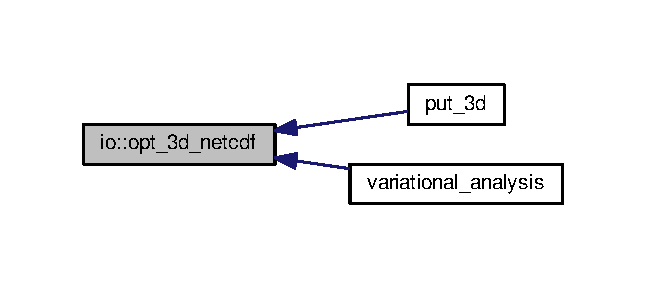
\includegraphics[width=310pt]{namespaceio_a63d1618c60598d1e5ac65348efb74bdc_icgraph}
\end{center}
\end{figure}


\index{io@{io}!opt\+\_\+budget\+\_\+netcdf@{opt\+\_\+budget\+\_\+netcdf}}
\index{opt\+\_\+budget\+\_\+netcdf@{opt\+\_\+budget\+\_\+netcdf}!io@{io}}
\subsubsection[{\texorpdfstring{opt\+\_\+budget\+\_\+netcdf(\+O\+U\+T\+P\+U\+T\+F\+I\+L\+E, B\+U\+D\+G\+E\+T\+\_\+\+C\+O\+L\+U\+M\+N, B\+U\+D\+G\+E\+T\+\_\+\+L\+A\+Y\+E\+R, V\+B\+U\+D\+G\+E\+T\+\_\+\+C\+O\+L\+U\+M\+N, V\+B\+U\+D\+G\+E\+T\+\_\+\+L\+A\+Y\+E\+R, A\+V\+E\+\_\+\+Q\+S, A\+V\+E\+\_\+\+S\+S, P, T)}{opt_budget_netcdf(OUTPUTFILE, BUDGET_COLUMN, BUDGET_LAYER, VBUDGET_COLUMN, VBUDGET_LAYER, AVE_QS, AVE_SS, P, T)}}]{\setlength{\rightskip}{0pt plus 5cm}subroutine io\+::opt\+\_\+budget\+\_\+netcdf (
\begin{DoxyParamCaption}
\item[{character (len=$\ast$), intent(in)}]{O\+U\+T\+P\+U\+T\+F\+I\+LE, }
\item[{real (kind=rk8), dimension(\+:,\+:,\+:), intent(in)}]{B\+U\+D\+G\+E\+T\+\_\+\+C\+O\+L\+U\+MN, }
\item[{real (kind=rk8), dimension(\+:,\+:,\+:,\+:), intent(in)}]{B\+U\+D\+G\+E\+T\+\_\+\+L\+A\+Y\+ER, }
\item[{character (len=64), dimension(\+:,\+:), intent(in)}]{V\+B\+U\+D\+G\+E\+T\+\_\+\+C\+O\+L\+U\+MN, }
\item[{character (len=64), dimension(\+:,\+:), intent(in)}]{V\+B\+U\+D\+G\+E\+T\+\_\+\+L\+A\+Y\+ER, }
\item[{real (kind=rk8), dimension(\+:), intent(in)}]{A\+V\+E\+\_\+\+QS, }
\item[{real (kind=rk8), dimension(\+:), intent(in)}]{A\+V\+E\+\_\+\+SS, }
\item[{real (kind=rk8), dimension(\+:), intent(in)}]{P, }
\item[{real (kind=rk8), dimension(\+:), intent(in)}]{T}
\end{DoxyParamCaption}
)}\hypertarget{namespaceio_ab1a423779bddf2d4557f39dd81431d93}{}\label{namespaceio_ab1a423779bddf2d4557f39dd81431d93}


Definition at line 893 of file io.\+f90.


\begin{DoxyCode}
893     \textcolor{keywordtype}{USE }\hyperlink{namespaceportable}{portable}
894     \textcolor{keywordtype}{USE }netcdf
895 
896     \textcolor{keywordtype}{IMPLICIT NONE}
897 
898     \textcolor{keywordtype}{CHARACTER (LEN=*)}, \textcolor{keywordtype}{INTENT(IN)}                                       :: outputfile       \textcolor{comment}{! Name of the
       output file.}
899     \textcolor{keywordtype}{REAL (KIND=RK8)}, \textcolor{keywordtype}{DIMENSION(:,:,:)}, \textcolor{keywordtype}{INTENT(IN)}                       :: budget\_column
900     \textcolor{keywordtype}{REAL (KIND=RK8)}, \textcolor{keywordtype}{DIMENSION(:,:,:,:)}, \textcolor{keywordtype}{INTENT(IN)}                     :: budget\_layer
901     \textcolor{keywordtype}{CHARACTER (LEN=64)}, \textcolor{keywordtype}{DIMENSION(:,:)}, \textcolor{keywordtype}{INTENT(IN)}                      :: vbudget\_column
902     \textcolor{keywordtype}{CHARACTER (LEN=64)}, \textcolor{keywordtype}{DIMENSION(:,:)}, \textcolor{keywordtype}{INTENT(IN)}                      :: vbudget\_layer
903     \textcolor{keywordtype}{REAL (KIND=RK8)}, \textcolor{keywordtype}{DIMENSION(:)}, \textcolor{keywordtype}{INTENT(IN)}                           :: ave\_qs
904     \textcolor{keywordtype}{REAL (KIND=RK8)}, \textcolor{keywordtype}{DIMENSION(:)}, \textcolor{keywordtype}{INTENT(IN)}                           :: ave\_ss
905     \textcolor{keywordtype}{REAL (KIND=RK8)}, \textcolor{keywordtype}{DIMENSION(:)}, \textcolor{keywordtype}{INTENT(IN)}                           :: p
906     \textcolor{keywordtype}{REAL (KIND=RK8)}, \textcolor{keywordtype}{DIMENSION(:)}, \textcolor{keywordtype}{INTENT(IN)}                           :: t
907 
908     \textcolor{comment}{!}
909     \textcolor{comment}{! Local variables.}
910     \textcolor{comment}{!}
911     \textcolor{keywordtype}{INTEGER (KIND=IK4)}          :: ncid                                                 \textcolor{comment}{! ID of NetCDF
       file.}
912     \textcolor{keywordtype}{INTEGER (KIND=IK4)}          :: bcv\_dim\_id, bct\_dim\_id, blv\_dim\_id, blt\_dim\_id, p\_dim\_id, t\_dim\_id, 
      str\_dim\_id
913     \textcolor{keywordtype}{INTEGER (KIND=IK4)}          :: bc\_var\_id, bl\_var\_id, vbc\_var\_id, vbl\_var\_id, ave\_qs\_var\_id, 
      ave\_ss\_var\_id, p\_var\_id, t\_var\_id
914     \textcolor{keywordtype}{INTEGER (KIND=IK4)}          :: iost                                                 \textcolor{comment}{! I/O status.}
915     \textcolor{keywordtype}{INTEGER (KIND=IK4)}          :: ii, jj                                               \textcolor{comment}{! Counter.}
916     \textcolor{keywordtype}{INTEGER (KIND=IK4)}          :: strlen                                               \textcolor{comment}{! String length.}
917     \textcolor{keywordtype}{CHARACTER (LEN=64)}          :: tmpstr                                               \textcolor{comment}{! Temporary string.}
918 
919     \textcolor{comment}{!}
920     \textcolor{comment}{! Create the NetCDF file.}
921     \textcolor{comment}{!}
922     iost    = nf90\_noerr
923     iost    = nf90\_create(outputfile, nf90\_noclobber, ncid)
924     \textcolor{keywordflow}{IF} (iost .NE. nf90\_noerr) \textcolor{keywordflow}{GO TO} 9999
925 
926     \textcolor{comment}{!}
927     \textcolor{comment}{! Define the dimensions.}
928     \textcolor{comment}{!}
929     iost    = nf90\_def\_dim(ncid, \textcolor{stringliteral}{"bcv"}, \textcolor{keyword}{SIZE}(budget\_column, dim=1), bcv\_dim\_id)
930     \textcolor{keywordflow}{IF} (iost .NE. nf90\_noerr) \textcolor{keywordflow}{GO TO} 9999
931 
932     iost    = nf90\_def\_dim(ncid, \textcolor{stringliteral}{"bct"}, \textcolor{keyword}{SIZE}(budget\_column, dim=2), bct\_dim\_id)
933     \textcolor{keywordflow}{IF} (iost .NE. nf90\_noerr) \textcolor{keywordflow}{GO TO} 9999
934 
935     iost    = nf90\_def\_dim(ncid, \textcolor{stringliteral}{"blv"}, \textcolor{keyword}{SIZE}(budget\_layer, dim=1), blv\_dim\_id)
936     \textcolor{keywordflow}{IF} (iost .NE. nf90\_noerr) \textcolor{keywordflow}{GO TO} 9999
937 
938     iost    = nf90\_def\_dim(ncid, \textcolor{stringliteral}{"blt"}, \textcolor{keyword}{SIZE}(budget\_layer, dim=2), blt\_dim\_id)
939     \textcolor{keywordflow}{IF} (iost .NE. nf90\_noerr) \textcolor{keywordflow}{GO TO} 9999
940 
941     iost    = nf90\_def\_dim(ncid, \textcolor{stringliteral}{"levels"}, \textcolor{keyword}{SIZE}(p, dim=1), p\_dim\_id)
942     \textcolor{keywordflow}{IF} (iost .NE. nf90\_noerr) \textcolor{keywordflow}{GO TO} 9999
943 
944     iost    = nf90\_def\_dim(ncid, \textcolor{stringliteral}{"time"}, \textcolor{keyword}{SIZE}(t, dim=1), t\_dim\_id)
945     \textcolor{keywordflow}{IF} (iost .NE. nf90\_noerr) \textcolor{keywordflow}{GO TO} 9999
946 
947     iost    = nf90\_def\_dim(ncid, \textcolor{stringliteral}{"string"}, 64, str\_dim\_id)                  \textcolor{comment}{! This dimension is used for
       character strings.}
948     \textcolor{keywordflow}{IF} (iost .NE. nf90\_noerr) \textcolor{keywordflow}{GO TO} 9999
949 
950     \textcolor{comment}{!}
951     \textcolor{comment}{! Define the variables.}
952     \textcolor{comment}{!}
953     iost    = nf90\_def\_var(ncid, \textcolor{stringliteral}{"budget\_column"}, nf90\_double, (/ bcv\_dim\_id, bct\_dim\_id, t\_dim\_id /), 
      bc\_var\_id)
954     \textcolor{keywordflow}{IF} (iost .NE. nf90\_noerr) \textcolor{keywordflow}{GO TO} 9999
955 
956     iost    = nf90\_def\_var(ncid, \textcolor{stringliteral}{"budget\_layer"}, nf90\_double, (/ blv\_dim\_id, blt\_dim\_id, p\_dim\_id, t\_dim\_id
       /), bl\_var\_id)
957     \textcolor{keywordflow}{IF} (iost .NE. nf90\_noerr) \textcolor{keywordflow}{GO TO} 9999
958 
959     iost    = nf90\_def\_var(ncid, \textcolor{stringliteral}{"vbudget\_column"}, nf90\_char, (/ str\_dim\_id, bcv\_dim\_id, bct\_dim\_id /), 
      vbc\_var\_id)
960     \textcolor{keywordflow}{IF} (iost .NE. nf90\_noerr) \textcolor{keywordflow}{GO TO} 9999
961 
962     iost    = nf90\_def\_var(ncid, \textcolor{stringliteral}{"vbudget\_layer"}, nf90\_char, (/ str\_dim\_id, blv\_dim\_id, blt\_dim\_id /), 
      vbl\_var\_id)
963     \textcolor{keywordflow}{IF} (iost .NE. nf90\_noerr) \textcolor{keywordflow}{GO TO} 9999
964 
965     iost    = nf90\_def\_var(ncid, \textcolor{stringliteral}{"ave\_qs"}, nf90\_double, (/ t\_dim\_id /), ave\_qs\_var\_id)
966     \textcolor{keywordflow}{IF} (iost .NE. nf90\_noerr) \textcolor{keywordflow}{GO TO} 9999
967 
968     iost    = nf90\_def\_var(ncid, \textcolor{stringliteral}{"ave\_ss"}, nf90\_double, (/ t\_dim\_id /), ave\_ss\_var\_id)
969     \textcolor{keywordflow}{IF} (iost .NE. nf90\_noerr) \textcolor{keywordflow}{GO TO} 9999
970 
971     iost    = nf90\_def\_var(ncid, \textcolor{stringliteral}{"levels"}, nf90\_double, (/ p\_dim\_id /), p\_var\_id)
972     \textcolor{keywordflow}{IF} (iost .NE. nf90\_noerr) \textcolor{keywordflow}{GO TO} 9999
973 
974     iost    = nf90\_def\_var(ncid, \textcolor{stringliteral}{"time"}, nf90\_double, (/ t\_dim\_id /), t\_var\_id)
975     \textcolor{keywordflow}{IF} (iost .NE. nf90\_noerr) \textcolor{keywordflow}{GO TO} 9999
976 
977     \textcolor{comment}{!}
978     \textcolor{comment}{! Create various attributes. Make sure strings are null terminated (for C programs).}
979     \textcolor{comment}{!}
980     iost    = nf90\_put\_att(ncid, t\_var\_id, \textcolor{stringliteral}{"units"}, \textcolor{stringliteral}{'Days since 2004-10-01T00:00:00 UTC'}//char(0))
981     \textcolor{keywordflow}{IF} (iost .NE. nf90\_noerr) \textcolor{keywordflow}{GO TO} 9999
982     iost    = nf90\_put\_att(ncid, p\_var\_id, \textcolor{stringliteral}{"units"}, \textcolor{stringliteral}{'hPa'}//char(0))
983     \textcolor{keywordflow}{IF} (iost .NE. nf90\_noerr) \textcolor{keywordflow}{GO TO} 9999
984 
985     \textcolor{comment}{!}
986     \textcolor{comment}{! We've finished defining stuff, leave the definition mode.}
987     \textcolor{comment}{!}
988     iost    = nf90\_enddef(ncid)
989     \textcolor{keywordflow}{IF} (iost .NE. nf90\_noerr) \textcolor{keywordflow}{GO TO} 9999
990 
991     \textcolor{comment}{!}
992     \textcolor{comment}{! Write VBUDGET\_COLUMN and VBUDGET\_LAYER. Terminate strings with a null byte, in case the data are
       subsequently }
993     \textcolor{comment}{! read by a C program.}
994     \textcolor{comment}{!}
995     \textcolor{keywordflow}{DO} ii=1,\textcolor{keyword}{SIZE}(budget\_column, dim=1)
996         \textcolor{keywordflow}{DO} jj=1,\textcolor{keyword}{SIZE}(budget\_column, dim=2)
997             tmpstr      = trim(vbudget\_column(ii,jj))
998             strlen      = min(63, len\_trim(tmpstr))         \textcolor{comment}{! The characters after this positon will be
       replaced by null characters.}
999             tmpstr(strlen+1:64)    = repeat(char(0), 64-strlen)
1000             iost        = nf90\_put\_var(ncid, vbc\_var\_id, tmpstr, (/ 1, ii, jj /), (/ 64, 1, 1 /))
1001             \textcolor{keywordflow}{IF} (iost .NE. nf90\_noerr) \textcolor{keywordflow}{GO TO} 9999
1002 \textcolor{keywordflow}{        END DO}
1003 \textcolor{keywordflow}{    END DO}
1004 
1005     \textcolor{keywordflow}{DO} ii=1,\textcolor{keyword}{SIZE}(budget\_layer, dim=1)
1006         \textcolor{keywordflow}{DO} jj=1,\textcolor{keyword}{SIZE}(budget\_layer, dim=2)
1007             tmpstr      = trim(vbudget\_layer(ii,jj))
1008             strlen      = min(63, len\_trim(tmpstr))         \textcolor{comment}{! The characters after this positon will be
       replaced by null characters.}
1009             tmpstr(strlen+1:64)    = repeat(char(0), 64-strlen)
1010             iost        = nf90\_put\_var(ncid, vbl\_var\_id, tmpstr, (/ 1, ii, jj /), (/ 64, 1, 1 /))
1011             \textcolor{keywordflow}{IF} (iost .NE. nf90\_noerr) \textcolor{keywordflow}{GO TO} 9999
1012 \textcolor{keywordflow}{        END DO}
1013 \textcolor{keywordflow}{    END DO}
1014 
1015     \textcolor{comment}{!}
1016     \textcolor{comment}{! Write the pressure levels.}
1017     \textcolor{comment}{!}
1018     iost    = nf90\_put\_var(ncid, p\_var\_id, p)
1019     \textcolor{keywordflow}{IF} (iost .NE. nf90\_noerr) \textcolor{keywordflow}{GO TO} 9999
1020 
1021     \textcolor{comment}{!}
1022     \textcolor{comment}{! Write the time steps.}
1023     \textcolor{comment}{!}
1024     iost    = nf90\_put\_var(ncid, t\_var\_id, t)
1025     \textcolor{keywordflow}{IF} (iost .NE. nf90\_noerr) \textcolor{keywordflow}{GO TO} 9999
1026 
1027     \textcolor{comment}{!}
1028     \textcolor{comment}{! Write the data arrays.}
1029     \textcolor{comment}{!}
1030     iost    = nf90\_put\_var(ncid, bc\_var\_id, budget\_column)
1031     \textcolor{keywordflow}{IF} (iost .NE. nf90\_noerr) \textcolor{keywordflow}{GO TO} 9999
1032 
1033     iost    = nf90\_put\_var(ncid, bl\_var\_id, budget\_layer)
1034     \textcolor{keywordflow}{IF} (iost .NE. nf90\_noerr) \textcolor{keywordflow}{GO TO} 9999
1035 
1036     iost    = nf90\_put\_var(ncid, ave\_qs\_var\_id, ave\_qs)
1037     \textcolor{keywordflow}{IF} (iost .NE. nf90\_noerr) \textcolor{keywordflow}{GO TO} 9999
1038 
1039     iost    = nf90\_put\_var(ncid, ave\_ss\_var\_id, ave\_ss)
1040     \textcolor{keywordflow}{IF} (iost .NE. nf90\_noerr) \textcolor{keywordflow}{GO TO} 9999
1041 
1042     \textcolor{comment}{!}
1043     \textcolor{comment}{! Close the NetCDF file.}
1044     \textcolor{comment}{!}
1045     iost    = nf90\_close(ncid)
1046     \textcolor{keywordflow}{IF} (iost .NE. nf90\_noerr) \textcolor{keywordflow}{GO TO} 9999
1047 
1048     \textcolor{comment}{!}
1049     \textcolor{comment}{! Catch any NetCDF errors here.}
1050     \textcolor{comment}{!}
1051     9999 \textcolor{keywordflow}{CONTINUE}
1052     \textcolor{keywordflow}{IF} (iost .NE. nf90\_noerr) \textcolor{keywordflow}{THEN}
1053         print *,\textcolor{stringliteral}{'E: Problem creating NetCDF file '},outputfile
1054         print *, trim(nf90\_strerror(iost))
1055         stop \textcolor{stringliteral}{'1'}
1056 \textcolor{keywordflow}{    END IF}
1057 
\end{DoxyCode}


Here is the caller graph for this function\+:\nopagebreak
\begin{figure}[H]
\begin{center}
\leavevmode
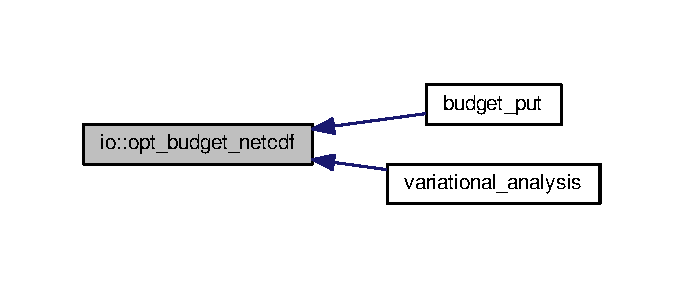
\includegraphics[width=328pt]{namespaceio_ab1a423779bddf2d4557f39dd81431d93_icgraph}
\end{center}
\end{figure}


\index{io@{io}!opt\+\_\+forcing\+\_\+netcdf@{opt\+\_\+forcing\+\_\+netcdf}}
\index{opt\+\_\+forcing\+\_\+netcdf@{opt\+\_\+forcing\+\_\+netcdf}!io@{io}}
\subsubsection[{\texorpdfstring{opt\+\_\+forcing\+\_\+netcdf(\+O\+U\+T\+P\+U\+T\+F\+I\+L\+E, S\+F\+C\+\_\+\+D\+A\+T\+A, M\+L\+\_\+\+D\+A\+T\+A, C\+F\+\_\+\+L\+O\+N, C\+F\+\_\+\+L\+A\+T, C\+F\+\_\+\+P\+H\+I\+S, P\+L\+E\+V\+S)}{opt_forcing_netcdf(OUTPUTFILE, SFC_DATA, ML_DATA, CF_LON, CF_LAT, CF_PHIS, PLEVS)}}]{\setlength{\rightskip}{0pt plus 5cm}subroutine io\+::opt\+\_\+forcing\+\_\+netcdf (
\begin{DoxyParamCaption}
\item[{character (len=$\ast$), intent(in)}]{O\+U\+T\+P\+U\+T\+F\+I\+LE, }
\item[{real (kind=rk8), dimension(\+:,\+:), intent(in)}]{S\+F\+C\+\_\+\+D\+A\+TA, }
\item[{real (kind=rk8), dimension(\+:,\+:,\+:), intent(in)}]{M\+L\+\_\+\+D\+A\+TA, }
\item[{real (kind=rk4), intent(in)}]{C\+F\+\_\+\+L\+ON, }
\item[{real (kind=rk4), intent(in)}]{C\+F\+\_\+\+L\+AT, }
\item[{real (kind=rk4), intent(in)}]{C\+F\+\_\+\+P\+H\+IS, }
\item[{real (kind=rk8), dimension(\+:), intent(in)}]{P\+L\+E\+VS}
\end{DoxyParamCaption}
)}\hypertarget{namespaceio_a50ab1073758d8d341087a0755354011d}{}\label{namespaceio_a50ab1073758d8d341087a0755354011d}


Definition at line 1708 of file io.\+f90.


\begin{DoxyCode}
1708     \textcolor{keywordtype}{USE }\hyperlink{namespaceportable}{portable}
1709     \textcolor{keywordtype}{USE }netcdf
1710     \textcolor{keywordtype}{USE }\hyperlink{namespacetime}{time}
1711 
1712     \textcolor{keywordtype}{IMPLICIT NONE}
1713 
1714     \textcolor{keywordtype}{CHARACTER (LEN=*)}, \textcolor{keywordtype}{INTENT(IN)}                                       :: outputfile       \textcolor{comment}{! Name of the
       output file.}
1715     \textcolor{keywordtype}{REAL (KIND=RK8)}, \textcolor{keywordtype}{DIMENSION(:,:)}, \textcolor{keywordtype}{INTENT(IN)}                         :: sfc\_data         \textcolor{comment}{! Surface
       forcing data.}
1716     \textcolor{keywordtype}{REAL (KIND=RK8)}, \textcolor{keywordtype}{DIMENSION(:,:,:)}, \textcolor{keywordtype}{INTENT(IN)}                       :: ml\_data          \textcolor{comment}{! Multi-levcel
       forcing data.}
1717     \textcolor{keywordtype}{REAL (KIND=RK4)}, \textcolor{keywordtype}{INTENT(IN)}                                         :: cf\_lon           \textcolor{comment}{! Central
       facility longitude.}
1718     \textcolor{keywordtype}{REAL (KIND=RK4)}, \textcolor{keywordtype}{INTENT(IN)}                                         :: cf\_lat           \textcolor{comment}{! Central
       facility latitude.}
1719     \textcolor{keywordtype}{REAL (KIND=RK4)}, \textcolor{keywordtype}{INTENT(IN)}                                         :: cf\_phis          \textcolor{comment}{! Central
       facility geopotential height.}
1720     \textcolor{keywordtype}{REAL (KIND=RK8)}, \textcolor{keywordtype}{DIMENSION(:)}, \textcolor{keywordtype}{INTENT(IN)}                           :: plevs            \textcolor{comment}{! Pressure
       levels in analysis.}
1721 
1722     \textcolor{comment}{!}
1723     \textcolor{comment}{! Local variables.}
1724     \textcolor{comment}{!}
1725     \textcolor{keywordtype}{INTEGER (KIND=IK4)}                  :: ncid                                                 \textcolor{comment}{! ID of
       NetCDF file.}
1726     \textcolor{keywordtype}{INTEGER (KIND=IK4)}                  :: time\_dim\_id, lev\_dim\_id                              \textcolor{comment}{! Dimension
       IDs.}
1727     \textcolor{keywordtype}{INTEGER (KIND=IK4)}                  :: base\_time\_var\_id                                     \textcolor{comment}{! Variable
       ID for base\_time}
1728     \textcolor{keywordtype}{INTEGER (KIND=IK4)}                  :: time\_var\_id
1729     \textcolor{keywordtype}{INTEGER (KIND=IK4)}                  :: time\_offset\_var\_id
1730     \textcolor{keywordtype}{INTEGER (KIND=IK4)}                  :: year\_var\_id
1731     \textcolor{keywordtype}{INTEGER (KIND=IK4)}                  :: month\_var\_id
1732     \textcolor{keywordtype}{INTEGER (KIND=IK4)}                  :: day\_var\_id
1733     \textcolor{keywordtype}{INTEGER (KIND=IK4)}                  :: hour\_var\_id
1734     \textcolor{keywordtype}{INTEGER (KIND=IK4)}                  :: minute\_var\_id
1735     \textcolor{keywordtype}{INTEGER (KIND=IK4)}                  :: lat\_var\_id
1736     \textcolor{keywordtype}{INTEGER (KIND=IK4)}                  :: lon\_var\_id
1737     \textcolor{keywordtype}{INTEGER (KIND=IK4)}                  :: phis\_var\_id
1738     \textcolor{keywordtype}{INTEGER (KIND=IK4)}                  :: lev\_var\_id
1739     \textcolor{keywordtype}{INTEGER (KIND=IK4)}                  :: temp\_var\_id
1740     \textcolor{keywordtype}{INTEGER (KIND=IK4)}                  :: q\_var\_id
1741     \textcolor{keywordtype}{INTEGER (KIND=IK4)}                  :: u\_var\_id
1742     \textcolor{keywordtype}{INTEGER (KIND=IK4)}                  :: v\_var\_id
1743     \textcolor{keywordtype}{INTEGER (KIND=IK4)}                  :: omega\_var\_id
1744     \textcolor{keywordtype}{INTEGER (KIND=IK4)}                  :: div\_var\_id
1745     \textcolor{keywordtype}{INTEGER (KIND=IK4)}                  :: tadvh\_var\_id
1746     \textcolor{keywordtype}{INTEGER (KIND=IK4)}                  :: tadvv\_var\_id
1747     \textcolor{keywordtype}{INTEGER (KIND=IK4)}                  :: qadvh\_var\_id
1748     \textcolor{keywordtype}{INTEGER (KIND=IK4)}                  :: qadvv\_var\_id
1749     \textcolor{keywordtype}{INTEGER (KIND=IK4)}                  :: s\_var\_id
1750     \textcolor{keywordtype}{INTEGER (KIND=IK4)}                  :: sadvh\_var\_id
1751     \textcolor{keywordtype}{INTEGER (KIND=IK4)}                  :: sadvv\_var\_id
1752     \textcolor{keywordtype}{INTEGER (KIND=IK4)}                  :: dsdt\_var\_id
1753     \textcolor{keywordtype}{INTEGER (KIND=IK4)}                  :: dtdt\_var\_id
1754     \textcolor{keywordtype}{INTEGER (KIND=IK4)}                  :: dqdt\_var\_id
1755     \textcolor{keywordtype}{INTEGER (KIND=IK4)}                  :: q1\_var\_id
1756     \textcolor{keywordtype}{INTEGER (KIND=IK4)}                  :: q2\_var\_id
1757     \textcolor{keywordtype}{INTEGER (KIND=IK4)}                  :: cld\_var\_id
1758     \textcolor{keywordtype}{INTEGER (KIND=IK4)}                  :: prec\_var\_id
1759     \textcolor{keywordtype}{INTEGER (KIND=IK4)}                  :: lh\_var\_id
1760     \textcolor{keywordtype}{INTEGER (KIND=IK4)}                  :: sh\_var\_id
1761     \textcolor{keywordtype}{INTEGER (KIND=IK4)}                  :: psa\_var\_id
1762     \textcolor{keywordtype}{INTEGER (KIND=IK4)}                  :: psi\_var\_id
1763     \textcolor{keywordtype}{INTEGER (KIND=IK4)}                  :: tsair\_var\_id
1764     \textcolor{keywordtype}{INTEGER (KIND=IK4)}                  :: tskin\_var\_id
1765     \textcolor{keywordtype}{INTEGER (KIND=IK4)}                  :: rhair\_var\_id
1766     \textcolor{keywordtype}{INTEGER (KIND=IK4)}                  :: wspd\_var\_id
1767     \textcolor{keywordtype}{INTEGER (KIND=IK4)}                  :: us\_var\_id
1768     \textcolor{keywordtype}{INTEGER (KIND=IK4)}                  :: vs\_var\_id
1769     \textcolor{keywordtype}{INTEGER (KIND=IK4)}                  :: srfrad\_var\_id
1770     \textcolor{keywordtype}{INTEGER (KIND=IK4)}                  :: flut\_var\_id
1771     \textcolor{keywordtype}{INTEGER (KIND=IK4)}                  :: fsnt\_var\_id
1772     \textcolor{keywordtype}{INTEGER (KIND=IK4)}                  :: solin\_var\_id
1773     \textcolor{keywordtype}{INTEGER (KIND=IK4)}                  :: cldlow\_var\_id
1774     \textcolor{keywordtype}{INTEGER (KIND=IK4)}                  :: cldmed\_var\_id
1775     \textcolor{keywordtype}{INTEGER (KIND=IK4)}                  :: cldhgh\_var\_id
1776     \textcolor{keywordtype}{INTEGER (KIND=IK4)}                  :: cldtot\_var\_id
1777     \textcolor{keywordtype}{INTEGER (KIND=IK4)}                  :: cldthk\_var\_id
1778     \textcolor{keywordtype}{INTEGER (KIND=IK4)}                  :: cldtop\_var\_id
1779     \textcolor{keywordtype}{INTEGER (KIND=IK4)}                  :: lwp\_var\_id
1780     \textcolor{keywordtype}{INTEGER (KIND=IK4)}                  :: cdh2odt\_var\_id
1781     \textcolor{keywordtype}{INTEGER (KIND=IK4)}                  :: ch2oadv\_var\_id
1782     \textcolor{keywordtype}{INTEGER (KIND=IK4)}                  :: evap\_var\_id
1783     \textcolor{keywordtype}{INTEGER (KIND=IK4)}                  :: cdsdt\_var\_id
1784     \textcolor{keywordtype}{INTEGER (KIND=IK4)}                  :: csadv\_var\_id
1785     \textcolor{keywordtype}{INTEGER (KIND=IK4)}                  :: crad\_var\_id
1786     \textcolor{keywordtype}{INTEGER (KIND=IK4)}                  :: clh\_var\_id
1787     \textcolor{keywordtype}{INTEGER (KIND=IK4)}                  :: omegas\_var\_id
1788     \textcolor{keywordtype}{INTEGER (KIND=IK4)}                  :: qs\_var\_id
1789     \textcolor{keywordtype}{INTEGER (KIND=IK4)}                  :: s2m\_var\_id
1790     \textcolor{keywordtype}{INTEGER (KIND=IK4)}                  :: pw\_var\_id
1791     \textcolor{keywordtype}{INTEGER (KIND=IK4)}                  :: flus\_var\_id
1792     \textcolor{keywordtype}{INTEGER (KIND=IK4)}                  :: flds\_var\_id
1793     \textcolor{keywordtype}{INTEGER (KIND=IK4)}                  :: fsus\_var\_id
1794     \textcolor{keywordtype}{INTEGER (KIND=IK4)}                  :: fsds\_var\_id
1795 
1796     \textcolor{keywordtype}{INTEGER (KIND=IK4)}                  :: nt                                                   \textcolor{comment}{! Number of
       time steps.}
1797     \textcolor{keywordtype}{INTEGER (KIND=IK4)}                  :: iost                                                 \textcolor{comment}{! I/O
       status.}
1798     \textcolor{keywordtype}{INTEGER (KIND=IK4)}, \textcolor{keywordtype}{DIMENSION(8)}    :: date\_time                                            \textcolor{comment}{! Holds
       date and time components.}
1799     \textcolor{keywordtype}{CHARACTER (LEN=64)}                  :: tmpstr                                               \textcolor{comment}{! Temporary
       string.}
1800 
1801     \textcolor{comment}{!}
1802     \textcolor{comment}{! Create the NetCDF file.}
1803     \textcolor{comment}{!}
1804     iost    = nf90\_noerr
1805     iost    = nf90\_create(outputfile, nf90\_noclobber, ncid)
1806     \textcolor{keywordflow}{IF} (iost .NE. nf90\_noerr) \textcolor{keywordflow}{GO TO} 9999
1807 
1808     \textcolor{comment}{!}
1809     \textcolor{comment}{! Define the dimensions.}
1810     \textcolor{comment}{!}
1811     nt      = \textcolor{keyword}{SIZE}(sfc\_data, dim=2)                                                             \textcolor{comment}{! Number of
       time steps.}
1812     iost    = nf90\_def\_dim(ncid, \textcolor{stringliteral}{"time"}, nt, time\_dim\_id)                                     \textcolor{comment}{! Don't
       output first and last times.}
1813     \textcolor{keywordflow}{IF} (iost .NE. nf90\_noerr) \textcolor{keywordflow}{GO TO} 9999
1814 
1815     iost    = nf90\_def\_dim(ncid, \textcolor{stringliteral}{"lev"}, \textcolor{keyword}{SIZE}(ml\_data, dim=2), lev\_dim\_id)
1816     \textcolor{keywordflow}{IF} (iost .NE. nf90\_noerr) \textcolor{keywordflow}{GO TO} 9999
1817 
1818     \textcolor{comment}{!}
1819     \textcolor{comment}{! Define the variables and attributes. Make sure that strings are null terminated (to be nice to C
       programs).}
1820     \textcolor{comment}{!}
1821     iost    = nf90\_def\_var(ncid, \textcolor{stringliteral}{"base\_time"}, nf90\_double, base\_time\_var\_id)
1822     \textcolor{keywordflow}{IF} (iost .NE. nf90\_noerr) \textcolor{keywordflow}{GO TO} 9999
1823     iost    = nf90\_put\_att(ncid, base\_time\_var\_id, \textcolor{stringliteral}{"long\_name"}, \textcolor{stringliteral}{'Base time in Epoch'}//char(0))
1824     \textcolor{keywordflow}{IF} (iost .NE. nf90\_noerr) \textcolor{keywordflow}{GO TO} 9999
1825     iost    = nf90\_put\_att(ncid, base\_time\_var\_id, \textcolor{stringliteral}{"units"}, \textcolor{stringliteral}{'seconds since 1970-01-01T00:00:00Z'}//char(0))
1826     \textcolor{keywordflow}{IF} (iost .NE. nf90\_noerr) \textcolor{keywordflow}{GO TO} 9999
1827     \textcolor{keyword}{WRITE}(unit=tmpstr, fmt=\textcolor{stringliteral}{'(I4.4,"-",I2.2,"-",I2.2,"T",I2.2,":",I2.2,":",I2.2,"Z")'}) &
1828         & int(sfc\_data(2,1)),int(sfc\_data(3,1)),int(sfc\_data(4,1)),int(sfc\_data(5,1)),int(sfc\_data(6,1)),0
1829     iost    = nf90\_put\_att(ncid, base\_time\_var\_id, \textcolor{stringliteral}{"string"}, tmpstr//char(0))
1830     \textcolor{keywordflow}{IF} (iost .NE. nf90\_noerr) \textcolor{keywordflow}{GO TO} 9999
1831 
1832     iost    = nf90\_def\_var(ncid, \textcolor{stringliteral}{"time"}, nf90\_double, (/ time\_dim\_id /), time\_var\_id)
1833     \textcolor{keywordflow}{IF} (iost .NE. nf90\_noerr) \textcolor{keywordflow}{GO TO} 9999
1834     \textcolor{keyword}{WRITE}(unit=tmpstr, fmt=\textcolor{stringliteral}{'(I4.4)'}) int(sfc\_data(2,1))
1835     iost    = nf90\_put\_att(ncid, time\_var\_id, \textcolor{stringliteral}{"long\_name"}, \textcolor{stringliteral}{'Calendar day fraction of the year '}//tmpstr//
      char(0))
1836     \textcolor{keywordflow}{IF} (iost .NE. nf90\_noerr) \textcolor{keywordflow}{GO TO} 9999
1837     \textcolor{keyword}{WRITE}(unit=tmpstr, fmt=\textcolor{stringliteral}{'(I4.4,"-12-31")'}) int(sfc\_data(2,1)-1)
1838     iost    = nf90\_put\_att(ncid, time\_var\_id, \textcolor{stringliteral}{"units"}, \textcolor{stringliteral}{'days since '}//tmpstr//char(0))
1839     \textcolor{keywordflow}{IF} (iost .NE. nf90\_noerr) \textcolor{keywordflow}{GO TO} 9999
1840 \textcolor{comment}{!    IOST    = NF90\_PUT\_ATT(NCID, TIME\_VAR\_ID, "calendar", 'proleptic\_gregorian'//CHAR(0))}
1841 \textcolor{comment}{!    IF (IOST .NE. NF90\_NOERR) GO TO 9999}
1842     iost    = nf90\_put\_att(ncid, time\_var\_id, \textcolor{stringliteral}{"axis"}, \textcolor{stringliteral}{'T'}//char(0))
1843     \textcolor{keywordflow}{IF} (iost .NE. nf90\_noerr) \textcolor{keywordflow}{GO TO} 9999
1844 
1845     iost    = nf90\_def\_var(ncid, \textcolor{stringliteral}{"time\_offset"}, nf90\_double, (/ time\_dim\_id /), time\_offset\_var\_id)
1846     \textcolor{keywordflow}{IF} (iost .NE. nf90\_noerr) \textcolor{keywordflow}{GO TO} 9999
1847     iost    = nf90\_put\_att(ncid, time\_offset\_var\_id, \textcolor{stringliteral}{"long\_name"}, \textcolor{stringliteral}{'Time offset from base\_time'}//char(0))
1848     \textcolor{keywordflow}{IF} (iost .NE. nf90\_noerr) \textcolor{keywordflow}{GO TO} 9999
1849     \textcolor{keyword}{WRITE}(unit=tmpstr, fmt=\textcolor{stringliteral}{'(I4.4,"-",I2.2,"-",I2.2,"T",I2.2,":",I2.2,":",I2.2,"Z")'}) &
1850         & int(sfc\_data(2,1)),int(sfc\_data(3,1)),int(sfc\_data(4,1)),int(sfc\_data(5,1)),int(sfc\_data(6,1)),0
1851     iost    = nf90\_put\_att(ncid, time\_offset\_var\_id, \textcolor{stringliteral}{"units"}, \textcolor{stringliteral}{'seconds since '}//tmpstr//char(0))
1852     \textcolor{keywordflow}{IF} (iost .NE. nf90\_noerr) \textcolor{keywordflow}{GO TO} 9999
1853 
1854     iost    = nf90\_def\_var(ncid, \textcolor{stringliteral}{"year"}, nf90\_int, (/ time\_dim\_id /), year\_var\_id)
1855     \textcolor{keywordflow}{IF} (iost .NE. nf90\_noerr) \textcolor{keywordflow}{GO TO} 9999
1856     iost    = nf90\_put\_att(ncid, year\_var\_id, \textcolor{stringliteral}{"long\_name"}, \textcolor{stringliteral}{'Year'}//char(0))
1857     \textcolor{keywordflow}{IF} (iost .NE. nf90\_noerr) \textcolor{keywordflow}{GO TO} 9999
1858     iost    = nf90\_put\_att(ncid, year\_var\_id, \textcolor{stringliteral}{"units"}, char(0))
1859     \textcolor{keywordflow}{IF} (iost .NE. nf90\_noerr) \textcolor{keywordflow}{GO TO} 9999
1860     iost    = nf90\_put\_att(ncid, year\_var\_id, \textcolor{stringliteral}{"missing\_value"}, int(-9999, kind=
      \hyperlink{namespaceportable_aa110cf333432508140602ea192c4b2ea}{ik4}))
1861     \textcolor{keywordflow}{IF} (iost .NE. nf90\_noerr) \textcolor{keywordflow}{GO TO} 9999
1862 
1863     iost    = nf90\_def\_var(ncid, \textcolor{stringliteral}{"month"}, nf90\_int, (/ time\_dim\_id /), month\_var\_id)
1864     \textcolor{keywordflow}{IF} (iost .NE. nf90\_noerr) \textcolor{keywordflow}{GO TO} 9999
1865     iost    = nf90\_put\_att(ncid, month\_var\_id, \textcolor{stringliteral}{"long\_name"}, \textcolor{stringliteral}{'Month'}//char(0))
1866     \textcolor{keywordflow}{IF} (iost .NE. nf90\_noerr) \textcolor{keywordflow}{GO TO} 9999
1867     iost    = nf90\_put\_att(ncid, month\_var\_id, \textcolor{stringliteral}{"units"}, char(0))
1868     \textcolor{keywordflow}{IF} (iost .NE. nf90\_noerr) \textcolor{keywordflow}{GO TO} 9999
1869     iost    = nf90\_put\_att(ncid, month\_var\_id, \textcolor{stringliteral}{"missing\_value"}, int(-9999, kind=
      \hyperlink{namespaceportable_aa110cf333432508140602ea192c4b2ea}{ik4}))
1870     \textcolor{keywordflow}{IF} (iost .NE. nf90\_noerr) \textcolor{keywordflow}{GO TO} 9999
1871 
1872     iost    = nf90\_def\_var(ncid, \textcolor{stringliteral}{"day"}, nf90\_int, (/ time\_dim\_id /), day\_var\_id)
1873     \textcolor{keywordflow}{IF} (iost .NE. nf90\_noerr) \textcolor{keywordflow}{GO TO} 9999
1874     iost    = nf90\_put\_att(ncid, day\_var\_id, \textcolor{stringliteral}{"long\_name"}, \textcolor{stringliteral}{'Day'}//char(0))
1875     \textcolor{keywordflow}{IF} (iost .NE. nf90\_noerr) \textcolor{keywordflow}{GO TO} 9999
1876     iost    = nf90\_put\_att(ncid, day\_var\_id, \textcolor{stringliteral}{"units"}, char(0))
1877     \textcolor{keywordflow}{IF} (iost .NE. nf90\_noerr) \textcolor{keywordflow}{GO TO} 9999
1878     iost    = nf90\_put\_att(ncid, day\_var\_id, \textcolor{stringliteral}{"missing\_value"}, int(-9999, kind=
      \hyperlink{namespaceportable_aa110cf333432508140602ea192c4b2ea}{ik4}))
1879     \textcolor{keywordflow}{IF} (iost .NE. nf90\_noerr) \textcolor{keywordflow}{GO TO} 9999
1880 
1881     iost    = nf90\_def\_var(ncid, \textcolor{stringliteral}{"hour"}, nf90\_int, (/ time\_dim\_id /), hour\_var\_id)
1882     \textcolor{keywordflow}{IF} (iost .NE. nf90\_noerr) \textcolor{keywordflow}{GO TO} 9999
1883     iost    = nf90\_put\_att(ncid, hour\_var\_id, \textcolor{stringliteral}{"long\_name"}, \textcolor{stringliteral}{'Hour'}//char(0))
1884     \textcolor{keywordflow}{IF} (iost .NE. nf90\_noerr) \textcolor{keywordflow}{GO TO} 9999
1885     iost    = nf90\_put\_att(ncid, hour\_var\_id, \textcolor{stringliteral}{"units"}, char(0))
1886     \textcolor{keywordflow}{IF} (iost .NE. nf90\_noerr) \textcolor{keywordflow}{GO TO} 9999
1887     iost    = nf90\_put\_att(ncid, hour\_var\_id, \textcolor{stringliteral}{"missing\_value"}, int(-9999, kind=
      \hyperlink{namespaceportable_aa110cf333432508140602ea192c4b2ea}{ik4}))
1888     \textcolor{keywordflow}{IF} (iost .NE. nf90\_noerr) \textcolor{keywordflow}{GO TO} 9999
1889 
1890     iost    = nf90\_def\_var(ncid, \textcolor{stringliteral}{"minute"}, nf90\_int, (/ time\_dim\_id /), minute\_var\_id)
1891     \textcolor{keywordflow}{IF} (iost .NE. nf90\_noerr) \textcolor{keywordflow}{GO TO} 9999
1892     iost    = nf90\_put\_att(ncid, minute\_var\_id, \textcolor{stringliteral}{"long\_name"}, \textcolor{stringliteral}{'Minute'}//char(0))
1893     \textcolor{keywordflow}{IF} (iost .NE. nf90\_noerr) \textcolor{keywordflow}{GO TO} 9999
1894     iost    = nf90\_put\_att(ncid, minute\_var\_id, \textcolor{stringliteral}{"units"}, char(0))
1895     \textcolor{keywordflow}{IF} (iost .NE. nf90\_noerr) \textcolor{keywordflow}{GO TO} 9999
1896     iost    = nf90\_put\_att(ncid, minute\_var\_id, \textcolor{stringliteral}{"missing\_value"}, int(-9999, kind=
      \hyperlink{namespaceportable_aa110cf333432508140602ea192c4b2ea}{ik4}))
1897     \textcolor{keywordflow}{IF} (iost .NE. nf90\_noerr) \textcolor{keywordflow}{GO TO} 9999
1898 
1899     iost    = nf90\_def\_var(ncid, \textcolor{stringliteral}{"lat"}, nf90\_float, lat\_var\_id)
1900     \textcolor{keywordflow}{IF} (iost .NE. nf90\_noerr) \textcolor{keywordflow}{GO TO} 9999
1901     iost    = nf90\_put\_att(ncid, lat\_var\_id, \textcolor{stringliteral}{"long\_name"}, \textcolor{stringliteral}{'latitude'}//char(0))
1902     \textcolor{keywordflow}{IF} (iost .NE. nf90\_noerr) \textcolor{keywordflow}{GO TO} 9999
1903     iost    = nf90\_put\_att(ncid, lat\_var\_id, \textcolor{stringliteral}{"units"}, \textcolor{stringliteral}{'degrees North'}//char(0))
1904     \textcolor{keywordflow}{IF} (iost .NE. nf90\_noerr) \textcolor{keywordflow}{GO TO} 9999
1905     iost    = nf90\_put\_att(ncid, lat\_var\_id, \textcolor{stringliteral}{"missing\_value"}, \textcolor{keywordtype}{REAL}(-9999, kind=
      \hyperlink{namespaceportable_abaed22a509442771d3fba69bebda0b33}{rk4}))
1906     \textcolor{keywordflow}{IF} (iost .NE. nf90\_noerr) \textcolor{keywordflow}{GO TO} 9999
1907 
1908     iost    = nf90\_def\_var(ncid, \textcolor{stringliteral}{"lon"}, nf90\_float, lon\_var\_id)
1909     \textcolor{keywordflow}{IF} (iost .NE. nf90\_noerr) \textcolor{keywordflow}{GO TO} 9999
1910     iost    = nf90\_put\_att(ncid, lon\_var\_id, \textcolor{stringliteral}{"long\_name"}, \textcolor{stringliteral}{'longitude'}//char(0))
1911     \textcolor{keywordflow}{IF} (iost .NE. nf90\_noerr) \textcolor{keywordflow}{GO TO} 9999
1912     iost    = nf90\_put\_att(ncid, lon\_var\_id, \textcolor{stringliteral}{"units"}, \textcolor{stringliteral}{'degrees East'}//char(0))
1913     \textcolor{keywordflow}{IF} (iost .NE. nf90\_noerr) \textcolor{keywordflow}{GO TO} 9999
1914     iost    = nf90\_put\_att(ncid, lon\_var\_id, \textcolor{stringliteral}{"missing\_value"}, \textcolor{keywordtype}{REAL}(-9999, kind=
      \hyperlink{namespaceportable_abaed22a509442771d3fba69bebda0b33}{rk4}))
1915     \textcolor{keywordflow}{IF} (iost .NE. nf90\_noerr) \textcolor{keywordflow}{GO TO} 9999
1916 
1917     iost    = nf90\_def\_var(ncid, \textcolor{stringliteral}{"phis"}, nf90\_float, phis\_var\_id)
1918     \textcolor{keywordflow}{IF} (iost .NE. nf90\_noerr) \textcolor{keywordflow}{GO TO} 9999
1919     iost    = nf90\_put\_att(ncid, phis\_var\_id, \textcolor{stringliteral}{"long\_name"}, \textcolor{stringliteral}{'surface geopotential height'}//char(0))
1920     \textcolor{keywordflow}{IF} (iost .NE. nf90\_noerr) \textcolor{keywordflow}{GO TO} 9999
1921     iost    = nf90\_put\_att(ncid, phis\_var\_id, \textcolor{stringliteral}{"units"}, \textcolor{stringliteral}{'m^2/s^2'}//char(0))
1922     \textcolor{keywordflow}{IF} (iost .NE. nf90\_noerr) \textcolor{keywordflow}{GO TO} 9999
1923     iost    = nf90\_put\_att(ncid, phis\_var\_id, \textcolor{stringliteral}{"missing\_value"}, \textcolor{keywordtype}{REAL}(-9999, kind=
      \hyperlink{namespaceportable_abaed22a509442771d3fba69bebda0b33}{rk4}))
1924     \textcolor{keywordflow}{IF} (iost .NE. nf90\_noerr) \textcolor{keywordflow}{GO TO} 9999
1925 
1926     iost    = nf90\_def\_var(ncid, \textcolor{stringliteral}{"lev"}, nf90\_double, (/ lev\_dim\_id /), lev\_var\_id)
1927     \textcolor{keywordflow}{IF} (iost .NE. nf90\_noerr) \textcolor{keywordflow}{GO TO} 9999
1928     iost    = nf90\_put\_att(ncid, lev\_var\_id, \textcolor{stringliteral}{"long\_name"}, \textcolor{stringliteral}{'pressure levels'}//char(0))
1929     \textcolor{keywordflow}{IF} (iost .NE. nf90\_noerr) \textcolor{keywordflow}{GO TO} 9999
1930     iost    = nf90\_put\_att(ncid, lev\_var\_id, \textcolor{stringliteral}{"units"}, \textcolor{stringliteral}{'hPa'}//char(0))
1931     \textcolor{keywordflow}{IF} (iost .NE. nf90\_noerr) \textcolor{keywordflow}{GO TO} 9999
1932     iost    = nf90\_put\_att(ncid, lev\_var\_id, \textcolor{stringliteral}{"missing\_value"}, \textcolor{keywordtype}{REAL}(-9999, kind=
      \hyperlink{namespaceportable_a609d4b38b4f128b310e288b1861ad9bd}{rk8}))
1933     \textcolor{keywordflow}{IF} (iost .NE. nf90\_noerr) \textcolor{keywordflow}{GO TO} 9999
1934 
1935     iost    = nf90\_def\_var(ncid, \textcolor{stringliteral}{"T"}, nf90\_float, (/ lev\_dim\_id, time\_dim\_id /), temp\_var\_id)
1936     \textcolor{keywordflow}{IF} (iost .NE. nf90\_noerr) \textcolor{keywordflow}{GO TO} 9999
1937     iost    = nf90\_put\_att(ncid, temp\_var\_id, \textcolor{stringliteral}{"long\_name"}, \textcolor{stringliteral}{'Temperature'}//char(0))
1938     \textcolor{keywordflow}{IF} (iost .NE. nf90\_noerr) \textcolor{keywordflow}{GO TO} 9999
1939     iost    = nf90\_put\_att(ncid, temp\_var\_id, \textcolor{stringliteral}{"units"}, \textcolor{stringliteral}{'K'}//char(0))
1940     \textcolor{keywordflow}{IF} (iost .NE. nf90\_noerr) \textcolor{keywordflow}{GO TO} 9999
1941     iost    = nf90\_put\_att(ncid, temp\_var\_id, \textcolor{stringliteral}{"missing\_value"}, \textcolor{keywordtype}{REAL}(-9999, kind=
      \hyperlink{namespaceportable_abaed22a509442771d3fba69bebda0b33}{rk4}))
1942     \textcolor{keywordflow}{IF} (iost .NE. nf90\_noerr) \textcolor{keywordflow}{GO TO} 9999
1943 
1944     iost    = nf90\_def\_var(ncid, \textcolor{stringliteral}{"q"}, nf90\_float, (/ lev\_dim\_id, time\_dim\_id /), q\_var\_id)
1945     \textcolor{keywordflow}{IF} (iost .NE. nf90\_noerr) \textcolor{keywordflow}{GO TO} 9999
1946     iost    = nf90\_put\_att(ncid, q\_var\_id, \textcolor{stringliteral}{"long\_name"}, \textcolor{stringliteral}{'Water vapour mixing ratio'}//char(0))
1947     \textcolor{keywordflow}{IF} (iost .NE. nf90\_noerr) \textcolor{keywordflow}{GO TO} 9999
1948     iost    = nf90\_put\_att(ncid, q\_var\_id, \textcolor{stringliteral}{"units"}, \textcolor{stringliteral}{'g/kg'}//char(0))
1949     \textcolor{keywordflow}{IF} (iost .NE. nf90\_noerr) \textcolor{keywordflow}{GO TO} 9999
1950     iost    = nf90\_put\_att(ncid, q\_var\_id, \textcolor{stringliteral}{"missing\_value"}, \textcolor{keywordtype}{REAL}(-9999, kind=\hyperlink{namespaceportable_abaed22a509442771d3fba69bebda0b33}{rk4}))
1951     \textcolor{keywordflow}{IF} (iost .NE. nf90\_noerr) \textcolor{keywordflow}{GO TO} 9999
1952 
1953     iost    = nf90\_def\_var(ncid, \textcolor{stringliteral}{"u"}, nf90\_float, (/ lev\_dim\_id, time\_dim\_id /), u\_var\_id)
1954     \textcolor{keywordflow}{IF} (iost .NE. nf90\_noerr) \textcolor{keywordflow}{GO TO} 9999
1955     iost    = nf90\_put\_att(ncid, u\_var\_id, \textcolor{stringliteral}{"long\_name"}, \textcolor{stringliteral}{'Horizontal wind U component'}//char(0))
1956     \textcolor{keywordflow}{IF} (iost .NE. nf90\_noerr) \textcolor{keywordflow}{GO TO} 9999
1957     iost    = nf90\_put\_att(ncid, u\_var\_id, \textcolor{stringliteral}{"units"}, \textcolor{stringliteral}{'m/s'}//char(0))
1958     \textcolor{keywordflow}{IF} (iost .NE. nf90\_noerr) \textcolor{keywordflow}{GO TO} 9999
1959     iost    = nf90\_put\_att(ncid, u\_var\_id, \textcolor{stringliteral}{"missing\_value"}, \textcolor{keywordtype}{REAL}(-9999, kind=\hyperlink{namespaceportable_abaed22a509442771d3fba69bebda0b33}{rk4}))
1960     \textcolor{keywordflow}{IF} (iost .NE. nf90\_noerr) \textcolor{keywordflow}{GO TO} 9999
1961 
1962     iost    = nf90\_def\_var(ncid, \textcolor{stringliteral}{"v"}, nf90\_float, (/ lev\_dim\_id, time\_dim\_id /), v\_var\_id)
1963     \textcolor{keywordflow}{IF} (iost .NE. nf90\_noerr) \textcolor{keywordflow}{GO TO} 9999
1964     iost    = nf90\_put\_att(ncid, v\_var\_id, \textcolor{stringliteral}{"long\_name"}, \textcolor{stringliteral}{'Horizontal wind V component'}//char(0))
1965     \textcolor{keywordflow}{IF} (iost .NE. nf90\_noerr) \textcolor{keywordflow}{GO TO} 9999
1966     iost    = nf90\_put\_att(ncid, v\_var\_id, \textcolor{stringliteral}{"units"}, \textcolor{stringliteral}{'m/s'}//char(0))
1967     \textcolor{keywordflow}{IF} (iost .NE. nf90\_noerr) \textcolor{keywordflow}{GO TO} 9999
1968     iost    = nf90\_put\_att(ncid, v\_var\_id, \textcolor{stringliteral}{"missing\_value"}, \textcolor{keywordtype}{REAL}(-9999, kind=\hyperlink{namespaceportable_abaed22a509442771d3fba69bebda0b33}{rk4}))
1969     \textcolor{keywordflow}{IF} (iost .NE. nf90\_noerr) \textcolor{keywordflow}{GO TO} 9999
1970 
1971     iost    = nf90\_def\_var(ncid, \textcolor{stringliteral}{"omega"}, nf90\_float, (/ lev\_dim\_id, time\_dim\_id /), omega\_var\_id)
1972     \textcolor{keywordflow}{IF} (iost .NE. nf90\_noerr) \textcolor{keywordflow}{GO TO} 9999
1973     iost    = nf90\_put\_att(ncid, omega\_var\_id, \textcolor{stringliteral}{"long\_name"}, \textcolor{stringliteral}{'vertical velocity'}//char(0))
1974     \textcolor{keywordflow}{IF} (iost .NE. nf90\_noerr) \textcolor{keywordflow}{GO TO} 9999
1975     iost    = nf90\_put\_att(ncid, omega\_var\_id, \textcolor{stringliteral}{"units"}, \textcolor{stringliteral}{'hPa/hour'}//char(0))
1976     \textcolor{keywordflow}{IF} (iost .NE. nf90\_noerr) \textcolor{keywordflow}{GO TO} 9999
1977     iost    = nf90\_put\_att(ncid, omega\_var\_id, \textcolor{stringliteral}{"missing\_value"}, \textcolor{keywordtype}{REAL}(-9999, kind=
      \hyperlink{namespaceportable_abaed22a509442771d3fba69bebda0b33}{rk4}))
1978     \textcolor{keywordflow}{IF} (iost .NE. nf90\_noerr) \textcolor{keywordflow}{GO TO} 9999
1979 
1980     iost    = nf90\_def\_var(ncid, \textcolor{stringliteral}{"div"}, nf90\_float, (/ lev\_dim\_id, time\_dim\_id /), div\_var\_id)
1981     \textcolor{keywordflow}{IF} (iost .NE. nf90\_noerr) \textcolor{keywordflow}{GO TO} 9999
1982     iost    = nf90\_put\_att(ncid, div\_var\_id, \textcolor{stringliteral}{"long\_name"}, \textcolor{stringliteral}{'Horizontal wind divergence'}//char(0))
1983     \textcolor{keywordflow}{IF} (iost .NE. nf90\_noerr) \textcolor{keywordflow}{GO TO} 9999
1984     iost    = nf90\_put\_att(ncid, div\_var\_id, \textcolor{stringliteral}{"units"}, \textcolor{stringliteral}{'1/s'}//char(0))
1985     \textcolor{keywordflow}{IF} (iost .NE. nf90\_noerr) \textcolor{keywordflow}{GO TO} 9999
1986     iost    = nf90\_put\_att(ncid, div\_var\_id, \textcolor{stringliteral}{"missing\_value"}, \textcolor{keywordtype}{REAL}(-9999, kind=
      \hyperlink{namespaceportable_abaed22a509442771d3fba69bebda0b33}{rk4}))
1987     \textcolor{keywordflow}{IF} (iost .NE. nf90\_noerr) \textcolor{keywordflow}{GO TO} 9999
1988 
1989     iost    = nf90\_def\_var(ncid, \textcolor{stringliteral}{"T\_adv\_h"}, nf90\_float, (/ lev\_dim\_id, time\_dim\_id /), tadvh\_var\_id)
1990     \textcolor{keywordflow}{IF} (iost .NE. nf90\_noerr) \textcolor{keywordflow}{GO TO} 9999
1991     iost    = nf90\_put\_att(ncid, tadvh\_var\_id, \textcolor{stringliteral}{"long\_name"}, \textcolor{stringliteral}{'Horizontal temperature Advection'}//char(0))
1992     \textcolor{keywordflow}{IF} (iost .NE. nf90\_noerr) \textcolor{keywordflow}{GO TO} 9999
1993     iost    = nf90\_put\_att(ncid, tadvh\_var\_id, \textcolor{stringliteral}{"units"}, \textcolor{stringliteral}{'K/hour'}//char(0))
1994     \textcolor{keywordflow}{IF} (iost .NE. nf90\_noerr) \textcolor{keywordflow}{GO TO} 9999
1995     iost    = nf90\_put\_att(ncid, tadvh\_var\_id, \textcolor{stringliteral}{"missing\_value"}, \textcolor{keywordtype}{REAL}(-9999, kind=
      \hyperlink{namespaceportable_abaed22a509442771d3fba69bebda0b33}{rk4}))
1996     \textcolor{keywordflow}{IF} (iost .NE. nf90\_noerr) \textcolor{keywordflow}{GO TO} 9999
1997 
1998     iost    = nf90\_def\_var(ncid, \textcolor{stringliteral}{"T\_adv\_v"}, nf90\_float, (/ lev\_dim\_id, time\_dim\_id /), tadvv\_var\_id)
1999     \textcolor{keywordflow}{IF} (iost .NE. nf90\_noerr) \textcolor{keywordflow}{GO TO} 9999
2000     iost    = nf90\_put\_att(ncid, tadvv\_var\_id, \textcolor{stringliteral}{"long\_name"}, \textcolor{stringliteral}{'Vertical temperature Advection'}//char(0))
2001     \textcolor{keywordflow}{IF} (iost .NE. nf90\_noerr) \textcolor{keywordflow}{GO TO} 9999
2002     iost    = nf90\_put\_att(ncid, tadvv\_var\_id, \textcolor{stringliteral}{"units"}, \textcolor{stringliteral}{'K/hour'}//char(0))
2003     \textcolor{keywordflow}{IF} (iost .NE. nf90\_noerr) \textcolor{keywordflow}{GO TO} 9999
2004     iost    = nf90\_put\_att(ncid, tadvv\_var\_id, \textcolor{stringliteral}{"missing\_value"}, \textcolor{keywordtype}{REAL}(-9999, kind=
      \hyperlink{namespaceportable_abaed22a509442771d3fba69bebda0b33}{rk4}))
2005     \textcolor{keywordflow}{IF} (iost .NE. nf90\_noerr) \textcolor{keywordflow}{GO TO} 9999
2006 
2007     iost    = nf90\_def\_var(ncid, \textcolor{stringliteral}{"q\_adv\_h"}, nf90\_float, (/ lev\_dim\_id, time\_dim\_id /), qadvh\_var\_id)
2008     \textcolor{keywordflow}{IF} (iost .NE. nf90\_noerr) \textcolor{keywordflow}{GO TO} 9999
2009     iost    = nf90\_put\_att(ncid, qadvh\_var\_id, \textcolor{stringliteral}{"long\_name"}, \textcolor{stringliteral}{'Horizontal q advection'}//char(0))
2010     \textcolor{keywordflow}{IF} (iost .NE. nf90\_noerr) \textcolor{keywordflow}{GO TO} 9999
2011     iost    = nf90\_put\_att(ncid, qadvh\_var\_id, \textcolor{stringliteral}{"units"}, \textcolor{stringliteral}{'g/kg/hour'}//char(0))
2012     \textcolor{keywordflow}{IF} (iost .NE. nf90\_noerr) \textcolor{keywordflow}{GO TO} 9999
2013     iost    = nf90\_put\_att(ncid, qadvh\_var\_id, \textcolor{stringliteral}{"missing\_value"}, \textcolor{keywordtype}{REAL}(-9999, kind=
      \hyperlink{namespaceportable_abaed22a509442771d3fba69bebda0b33}{rk4}))
2014     \textcolor{keywordflow}{IF} (iost .NE. nf90\_noerr) \textcolor{keywordflow}{GO TO} 9999
2015 
2016     iost    = nf90\_def\_var(ncid, \textcolor{stringliteral}{"q\_adv\_v"}, nf90\_float, (/ lev\_dim\_id, time\_dim\_id /), qadvv\_var\_id)
2017     \textcolor{keywordflow}{IF} (iost .NE. nf90\_noerr) \textcolor{keywordflow}{GO TO} 9999
2018     iost    = nf90\_put\_att(ncid, qadvv\_var\_id, \textcolor{stringliteral}{"long\_name"}, \textcolor{stringliteral}{'Vertical q advection'}//char(0))
2019     \textcolor{keywordflow}{IF} (iost .NE. nf90\_noerr) \textcolor{keywordflow}{GO TO} 9999
2020     iost    = nf90\_put\_att(ncid, qadvv\_var\_id, \textcolor{stringliteral}{"units"}, \textcolor{stringliteral}{'g/kg/hour'}//char(0))
2021     \textcolor{keywordflow}{IF} (iost .NE. nf90\_noerr) \textcolor{keywordflow}{GO TO} 9999
2022     iost    = nf90\_put\_att(ncid, qadvv\_var\_id, \textcolor{stringliteral}{"missing\_value"}, \textcolor{keywordtype}{REAL}(-9999, kind=
      \hyperlink{namespaceportable_abaed22a509442771d3fba69bebda0b33}{rk4}))
2023     \textcolor{keywordflow}{IF} (iost .NE. nf90\_noerr) \textcolor{keywordflow}{GO TO} 9999
2024 
2025     iost    = nf90\_def\_var(ncid, \textcolor{stringliteral}{"s"}, nf90\_float, (/ lev\_dim\_id, time\_dim\_id /), s\_var\_id)
2026     \textcolor{keywordflow}{IF} (iost .NE. nf90\_noerr) \textcolor{keywordflow}{GO TO} 9999
2027     iost    = nf90\_put\_att(ncid, s\_var\_id, \textcolor{stringliteral}{"long\_name"}, \textcolor{stringliteral}{'Dry static energy'}//char(0))
2028     \textcolor{keywordflow}{IF} (iost .NE. nf90\_noerr) \textcolor{keywordflow}{GO TO} 9999
2029     iost    = nf90\_put\_att(ncid, s\_var\_id, \textcolor{stringliteral}{"units"}, \textcolor{stringliteral}{'K'}//char(0))
2030     \textcolor{keywordflow}{IF} (iost .NE. nf90\_noerr) \textcolor{keywordflow}{GO TO} 9999
2031     iost    = nf90\_put\_att(ncid, s\_var\_id, \textcolor{stringliteral}{"missing\_value"}, \textcolor{keywordtype}{REAL}(-9999, kind=\hyperlink{namespaceportable_abaed22a509442771d3fba69bebda0b33}{rk4}))
2032     \textcolor{keywordflow}{IF} (iost .NE. nf90\_noerr) \textcolor{keywordflow}{GO TO} 9999
2033 
2034     iost    = nf90\_def\_var(ncid, \textcolor{stringliteral}{"s\_adv\_h"}, nf90\_float, (/ lev\_dim\_id, time\_dim\_id /), sadvh\_var\_id)
2035     \textcolor{keywordflow}{IF} (iost .NE. nf90\_noerr) \textcolor{keywordflow}{GO TO} 9999
2036     iost    = nf90\_put\_att(ncid, sadvh\_var\_id, \textcolor{stringliteral}{"long\_name"}, \textcolor{stringliteral}{'Horizontal dry static energy advection'}//char(
      0))
2037     \textcolor{keywordflow}{IF} (iost .NE. nf90\_noerr) \textcolor{keywordflow}{GO TO} 9999
2038     iost    = nf90\_put\_att(ncid, sadvh\_var\_id, \textcolor{stringliteral}{"units"}, \textcolor{stringliteral}{'K/hour'}//char(0))
2039     \textcolor{keywordflow}{IF} (iost .NE. nf90\_noerr) \textcolor{keywordflow}{GO TO} 9999
2040     iost    = nf90\_put\_att(ncid, sadvh\_var\_id, \textcolor{stringliteral}{"missing\_value"}, \textcolor{keywordtype}{REAL}(-9999, kind=
      \hyperlink{namespaceportable_abaed22a509442771d3fba69bebda0b33}{rk4}))
2041     \textcolor{keywordflow}{IF} (iost .NE. nf90\_noerr) \textcolor{keywordflow}{GO TO} 9999
2042 
2043     iost    = nf90\_def\_var(ncid, \textcolor{stringliteral}{"s\_adv\_v"}, nf90\_float, (/ lev\_dim\_id, time\_dim\_id /), sadvv\_var\_id)
2044     \textcolor{keywordflow}{IF} (iost .NE. nf90\_noerr) \textcolor{keywordflow}{GO TO} 9999
2045     iost    = nf90\_put\_att(ncid, sadvv\_var\_id, \textcolor{stringliteral}{"long\_name"}, \textcolor{stringliteral}{'Vertical dry static energy advection'}//char(0)
      )
2046     \textcolor{keywordflow}{IF} (iost .NE. nf90\_noerr) \textcolor{keywordflow}{GO TO} 9999
2047     iost    = nf90\_put\_att(ncid, sadvv\_var\_id, \textcolor{stringliteral}{"units"}, \textcolor{stringliteral}{'K/hour'}//char(0))
2048     \textcolor{keywordflow}{IF} (iost .NE. nf90\_noerr) \textcolor{keywordflow}{GO TO} 9999
2049     iost    = nf90\_put\_att(ncid, sadvv\_var\_id, \textcolor{stringliteral}{"missing\_value"}, \textcolor{keywordtype}{REAL}(-9999, kind=
      \hyperlink{namespaceportable_abaed22a509442771d3fba69bebda0b33}{rk4}))
2050     \textcolor{keywordflow}{IF} (iost .NE. nf90\_noerr) \textcolor{keywordflow}{GO TO} 9999
2051 
2052     iost    = nf90\_def\_var(ncid, \textcolor{stringliteral}{"dsdt"}, nf90\_float, (/ lev\_dim\_id, time\_dim\_id /), dsdt\_var\_id)
2053     \textcolor{keywordflow}{IF} (iost .NE. nf90\_noerr) \textcolor{keywordflow}{GO TO} 9999
2054     iost    = nf90\_put\_att(ncid, dsdt\_var\_id, \textcolor{stringliteral}{"long\_name"}, \textcolor{stringliteral}{'d(dry static energy)/dt'}//char(0))
2055     \textcolor{keywordflow}{IF} (iost .NE. nf90\_noerr) \textcolor{keywordflow}{GO TO} 9999
2056     iost    = nf90\_put\_att(ncid, dsdt\_var\_id, \textcolor{stringliteral}{"units"}, \textcolor{stringliteral}{'K/hour'}//char(0))
2057     \textcolor{keywordflow}{IF} (iost .NE. nf90\_noerr) \textcolor{keywordflow}{GO TO} 9999
2058     iost    = nf90\_put\_att(ncid, dsdt\_var\_id, \textcolor{stringliteral}{"missing\_value"}, \textcolor{keywordtype}{REAL}(-9999, kind=
      \hyperlink{namespaceportable_abaed22a509442771d3fba69bebda0b33}{rk4}))
2059     \textcolor{keywordflow}{IF} (iost .NE. nf90\_noerr) \textcolor{keywordflow}{GO TO} 9999
2060 
2061     iost    = nf90\_def\_var(ncid, \textcolor{stringliteral}{"dTdt"}, nf90\_float, (/ lev\_dim\_id, time\_dim\_id /), dtdt\_var\_id)
2062     \textcolor{keywordflow}{IF} (iost .NE. nf90\_noerr) \textcolor{keywordflow}{GO TO} 9999
2063     iost    = nf90\_put\_att(ncid, dtdt\_var\_id, \textcolor{stringliteral}{"long\_name"}, \textcolor{stringliteral}{'d(temperature)/dt'}//char(0))
2064     \textcolor{keywordflow}{IF} (iost .NE. nf90\_noerr) \textcolor{keywordflow}{GO TO} 9999
2065     iost    = nf90\_put\_att(ncid, dtdt\_var\_id, \textcolor{stringliteral}{"units"}, \textcolor{stringliteral}{'K/hour'}//char(0))
2066     \textcolor{keywordflow}{IF} (iost .NE. nf90\_noerr) \textcolor{keywordflow}{GO TO} 9999
2067     iost    = nf90\_put\_att(ncid, dtdt\_var\_id, \textcolor{stringliteral}{"missing\_value"}, \textcolor{keywordtype}{REAL}(-9999, kind=
      \hyperlink{namespaceportable_abaed22a509442771d3fba69bebda0b33}{rk4}))
2068     \textcolor{keywordflow}{IF} (iost .NE. nf90\_noerr) \textcolor{keywordflow}{GO TO} 9999
2069 
2070     iost    = nf90\_def\_var(ncid, \textcolor{stringliteral}{"dqdt"}, nf90\_float, (/ lev\_dim\_id, time\_dim\_id /), dqdt\_var\_id)
2071     \textcolor{keywordflow}{IF} (iost .NE. nf90\_noerr) \textcolor{keywordflow}{GO TO} 9999
2072     iost    = nf90\_put\_att(ncid, dqdt\_var\_id, \textcolor{stringliteral}{"long\_name"}, \textcolor{stringliteral}{'d(water vapour mixing ratio)/dt'}//char(0))
2073     \textcolor{keywordflow}{IF} (iost .NE. nf90\_noerr) \textcolor{keywordflow}{GO TO} 9999
2074     iost    = nf90\_put\_att(ncid, dqdt\_var\_id, \textcolor{stringliteral}{"units"}, \textcolor{stringliteral}{'g/kg/hour'}//char(0))
2075     \textcolor{keywordflow}{IF} (iost .NE. nf90\_noerr) \textcolor{keywordflow}{GO TO} 9999
2076     iost    = nf90\_put\_att(ncid, dqdt\_var\_id, \textcolor{stringliteral}{"missing\_value"}, \textcolor{keywordtype}{REAL}(-9999, kind=
      \hyperlink{namespaceportable_abaed22a509442771d3fba69bebda0b33}{rk4}))
2077     \textcolor{keywordflow}{IF} (iost .NE. nf90\_noerr) \textcolor{keywordflow}{GO TO} 9999
2078 
2079     iost    = nf90\_def\_var(ncid, \textcolor{stringliteral}{"q1"}, nf90\_float, (/ lev\_dim\_id, time\_dim\_id /), q1\_var\_id)
2080     \textcolor{keywordflow}{IF} (iost .NE. nf90\_noerr) \textcolor{keywordflow}{GO TO} 9999
2081     iost    = nf90\_put\_att(ncid, q1\_var\_id, \textcolor{stringliteral}{"long\_name"}, \textcolor{stringliteral}{'Apparent heat sources Yanai (1973)'}//char(0))
2082     \textcolor{keywordflow}{IF} (iost .NE. nf90\_noerr) \textcolor{keywordflow}{GO TO} 9999
2083     iost    = nf90\_put\_att(ncid, q1\_var\_id, \textcolor{stringliteral}{"units"}, \textcolor{stringliteral}{'K/hour'}//char(0))
2084     \textcolor{keywordflow}{IF} (iost .NE. nf90\_noerr) \textcolor{keywordflow}{GO TO} 9999
2085     iost    = nf90\_put\_att(ncid, q1\_var\_id, \textcolor{stringliteral}{"missing\_value"}, \textcolor{keywordtype}{REAL}(-9999, kind=
      \hyperlink{namespaceportable_abaed22a509442771d3fba69bebda0b33}{rk4}))
2086     \textcolor{keywordflow}{IF} (iost .NE. nf90\_noerr) \textcolor{keywordflow}{GO TO} 9999
2087 
2088     iost    = nf90\_def\_var(ncid, \textcolor{stringliteral}{"q2"}, nf90\_float, (/ lev\_dim\_id, time\_dim\_id /), q2\_var\_id)
2089     \textcolor{keywordflow}{IF} (iost .NE. nf90\_noerr) \textcolor{keywordflow}{GO TO} 9999
2090     iost    = nf90\_put\_att(ncid, q2\_var\_id, \textcolor{stringliteral}{"long\_name"}, \textcolor{stringliteral}{'Apparent moisture sinks Yanai (1973)'}//char(0))
2091     \textcolor{keywordflow}{IF} (iost .NE. nf90\_noerr) \textcolor{keywordflow}{GO TO} 9999
2092     iost    = nf90\_put\_att(ncid, q2\_var\_id, \textcolor{stringliteral}{"units"}, \textcolor{stringliteral}{'K/hour'}//char(0))
2093     \textcolor{keywordflow}{IF} (iost .NE. nf90\_noerr) \textcolor{keywordflow}{GO TO} 9999
2094     iost    = nf90\_put\_att(ncid, q2\_var\_id, \textcolor{stringliteral}{"missing\_value"}, \textcolor{keywordtype}{REAL}(-9999, kind=
      \hyperlink{namespaceportable_abaed22a509442771d3fba69bebda0b33}{rk4}))
2095     \textcolor{keywordflow}{IF} (iost .NE. nf90\_noerr) \textcolor{keywordflow}{GO TO} 9999
2096 
2097     iost    = nf90\_def\_var(ncid, \textcolor{stringliteral}{"cld"}, nf90\_float, (/ lev\_dim\_id, time\_dim\_id /), cld\_var\_id)
2098     \textcolor{keywordflow}{IF} (iost .NE. nf90\_noerr) \textcolor{keywordflow}{GO TO} 9999
2099     iost    = nf90\_put\_att(ncid, cld\_var\_id, \textcolor{stringliteral}{"long\_name"}, \textcolor{stringliteral}{'Cloud fraction'}//char(0))
2100     \textcolor{keywordflow}{IF} (iost .NE. nf90\_noerr) \textcolor{keywordflow}{GO TO} 9999
2101     iost    = nf90\_put\_att(ncid, cld\_var\_id, \textcolor{stringliteral}{"units"}, \textcolor{stringliteral}{'%'}//char(0))
2102     \textcolor{keywordflow}{IF} (iost .NE. nf90\_noerr) \textcolor{keywordflow}{GO TO} 9999
2103     iost    = nf90\_put\_att(ncid, cld\_var\_id, \textcolor{stringliteral}{"missing\_value"}, \textcolor{keywordtype}{REAL}(-9999, kind=
      \hyperlink{namespaceportable_abaed22a509442771d3fba69bebda0b33}{rk4}))
2104     \textcolor{keywordflow}{IF} (iost .NE. nf90\_noerr) \textcolor{keywordflow}{GO TO} 9999
2105 
2106     iost    = nf90\_def\_var(ncid, \textcolor{stringliteral}{"prec\_srf"}, nf90\_float, (/ time\_dim\_id /), prec\_var\_id)
2107     \textcolor{keywordflow}{IF} (iost .NE. nf90\_noerr) \textcolor{keywordflow}{GO TO} 9999
2108     iost    = nf90\_put\_att(ncid, prec\_var\_id, \textcolor{stringliteral}{"long\_name"}, \textcolor{stringliteral}{'Surface precipitation'}//char(0))
2109     \textcolor{keywordflow}{IF} (iost .NE. nf90\_noerr) \textcolor{keywordflow}{GO TO} 9999
2110     iost    = nf90\_put\_att(ncid, prec\_var\_id, \textcolor{stringliteral}{"units"}, \textcolor{stringliteral}{'mm/hour'}//char(0))
2111     \textcolor{keywordflow}{IF} (iost .NE. nf90\_noerr) \textcolor{keywordflow}{GO TO} 9999
2112     iost    = nf90\_put\_att(ncid, prec\_var\_id, \textcolor{stringliteral}{"missing\_value"}, \textcolor{keywordtype}{REAL}(-9999, kind=
      \hyperlink{namespaceportable_abaed22a509442771d3fba69bebda0b33}{rk4}))
2113     \textcolor{keywordflow}{IF} (iost .NE. nf90\_noerr) \textcolor{keywordflow}{GO TO} 9999
2114 
2115     iost    = nf90\_def\_var(ncid, \textcolor{stringliteral}{"LH"}, nf90\_float, (/ time\_dim\_id /), lh\_var\_id)
2116     \textcolor{keywordflow}{IF} (iost .NE. nf90\_noerr) \textcolor{keywordflow}{GO TO} 9999
2117     iost    = nf90\_put\_att(ncid, lh\_var\_id, \textcolor{stringliteral}{"long\_name"}, \textcolor{stringliteral}{'Surface latent heat flux, upward positive'}//char(
      0))
2118     \textcolor{keywordflow}{IF} (iost .NE. nf90\_noerr) \textcolor{keywordflow}{GO TO} 9999
2119     iost    = nf90\_put\_att(ncid, lh\_var\_id, \textcolor{stringliteral}{"units"}, \textcolor{stringliteral}{'W/m^2'}//char(0))
2120     \textcolor{keywordflow}{IF} (iost .NE. nf90\_noerr) \textcolor{keywordflow}{GO TO} 9999
2121     iost    = nf90\_put\_att(ncid, lh\_var\_id, \textcolor{stringliteral}{"missing\_value"}, \textcolor{keywordtype}{REAL}(-9999, kind=
      \hyperlink{namespaceportable_abaed22a509442771d3fba69bebda0b33}{rk4}))
2122     \textcolor{keywordflow}{IF} (iost .NE. nf90\_noerr) \textcolor{keywordflow}{GO TO} 9999
2123 
2124     iost    = nf90\_def\_var(ncid, \textcolor{stringliteral}{"SH"}, nf90\_float, (/ time\_dim\_id /), sh\_var\_id)
2125     \textcolor{keywordflow}{IF} (iost .NE. nf90\_noerr) \textcolor{keywordflow}{GO TO} 9999
2126     iost    = nf90\_put\_att(ncid, sh\_var\_id, \textcolor{stringliteral}{"long\_name"}, \textcolor{stringliteral}{'Surface sensible heat flux, upward positive'}//
      char(0))
2127     \textcolor{keywordflow}{IF} (iost .NE. nf90\_noerr) \textcolor{keywordflow}{GO TO} 9999
2128     iost    = nf90\_put\_att(ncid, sh\_var\_id, \textcolor{stringliteral}{"units"}, \textcolor{stringliteral}{'W/m^2'}//char(0))
2129     \textcolor{keywordflow}{IF} (iost .NE. nf90\_noerr) \textcolor{keywordflow}{GO TO} 9999
2130     iost    = nf90\_put\_att(ncid, sh\_var\_id, \textcolor{stringliteral}{"missing\_value"}, \textcolor{keywordtype}{REAL}(-9999, kind=
      \hyperlink{namespaceportable_abaed22a509442771d3fba69bebda0b33}{rk4}))
2131     \textcolor{keywordflow}{IF} (iost .NE. nf90\_noerr) \textcolor{keywordflow}{GO TO} 9999
2132 
2133     iost    = nf90\_def\_var(ncid, \textcolor{stringliteral}{"p\_srf\_aver"}, nf90\_float, (/ time\_dim\_id /), psa\_var\_id)
2134     \textcolor{keywordflow}{IF} (iost .NE. nf90\_noerr) \textcolor{keywordflow}{GO TO} 9999
2135     iost    = nf90\_put\_att(ncid, psa\_var\_id, \textcolor{stringliteral}{"long\_name"}, \textcolor{stringliteral}{'Surface pressure averaged over the domain'}//char
      (0))
2136     \textcolor{keywordflow}{IF} (iost .NE. nf90\_noerr) \textcolor{keywordflow}{GO TO} 9999
2137     iost    = nf90\_put\_att(ncid, psa\_var\_id, \textcolor{stringliteral}{"units"}, \textcolor{stringliteral}{'hPa'}//char(0))
2138     \textcolor{keywordflow}{IF} (iost .NE. nf90\_noerr) \textcolor{keywordflow}{GO TO} 9999
2139     iost    = nf90\_put\_att(ncid, psa\_var\_id, \textcolor{stringliteral}{"missing\_value"}, \textcolor{keywordtype}{REAL}(-9999, kind=
      \hyperlink{namespaceportable_abaed22a509442771d3fba69bebda0b33}{rk4}))
2140     \textcolor{keywordflow}{IF} (iost .NE. nf90\_noerr) \textcolor{keywordflow}{GO TO} 9999
2141 
2142     iost    = nf90\_def\_var(ncid, \textcolor{stringliteral}{"p\_srf\_center"}, nf90\_float, (/ time\_dim\_id /), psi\_var\_id)
2143     \textcolor{keywordflow}{IF} (iost .NE. nf90\_noerr) \textcolor{keywordflow}{GO TO} 9999
2144     iost    = nf90\_put\_att(ncid, psi\_var\_id, \textcolor{stringliteral}{"long\_name"}, \textcolor{stringliteral}{'Surface pressure at centre of the domain'}//char(
      0))
2145     \textcolor{keywordflow}{IF} (iost .NE. nf90\_noerr) \textcolor{keywordflow}{GO TO} 9999
2146     iost    = nf90\_put\_att(ncid, psi\_var\_id, \textcolor{stringliteral}{"units"}, \textcolor{stringliteral}{'hPa'}//char(0))
2147     \textcolor{keywordflow}{IF} (iost .NE. nf90\_noerr) \textcolor{keywordflow}{GO TO} 9999
2148     iost    = nf90\_put\_att(ncid, psi\_var\_id, \textcolor{stringliteral}{"missing\_value"}, \textcolor{keywordtype}{REAL}(-9999, kind=
      \hyperlink{namespaceportable_abaed22a509442771d3fba69bebda0b33}{rk4}))
2149     \textcolor{keywordflow}{IF} (iost .NE. nf90\_noerr) \textcolor{keywordflow}{GO TO} 9999
2150 
2151     iost    = nf90\_def\_var(ncid, \textcolor{stringliteral}{"T\_srf"}, nf90\_float, (/ time\_dim\_id /), tsair\_var\_id)
2152     \textcolor{keywordflow}{IF} (iost .NE. nf90\_noerr) \textcolor{keywordflow}{GO TO} 9999
2153     iost    = nf90\_put\_att(ncid, tsair\_var\_id, \textcolor{stringliteral}{"long\_name"}, \textcolor{stringliteral}{'2m air temperature'}//char(0))
2154     \textcolor{keywordflow}{IF} (iost .NE. nf90\_noerr) \textcolor{keywordflow}{GO TO} 9999
2155     iost    = nf90\_put\_att(ncid, tsair\_var\_id, \textcolor{stringliteral}{"units"}, \textcolor{stringliteral}{'Celsius'}//char(0))
2156     \textcolor{keywordflow}{IF} (iost .NE. nf90\_noerr) \textcolor{keywordflow}{GO TO} 9999
2157     iost    = nf90\_put\_att(ncid, tsair\_var\_id, \textcolor{stringliteral}{"missing\_value"}, \textcolor{keywordtype}{REAL}(-9999, kind=
      \hyperlink{namespaceportable_abaed22a509442771d3fba69bebda0b33}{rk4}))
2158     \textcolor{keywordflow}{IF} (iost .NE. nf90\_noerr) \textcolor{keywordflow}{GO TO} 9999
2159 
2160     iost    = nf90\_def\_var(ncid, \textcolor{stringliteral}{"T\_skin"}, nf90\_float, (/ time\_dim\_id /), tskin\_var\_id)
2161     \textcolor{keywordflow}{IF} (iost .NE. nf90\_noerr) \textcolor{keywordflow}{GO TO} 9999
2162     iost    = nf90\_put\_att(ncid, tskin\_var\_id, \textcolor{stringliteral}{"long\_name"}, \textcolor{stringliteral}{'Surface skin temperature'}//char(0))
2163     \textcolor{keywordflow}{IF} (iost .NE. nf90\_noerr) \textcolor{keywordflow}{GO TO} 9999
2164     iost    = nf90\_put\_att(ncid, tskin\_var\_id, \textcolor{stringliteral}{"units"}, \textcolor{stringliteral}{'Celsius'}//char(0))
2165     \textcolor{keywordflow}{IF} (iost .NE. nf90\_noerr) \textcolor{keywordflow}{GO TO} 9999
2166     iost    = nf90\_put\_att(ncid, tskin\_var\_id, \textcolor{stringliteral}{"missing\_value"}, \textcolor{keywordtype}{REAL}(-9999, kind=
      \hyperlink{namespaceportable_abaed22a509442771d3fba69bebda0b33}{rk4}))
2167     \textcolor{keywordflow}{IF} (iost .NE. nf90\_noerr) \textcolor{keywordflow}{GO TO} 9999
2168 
2169     iost    = nf90\_def\_var(ncid, \textcolor{stringliteral}{"RH\_srf"}, nf90\_float, (/ time\_dim\_id /), rhair\_var\_id)
2170     \textcolor{keywordflow}{IF} (iost .NE. nf90\_noerr) \textcolor{keywordflow}{GO TO} 9999
2171     iost    = nf90\_put\_att(ncid, rhair\_var\_id, \textcolor{stringliteral}{"long\_name"}, \textcolor{stringliteral}{'2m air relative humidity'}//char(0))
2172     \textcolor{keywordflow}{IF} (iost .NE. nf90\_noerr) \textcolor{keywordflow}{GO TO} 9999
2173     iost    = nf90\_put\_att(ncid, rhair\_var\_id, \textcolor{stringliteral}{"units"}, \textcolor{stringliteral}{'%'}//char(0))
2174     \textcolor{keywordflow}{IF} (iost .NE. nf90\_noerr) \textcolor{keywordflow}{GO TO} 9999
2175     iost    = nf90\_put\_att(ncid, rhair\_var\_id, \textcolor{stringliteral}{"missing\_value"}, \textcolor{keywordtype}{REAL}(-9999, kind=
      \hyperlink{namespaceportable_abaed22a509442771d3fba69bebda0b33}{rk4}))
2176     \textcolor{keywordflow}{IF} (iost .NE. nf90\_noerr) \textcolor{keywordflow}{GO TO} 9999
2177 
2178     iost    = nf90\_def\_var(ncid, \textcolor{stringliteral}{"wspd\_srf"}, nf90\_float, (/ time\_dim\_id /), wspd\_var\_id)
2179     \textcolor{keywordflow}{IF} (iost .NE. nf90\_noerr) \textcolor{keywordflow}{GO TO} 9999
2180     iost    = nf90\_put\_att(ncid, wspd\_var\_id, \textcolor{stringliteral}{"long\_name"}, \textcolor{stringliteral}{'10m wind speed'}//char(0))
2181     \textcolor{keywordflow}{IF} (iost .NE. nf90\_noerr) \textcolor{keywordflow}{GO TO} 9999
2182     iost    = nf90\_put\_att(ncid, wspd\_var\_id, \textcolor{stringliteral}{"units"}, \textcolor{stringliteral}{'m/s'}//char(0))
2183     \textcolor{keywordflow}{IF} (iost .NE. nf90\_noerr) \textcolor{keywordflow}{GO TO} 9999
2184     iost    = nf90\_put\_att(ncid, wspd\_var\_id, \textcolor{stringliteral}{"missing\_value"}, \textcolor{keywordtype}{REAL}(-9999, kind=
      \hyperlink{namespaceportable_abaed22a509442771d3fba69bebda0b33}{rk4}))
2185     \textcolor{keywordflow}{IF} (iost .NE. nf90\_noerr) \textcolor{keywordflow}{GO TO} 9999
2186 
2187     iost    = nf90\_def\_var(ncid, \textcolor{stringliteral}{"u\_srf"}, nf90\_float, (/ time\_dim\_id /), us\_var\_id)
2188     \textcolor{keywordflow}{IF} (iost .NE. nf90\_noerr) \textcolor{keywordflow}{GO TO} 9999
2189     iost    = nf90\_put\_att(ncid, us\_var\_id, \textcolor{stringliteral}{"long\_name"}, \textcolor{stringliteral}{'10m U component'}//char(0))
2190     \textcolor{keywordflow}{IF} (iost .NE. nf90\_noerr) \textcolor{keywordflow}{GO TO} 9999
2191     iost    = nf90\_put\_att(ncid, us\_var\_id, \textcolor{stringliteral}{"units"}, \textcolor{stringliteral}{'m/s'}//char(0))
2192     \textcolor{keywordflow}{IF} (iost .NE. nf90\_noerr) \textcolor{keywordflow}{GO TO} 9999
2193     iost    = nf90\_put\_att(ncid, us\_var\_id, \textcolor{stringliteral}{"missing\_value"}, \textcolor{keywordtype}{REAL}(-9999, kind=
      \hyperlink{namespaceportable_abaed22a509442771d3fba69bebda0b33}{rk4}))
2194     \textcolor{keywordflow}{IF} (iost .NE. nf90\_noerr) \textcolor{keywordflow}{GO TO} 9999
2195 
2196     iost    = nf90\_def\_var(ncid, \textcolor{stringliteral}{"v\_srf"}, nf90\_float, (/ time\_dim\_id /), vs\_var\_id)
2197     \textcolor{keywordflow}{IF} (iost .NE. nf90\_noerr) \textcolor{keywordflow}{GO TO} 9999
2198     iost    = nf90\_put\_att(ncid, vs\_var\_id, \textcolor{stringliteral}{"long\_name"}, \textcolor{stringliteral}{'10m V component'}//char(0))
2199     \textcolor{keywordflow}{IF} (iost .NE. nf90\_noerr) \textcolor{keywordflow}{GO TO} 9999
2200     iost    = nf90\_put\_att(ncid, vs\_var\_id, \textcolor{stringliteral}{"units"}, \textcolor{stringliteral}{'m/s'}//char(0))
2201     \textcolor{keywordflow}{IF} (iost .NE. nf90\_noerr) \textcolor{keywordflow}{GO TO} 9999
2202     iost    = nf90\_put\_att(ncid, vs\_var\_id, \textcolor{stringliteral}{"missing\_value"}, \textcolor{keywordtype}{REAL}(-9999, kind=
      \hyperlink{namespaceportable_abaed22a509442771d3fba69bebda0b33}{rk4}))
2203     \textcolor{keywordflow}{IF} (iost .NE. nf90\_noerr) \textcolor{keywordflow}{GO TO} 9999
2204 
2205     iost    = nf90\_def\_var(ncid, \textcolor{stringliteral}{"rad\_net\_srf"}, nf90\_float, (/ time\_dim\_id /), srfrad\_var\_id)
2206     \textcolor{keywordflow}{IF} (iost .NE. nf90\_noerr) \textcolor{keywordflow}{GO TO} 9999
2207     iost    = nf90\_put\_att(ncid, srfrad\_var\_id, \textcolor{stringliteral}{"long\_name"}, \textcolor{stringliteral}{'Surface net radiation, downward positive'}//
      char(0))
2208     \textcolor{keywordflow}{IF} (iost .NE. nf90\_noerr) \textcolor{keywordflow}{GO TO} 9999
2209     iost    = nf90\_put\_att(ncid, srfrad\_var\_id, \textcolor{stringliteral}{"units"}, \textcolor{stringliteral}{'W/m^2'}//char(0))
2210     \textcolor{keywordflow}{IF} (iost .NE. nf90\_noerr) \textcolor{keywordflow}{GO TO} 9999
2211     iost    = nf90\_put\_att(ncid, srfrad\_var\_id, \textcolor{stringliteral}{"missing\_value"}, \textcolor{keywordtype}{REAL}(-9999, kind=
      \hyperlink{namespaceportable_abaed22a509442771d3fba69bebda0b33}{rk4}))
2212     \textcolor{keywordflow}{IF} (iost .NE. nf90\_noerr) \textcolor{keywordflow}{GO TO} 9999
2213 
2214     iost    = nf90\_def\_var(ncid, \textcolor{stringliteral}{"lw\_net\_toa"}, nf90\_float, (/ time\_dim\_id /), flut\_var\_id)
2215     \textcolor{keywordflow}{IF} (iost .NE. nf90\_noerr) \textcolor{keywordflow}{GO TO} 9999
2216     iost    = nf90\_put\_att(ncid, flut\_var\_id, \textcolor{stringliteral}{"long\_name"}, \textcolor{stringliteral}{'TOA LW flux, upward positive'}//char(0))
2217     \textcolor{keywordflow}{IF} (iost .NE. nf90\_noerr) \textcolor{keywordflow}{GO TO} 9999
2218     iost    = nf90\_put\_att(ncid, flut\_var\_id, \textcolor{stringliteral}{"units"}, \textcolor{stringliteral}{'W/m^2'}//char(0))
2219     \textcolor{keywordflow}{IF} (iost .NE. nf90\_noerr) \textcolor{keywordflow}{GO TO} 9999
2220     iost    = nf90\_put\_att(ncid, flut\_var\_id, \textcolor{stringliteral}{"missing\_value"}, \textcolor{keywordtype}{REAL}(-9999, kind=
      \hyperlink{namespaceportable_abaed22a509442771d3fba69bebda0b33}{rk4}))
2221     \textcolor{keywordflow}{IF} (iost .NE. nf90\_noerr) \textcolor{keywordflow}{GO TO} 9999
2222 
2223     iost    = nf90\_def\_var(ncid, \textcolor{stringliteral}{"sw\_net\_toa"}, nf90\_float, (/ time\_dim\_id /), fsnt\_var\_id)
2224     \textcolor{keywordflow}{IF} (iost .NE. nf90\_noerr) \textcolor{keywordflow}{GO TO} 9999
2225     iost    = nf90\_put\_att(ncid, fsnt\_var\_id, \textcolor{stringliteral}{"long\_name"}, \textcolor{stringliteral}{'TOA net SW flux, downward positive'}//char(0))
2226     \textcolor{keywordflow}{IF} (iost .NE. nf90\_noerr) \textcolor{keywordflow}{GO TO} 9999
2227     iost    = nf90\_put\_att(ncid, fsnt\_var\_id, \textcolor{stringliteral}{"units"}, \textcolor{stringliteral}{'W/m^2'}//char(0))
2228     \textcolor{keywordflow}{IF} (iost .NE. nf90\_noerr) \textcolor{keywordflow}{GO TO} 9999
2229     iost    = nf90\_put\_att(ncid, fsnt\_var\_id, \textcolor{stringliteral}{"missing\_value"}, \textcolor{keywordtype}{REAL}(-9999, kind=
      \hyperlink{namespaceportable_abaed22a509442771d3fba69bebda0b33}{rk4}))
2230     \textcolor{keywordflow}{IF} (iost .NE. nf90\_noerr) \textcolor{keywordflow}{GO TO} 9999
2231 
2232     iost    = nf90\_def\_var(ncid, \textcolor{stringliteral}{"sw\_dn\_toa"}, nf90\_float, (/ time\_dim\_id /), solin\_var\_id)
2233     \textcolor{keywordflow}{IF} (iost .NE. nf90\_noerr) \textcolor{keywordflow}{GO TO} 9999
2234     iost    = nf90\_put\_att(ncid, solin\_var\_id, \textcolor{stringliteral}{"long\_name"}, \textcolor{stringliteral}{'TOA solar insolation'}//char(0))
2235     \textcolor{keywordflow}{IF} (iost .NE. nf90\_noerr) \textcolor{keywordflow}{GO TO} 9999
2236     iost    = nf90\_put\_att(ncid, solin\_var\_id, \textcolor{stringliteral}{"units"}, \textcolor{stringliteral}{'W/m^2'}//char(0))
2237     \textcolor{keywordflow}{IF} (iost .NE. nf90\_noerr) \textcolor{keywordflow}{GO TO} 9999
2238     iost    = nf90\_put\_att(ncid, solin\_var\_id, \textcolor{stringliteral}{"missing\_value"}, \textcolor{keywordtype}{REAL}(-9999, kind=
      \hyperlink{namespaceportable_abaed22a509442771d3fba69bebda0b33}{rk4}))
2239     \textcolor{keywordflow}{IF} (iost .NE. nf90\_noerr) \textcolor{keywordflow}{GO TO} 9999
2240 
2241     iost    = nf90\_def\_var(ncid, \textcolor{stringliteral}{"cld\_low"}, nf90\_float, (/ time\_dim\_id /), cldlow\_var\_id)
2242     \textcolor{keywordflow}{IF} (iost .NE. nf90\_noerr) \textcolor{keywordflow}{GO TO} 9999
2243     iost    = nf90\_put\_att(ncid, cldlow\_var\_id, \textcolor{stringliteral}{"long\_name"}, \textcolor{stringliteral}{'Satellite-measured low cloud'}//char(0))
2244     \textcolor{keywordflow}{IF} (iost .NE. nf90\_noerr) \textcolor{keywordflow}{GO TO} 9999
2245     iost    = nf90\_put\_att(ncid, cldlow\_var\_id, \textcolor{stringliteral}{"units"}, \textcolor{stringliteral}{'%'}//char(0))
2246     \textcolor{keywordflow}{IF} (iost .NE. nf90\_noerr) \textcolor{keywordflow}{GO TO} 9999
2247     iost    = nf90\_put\_att(ncid, cldlow\_var\_id, \textcolor{stringliteral}{"missing\_value"}, \textcolor{keywordtype}{REAL}(-9999, kind=
      \hyperlink{namespaceportable_abaed22a509442771d3fba69bebda0b33}{rk4}))
2248     \textcolor{keywordflow}{IF} (iost .NE. nf90\_noerr) \textcolor{keywordflow}{GO TO} 9999
2249 
2250     iost    = nf90\_def\_var(ncid, \textcolor{stringliteral}{"cld\_mid"}, nf90\_float, (/ time\_dim\_id /), cldmed\_var\_id)
2251     \textcolor{keywordflow}{IF} (iost .NE. nf90\_noerr) \textcolor{keywordflow}{GO TO} 9999
2252     iost    = nf90\_put\_att(ncid, cldmed\_var\_id, \textcolor{stringliteral}{"long\_name"}, \textcolor{stringliteral}{'Satellite-measured middle cloud'}//char(0))
2253     \textcolor{keywordflow}{IF} (iost .NE. nf90\_noerr) \textcolor{keywordflow}{GO TO} 9999
2254     iost    = nf90\_put\_att(ncid, cldmed\_var\_id, \textcolor{stringliteral}{"units"}, \textcolor{stringliteral}{'%'}//char(0))
2255     \textcolor{keywordflow}{IF} (iost .NE. nf90\_noerr) \textcolor{keywordflow}{GO TO} 9999
2256     iost    = nf90\_put\_att(ncid, cldmed\_var\_id, \textcolor{stringliteral}{"missing\_value"}, \textcolor{keywordtype}{REAL}(-9999, kind=
      \hyperlink{namespaceportable_abaed22a509442771d3fba69bebda0b33}{rk4}))
2257     \textcolor{keywordflow}{IF} (iost .NE. nf90\_noerr) \textcolor{keywordflow}{GO TO} 9999
2258 
2259     iost    = nf90\_def\_var(ncid, \textcolor{stringliteral}{"cld\_high"}, nf90\_float, (/ time\_dim\_id /), cldhgh\_var\_id)
2260     \textcolor{keywordflow}{IF} (iost .NE. nf90\_noerr) \textcolor{keywordflow}{GO TO} 9999
2261     iost    = nf90\_put\_att(ncid, cldhgh\_var\_id, \textcolor{stringliteral}{"long\_name"}, \textcolor{stringliteral}{'Satellite-measured high cloud'}//char(0))
2262     \textcolor{keywordflow}{IF} (iost .NE. nf90\_noerr) \textcolor{keywordflow}{GO TO} 9999
2263     iost    = nf90\_put\_att(ncid, cldhgh\_var\_id, \textcolor{stringliteral}{"units"}, \textcolor{stringliteral}{'%'}//char(0))
2264     \textcolor{keywordflow}{IF} (iost .NE. nf90\_noerr) \textcolor{keywordflow}{GO TO} 9999
2265     iost    = nf90\_put\_att(ncid, cldhgh\_var\_id, \textcolor{stringliteral}{"missing\_value"}, \textcolor{keywordtype}{REAL}(-9999, kind=
      \hyperlink{namespaceportable_abaed22a509442771d3fba69bebda0b33}{rk4}))
2266     \textcolor{keywordflow}{IF} (iost .NE. nf90\_noerr) \textcolor{keywordflow}{GO TO} 9999
2267 
2268     iost    = nf90\_def\_var(ncid, \textcolor{stringliteral}{"cld\_tot"}, nf90\_float, (/ time\_dim\_id /), cldtot\_var\_id)
2269     \textcolor{keywordflow}{IF} (iost .NE. nf90\_noerr) \textcolor{keywordflow}{GO TO} 9999
2270     iost    = nf90\_put\_att(ncid, cldtot\_var\_id, \textcolor{stringliteral}{"long\_name"}, \textcolor{stringliteral}{'Satellite-measured total cloud'}//char(0))
2271     \textcolor{keywordflow}{IF} (iost .NE. nf90\_noerr) \textcolor{keywordflow}{GO TO} 9999
2272     iost    = nf90\_put\_att(ncid, cldtot\_var\_id, \textcolor{stringliteral}{"units"}, \textcolor{stringliteral}{'%'}//char(0))
2273     \textcolor{keywordflow}{IF} (iost .NE. nf90\_noerr) \textcolor{keywordflow}{GO TO} 9999
2274     iost    = nf90\_put\_att(ncid, cldtot\_var\_id, \textcolor{stringliteral}{"missing\_value"}, \textcolor{keywordtype}{REAL}(-9999, kind=
      \hyperlink{namespaceportable_abaed22a509442771d3fba69bebda0b33}{rk4}))
2275     \textcolor{keywordflow}{IF} (iost .NE. nf90\_noerr) \textcolor{keywordflow}{GO TO} 9999
2276 
2277     iost    = nf90\_def\_var(ncid, \textcolor{stringliteral}{"cld\_thick"}, nf90\_float, (/ time\_dim\_id /), cldthk\_var\_id)
2278     \textcolor{keywordflow}{IF} (iost .NE. nf90\_noerr) \textcolor{keywordflow}{GO TO} 9999
2279     iost    = nf90\_put\_att(ncid, cldthk\_var\_id, \textcolor{stringliteral}{"long\_name"}, \textcolor{stringliteral}{'Satellite-measured cloud thickness'}//char(0))
2280     \textcolor{keywordflow}{IF} (iost .NE. nf90\_noerr) \textcolor{keywordflow}{GO TO} 9999
2281     iost    = nf90\_put\_att(ncid, cldthk\_var\_id, \textcolor{stringliteral}{"units"}, \textcolor{stringliteral}{'km'}//char(0))
2282     \textcolor{keywordflow}{IF} (iost .NE. nf90\_noerr) \textcolor{keywordflow}{GO TO} 9999
2283     iost    = nf90\_put\_att(ncid, cldthk\_var\_id, \textcolor{stringliteral}{"missing\_value"}, \textcolor{keywordtype}{REAL}(-9999, kind=
      \hyperlink{namespaceportable_abaed22a509442771d3fba69bebda0b33}{rk4}))
2284     \textcolor{keywordflow}{IF} (iost .NE. nf90\_noerr) \textcolor{keywordflow}{GO TO} 9999
2285 
2286     iost    = nf90\_def\_var(ncid, \textcolor{stringliteral}{"cld\_top"}, nf90\_float, (/ time\_dim\_id /), cldtop\_var\_id)
2287     \textcolor{keywordflow}{IF} (iost .NE. nf90\_noerr) \textcolor{keywordflow}{GO TO} 9999
2288     iost    = nf90\_put\_att(ncid, cldtop\_var\_id, \textcolor{stringliteral}{"long\_name"}, \textcolor{stringliteral}{'Satellite-measured cloud top'}//char(0))
2289     \textcolor{keywordflow}{IF} (iost .NE. nf90\_noerr) \textcolor{keywordflow}{GO TO} 9999
2290     iost    = nf90\_put\_att(ncid, cldtop\_var\_id, \textcolor{stringliteral}{"units"}, \textcolor{stringliteral}{'km'}//char(0))
2291     \textcolor{keywordflow}{IF} (iost .NE. nf90\_noerr) \textcolor{keywordflow}{GO TO} 9999
2292     iost    = nf90\_put\_att(ncid, cldtop\_var\_id, \textcolor{stringliteral}{"missing\_value"}, \textcolor{keywordtype}{REAL}(-9999, kind=
      \hyperlink{namespaceportable_abaed22a509442771d3fba69bebda0b33}{rk4}))
2293     \textcolor{keywordflow}{IF} (iost .NE. nf90\_noerr) \textcolor{keywordflow}{GO TO} 9999
2294 
2295     iost    = nf90\_def\_var(ncid, \textcolor{stringliteral}{"LWP"}, nf90\_float, (/ time\_dim\_id /), lwp\_var\_id)
2296     \textcolor{keywordflow}{IF} (iost .NE. nf90\_noerr) \textcolor{keywordflow}{GO TO} 9999
2297     iost    = nf90\_put\_att(ncid, lwp\_var\_id, \textcolor{stringliteral}{"long\_name"}, \textcolor{stringliteral}{'MWR-measured cloud liquid water path'}//char(0))
2298     \textcolor{keywordflow}{IF} (iost .NE. nf90\_noerr) \textcolor{keywordflow}{GO TO} 9999
2299     iost    = nf90\_put\_att(ncid, lwp\_var\_id, \textcolor{stringliteral}{"units"}, \textcolor{stringliteral}{'cm'}//char(0))
2300     \textcolor{keywordflow}{IF} (iost .NE. nf90\_noerr) \textcolor{keywordflow}{GO TO} 9999
2301     iost    = nf90\_put\_att(ncid, lwp\_var\_id, \textcolor{stringliteral}{"missing\_value"}, \textcolor{keywordtype}{REAL}(-9999, kind=
      \hyperlink{namespaceportable_abaed22a509442771d3fba69bebda0b33}{rk4}))
2302     \textcolor{keywordflow}{IF} (iost .NE. nf90\_noerr) \textcolor{keywordflow}{GO TO} 9999
2303 
2304     iost    = nf90\_def\_var(ncid, \textcolor{stringliteral}{"dh2odt\_col"}, nf90\_float, (/ time\_dim\_id /), cdh2odt\_var\_id)
2305     \textcolor{keywordflow}{IF} (iost .NE. nf90\_noerr) \textcolor{keywordflow}{GO TO} 9999
2306     iost    = nf90\_put\_att(ncid, cdh2odt\_var\_id, \textcolor{stringliteral}{"long\_name"}, \textcolor{stringliteral}{'Column-integrated dH2O/dt'}//char(0))
2307     \textcolor{keywordflow}{IF} (iost .NE. nf90\_noerr) \textcolor{keywordflow}{GO TO} 9999
2308     iost    = nf90\_put\_att(ncid, cdh2odt\_var\_id, \textcolor{stringliteral}{"units"}, \textcolor{stringliteral}{'mm/hour'}//char(0))
2309     \textcolor{keywordflow}{IF} (iost .NE. nf90\_noerr) \textcolor{keywordflow}{GO TO} 9999
2310     iost    = nf90\_put\_att(ncid, cdh2odt\_var\_id, \textcolor{stringliteral}{"missing\_value"}, \textcolor{keywordtype}{REAL}(-9999, kind=
      \hyperlink{namespaceportable_abaed22a509442771d3fba69bebda0b33}{rk4}))
2311     \textcolor{keywordflow}{IF} (iost .NE. nf90\_noerr) \textcolor{keywordflow}{GO TO} 9999
2312 
2313     iost    = nf90\_def\_var(ncid, \textcolor{stringliteral}{"h2o\_adv\_col"}, nf90\_float, (/ time\_dim\_id /), ch2oadv\_var\_id)
2314     \textcolor{keywordflow}{IF} (iost .NE. nf90\_noerr) \textcolor{keywordflow}{GO TO} 9999
2315     iost    = nf90\_put\_att(ncid, ch2oadv\_var\_id, \textcolor{stringliteral}{"long\_name"}, \textcolor{stringliteral}{'Column-integrated H2O advection'}//char(0))
2316     \textcolor{keywordflow}{IF} (iost .NE. nf90\_noerr) \textcolor{keywordflow}{GO TO} 9999
2317     iost    = nf90\_put\_att(ncid, ch2oadv\_var\_id, \textcolor{stringliteral}{"units"}, \textcolor{stringliteral}{'mm/hour'}//char(0))
2318     \textcolor{keywordflow}{IF} (iost .NE. nf90\_noerr) \textcolor{keywordflow}{GO TO} 9999
2319     iost    = nf90\_put\_att(ncid, ch2oadv\_var\_id, \textcolor{stringliteral}{"missing\_value"}, \textcolor{keywordtype}{REAL}(-9999, kind=
      \hyperlink{namespaceportable_abaed22a509442771d3fba69bebda0b33}{rk4}))
2320     \textcolor{keywordflow}{IF} (iost .NE. nf90\_noerr) \textcolor{keywordflow}{GO TO} 9999
2321 
2322     iost    = nf90\_def\_var(ncid, \textcolor{stringliteral}{"evap\_srf"}, nf90\_float, (/ time\_dim\_id /), evap\_var\_id)
2323     \textcolor{keywordflow}{IF} (iost .NE. nf90\_noerr) \textcolor{keywordflow}{GO TO} 9999
2324     iost    = nf90\_put\_att(ncid, evap\_var\_id, \textcolor{stringliteral}{"long\_name"}, \textcolor{stringliteral}{'Surface evaporation'}//char(0))
2325     \textcolor{keywordflow}{IF} (iost .NE. nf90\_noerr) \textcolor{keywordflow}{GO TO} 9999
2326     iost    = nf90\_put\_att(ncid, evap\_var\_id, \textcolor{stringliteral}{"units"}, \textcolor{stringliteral}{'mm/hour'}//char(0))
2327     \textcolor{keywordflow}{IF} (iost .NE. nf90\_noerr) \textcolor{keywordflow}{GO TO} 9999
2328     iost    = nf90\_put\_att(ncid, evap\_var\_id, \textcolor{stringliteral}{"missing\_value"}, \textcolor{keywordtype}{REAL}(-9999, kind=
      \hyperlink{namespaceportable_abaed22a509442771d3fba69bebda0b33}{rk4}))
2329     \textcolor{keywordflow}{IF} (iost .NE. nf90\_noerr) \textcolor{keywordflow}{GO TO} 9999
2330 
2331     iost    = nf90\_def\_var(ncid, \textcolor{stringliteral}{"dsdt\_col"}, nf90\_float, (/ time\_dim\_id /), cdsdt\_var\_id)
2332     \textcolor{keywordflow}{IF} (iost .NE. nf90\_noerr) \textcolor{keywordflow}{GO TO} 9999
2333     iost    = nf90\_put\_att(ncid, cdsdt\_var\_id, \textcolor{stringliteral}{"long\_name"}, \textcolor{stringliteral}{'Column d(dry static energy)/dt'}//char(0))
2334     \textcolor{keywordflow}{IF} (iost .NE. nf90\_noerr) \textcolor{keywordflow}{GO TO} 9999
2335     iost    = nf90\_put\_att(ncid, cdsdt\_var\_id, \textcolor{stringliteral}{"units"}, \textcolor{stringliteral}{'W/m^2'}//char(0))
2336     \textcolor{keywordflow}{IF} (iost .NE. nf90\_noerr) \textcolor{keywordflow}{GO TO} 9999
2337     iost    = nf90\_put\_att(ncid, cdsdt\_var\_id, \textcolor{stringliteral}{"missing\_value"}, \textcolor{keywordtype}{REAL}(-9999, kind=
      \hyperlink{namespaceportable_abaed22a509442771d3fba69bebda0b33}{rk4}))
2338     \textcolor{keywordflow}{IF} (iost .NE. nf90\_noerr) \textcolor{keywordflow}{GO TO} 9999
2339 
2340     iost    = nf90\_def\_var(ncid, \textcolor{stringliteral}{"s\_adv\_col"}, nf90\_float, (/ time\_dim\_id /), csadv\_var\_id)
2341     \textcolor{keywordflow}{IF} (iost .NE. nf90\_noerr) \textcolor{keywordflow}{GO TO} 9999
2342     iost    = nf90\_put\_att(ncid, csadv\_var\_id, \textcolor{stringliteral}{"long\_name"}, \textcolor{stringliteral}{'Column dry static energy advection'}//char(0))
2343     \textcolor{keywordflow}{IF} (iost .NE. nf90\_noerr) \textcolor{keywordflow}{GO TO} 9999
2344     iost    = nf90\_put\_att(ncid, csadv\_var\_id, \textcolor{stringliteral}{"units"}, \textcolor{stringliteral}{'W/m^2'}//char(0))
2345     \textcolor{keywordflow}{IF} (iost .NE. nf90\_noerr) \textcolor{keywordflow}{GO TO} 9999
2346     iost    = nf90\_put\_att(ncid, csadv\_var\_id, \textcolor{stringliteral}{"missing\_value"}, \textcolor{keywordtype}{REAL}(-9999, kind=
      \hyperlink{namespaceportable_abaed22a509442771d3fba69bebda0b33}{rk4}))
2347     \textcolor{keywordflow}{IF} (iost .NE. nf90\_noerr) \textcolor{keywordflow}{GO TO} 9999
2348 
2349     iost    = nf90\_def\_var(ncid, \textcolor{stringliteral}{"rad\_heat\_col"}, nf90\_float, (/ time\_dim\_id /), crad\_var\_id)
2350     \textcolor{keywordflow}{IF} (iost .NE. nf90\_noerr) \textcolor{keywordflow}{GO TO} 9999
2351     iost    = nf90\_put\_att(ncid, crad\_var\_id, \textcolor{stringliteral}{"long\_name"}, \textcolor{stringliteral}{'Column radiative heating'}//char(0))
2352     \textcolor{keywordflow}{IF} (iost .NE. nf90\_noerr) \textcolor{keywordflow}{GO TO} 9999
2353     iost    = nf90\_put\_att(ncid, crad\_var\_id, \textcolor{stringliteral}{"units"}, \textcolor{stringliteral}{'W/m^2'}//char(0))
2354     \textcolor{keywordflow}{IF} (iost .NE. nf90\_noerr) \textcolor{keywordflow}{GO TO} 9999
2355     iost    = nf90\_put\_att(ncid, crad\_var\_id, \textcolor{stringliteral}{"missing\_value"}, \textcolor{keywordtype}{REAL}(-9999, kind=
      \hyperlink{namespaceportable_abaed22a509442771d3fba69bebda0b33}{rk4}))
2356     \textcolor{keywordflow}{IF} (iost .NE. nf90\_noerr) \textcolor{keywordflow}{GO TO} 9999
2357 
2358     iost    = nf90\_def\_var(ncid, \textcolor{stringliteral}{"LH\_col"}, nf90\_float, (/ time\_dim\_id /), clh\_var\_id)
2359     \textcolor{keywordflow}{IF} (iost .NE. nf90\_noerr) \textcolor{keywordflow}{GO TO} 9999
2360     iost    = nf90\_put\_att(ncid, clh\_var\_id, \textcolor{stringliteral}{"long\_name"}, \textcolor{stringliteral}{'Column latent heating'}//char(0))
2361     \textcolor{keywordflow}{IF} (iost .NE. nf90\_noerr) \textcolor{keywordflow}{GO TO} 9999
2362     iost    = nf90\_put\_att(ncid, clh\_var\_id, \textcolor{stringliteral}{"units"}, \textcolor{stringliteral}{'W/m^2'}//char(0))
2363     \textcolor{keywordflow}{IF} (iost .NE. nf90\_noerr) \textcolor{keywordflow}{GO TO} 9999
2364     iost    = nf90\_put\_att(ncid, clh\_var\_id, \textcolor{stringliteral}{"missing\_value"}, \textcolor{keywordtype}{REAL}(-9999, kind=
      \hyperlink{namespaceportable_abaed22a509442771d3fba69bebda0b33}{rk4}))
2365     \textcolor{keywordflow}{IF} (iost .NE. nf90\_noerr) \textcolor{keywordflow}{GO TO} 9999
2366 
2367     iost    = nf90\_def\_var(ncid, \textcolor{stringliteral}{"omega\_srf"}, nf90\_float, (/ time\_dim\_id /), omegas\_var\_id)
2368     \textcolor{keywordflow}{IF} (iost .NE. nf90\_noerr) \textcolor{keywordflow}{GO TO} 9999
2369     iost    = nf90\_put\_att(ncid, omegas\_var\_id, \textcolor{stringliteral}{"long\_name"}, \textcolor{stringliteral}{'Surface omega'}//char(0))
2370     \textcolor{keywordflow}{IF} (iost .NE. nf90\_noerr) \textcolor{keywordflow}{GO TO} 9999
2371     iost    = nf90\_put\_att(ncid, omegas\_var\_id, \textcolor{stringliteral}{"units"}, \textcolor{stringliteral}{'hPa/hour'}//char(0))
2372     \textcolor{keywordflow}{IF} (iost .NE. nf90\_noerr) \textcolor{keywordflow}{GO TO} 9999
2373     iost    = nf90\_put\_att(ncid, omegas\_var\_id, \textcolor{stringliteral}{"missing\_value"}, \textcolor{keywordtype}{REAL}(-9999, kind=
      \hyperlink{namespaceportable_abaed22a509442771d3fba69bebda0b33}{rk4}))
2374     \textcolor{keywordflow}{IF} (iost .NE. nf90\_noerr) \textcolor{keywordflow}{GO TO} 9999
2375 
2376     iost    = nf90\_def\_var(ncid, \textcolor{stringliteral}{"q\_srf"}, nf90\_float, (/ time\_dim\_id /), qs\_var\_id)
2377     \textcolor{keywordflow}{IF} (iost .NE. nf90\_noerr) \textcolor{keywordflow}{GO TO} 9999
2378     iost    = nf90\_put\_att(ncid, qs\_var\_id, \textcolor{stringliteral}{"long\_name"}, \textcolor{stringliteral}{'2m water vapour mixing ratio'}//char(0))
2379     \textcolor{keywordflow}{IF} (iost .NE. nf90\_noerr) \textcolor{keywordflow}{GO TO} 9999
2380     iost    = nf90\_put\_att(ncid, qs\_var\_id, \textcolor{stringliteral}{"units"}, \textcolor{stringliteral}{'kg/kg'}//char(0))
2381     \textcolor{keywordflow}{IF} (iost .NE. nf90\_noerr) \textcolor{keywordflow}{GO TO} 9999
2382     iost    = nf90\_put\_att(ncid, qs\_var\_id, \textcolor{stringliteral}{"missing\_value"}, \textcolor{keywordtype}{REAL}(-9999, kind=
      \hyperlink{namespaceportable_abaed22a509442771d3fba69bebda0b33}{rk4}))
2383     \textcolor{keywordflow}{IF} (iost .NE. nf90\_noerr) \textcolor{keywordflow}{GO TO} 9999
2384 
2385     iost    = nf90\_def\_var(ncid, \textcolor{stringliteral}{"s\_srf"}, nf90\_float, (/ time\_dim\_id /), s2m\_var\_id)
2386     \textcolor{keywordflow}{IF} (iost .NE. nf90\_noerr) \textcolor{keywordflow}{GO TO} 9999
2387     iost    = nf90\_put\_att(ncid, s2m\_var\_id, \textcolor{stringliteral}{"long\_name"}, \textcolor{stringliteral}{'2m dry static energy'}//char(0))
2388     \textcolor{keywordflow}{IF} (iost .NE. nf90\_noerr) \textcolor{keywordflow}{GO TO} 9999
2389     iost    = nf90\_put\_att(ncid, s2m\_var\_id, \textcolor{stringliteral}{"units"}, \textcolor{stringliteral}{'K'}//char(0))
2390     \textcolor{keywordflow}{IF} (iost .NE. nf90\_noerr) \textcolor{keywordflow}{GO TO} 9999
2391     iost    = nf90\_put\_att(ncid, s2m\_var\_id, \textcolor{stringliteral}{"missing\_value"}, \textcolor{keywordtype}{REAL}(-9999, kind=
      \hyperlink{namespaceportable_abaed22a509442771d3fba69bebda0b33}{rk4}))
2392     \textcolor{keywordflow}{IF} (iost .NE. nf90\_noerr) \textcolor{keywordflow}{GO TO} 9999
2393 
2394     iost    = nf90\_def\_var(ncid, \textcolor{stringliteral}{"PW"}, nf90\_float, (/ time\_dim\_id /), pw\_var\_id)
2395     \textcolor{keywordflow}{IF} (iost .NE. nf90\_noerr) \textcolor{keywordflow}{GO TO} 9999
2396     iost    = nf90\_put\_att(ncid, pw\_var\_id, \textcolor{stringliteral}{"long\_name"}, \textcolor{stringliteral}{'MWR-measured column precipitable water'}//char(0))
2397     \textcolor{keywordflow}{IF} (iost .NE. nf90\_noerr) \textcolor{keywordflow}{GO TO} 9999
2398     iost    = nf90\_put\_att(ncid, pw\_var\_id, \textcolor{stringliteral}{"units"}, \textcolor{stringliteral}{'cm'}//char(0))
2399     \textcolor{keywordflow}{IF} (iost .NE. nf90\_noerr) \textcolor{keywordflow}{GO TO} 9999
2400     iost    = nf90\_put\_att(ncid, pw\_var\_id, \textcolor{stringliteral}{"missing\_value"}, \textcolor{keywordtype}{REAL}(-9999, kind=
      \hyperlink{namespaceportable_abaed22a509442771d3fba69bebda0b33}{rk4}))
2401     \textcolor{keywordflow}{IF} (iost .NE. nf90\_noerr) \textcolor{keywordflow}{GO TO} 9999
2402 
2403     iost    = nf90\_def\_var(ncid, \textcolor{stringliteral}{"lw\_up\_srf"}, nf90\_float, (/ time\_dim\_id /), flus\_var\_id)
2404     \textcolor{keywordflow}{IF} (iost .NE. nf90\_noerr) \textcolor{keywordflow}{GO TO} 9999
2405     iost    = nf90\_put\_att(ncid, flus\_var\_id, \textcolor{stringliteral}{"long\_name"}, \textcolor{stringliteral}{'Surface upwelling LW'}//char(0))
2406     \textcolor{keywordflow}{IF} (iost .NE. nf90\_noerr) \textcolor{keywordflow}{GO TO} 9999
2407     iost    = nf90\_put\_att(ncid, flus\_var\_id, \textcolor{stringliteral}{"units"}, \textcolor{stringliteral}{'W/m^2'}//char(0))
2408     \textcolor{keywordflow}{IF} (iost .NE. nf90\_noerr) \textcolor{keywordflow}{GO TO} 9999
2409     iost    = nf90\_put\_att(ncid, flus\_var\_id, \textcolor{stringliteral}{"missing\_value"}, \textcolor{keywordtype}{REAL}(-9999, kind=
      \hyperlink{namespaceportable_abaed22a509442771d3fba69bebda0b33}{rk4}))
2410     \textcolor{keywordflow}{IF} (iost .NE. nf90\_noerr) \textcolor{keywordflow}{GO TO} 9999
2411 
2412     iost    = nf90\_def\_var(ncid, \textcolor{stringliteral}{"lw\_dn\_srf"}, nf90\_float, (/ time\_dim\_id /), flds\_var\_id)
2413     \textcolor{keywordflow}{IF} (iost .NE. nf90\_noerr) \textcolor{keywordflow}{GO TO} 9999
2414     iost    = nf90\_put\_att(ncid, flds\_var\_id, \textcolor{stringliteral}{"long\_name"}, \textcolor{stringliteral}{'Surface downwelling LW'}//char(0))
2415     \textcolor{keywordflow}{IF} (iost .NE. nf90\_noerr) \textcolor{keywordflow}{GO TO} 9999
2416     iost    = nf90\_put\_att(ncid, flds\_var\_id, \textcolor{stringliteral}{"units"}, \textcolor{stringliteral}{'W/m^2'}//char(0))
2417     \textcolor{keywordflow}{IF} (iost .NE. nf90\_noerr) \textcolor{keywordflow}{GO TO} 9999
2418     iost    = nf90\_put\_att(ncid, flds\_var\_id, \textcolor{stringliteral}{"missing\_value"}, \textcolor{keywordtype}{REAL}(-9999, kind=
      \hyperlink{namespaceportable_abaed22a509442771d3fba69bebda0b33}{rk4}))
2419     \textcolor{keywordflow}{IF} (iost .NE. nf90\_noerr) \textcolor{keywordflow}{GO TO} 9999
2420 
2421     iost    = nf90\_def\_var(ncid, \textcolor{stringliteral}{"sw\_up\_srf"}, nf90\_float, (/ time\_dim\_id /), fsus\_var\_id)
2422     \textcolor{keywordflow}{IF} (iost .NE. nf90\_noerr) \textcolor{keywordflow}{GO TO} 9999
2423     iost    = nf90\_put\_att(ncid, fsus\_var\_id, \textcolor{stringliteral}{"long\_name"}, \textcolor{stringliteral}{'Surface downwelling SW'}//char(0))
2424     \textcolor{keywordflow}{IF} (iost .NE. nf90\_noerr) \textcolor{keywordflow}{GO TO} 9999
2425     iost    = nf90\_put\_att(ncid, fsus\_var\_id, \textcolor{stringliteral}{"units"}, \textcolor{stringliteral}{'W/m^2'}//char(0))
2426     \textcolor{keywordflow}{IF} (iost .NE. nf90\_noerr) \textcolor{keywordflow}{GO TO} 9999
2427     iost    = nf90\_put\_att(ncid, fsus\_var\_id, \textcolor{stringliteral}{"missing\_value"}, \textcolor{keywordtype}{REAL}(-9999, kind=
      \hyperlink{namespaceportable_abaed22a509442771d3fba69bebda0b33}{rk4}))
2428     \textcolor{keywordflow}{IF} (iost .NE. nf90\_noerr) \textcolor{keywordflow}{GO TO} 9999
2429 
2430     iost    = nf90\_def\_var(ncid, \textcolor{stringliteral}{"sw\_dn\_srf"}, nf90\_float, (/ time\_dim\_id /), fsds\_var\_id)
2431     \textcolor{keywordflow}{IF} (iost .NE. nf90\_noerr) \textcolor{keywordflow}{GO TO} 9999
2432     iost    = nf90\_put\_att(ncid, fsds\_var\_id, \textcolor{stringliteral}{"long\_name"}, \textcolor{stringliteral}{'Surface downwelling SW'}//char(0))
2433     \textcolor{keywordflow}{IF} (iost .NE. nf90\_noerr) \textcolor{keywordflow}{GO TO} 9999
2434     iost    = nf90\_put\_att(ncid, fsds\_var\_id, \textcolor{stringliteral}{"units"}, \textcolor{stringliteral}{'W/m^2'}//char(0))
2435     \textcolor{keywordflow}{IF} (iost .NE. nf90\_noerr) \textcolor{keywordflow}{GO TO} 9999
2436     iost    = nf90\_put\_att(ncid, fsds\_var\_id, \textcolor{stringliteral}{"missing\_value"}, \textcolor{keywordtype}{REAL}(-9999, kind=
      \hyperlink{namespaceportable_abaed22a509442771d3fba69bebda0b33}{rk4}))
2437     \textcolor{keywordflow}{IF} (iost .NE. nf90\_noerr) \textcolor{keywordflow}{GO TO} 9999
2438 
2439     \textcolor{comment}{!}
2440     \textcolor{comment}{! Define the global attributes. The TWP-ICE stuff shouldn't be hard coded.}
2441     \textcolor{comment}{!}
2442     iost    = nf90\_put\_att(ncid, nf90\_global, \textcolor{stringliteral}{"Conventions"}, \textcolor{stringliteral}{'CF-1.0'}//char(0))
2443     \textcolor{keywordflow}{IF} (iost .NE. nf90\_noerr) \textcolor{keywordflow}{GO TO} 9999
2444     iost    = nf90\_put\_att(ncid, nf90\_global, \textcolor{stringliteral}{"title"}, \textcolor{stringliteral}{'VarAnalysis 3hr SndgBased Products V1.1: TWP-ICE'}//
      char(0))
2445     \textcolor{keywordflow}{IF} (iost .NE. nf90\_noerr) \textcolor{keywordflow}{GO TO} 9999
2446     \textcolor{keyword}{CALL }date\_and\_time(values=date\_time)
2447     \textcolor{keyword}{WRITE}(unit=tmpstr, fmt=\textcolor{stringliteral}{'(I4.4,"-",I2.2,"-",I2.2,"T",I2.2,":",I2.2,":",I2.2,".",I3.3,SP,I5)'}) &
2448         & date\_time(1), date\_time(2), date\_time(3), date\_time(5), date\_time(6), date\_time(7), date\_time(8),
       date\_time(4)
2449     iost    = nf90\_put\_att(ncid, nf90\_global, \textcolor{stringliteral}{"date\_created"}, tmpstr//char(0))
2450     \textcolor{keywordflow}{IF} (iost .NE. nf90\_noerr) \textcolor{keywordflow}{GO TO} 9999
2451     iost    = nf90\_put\_att(ncid, nf90\_global, \textcolor{stringliteral}{"software"}, \textcolor{stringliteral}{'Fortran 95 variational analysis software'}//char(
      0))
2452     \textcolor{keywordflow}{IF} (iost .NE. nf90\_noerr) \textcolor{keywordflow}{GO TO} 9999
2453 
2454     \textcolor{comment}{!}
2455     \textcolor{comment}{! We've finished defining stuff, leave the definition mode.}
2456     \textcolor{comment}{!}
2457     iost    = nf90\_enddef(ncid)
2458     \textcolor{keywordflow}{IF} (iost .NE. nf90\_noerr) \textcolor{keywordflow}{GO TO} 9999
2459 
2460     \textcolor{comment}{!}
2461     \textcolor{comment}{! Write the data.}
2462     \textcolor{comment}{!}
2463     iost    = nf90\_put\_var(ncid, base\_time\_var\_id, \textcolor{keywordtype}{REAL(DATE\_TIME\_TO\_UNIX(YYYY=INT(SFC\_DATA(2,1),
       KIND=IK4), &
        & MO=INT(SFC\_DATA(3,1), KIND=IK4), DD=INT(SFC\_DATA(4,1), KIND=IK4), HH=INT(SFC\_DATA(5,1), KIND=IK4)}
      , &
2464         & MM=INT(SFC\_DATA(6,1), KIND=IK4))-SFC\_DATA(1,1)*86400, KIND=RK8))
2465     if (iost .NE. nf90\_noerr) go to 9999
2466 
2467     iost    = nf90\_put\_var(ncid,    time\_var\_id,        sfc\_data(1,:))
2468     \textcolor{keywordflow}{IF} (iost .NE. nf90\_noerr) \textcolor{keywordflow}{GO TO} 9999
2469     iost    = nf90\_put\_var(ncid,    time\_offset\_var\_id, (sfc\_data(1,:) - sfc\_data(1,1))*86400.)
2470     \textcolor{keywordflow}{IF} (iost .NE. nf90\_noerr) \textcolor{keywordflow}{GO TO} 9999
2471     iost    = nf90\_put\_var(ncid,    year\_var\_id,        sfc\_data(2,:))
2472     \textcolor{keywordflow}{IF} (iost .NE. nf90\_noerr) \textcolor{keywordflow}{GO TO} 9999
2473     iost    = nf90\_put\_var(ncid,    month\_var\_id,       sfc\_data(3,:))
2474     \textcolor{keywordflow}{IF} (iost .NE. nf90\_noerr) \textcolor{keywordflow}{GO TO} 9999
2475     iost    = nf90\_put\_var(ncid,    day\_var\_id,         sfc\_data(4,:))
2476     \textcolor{keywordflow}{IF} (iost .NE. nf90\_noerr) \textcolor{keywordflow}{GO TO} 9999
2477     iost    = nf90\_put\_var(ncid,    hour\_var\_id,        sfc\_data(5,:))
2478     \textcolor{keywordflow}{IF} (iost .NE. nf90\_noerr) \textcolor{keywordflow}{GO TO} 9999
2479     iost    = nf90\_put\_var(ncid,    minute\_var\_id,      sfc\_data(6,:))
2480     \textcolor{keywordflow}{IF} (iost .NE. nf90\_noerr) \textcolor{keywordflow}{GO TO} 9999
2481     iost    = nf90\_put\_var(ncid,    lat\_var\_id,         cf\_lat)
2482     \textcolor{keywordflow}{IF} (iost .NE. nf90\_noerr) \textcolor{keywordflow}{GO TO} 9999
2483     iost    = nf90\_put\_var(ncid,    lon\_var\_id,         cf\_lon)
2484     \textcolor{keywordflow}{IF} (iost .NE. nf90\_noerr) \textcolor{keywordflow}{GO TO} 9999
2485     iost    = nf90\_put\_var(ncid,    phis\_var\_id,        cf\_phis)
2486     \textcolor{keywordflow}{IF} (iost .NE. nf90\_noerr) \textcolor{keywordflow}{GO TO} 9999
2487     iost    = nf90\_put\_var(ncid,    lev\_var\_id,         plevs)
2488     \textcolor{keywordflow}{IF} (iost .NE. nf90\_noerr) \textcolor{keywordflow}{GO TO} 9999
2489 
2490     iost    = nf90\_put\_var(ncid,    temp\_var\_id,        ml\_data(1,:,:)) 
2491     \textcolor{keywordflow}{IF} (iost .NE. nf90\_noerr) \textcolor{keywordflow}{GO TO} 9999
2492     iost    = nf90\_put\_var(ncid,    q\_var\_id,           ml\_data(2,:,:))
2493     \textcolor{keywordflow}{IF} (iost .NE. nf90\_noerr) \textcolor{keywordflow}{GO TO} 9999
2494     iost    = nf90\_put\_var(ncid,    u\_var\_id,           ml\_data(3,:,:))
2495     \textcolor{keywordflow}{IF} (iost .NE. nf90\_noerr) \textcolor{keywordflow}{GO TO} 9999
2496     iost    = nf90\_put\_var(ncid,    v\_var\_id,           ml\_data(4,:,:))
2497     \textcolor{keywordflow}{IF} (iost .NE. nf90\_noerr) \textcolor{keywordflow}{GO TO} 9999
2498     iost    = nf90\_put\_var(ncid,    omega\_var\_id,       ml\_data(5,:,:))
2499     \textcolor{keywordflow}{IF} (iost .NE. nf90\_noerr) \textcolor{keywordflow}{GO TO} 9999
2500     iost    = nf90\_put\_var(ncid,    div\_var\_id,         ml\_data(6,:,:))
2501     \textcolor{keywordflow}{IF} (iost .NE. nf90\_noerr) \textcolor{keywordflow}{GO TO} 9999
2502     iost    = nf90\_put\_var(ncid,    tadvh\_var\_id,       ml\_data(7,:,:))
2503     \textcolor{keywordflow}{IF} (iost .NE. nf90\_noerr) \textcolor{keywordflow}{GO TO} 9999
2504     iost    = nf90\_put\_var(ncid,    tadvv\_var\_id,       ml\_data(8,:,:))
2505     \textcolor{keywordflow}{IF} (iost .NE. nf90\_noerr) \textcolor{keywordflow}{GO TO} 9999
2506     iost    = nf90\_put\_var(ncid,    qadvh\_var\_id,       ml\_data(9,:,:))
2507     \textcolor{keywordflow}{IF} (iost .NE. nf90\_noerr) \textcolor{keywordflow}{GO TO} 9999
2508     iost    = nf90\_put\_var(ncid,    qadvv\_var\_id,       ml\_data(10,:,:))
2509     \textcolor{keywordflow}{IF} (iost .NE. nf90\_noerr) \textcolor{keywordflow}{GO TO} 9999
2510     iost    = nf90\_put\_var(ncid,    s\_var\_id,           ml\_data(11,:,:))
2511     \textcolor{keywordflow}{IF} (iost .NE. nf90\_noerr) \textcolor{keywordflow}{GO TO} 9999
2512     iost    = nf90\_put\_var(ncid,    sadvh\_var\_id,       ml\_data(12,:,:))
2513     \textcolor{keywordflow}{IF} (iost .NE. nf90\_noerr) \textcolor{keywordflow}{GO TO} 9999
2514     iost    = nf90\_put\_var(ncid,    sadvv\_var\_id,       ml\_data(13,:,:))
2515     \textcolor{keywordflow}{IF} (iost .NE. nf90\_noerr) \textcolor{keywordflow}{GO TO} 9999
2516     iost    = nf90\_put\_var(ncid,    dsdt\_var\_id,        ml\_data(14,:,:))
2517     \textcolor{keywordflow}{IF} (iost .NE. nf90\_noerr) \textcolor{keywordflow}{GO TO} 9999
2518     iost    = nf90\_put\_var(ncid,    dtdt\_var\_id,        ml\_data(15,:,:))
2519     \textcolor{keywordflow}{IF} (iost .NE. nf90\_noerr) \textcolor{keywordflow}{GO TO} 9999
2520     iost    = nf90\_put\_var(ncid,    dqdt\_var\_id,        ml\_data(16,:,:))
2521     \textcolor{keywordflow}{IF} (iost .NE. nf90\_noerr) \textcolor{keywordflow}{GO TO} 9999
2522     iost    = nf90\_put\_var(ncid,    q1\_var\_id,          ml\_data(17,:,:))
2523     \textcolor{keywordflow}{IF} (iost .NE. nf90\_noerr) \textcolor{keywordflow}{GO TO} 9999
2524     iost    = nf90\_put\_var(ncid,    q2\_var\_id,          ml\_data(18,:,:))
2525     \textcolor{keywordflow}{IF} (iost .NE. nf90\_noerr) \textcolor{keywordflow}{GO TO} 9999
2526 
2527     iost    = nf90\_put\_var(ncid,    prec\_var\_id,        sfc\_data(7,:))
2528     \textcolor{keywordflow}{IF} (iost .NE. nf90\_noerr) \textcolor{keywordflow}{GO TO} 9999
2529     iost    = nf90\_put\_var(ncid,    lh\_var\_id,          sfc\_data(8,:))
2530     \textcolor{keywordflow}{IF} (iost .NE. nf90\_noerr) \textcolor{keywordflow}{GO TO} 9999
2531     iost    = nf90\_put\_var(ncid,    sh\_var\_id,          sfc\_data(9,:))
2532     \textcolor{keywordflow}{IF} (iost .NE. nf90\_noerr) \textcolor{keywordflow}{GO TO} 9999
2533     iost    = nf90\_put\_var(ncid,    psa\_var\_id,         sfc\_data(10,:))
2534     \textcolor{keywordflow}{IF} (iost .NE. nf90\_noerr) \textcolor{keywordflow}{GO TO} 9999
2535     iost    = nf90\_put\_var(ncid,    psi\_var\_id,         sfc\_data(11,:))
2536     \textcolor{keywordflow}{IF} (iost .NE. nf90\_noerr) \textcolor{keywordflow}{GO TO} 9999
2537     iost    = nf90\_put\_var(ncid,    tsair\_var\_id,       sfc\_data(12,:))
2538     \textcolor{keywordflow}{IF} (iost .NE. nf90\_noerr) \textcolor{keywordflow}{GO TO} 9999
2539     iost    = nf90\_put\_var(ncid,    tskin\_var\_id,       sfc\_data(13,:))
2540     \textcolor{keywordflow}{IF} (iost .NE. nf90\_noerr) \textcolor{keywordflow}{GO TO} 9999
2541     iost    = nf90\_put\_var(ncid,    rhair\_var\_id,       sfc\_data(14,:))
2542     \textcolor{keywordflow}{IF} (iost .NE. nf90\_noerr) \textcolor{keywordflow}{GO TO} 9999
2543     iost    = nf90\_put\_var(ncid,    wspd\_var\_id,        sfc\_data(15,:))
2544     \textcolor{keywordflow}{IF} (iost .NE. nf90\_noerr) \textcolor{keywordflow}{GO TO} 9999
2545     iost    = nf90\_put\_var(ncid,    us\_var\_id,          sfc\_data(16,:))
2546     \textcolor{keywordflow}{IF} (iost .NE. nf90\_noerr) \textcolor{keywordflow}{GO TO} 9999
2547     iost    = nf90\_put\_var(ncid,    vs\_var\_id,          sfc\_data(17,:))
2548     \textcolor{keywordflow}{IF} (iost .NE. nf90\_noerr) \textcolor{keywordflow}{GO TO} 9999
2549     iost    = nf90\_put\_var(ncid,    srfrad\_var\_id,      sfc\_data(18,:))
2550     \textcolor{keywordflow}{IF} (iost .NE. nf90\_noerr) \textcolor{keywordflow}{GO TO} 9999
2551     iost    = nf90\_put\_var(ncid,    flut\_var\_id,        sfc\_data(19,:))
2552     \textcolor{keywordflow}{IF} (iost .NE. nf90\_noerr) \textcolor{keywordflow}{GO TO} 9999
2553     iost    = nf90\_put\_var(ncid,    fsnt\_var\_id,        sfc\_data(20,:))
2554     \textcolor{keywordflow}{IF} (iost .NE. nf90\_noerr) \textcolor{keywordflow}{GO TO} 9999
2555     \textcolor{comment}{!IOST    = NF90\_PUT\_VAR(NCID,    SOLIN\_VAR\_ID,       SFC\_DATA(21,:))}
2556     \textcolor{comment}{!IF (IOST .NE. NF90\_NOERR) GO TO 9999}
2557     iost    = nf90\_put\_var(ncid,    cldlow\_var\_id,      sfc\_data(22,:))
2558     \textcolor{keywordflow}{IF} (iost .NE. nf90\_noerr) \textcolor{keywordflow}{GO TO} 9999
2559     iost    = nf90\_put\_var(ncid,    cldmed\_var\_id,      sfc\_data(23,:))
2560     \textcolor{keywordflow}{IF} (iost .NE. nf90\_noerr) \textcolor{keywordflow}{GO TO} 9999
2561     iost    = nf90\_put\_var(ncid,    cldhgh\_var\_id,      sfc\_data(24,:))
2562     \textcolor{keywordflow}{IF} (iost .NE. nf90\_noerr) \textcolor{keywordflow}{GO TO} 9999
2563     iost    = nf90\_put\_var(ncid,    cldtot\_var\_id,      sfc\_data(25,:))
2564     \textcolor{keywordflow}{IF} (iost .NE. nf90\_noerr) \textcolor{keywordflow}{GO TO} 9999
2565     iost    = nf90\_put\_var(ncid,    cldthk\_var\_id,      sfc\_data(26,:))
2566     \textcolor{keywordflow}{IF} (iost .NE. nf90\_noerr) \textcolor{keywordflow}{GO TO} 9999
2567     iost    = nf90\_put\_var(ncid,    cldtop\_var\_id,      sfc\_data(27,:))
2568     \textcolor{keywordflow}{IF} (iost .NE. nf90\_noerr) \textcolor{keywordflow}{GO TO} 9999
2569     iost    = nf90\_put\_var(ncid,    lwp\_var\_id,         sfc\_data(28,:))
2570     \textcolor{keywordflow}{IF} (iost .NE. nf90\_noerr) \textcolor{keywordflow}{GO TO} 9999
2571     iost    = nf90\_put\_var(ncid,    cdh2odt\_var\_id,     sfc\_data(29,:))
2572     \textcolor{keywordflow}{IF} (iost .NE. nf90\_noerr) \textcolor{keywordflow}{GO TO} 9999
2573     iost    = nf90\_put\_var(ncid,    ch2oadv\_var\_id,     sfc\_data(30,:))
2574     \textcolor{keywordflow}{IF} (iost .NE. nf90\_noerr) \textcolor{keywordflow}{GO TO} 9999
2575     iost    = nf90\_put\_var(ncid,    evap\_var\_id,        sfc\_data(31,:))
2576     \textcolor{keywordflow}{IF} (iost .NE. nf90\_noerr) \textcolor{keywordflow}{GO TO} 9999
2577     iost    = nf90\_put\_var(ncid,    cdsdt\_var\_id,       sfc\_data(32,:))
2578     \textcolor{keywordflow}{IF} (iost .NE. nf90\_noerr) \textcolor{keywordflow}{GO TO} 9999
2579     iost    = nf90\_put\_var(ncid,    csadv\_var\_id,       sfc\_data(33,:))
2580     \textcolor{keywordflow}{IF} (iost .NE. nf90\_noerr) \textcolor{keywordflow}{GO TO} 9999
2581     iost    = nf90\_put\_var(ncid,    crad\_var\_id,        sfc\_data(34,:))
2582     \textcolor{keywordflow}{IF} (iost .NE. nf90\_noerr) \textcolor{keywordflow}{GO TO} 9999
2583     iost    = nf90\_put\_var(ncid,    clh\_var\_id,         sfc\_data(35,:))
2584     \textcolor{keywordflow}{IF} (iost .NE. nf90\_noerr) \textcolor{keywordflow}{GO TO} 9999
2585     iost    = nf90\_put\_var(ncid,    omegas\_var\_id,      sfc\_data(36,:))
2586     \textcolor{keywordflow}{IF} (iost .NE. nf90\_noerr) \textcolor{keywordflow}{GO TO} 9999
2587     iost    = nf90\_put\_var(ncid,    qs\_var\_id,          sfc\_data(37,:))
2588     \textcolor{keywordflow}{IF} (iost .NE. nf90\_noerr) \textcolor{keywordflow}{GO TO} 9999
2589     iost    = nf90\_put\_var(ncid,    s2m\_var\_id,         sfc\_data(38,:))
2590     \textcolor{keywordflow}{IF} (iost .NE. nf90\_noerr) \textcolor{keywordflow}{GO TO} 9999
2591     iost    = nf90\_put\_var(ncid,    pw\_var\_id,          sfc\_data(39,:))
2592     \textcolor{keywordflow}{IF} (iost .NE. nf90\_noerr) \textcolor{keywordflow}{GO TO} 9999
2593     iost    = nf90\_put\_var(ncid,    flus\_var\_id,        sfc\_data(40,:))
2594     \textcolor{keywordflow}{IF} (iost .NE. nf90\_noerr) \textcolor{keywordflow}{GO TO} 9999
2595     iost    = nf90\_put\_var(ncid,    flds\_var\_id,        sfc\_data(41,:))
2596     \textcolor{keywordflow}{IF} (iost .NE. nf90\_noerr) \textcolor{keywordflow}{GO TO} 9999
2597     iost    = nf90\_put\_var(ncid,    fsus\_var\_id,        sfc\_data(42,:))
2598     \textcolor{keywordflow}{IF} (iost .NE. nf90\_noerr) \textcolor{keywordflow}{GO TO} 9999
2599     iost    = nf90\_put\_var(ncid,    fsds\_var\_id,        sfc\_data(43,:))
2600     \textcolor{keywordflow}{IF} (iost .NE. nf90\_noerr) \textcolor{keywordflow}{GO TO} 9999
2601 
2602     \textcolor{comment}{!}
2603     \textcolor{comment}{! Close the NetCDF file.}
2604     \textcolor{comment}{!}
2605     iost    = nf90\_close(ncid)
2606     \textcolor{keywordflow}{IF} (iost .NE. nf90\_noerr) \textcolor{keywordflow}{GO TO} 9999
2607 
2608     \textcolor{comment}{!}
2609     \textcolor{comment}{! Catch any NetCDF errors here.}
2610     \textcolor{comment}{!}
2611     9999 \textcolor{keywordflow}{CONTINUE}
2612     \textcolor{keywordflow}{IF} (iost .NE. nf90\_noerr) \textcolor{keywordflow}{THEN}
2613         print *,\textcolor{stringliteral}{'E: Problem creating NetCDF file '},outputfile
2614         print *, trim(nf90\_strerror(iost))
2615         stop \textcolor{stringliteral}{'1'}
2616 \textcolor{keywordflow}{    END IF}
2617 
2618 \end{DoxyCode}


Here is the caller graph for this function\+:\nopagebreak
\begin{figure}[H]
\begin{center}
\leavevmode
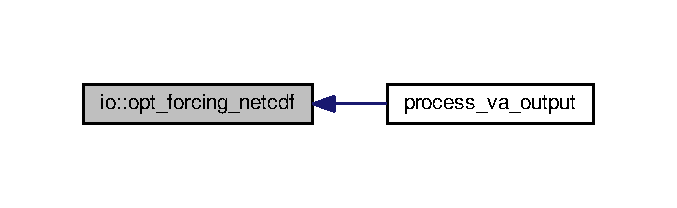
\includegraphics[width=325pt]{namespaceio_a50ab1073758d8d341087a0755354011d_icgraph}
\end{center}
\end{figure}


\index{io@{io}!opt\+\_\+vht\+\_\+netcdf@{opt\+\_\+vht\+\_\+netcdf}}
\index{opt\+\_\+vht\+\_\+netcdf@{opt\+\_\+vht\+\_\+netcdf}!io@{io}}
\subsubsection[{\texorpdfstring{opt\+\_\+vht\+\_\+netcdf(\+O\+U\+T\+P\+U\+T\+F\+I\+L\+E, I\+N\+S\+T\+R\+U\+M\+E\+N\+T, N\+V, N\+P, N\+S\+T, N\+T, V, P, S\+T, T, D)}{opt_vht_netcdf(OUTPUTFILE, INSTRUMENT, NV, NP, NST, NT, V, P, ST, T, D)}}]{\setlength{\rightskip}{0pt plus 5cm}subroutine io\+::opt\+\_\+vht\+\_\+netcdf (
\begin{DoxyParamCaption}
\item[{character (len=$\ast$), intent(in)}]{O\+U\+T\+P\+U\+T\+F\+I\+LE, }
\item[{character (len=$\ast$), intent(in)}]{I\+N\+S\+T\+R\+U\+M\+E\+NT, }
\item[{integer (kind=ik4), intent(in)}]{NV, }
\item[{integer (kind=ik4), intent(in)}]{NP, }
\item[{integer (kind=ik4), intent(in)}]{N\+ST, }
\item[{integer (kind=ik4), intent(in)}]{NT, }
\item[{character (len=$\ast$), dimension(nv), intent(in)}]{V, }
\item[{real (kind=rk8), dimension(np), intent(in)}]{P, }
\item[{character (len=$\ast$), dimension(nst), intent(in)}]{ST, }
\item[{real (kind=rk8), dimension(nt), intent(in)}]{T, }
\item[{real (kind=rk8), dimension(nv,np,nst,nt), intent(in)}]{D}
\end{DoxyParamCaption}
)}\hypertarget{namespaceio_a1feb605e982e6696d29a63e635b8d3e1}{}\label{namespaceio_a1feb605e982e6696d29a63e635b8d3e1}


Definition at line 265 of file io.\+f90.


\begin{DoxyCode}
265     \textcolor{keywordtype}{USE }\hyperlink{namespaceportable}{portable}
266     \textcolor{keywordtype}{USE }netcdf
267 
268     \textcolor{keywordtype}{IMPLICIT NONE}
269 
270     \textcolor{keywordtype}{CHARACTER (LEN=*)}, \textcolor{keywordtype}{INTENT(IN)}                                       :: outputfile   \textcolor{comment}{! Name of the
       output file.}
271     \textcolor{keywordtype}{CHARACTER (LEN=*)}, \textcolor{keywordtype}{INTENT(IN)}                                       :: instrument   \textcolor{comment}{! Instrument name.}
272     \textcolor{keywordtype}{INTEGER (KIND=IK4)}, \textcolor{keywordtype}{INTENT(IN)}                                      :: nv           \textcolor{comment}{! Number of
       variables?}
273     \textcolor{keywordtype}{INTEGER (KIND=IK4)}, \textcolor{keywordtype}{INTENT(IN)}                                      :: np           \textcolor{comment}{! Number of
       pressure levels.}
274     \textcolor{keywordtype}{INTEGER (KIND=IK4)}, \textcolor{keywordtype}{INTENT(IN)}                                      :: nst          \textcolor{comment}{! Number of
       stations.}
275     \textcolor{keywordtype}{INTEGER (KIND=IK4)}, \textcolor{keywordtype}{INTENT(IN)}                                      :: nt           \textcolor{comment}{! Number of time
       steps.}
276     \textcolor{keywordtype}{CHARACTER (LEN=*)}, \textcolor{keywordtype}{DIMENSION(NV)},  \textcolor{keywordtype}{INTENT(IN)}                       :: v            \textcolor{comment}{! Variable names?}
277     \textcolor{keywordtype}{REAL (KIND=RK8)}, \textcolor{keywordtype}{DIMENSION(NP)}, \textcolor{keywordtype}{INTENT(IN)}                          :: p            \textcolor{comment}{! Values of the
       pressure levels.}
278     \textcolor{keywordtype}{CHARACTER (LEN=*)}, \textcolor{keywordtype}{DIMENSION(NST)}, \textcolor{keywordtype}{INTENT(IN)}                       :: st           \textcolor{comment}{! Station names?}
279     \textcolor{keywordtype}{REAL (KIND=RK8)}, \textcolor{keywordtype}{DIMENSION(NT)}, \textcolor{keywordtype}{INTENT(IN)}                          :: t            \textcolor{comment}{! Time values?}
280     \textcolor{keywordtype}{REAL (KIND=RK8)}, \textcolor{keywordtype}{DIMENSION(NV,NP,NST,NT)}, \textcolor{keywordtype}{INTENT(IN)}                :: d            \textcolor{comment}{! The data.}
281 
282     \textcolor{comment}{!}
283     \textcolor{comment}{! Local variables.}
284     \textcolor{comment}{!}
285     \textcolor{keywordtype}{INTEGER (KIND=IK4)}          :: ncid                                                 \textcolor{comment}{! ID of NetCDF
       file.}
286     \textcolor{keywordtype}{INTEGER (KIND=IK4)}          :: v\_dim\_id, p\_dim\_id, st\_dim\_id, t\_dim\_id, str\_dim\_id  \textcolor{comment}{! Dimension IDs.}
287     \textcolor{keywordtype}{INTEGER (KIND=IK4)}          :: v\_var\_id, p\_var\_id, st\_var\_id, t\_var\_id, data\_var\_id \textcolor{comment}{! Variable IDs.}
288     \textcolor{keywordtype}{INTEGER (KIND=IK4)}          :: iost                                                 \textcolor{comment}{! I/O status.}
289     \textcolor{keywordtype}{INTEGER (KIND=IK4)}          :: ii                                                   \textcolor{comment}{! Counter.}
290     \textcolor{keywordtype}{INTEGER (KIND=IK4)}          :: strlen                                               \textcolor{comment}{! String length.}
291     \textcolor{keywordtype}{CHARACTER (LEN=64)}          :: tmpstr                                               \textcolor{comment}{! Temporary string.}
292 
293     iost    = nf90\_noerr
294     \textcolor{comment}{!}
295     \textcolor{comment}{! Create the NetCDF file.}
296     \textcolor{comment}{!}
297     iost    = nf90\_create(outputfile, nf90\_noclobber, ncid)
298     \textcolor{keywordflow}{IF} (iost .NE. nf90\_noerr) \textcolor{keywordflow}{GO TO} 9999
299 
300     \textcolor{comment}{!}
301     \textcolor{comment}{! Define the dimensions.}
302     \textcolor{comment}{!}
303     iost    = nf90\_def\_dim(ncid, \textcolor{stringliteral}{"variables"}, nv, v\_dim\_id)     \textcolor{comment}{! The data array contains many variables.}
304     \textcolor{keywordflow}{IF} (iost .NE. nf90\_noerr) \textcolor{keywordflow}{GO TO} 9999
305 
306     iost    = nf90\_def\_dim(ncid, \textcolor{stringliteral}{"levels"}, np, p\_dim\_id)        \textcolor{comment}{! Vertical levels.}
307     \textcolor{keywordflow}{IF} (iost .NE. nf90\_noerr) \textcolor{keywordflow}{GO TO} 9999
308 
309     iost    = nf90\_def\_dim(ncid, \textcolor{stringliteral}{"stations"}, nst, st\_dim\_id)    \textcolor{comment}{! Stations.}
310     \textcolor{keywordflow}{IF} (iost .NE. nf90\_noerr) \textcolor{keywordflow}{GO TO} 9999
311 
312     iost    = nf90\_def\_dim(ncid, \textcolor{stringliteral}{"time"}, nt, t\_dim\_id)          \textcolor{comment}{! Time steps.}
313     \textcolor{keywordflow}{IF} (iost .NE. nf90\_noerr) \textcolor{keywordflow}{GO TO} 9999
314 
315     iost    = nf90\_def\_dim(ncid, \textcolor{stringliteral}{"string"}, 64, str\_dim\_id)      \textcolor{comment}{! This dimension is used for character
       strings.}
316     \textcolor{keywordflow}{IF} (iost .NE. nf90\_noerr) \textcolor{keywordflow}{GO TO} 9999
317 
318     \textcolor{comment}{!}
319     \textcolor{comment}{! Define the variables.}
320     \textcolor{comment}{!}
321     iost    = nf90\_def\_var(ncid, \textcolor{stringliteral}{"variables"}, nf90\_char, (/ str\_dim\_id, v\_dim\_id /), v\_var\_id)
322     \textcolor{keywordflow}{IF} (iost .NE. nf90\_noerr) \textcolor{keywordflow}{GO TO} 9999
323 
324     iost    = nf90\_def\_var(ncid, \textcolor{stringliteral}{"levels"}, nf90\_double, (/ p\_dim\_id /), p\_var\_id)
325     \textcolor{keywordflow}{IF} (iost .NE. nf90\_noerr) \textcolor{keywordflow}{GO TO} 9999
326 
327     iost    = nf90\_def\_var(ncid, \textcolor{stringliteral}{"stations"}, nf90\_char, (/ str\_dim\_id, st\_dim\_id /), st\_var\_id)
328     \textcolor{keywordflow}{IF} (iost .NE. nf90\_noerr) \textcolor{keywordflow}{GO TO} 9999
329 
330     iost    = nf90\_def\_var(ncid, \textcolor{stringliteral}{"time"}, nf90\_double, (/ t\_dim\_id /), t\_var\_id)
331     \textcolor{keywordflow}{IF} (iost .NE. nf90\_noerr) \textcolor{keywordflow}{GO TO} 9999
332 
333     iost    = nf90\_def\_var(ncid, \textcolor{stringliteral}{"data"}, nf90\_double, (/ v\_dim\_id, p\_dim\_id, st\_dim\_id, t\_dim\_id /), 
      data\_var\_id)
334     \textcolor{keywordflow}{IF} (iost .NE. nf90\_noerr) \textcolor{keywordflow}{GO TO} 9999
335 
336     \textcolor{comment}{!}
337     \textcolor{comment}{! Write the instrument type as a global attribute. Make sure the string is null terminated (for C
       programs).}
338     \textcolor{comment}{!}
339     iost    = nf90\_put\_att(ncid, nf90\_global, \textcolor{stringliteral}{"instrument"}, trim(instrument)//char(0))
340     \textcolor{keywordflow}{IF} (iost .NE. nf90\_noerr) \textcolor{keywordflow}{GO TO} 9999
341 
342     \textcolor{comment}{!}
343     \textcolor{comment}{! We've finished defining stuff, leave the definition mode.}
344     \textcolor{comment}{!}
345     iost    = nf90\_enddef(ncid)
346     \textcolor{keywordflow}{IF} (iost .NE. nf90\_noerr) \textcolor{keywordflow}{GO TO} 9999
347 
348     \textcolor{comment}{!}
349     \textcolor{comment}{! Write the names of the variables. Terminate strings with a null byte, in case the data are
       subsequently read by a C program.}
350     \textcolor{comment}{!}
351     \textcolor{keywordflow}{DO} ii=1,nv
352         tmpstr  = trim(v(ii))
353         strlen  = min(63, len\_trim(tmpstr))           \textcolor{comment}{! The characters after this positon will be replaced
       by null characters.}
354         tmpstr(strlen+1:64)    = repeat(char(0), 64-strlen)
355         iost    = nf90\_put\_var(ncid, v\_var\_id, tmpstr, (/ 1, ii /), (/ 64, 1 /))
356         \textcolor{keywordflow}{IF} (iost .NE. nf90\_noerr) \textcolor{keywordflow}{GO TO} 9999
357 \textcolor{keywordflow}{    END DO}
358 
359     \textcolor{comment}{!}
360     \textcolor{comment}{! Write the names of the stations. Terminate strings with a null byte, in case the data are
       subsequently read by a C program.}
361     \textcolor{comment}{!}
362     \textcolor{keywordflow}{DO} ii=1,nst
363         tmpstr  = trim(st(ii))
364         strlen  = min(63, len\_trim(tmpstr))           \textcolor{comment}{! The characters after this positon will be replaced
       by null characters.}
365         tmpstr(strlen+1:64)    = repeat(char(0) , 64-strlen)
366         iost    = nf90\_put\_var(ncid, st\_var\_id, tmpstr, (/ 1, ii /), (/ 64, 1 /))
367         \textcolor{keywordflow}{IF} (iost .NE. nf90\_noerr) \textcolor{keywordflow}{GO TO} 9999
368 \textcolor{keywordflow}{    END DO}
369 
370     \textcolor{comment}{!}
371     \textcolor{comment}{! Write the pressure levels.}
372     \textcolor{comment}{!}
373     iost    = nf90\_put\_var(ncid, p\_var\_id, p)
374     \textcolor{keywordflow}{IF} (iost .NE. nf90\_noerr) \textcolor{keywordflow}{GO TO} 9999
375 
376     \textcolor{comment}{!}
377     \textcolor{comment}{! Write the time steps.}
378     \textcolor{comment}{!}
379     iost    = nf90\_put\_var(ncid, t\_var\_id, t)
380     \textcolor{keywordflow}{IF} (iost .NE. nf90\_noerr) \textcolor{keywordflow}{GO TO} 9999
381 
382     \textcolor{comment}{!}
383     \textcolor{comment}{! Write the big data array.}
384     \textcolor{comment}{!}
385     iost    = nf90\_put\_var(ncid, data\_var\_id, d)
386     \textcolor{keywordflow}{IF} (iost .NE. nf90\_noerr) \textcolor{keywordflow}{GO TO} 9999
387 
388     \textcolor{comment}{!}
389     \textcolor{comment}{! Close the NetCDF file.}
390     \textcolor{comment}{!}
391     iost    = nf90\_close(ncid)
392     \textcolor{keywordflow}{IF} (iost .NE. nf90\_noerr) \textcolor{keywordflow}{GO TO} 9999
393 
394     \textcolor{comment}{!}
395     \textcolor{comment}{! Catch any NetCDF errors here.}
396     \textcolor{comment}{!}
397     9999 \textcolor{keywordflow}{IF} (iost .NE. nf90\_noerr) \textcolor{keywordflow}{THEN}
398         print *,\textcolor{stringliteral}{'E: Problem creating NetCDF file '},outputfile
399         print *, trim(nf90\_strerror(iost))
400         stop \textcolor{stringliteral}{'1'}
401 \textcolor{keywordflow}{    END IF}
402 
\end{DoxyCode}


Here is the caller graph for this function\+:\nopagebreak
\begin{figure}[H]
\begin{center}
\leavevmode
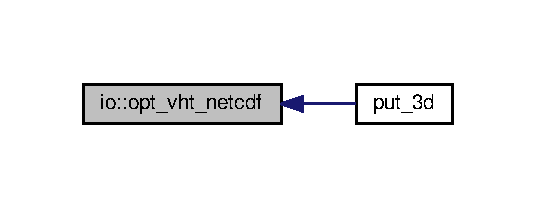
\includegraphics[width=257pt]{namespaceio_a1feb605e982e6696d29a63e635b8d3e1_icgraph}
\end{center}
\end{figure}



\hypertarget{namespacelu}{}\section{lu Module Reference}
\label{namespacelu}\index{lu@{lu}}
\subsection*{Functions/\+Subroutines}
\begin{DoxyCompactItemize}
\item 
subroutine \hyperlink{namespacelu_a578a2275703e9c18d7f262f0a3482fbe}{ludcmp} (A, N, I\+N\+DX, D, C\+O\+DE)
\item 
subroutine \hyperlink{namespacelu_a588ba20d76e8dd5c49b370d9ba3ec379}{lubksb} (A, N, I\+N\+DX, B)
\end{DoxyCompactItemize}


\subsection{Function/\+Subroutine Documentation}
\index{lu@{lu}!lubksb@{lubksb}}
\index{lubksb@{lubksb}!lu@{lu}}
\subsubsection[{\texorpdfstring{lubksb(\+A, N, I\+N\+D\+X, B)}{lubksb(A, N, INDX, B)}}]{\setlength{\rightskip}{0pt plus 5cm}subroutine lu\+::lubksb (
\begin{DoxyParamCaption}
\item[{real (kind=rk8), dimension(n,n), intent(in)}]{A, }
\item[{integer (kind=ik4)}]{N, }
\item[{integer (kind=ik4), dimension(n), intent(in)}]{I\+N\+DX, }
\item[{real (kind=rk8), dimension(n), intent(inout)}]{B}
\end{DoxyParamCaption}
)}\hypertarget{namespacelu_a588ba20d76e8dd5c49b370d9ba3ec379}{}\label{namespacelu_a588ba20d76e8dd5c49b370d9ba3ec379}


Definition at line 122 of file lu.\+f90.


\begin{DoxyCode}
122 
123 \textcolor{keywordtype}{IMPLICIT NONE}
124 \textcolor{keywordtype}{INTEGER (KIND=IK4)}                            :: n
125 \textcolor{keywordtype}{REAL (KIND=RK8)}, \textcolor{keywordtype}{DIMENSION(N,N)}, \textcolor{keywordtype}{INTENT(IN)}   :: a
126 \textcolor{keywordtype}{REAL (KIND=RK8)}, \textcolor{keywordtype}{DIMENSION(N)}, \textcolor{keywordtype}{INTENT(INOUT)}  :: b
127 \textcolor{keywordtype}{INTEGER (KIND=IK4)}, \textcolor{keywordtype}{DIMENSION(N)}, \textcolor{keywordtype}{INTENT(IN)}  :: indx
128 
129 \textcolor{comment}{!}
130 \textcolor{comment}{! Local variables.}
131 \textcolor{comment}{!}
132 \textcolor{keywordtype}{REAL (KIND=RK8)}                               :: total
133 \textcolor{keywordtype}{INTEGER (KIND=IK4)}                            :: i, j, ll, ii
134 
135 ii = 0
136 
137 \textcolor{keywordflow}{DO} i=1,n
138     ll = indx(i)
139     total = b(ll)
140     b(ll) = b(i)
141     \textcolor{keywordflow}{IF}(ii.NE.0) \textcolor{keywordflow}{THEN}
142         \textcolor{keywordflow}{DO} j=ii,i-1
143             total = total - a(i,j)*b(j)
144 \textcolor{keywordflow}{        END DO}
145     \textcolor{keywordflow}{ELSE} \textcolor{keywordflow}{IF}(total .NE. 0.0) \textcolor{keywordflow}{THEN}
146         ii = i
147 \textcolor{keywordflow}{    END IF}
148     b(i) = total
149 \textcolor{keywordflow}{END DO}
150 
151 \textcolor{keywordflow}{DO} i=n,1,-1
152     total = b(i)
153     \textcolor{keywordflow}{IF}(i < n) \textcolor{keywordflow}{THEN}
154         \textcolor{keywordflow}{DO} j=i+1,n
155             total = total - a(i,j)*b(j)
156 \textcolor{keywordflow}{        END DO}
157 \textcolor{keywordflow}{    END IF}
158     b(i) = total / a(i,i)
159 \textcolor{keywordflow}{END DO}
160 
161 \textcolor{keywordflow}{RETURN}
\end{DoxyCode}


Here is the caller graph for this function\+:\nopagebreak
\begin{figure}[H]
\begin{center}
\leavevmode
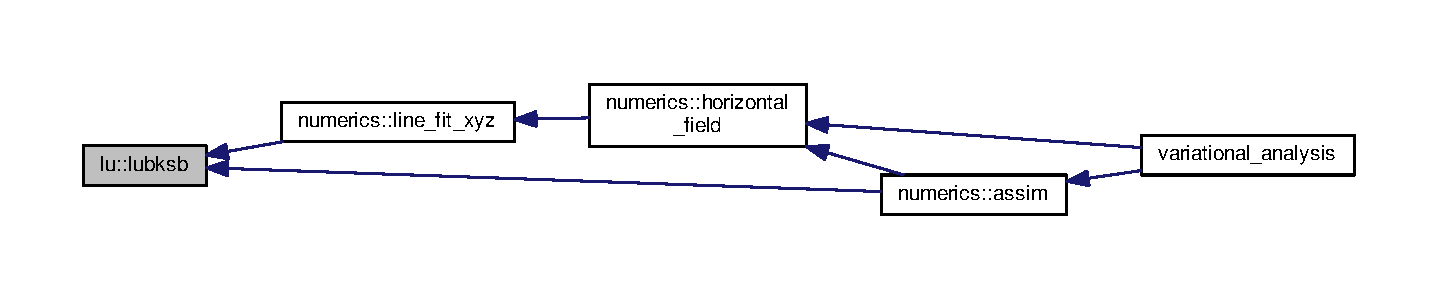
\includegraphics[width=350pt]{namespacelu_a588ba20d76e8dd5c49b370d9ba3ec379_icgraph}
\end{center}
\end{figure}


\index{lu@{lu}!ludcmp@{ludcmp}}
\index{ludcmp@{ludcmp}!lu@{lu}}
\subsubsection[{\texorpdfstring{ludcmp(\+A, N, I\+N\+D\+X, D, C\+O\+D\+E)}{ludcmp(A, N, INDX, D, CODE)}}]{\setlength{\rightskip}{0pt plus 5cm}subroutine lu\+::ludcmp (
\begin{DoxyParamCaption}
\item[{real (kind=rk8), dimension(n,n), intent(inout)}]{A, }
\item[{integer (kind=ik4), intent(in)}]{N, }
\item[{integer (kind=ik4), dimension(n), intent(out)}]{I\+N\+DX, }
\item[{integer (kind=ik4), intent(out)}]{D, }
\item[{integer (kind=ik4), intent(out)}]{C\+O\+DE}
\end{DoxyParamCaption}
)}\hypertarget{namespacelu_a578a2275703e9c18d7f262f0a3482fbe}{}\label{namespacelu_a578a2275703e9c18d7f262f0a3482fbe}


Definition at line 30 of file lu.\+f90.


\begin{DoxyCode}
30 
31 \textcolor{keywordtype}{IMPLICIT NONE}
32 \textcolor{keywordtype}{INTEGER (KIND=IK4)}, \textcolor{keywordtype}{INTENT(IN)}                  :: n        \textcolor{comment}{! The size of the array.}
33 \textcolor{keywordtype}{REAL (KIND=RK8)}, \textcolor{keywordtype}{DIMENSION(N,N)}, \textcolor{keywordtype}{INTENT(INOUT)}  :: a        \textcolor{comment}{! Array to operate on.}
34 \textcolor{keywordtype}{INTEGER (KIND=IK4)}, \textcolor{keywordtype}{DIMENSION(N)}, \textcolor{keywordtype}{INTENT(OUT)}   :: indx
35 \textcolor{keywordtype}{INTEGER (KIND=IK4)}, \textcolor{keywordtype}{INTENT(OUT)}                 :: d
36 \textcolor{keywordtype}{INTEGER (KIND=IK4)}, \textcolor{keywordtype}{INTENT(OUT)}                 :: code
37 
38 \textcolor{comment}{!}
39 \textcolor{comment}{! Local variables.}
40 \textcolor{comment}{!}
41 \textcolor{keywordtype}{INTEGER (KIND=IK4)}, \textcolor{keywordtype}{PARAMETER}                   :: nmax=100
42 \textcolor{keywordtype}{REAL (KIND=RK8)}, \textcolor{keywordtype}{PARAMETER}                      :: tiny=1.5e-16
43 \textcolor{keywordtype}{REAL (KIND=RK8)}                                 :: amax, dum, total
44 \textcolor{keywordtype}{REAL (KIND=RK8)}, \textcolor{keywordtype}{DIMENSION(NMAX)}                :: vv
45 \textcolor{keywordtype}{INTEGER (KIND=IK4)}                              :: imax
46 \textcolor{keywordtype}{INTEGER (KIND=IK4)}                              :: i, j, k                               \textcolor{comment}{! Counters.}
47 
48 d=1; code=0; 
49 imax=1          \textcolor{comment}{! Initialise IMAX so that the compiler does not complain that it is used when uninitialised
       (it never will be,}
50                 \textcolor{comment}{! but the compiler can't know that).}
51 
52 \textcolor{keywordflow}{DO} i=1,n
53     amax=0.0
54     \textcolor{keywordflow}{DO} j=1,n
55         \textcolor{keywordflow}{IF} (abs(a(i,j)).GT.amax) amax=abs(a(i,j))
56 \textcolor{keywordflow}{    END DO}
57     \textcolor{keywordflow}{IF}(amax.LT.tiny) \textcolor{keywordflow}{THEN}
58         code = 1
59         \textcolor{keywordflow}{RETURN}
60 \textcolor{keywordflow}{    END IF}
61     vv(i) = 1.0 / amax
62 \textcolor{keywordflow}{END DO}
63 
64 \textcolor{keywordflow}{DO} j=1,n
65     \textcolor{keywordflow}{DO} i=1,j-1
66         total = a(i,j)
67         \textcolor{keywordflow}{DO} k=1,i-1
68             total = total - a(i,k)*a(k,j) 
69 \textcolor{keywordflow}{        END DO}
70         a(i,j) = total
71 \textcolor{keywordflow}{    END DO}
72     amax = 0.0
73     \textcolor{keywordflow}{DO} i=j,n
74         total = a(i,j)
75         \textcolor{keywordflow}{DO} k=1,j-1
76             total = total - a(i,k)*a(k,j) 
77 \textcolor{keywordflow}{        END DO}
78         a(i,j) = total
79         dum = vv(i)*abs(total)
80         \textcolor{keywordflow}{IF}(dum.GE.amax) \textcolor{keywordflow}{THEN}
81             imax = i
82             amax = dum
83 \textcolor{keywordflow}{        END IF}
84 \textcolor{keywordflow}{    END DO}
85 
86     \textcolor{keywordflow}{IF}(j.NE.imax) \textcolor{keywordflow}{THEN}
87         \textcolor{keywordflow}{DO} k=1,n
88             dum = a(imax,k)
89             a(imax,k) = a(j,k)
90             a(j,k) = dum
91 \textcolor{keywordflow}{        END DO}
92         d = -d
93         vv(imax) = vv(j)
94 \textcolor{keywordflow}{    END IF}
95 
96     indx(j) = imax
97     \textcolor{keywordflow}{IF}(abs(a(j,j)) < tiny) a(j,j) = tiny
98 
99     \textcolor{keywordflow}{IF}(j.NE.n) \textcolor{keywordflow}{THEN}
100         dum = 1.0 / a(j,j)
101         \textcolor{keywordflow}{DO} i=j+1,n
102             a(i,j) = a(i,j)*dum
103 \textcolor{keywordflow}{        END DO}
104 \textcolor{keywordflow}{    END IF} 
105 \textcolor{keywordflow}{END DO}
106 
107 \textcolor{keywordflow}{RETURN}
\end{DoxyCode}


Here is the caller graph for this function\+:\nopagebreak
\begin{figure}[H]
\begin{center}
\leavevmode
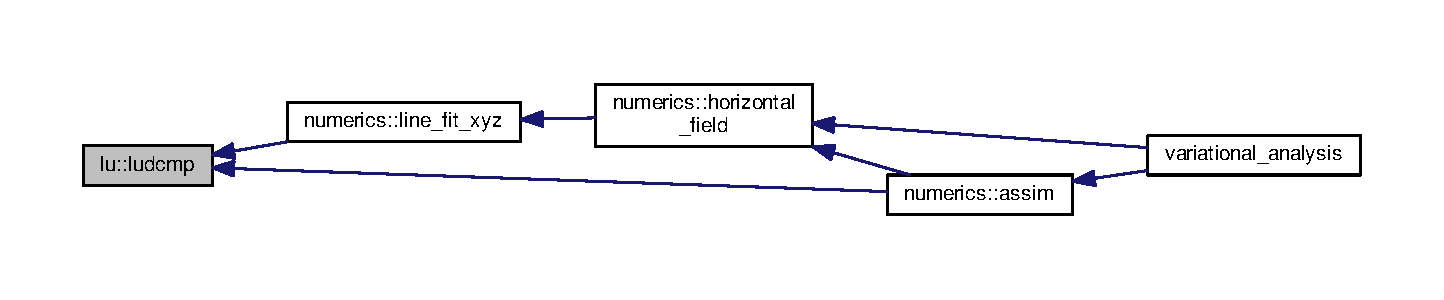
\includegraphics[width=350pt]{namespacelu_a578a2275703e9c18d7f262f0a3482fbe_icgraph}
\end{center}
\end{figure}



\hypertarget{namespacenumerics}{}\section{numerics Module Reference}
\label{namespacenumerics}\index{numerics@{numerics}}
\subsection*{Functions/\+Subroutines}
\begin{DoxyCompactItemize}
\item 
subroutine \hyperlink{namespacenumerics_ac972e0e69239cba641ad373fee101472}{itps} (KS, KB, D, DS)
\item 
subroutine \hyperlink{namespacenumerics_afbd04035bb50e63d44980bf39cf84ac3}{gmean} (MG, DP, NV, N\+ST, NT, T\+S\+M\+O\+O\+TH)
\item 
subroutine \hyperlink{namespacenumerics_a354d8c793bd1515de7af7cfa32c51389}{smooth} (A\+R\+R\+AY, N, F\+I\+L\+T\+E\+R\+\_\+\+W\+I\+D\+TH, C\+Y\+C\+L\+IC)
\item 
subroutine \hyperlink{namespacenumerics_add44a47f4f996c0266711b825fd6bb20}{caldev} (DU, KT, KS, N\+S\+TU, N\+TU, NP, N\+VU, D\+E\+V\+M2)
\item 
subroutine \hyperlink{namespacenumerics_a9581a41d0b81a5ded9690972e499c629}{horizontal\+\_\+field} (N\+ST, L\+ON, L\+AT, X, Y, F, D\+Z\+DX, D\+Z\+DY, D\+I\+VU, D\+I\+VV)
\item 
subroutine \hyperlink{namespacenumerics_a8e58d8bf1c738af1a91517fdb8b81aa2}{line\+\_\+fit\+\_\+xyz} (N, X, Y, Z, D\+Z\+DX, D\+Z\+DY, Z0)
\item 
subroutine \hyperlink{namespacenumerics_aa16b459eac85058fd1da1b9ebc4555b9}{windown} (N, X, DX, X1, L0, L1)
\item 
subroutine \hyperlink{namespacenumerics_acc1dd6ef9a4cf200fd7701143c4ae29e}{assim} (NP, DP, P, KS, KB, KT, N\+S\+TU, L\+O\+NU, L\+A\+TU, DU, N\+S\+TS, L\+O\+NS, L\+A\+TS, D\+SS, D\+I\+V\+B\+V\+AR, F\+CX, F\+CY, F\+PX, F\+PY, B\+U\+D\+G\+ET, N\+A\+D\+V\+AR, W\+V\+AR, D\+US)
\item 
subroutine \hyperlink{namespacenumerics_adbe2d748ef22c981cddde813d1db9d77}{calc\+\_\+budget\+\_\+layer} (NP, N\+TU, P, B\+U\+D\+G\+E\+T\+\_\+\+L\+A\+Y\+ER, B\+U\+D\+G\+E\+T\+\_\+\+C\+O\+L\+U\+M\+NS, A\+V\+E\+\_\+\+QS, A\+V\+E\+\_\+\+SS)
\end{DoxyCompactItemize}


\subsection{Function/\+Subroutine Documentation}
\index{numerics@{numerics}!assim@{assim}}
\index{assim@{assim}!numerics@{numerics}}
\subsubsection[{\texorpdfstring{assim(\+N\+P, D\+P, P, K\+S, K\+B, K\+T, N\+S\+T\+U, L\+O\+N\+U, L\+A\+T\+U, D\+U, N\+S\+T\+S, L\+O\+N\+S, L\+A\+T\+S, D\+S\+S, D\+I\+V\+B\+V\+A\+R, F\+C\+X, F\+C\+Y, F\+P\+X, F\+P\+Y, B\+U\+D\+G\+E\+T, N\+A\+D\+V\+A\+R, W\+V\+A\+R, D\+U\+S)}{assim(NP, DP, P, KS, KB, KT, NSTU, LONU, LATU, DU, NSTS, LONS, LATS, DSS, DIVBVAR, FCX, FCY, FPX, FPY, BUDGET, NADVAR, WVAR, DUS)}}]{\setlength{\rightskip}{0pt plus 5cm}subroutine numerics\+::assim (
\begin{DoxyParamCaption}
\item[{integer (kind=ik4), intent(in)}]{NP, }
\item[{real (kind=rk8), intent(in)}]{DP, }
\item[{real (kind=rk8), dimension(np), intent(in)}]{P, }
\item[{integer (kind=ik4), intent(in)}]{KS, }
\item[{integer (kind=ik4), intent(in)}]{KB, }
\item[{integer (kind=ik4), intent(in)}]{KT, }
\item[{integer (kind=ik4), intent(in)}]{N\+S\+TU, }
\item[{real (kind=rk8), dimension(nstu), intent(in)}]{L\+O\+NU, }
\item[{real (kind=rk8), dimension(nstu), intent(in)}]{L\+A\+TU, }
\item[{real (kind=rk8), dimension(nvu,np,nstu), intent(inout)}]{DU, }
\item[{integer (kind=ik4), intent(in)}]{N\+S\+TS, }
\item[{real (kind=rk8), dimension(nsts), intent(in)}]{L\+O\+NS, }
\item[{real (kind=rk8), dimension(nsts), intent(in)}]{L\+A\+TS, }
\item[{real (kind=rk8), dimension(nvs, nsts), intent(inout)}]{D\+SS, }
\item[{real (kind=rk8), dimension(nvbudget\+\_\+layer,np), intent(out)}]{D\+I\+V\+B\+V\+AR, }
\item[{real (kind=rk8), dimension(np), intent(out)}]{F\+CX, }
\item[{real (kind=rk8), dimension(np), intent(out)}]{F\+CY, }
\item[{real (kind=rk8), dimension(np), intent(out)}]{F\+PX, }
\item[{real (kind=rk8), dimension(np), intent(out)}]{F\+PY, }
\item[{real (kind=rk8), dimension(nvbudget\+\_\+column, ntermmax), intent(inout)}]{B\+U\+D\+G\+ET, }
\item[{integer (kind=ik4), intent(in)}]{N\+A\+D\+V\+AR, }
\item[{real (kind=rk8), dimension(5,np, nstu), intent(inout)}]{W\+V\+AR, }
\item[{real (kind=rk8), dimension(nvu,np,nstu), intent(out)}]{D\+US}
\end{DoxyParamCaption}
)}\hypertarget{namespacenumerics_acc1dd6ef9a4cf200fd7701143c4ae29e}{}\label{namespacenumerics_acc1dd6ef9a4cf200fd7701143c4ae29e}


Definition at line 429 of file numerics.\+f90.


\begin{DoxyCode}
429 \textcolor{keywordtype}{USE }\hyperlink{namespaceportable}{portable}
430 \textcolor{keywordtype}{USE }\hyperlink{namespaceconstants}{constants}
431 \textcolor{keywordtype}{USE }\hyperlink{namespacesettings}{settings}
432 \textcolor{keywordtype}{USE }\hyperlink{namespacelu}{lu}
433 \textcolor{keywordtype}{USE }\hyperlink{namespacephysics}{physics}
434 
435 \textcolor{keywordtype}{IMPLICIT NONE}
436 
437 \textcolor{keywordtype}{INTEGER (KIND=IK4)}, \textcolor{keywordtype}{INTENT(IN)}                                      :: np       \textcolor{comment}{! Number of pressure
       levels.}
438 \textcolor{keywordtype}{REAL (KIND=RK8)}, \textcolor{keywordtype}{INTENT(IN)}                                         :: dp       \textcolor{comment}{! Spacing of the pressure
       levels (Pa).}
439 \textcolor{keywordtype}{REAL (KIND=RK8)}, \textcolor{keywordtype}{DIMENSION(NP)}, \textcolor{keywordtype}{INTENT(IN)}                          :: p        \textcolor{comment}{! Pressure of each level
       (hPa)}
440 \textcolor{keywordtype}{INTEGER (KIND=IK4)}, \textcolor{keywordtype}{INTENT(IN)}                                      :: ks       \textcolor{comment}{! Index of level where the
       surface pressure is.}
441 \textcolor{keywordtype}{INTEGER (KIND=IK4)}, \textcolor{keywordtype}{INTENT(IN)}                                      :: kb       \textcolor{comment}{! Index of level where the
       surface is.}
442 \textcolor{keywordtype}{INTEGER (KIND=IK4)}, \textcolor{keywordtype}{INTENT(IN)}                                      :: kt       \textcolor{comment}{! Index of the top level.}
443 \textcolor{keywordtype}{INTEGER (KIND=IK4)}, \textcolor{keywordtype}{INTENT(IN)}                                      :: nstu     \textcolor{comment}{! Number of upper air
       stations.}
444 \textcolor{keywordtype}{REAL (KIND=RK8)}, \textcolor{keywordtype}{DIMENSION(NSTU)}, \textcolor{keywordtype}{INTENT(IN)}                        :: lonu     \textcolor{comment}{! Longitudes of the upper
       air stations}
445 \textcolor{keywordtype}{REAL (KIND=RK8)}, \textcolor{keywordtype}{DIMENSION(NSTU)}, \textcolor{keywordtype}{INTENT(IN)}                        :: latu     \textcolor{comment}{! Latitudes of the upper
       air stations}
446 \textcolor{keywordtype}{REAL (KIND=RK8)}, \textcolor{keywordtype}{DIMENSION(NVU,NP,NSTU)}, \textcolor{keywordtype}{INTENT(INOUT)}              :: du       \textcolor{comment}{! Array containing all the
       upper level data.}
447                                                                                 \textcolor{comment}{! DU(1,:,:)   = 1.0}
448                                                                                 \textcolor{comment}{! DU(2,:,:)   = rLv0/cpd}
449                                                                                 \textcolor{comment}{! DU(3,:,:)   = dry static
       energy}
450                                                                                 \textcolor{comment}{! DU(4,:,:)   = u}
451                                                                                 \textcolor{comment}{! DU(5,:,:)   = v}
452                                                                                 \textcolor{comment}{! DU(6,:,:)   = T}
453                                                                                 \textcolor{comment}{! DU(7,:,:)   = z}
454                                                                                 \textcolor{comment}{! DU(8,:,:)   = P}
455                                                                                 \textcolor{comment}{! DU(9,:,:)   = lon}
456                                                                                 \textcolor{comment}{! DU(10,:,:)  = lat}
457 \textcolor{keywordtype}{INTEGER (KIND=IK4)}, \textcolor{keywordtype}{INTENT(IN)}                                      :: nsts     \textcolor{comment}{! Number of surface level
       stations}
458 \textcolor{keywordtype}{REAL (KIND=RK8)}, \textcolor{keywordtype}{DIMENSION(NSTS)}, \textcolor{keywordtype}{INTENT(IN)}                        :: lons     \textcolor{comment}{! Longitudes of the surface
       stations.}
459 \textcolor{keywordtype}{REAL (KIND=RK8)}, \textcolor{keywordtype}{DIMENSION(NSTS)}, \textcolor{keywordtype}{INTENT(IN)}                        :: lats     \textcolor{comment}{! Latitudes of the surface
       stations.}
460 \textcolor{keywordtype}{REAL (KIND=RK8)}, \textcolor{keywordtype}{DIMENSION(NVS, NSTS)}, \textcolor{keywordtype}{INTENT(INOUT)}                :: dss      \textcolor{comment}{! Array containing all the
       surface level data.}
461 \textcolor{keywordtype}{REAL (KIND=RK8)}, \textcolor{keywordtype}{DIMENSION(NVBUDGET\_LAYER,NP)}, \textcolor{keywordtype}{INTENT(OUT)}          :: divbvar  \textcolor{comment}{!}
462 \textcolor{keywordtype}{REAL (KIND=RK8)}, \textcolor{keywordtype}{DIMENSION(NP)}, \textcolor{keywordtype}{INTENT(OUT)}                         :: fcx      \textcolor{comment}{!}
463 \textcolor{keywordtype}{REAL (KIND=RK8)}, \textcolor{keywordtype}{DIMENSION(NP)}, \textcolor{keywordtype}{INTENT(OUT)}                         :: fcy      \textcolor{comment}{!}
464 \textcolor{keywordtype}{REAL (KIND=RK8)}, \textcolor{keywordtype}{DIMENSION(NP)}, \textcolor{keywordtype}{INTENT(OUT)}                         :: fpx      \textcolor{comment}{!}
465 \textcolor{keywordtype}{REAL (KIND=RK8)}, \textcolor{keywordtype}{DIMENSION(NP)}, \textcolor{keywordtype}{INTENT(OUT)}                         :: fpy      \textcolor{comment}{!}
466 \textcolor{keywordtype}{REAL (KIND=RK8)}, \textcolor{keywordtype}{DIMENSION(NVBUDGET\_COLUMN, NTERMMAX)}, \textcolor{keywordtype}{INTENT(INOUT)}:: budget   \textcolor{comment}{!}
467 \textcolor{keywordtype}{INTEGER (KIND=IK4)}, \textcolor{keywordtype}{INTENT(IN)}                                      :: nadvar   \textcolor{comment}{!}
468 \textcolor{keywordtype}{REAL (KIND=RK8)}, \textcolor{keywordtype}{DIMENSION(5,NP, NSTU)}, \textcolor{keywordtype}{INTENT(INOUT)}               :: wvar     \textcolor{comment}{!}
469 \textcolor{keywordtype}{REAL (KIND=RK8)}, \textcolor{keywordtype}{DIMENSION(NVU,NP,NSTU)}, \textcolor{keywordtype}{INTENT(OUT)}                :: dus      \textcolor{comment}{!}
470 
471 \textcolor{comment}{!}
472 \textcolor{comment}{! Local variables.}
473 \textcolor{comment}{!}
474 \textcolor{keywordtype}{REAL (KIND=RK8)}, \textcolor{keywordtype}{DIMENSION(NP, NSTU)}                :: f                \textcolor{comment}{! Coriolis parameter at each
       station and level.}
475 \textcolor{keywordtype}{REAL (KIND=RK8)}, \textcolor{keywordtype}{DIMENSION(NP, NSTU)}                :: dzdx             \textcolor{comment}{! }
476 \textcolor{keywordtype}{REAL (KIND=RK8)}, \textcolor{keywordtype}{DIMENSION(NP, NSTU)}                :: dzdy             \textcolor{comment}{!}
477 \textcolor{keywordtype}{REAL (KIND=RK8)}, \textcolor{keywordtype}{DIMENSION(NP, NSTU)}                :: divu             \textcolor{comment}{!}
478 \textcolor{keywordtype}{REAL (KIND=RK8)}, \textcolor{keywordtype}{DIMENSION(NP, NSTU)}                :: divv             \textcolor{comment}{!}
479 
480 \textcolor{keywordtype}{REAL (KIND=RK8)}, \textcolor{keywordtype}{DIMENSION(NSTU)}                    :: x                \textcolor{comment}{! Cartesian x-coords of the
       stations at a single level.}
481 \textcolor{keywordtype}{REAL (KIND=RK8)}, \textcolor{keywordtype}{DIMENSION(NSTU)}                    :: y                \textcolor{comment}{! Cartesian y-coords of the
       stations at a single level.}
482 \textcolor{keywordtype}{REAL (KIND=RK8)}, \textcolor{keywordtype}{DIMENSION(NSTS)}                    :: xs               \textcolor{comment}{! Cartesian x-coords of the surface
       stations.}
483 \textcolor{keywordtype}{REAL (KIND=RK8)}, \textcolor{keywordtype}{DIMENSION(NSTS)}                    :: ys               \textcolor{comment}{! Cartesian y-coords of the surface
       stations.}
484 \textcolor{keywordtype}{REAL (KIND=RK8)}, \textcolor{keywordtype}{DIMENSION(1,NSTS)}                  :: fs               \textcolor{comment}{! Coriolis parameters of the
       surface stations.}
485 \textcolor{keywordtype}{REAL (KIND=RK8)}, \textcolor{keywordtype}{DIMENSION(1,NSTS)}                  :: dzdxs            \textcolor{comment}{! DZDX of the surface stations.}
486 \textcolor{keywordtype}{REAL (KIND=RK8)}, \textcolor{keywordtype}{DIMENSION(1,NSTS)}                  :: dzdys            \textcolor{comment}{! DZDY of the surface stations.}
487 \textcolor{keywordtype}{REAL (KIND=RK8)}, \textcolor{keywordtype}{DIMENSION(1,NSTS)}                  :: divus            \textcolor{comment}{! DIVU of the surface stations.}
488 \textcolor{keywordtype}{REAL (KIND=RK8)}, \textcolor{keywordtype}{DIMENSION(1,NSTS)}                  :: divvs            \textcolor{comment}{! DIVV of the surface stations.}
489 
490 \textcolor{keywordtype}{INTEGER (KIND=IK4)}                                  :: kk, mm, ist, mb, mb1, mvar, mad   \textcolor{comment}{! Counters.}
491 \textcolor{keywordtype}{REAL (KIND=RK8)}                                     :: two      = 2.0
492 \textcolor{keywordtype}{REAL(KIND=RK8)}, \textcolor{keywordtype}{DIMENSION(5)}                        :: ad       = 1.0   \textcolor{comment}{!}
493 \textcolor{keywordtype}{INTEGER (KIND=IK4)}                                  :: nterm            \textcolor{comment}{!}
494 
495 \textcolor{comment}{! The IDL code is messy ... these were all declared for the first time in the middle of other stuff.}
496 \textcolor{comment}{! For safety, we initialise many of the variables to 0 (unless the IDL code specifies otherwise). Actually,
       if you look at}
497 \textcolor{comment}{! the accompanying make files, you'll see I use a g95 option for initially zeroing variables when they are
       declared.}
498 
499 \textcolor{keywordtype}{REAL (KIND=RK8)}, \textcolor{keywordtype}{DIMENSION(NSTU)}                    :: unith
500 \textcolor{keywordtype}{REAL (KIND=RK8)}, \textcolor{keywordtype}{DIMENSION(NSTS)}                    :: uniths
501 \textcolor{keywordtype}{REAL (KIND=RK8)}, \textcolor{keywordtype}{DIMENSION(NP)}                      :: unitv
502 \textcolor{keywordtype}{REAL (KIND=RK8)}, \textcolor{keywordtype}{DIMENSION(NP)}                      :: unitv1
503 \textcolor{keywordtype}{REAL (KIND=RK8)}, \textcolor{keywordtype}{DIMENSION(NVBUDGET\_COLUMN)}         :: c
504 \textcolor{keywordtype}{REAL (KIND=RK8)}, \textcolor{keywordtype}{DIMENSION(NVBUDGET\_COLUMN)}         :: b
505 \textcolor{keywordtype}{REAL (KIND=RK8)}, \textcolor{keywordtype}{DIMENSION(NVBUDGET\_COLUMN, NVBUDGET\_COLUMN, NP, NSTU)}    :: dbdvar   \textcolor{comment}{! Important one.}
506 \textcolor{keywordtype}{REAL (KIND=RK8)}, \textcolor{keywordtype}{DIMENSION(NVBUDGET\_COLUMN, NVBUDGET\_COLUMN)}              :: a
507 \textcolor{keywordtype}{REAL (KIND=RK8)}, \textcolor{keywordtype}{DIMENSION(NVBUDGET\_COLUMN)}                               :: ld
508 
509 \textcolor{keywordtype}{REAL (KIND=RK8)}, \textcolor{keywordtype}{DIMENSION(NP, NSTU)}                :: bvar
510 \textcolor{keywordtype}{REAL (KIND=RK8)}, \textcolor{keywordtype}{DIMENSION(NP, NSTU)}                :: unitvar                      \textcolor{comment}{! This is called UNIT
       in the IDL code.}
511 \textcolor{keywordtype}{REAL (KIND=RK8)}, \textcolor{keywordtype}{DIMENSION(NP, NSTU)}                :: u
512 \textcolor{keywordtype}{REAL (KIND=RK8)}, \textcolor{keywordtype}{DIMENSION(NP, NSTU)}                :: v
513 \textcolor{keywordtype}{REAL (KIND=RK8)}, \textcolor{keywordtype}{DIMENSION(NP, NSTU)}                :: r
514 \textcolor{keywordtype}{REAL (KIND=RK8)}, \textcolor{keywordtype}{DIMENSION(NP, NSTU)}                :: h
515 \textcolor{keywordtype}{REAL (KIND=RK8)}, \textcolor{keywordtype}{DIMENSION(NP, NSTU)}                :: z 
516 \textcolor{keywordtype}{REAL (KIND=RK8)}, \textcolor{keywordtype}{DIMENSION(NP, NSTU)}                :: t
517 
518 \textcolor{keywordtype}{REAL (KIND=RK8)}, \textcolor{keywordtype}{DIMENSION(NP, NSTU)}                :: bvar1
519 \textcolor{keywordtype}{REAL (KIND=RK8)}, \textcolor{keywordtype}{DIMENSION(NP, NSTU)}                :: u1
520 \textcolor{keywordtype}{REAL (KIND=RK8)}, \textcolor{keywordtype}{DIMENSION(NP, NSTU)}                :: v1
521 \textcolor{keywordtype}{REAL (KIND=RK8)}, \textcolor{keywordtype}{DIMENSION(NP)}                      :: r2
522 \textcolor{keywordtype}{REAL (KIND=RK8)}, \textcolor{keywordtype}{DIMENSION(NP)}                      :: h2
523 \textcolor{keywordtype}{REAL (KIND=RK8)}, \textcolor{keywordtype}{DIMENSION(NP)}                      :: z2
524 \textcolor{keywordtype}{REAL (KIND=RK8)}, \textcolor{keywordtype}{DIMENSION(NP, NSTU)}                :: z1
525 
526 \textcolor{keywordtype}{REAL (KIND=RK8)}, \textcolor{keywordtype}{DIMENSION(1, NSTS)}                 :: bvars
527 \textcolor{keywordtype}{REAL (KIND=RK8)}, \textcolor{keywordtype}{DIMENSION(1, NSTS)}                 :: us
528 \textcolor{keywordtype}{REAL (KIND=RK8)}, \textcolor{keywordtype}{DIMENSION(1, NSTS)}                 :: vs
529 \textcolor{keywordtype}{REAL (KIND=RK8)}, \textcolor{keywordtype}{DIMENSION(1, NSTS)}                 :: zs
530 \textcolor{keywordtype}{REAL (KIND=RK8)}, \textcolor{keywordtype}{DIMENSION(1, NSTS)}                 :: ts
531 \textcolor{keywordtype}{INTEGER (KIND=IK4)}, \textcolor{keywordtype}{DIMENSION(4)}                    :: madn = (/ 4, 5, 2, 3 /) 
532 
533 \textcolor{keywordtype}{REAL (KIND=RK8)}, \textcolor{keywordtype}{DIMENSION(NAD, NAD)}                :: a1
534 \textcolor{comment}{!REAL (KIND=RK8), DIMENSION(NAD, NAD)                :: A2}
535 \textcolor{keywordtype}{REAL (KIND=RK8)}, \textcolor{keywordtype}{DIMENSION(NAD)}                     :: b1, ld1
536 \textcolor{keywordtype}{REAL (KIND=RK8)}, \textcolor{keywordtype}{DIMENSION(NP)}                      :: div1, div2               \textcolor{comment}{! Divergences, for NP
       levels.}
537 \textcolor{keywordtype}{REAL (KIND=RK8)}, \textcolor{keywordtype}{DIMENSION(1)}                       :: divs                     \textcolor{comment}{! Divergence for a single
       level.}
538 \textcolor{keywordtype}{REAL (KIND=RK8)}, \textcolor{keywordtype}{DIMENSION(NP)}                      :: fcx1, fpx1, fcy1, fpy1
539 \textcolor{keywordtype}{REAL (KIND=RK8)}, \textcolor{keywordtype}{DIMENSION(1)}                       :: fcxs, fcys, fpxs, fpys
540 \textcolor{keywordtype}{INTEGER (KIND=IK4)}                                  :: d, code
541 \textcolor{keywordtype}{INTEGER (KIND=IK4)}, \textcolor{keywordtype}{DIMENSION(NAD)}                  :: indx
542 \textcolor{keywordtype}{REAL (KIND=RK8)}, \textcolor{keywordtype}{DIMENSION(NP)}                      :: sc, rc
543 \textcolor{keywordtype}{REAL (KIND=RK8)}, \textcolor{keywordtype}{DIMENSION(NP,NSTU)}                      :: old1, old2,test1,test2               \textcolor{comment}{!
       Divergences, for NP levels.}
544 
545 \textcolor{comment}{!}
546 \textcolor{comment}{! What a lot of stuff that was ... surely it can be reduced!}
547 \textcolor{comment}{!}
548 \textcolor{comment}{! Initialise a whole lot of variables. For safety, we initialise lots of things with 0.0 (unless the IDL
       code specified otherwise).}
549 \textcolor{comment}{! This is because Fortran does not guarantee that variables will be initialised to any particular value
       when they are declared.}
550 \textcolor{comment}{!}
551 f       = 0.0
552 dzdx    = 0.0   
553 dzdy    = 0.0
554 divu    = 0.0
555 divv    = 0.0
556 x       = 0.0
557 y       = 0.0
558 xs      = 0.0
559 ys      = 0.0
560 fs      = 0.0
561 dzdxs   = 0.0
562 dzdys   = 0.0
563 divus   = 0.0
564 divvs   = 0.0
565 unith   = 1.0
566 uniths  = 1.0
567 unitv   = 0.0
568 unitv1  = 0.0
569 c       = 0.0
570 b       = 0.0
571 dbdvar  = 0.0
572 a       = 0.0
573 ld      = 0.0
574 bvar    = 0.0
575 unitvar = 0.0
576 u       = 0.0
577 v       = 0.0
578 r       = 0.0
579 h       = 0.0
580 z       = 0.0
581 t       = 0.0
582 bvar1   = 0.0
583 u1      = 0.0
584 v1      = 0.0
585 r2      = 0.0
586 h2      = 0.0
587 z2      = 0.0
588 z1      = 0.0
589 bvars   = 0.0
590 us      = 0.0
591 vs      = 0.0
592 zs      = 0.0
593 ts      = 0.0
594 a1      = 0.0
595 \textcolor{comment}{!A2      = 0.0}
596 b1      = 0.0
597 ld1     = 0.0
598 div1    = 0.0
599 div2    = 0.0
600 divs    = 0.0
601 fcx1    = 0.0
602 fpx1    = 0.0
603 fcy1    = 0.0
604 fpy1    = 0.0
605 fcxs    = 0.0
606 fcys    = 0.0
607 fpxs    = 0.0
608 fpys    = 0.0
609 d       = 0
610 code    = 0
611 indx    = 0
612 sc      = 0.0
613 rc      = 0.0
614 old1    = 0.0
615 old2    = 0.0
616 test1 = 0.0
617 test2 = 0.0
618 \textcolor{comment}{!}
619 \textcolor{comment}{! Calculate the components of the horizontal gradient and divergence at each vertical level, and at the
       surface.}
620 \textcolor{comment}{! All the temporary arrays used in the IDL procedure have been replaced by Fortran 90 array sections.
       Simplifies}
621 \textcolor{comment}{! things a bit.}
622 \textcolor{comment}{!}
623 
624 \textcolor{keywordflow}{DO} kk=kb,kt
625     \textcolor{keyword}{CALL }horizontal\_field(nstu, du(9,kk,:), du(10,kk,:), x, y, f(kk,:), dzdx(kk,:), dzdy(kk,:), divu(kk,:),
       divv(kk,:))
626 \textcolor{keywordflow}{END DO}
627 
628 \textcolor{keyword}{CALL }horizontal\_field(nsts, lons, lats, xs, ys, fs, dzdxs, dzdys, divus, divvs)
629 \textcolor{keywordflow}{DO} mm=1,5
630     wvar(mm,:,:)=wvar(mm,:,:)/ad(mm)
631 \textcolor{keywordflow}{END DO}
632 
633 \textcolor{keywordflow}{DO} mm=1,\hyperlink{namespacesettings_a78876a80ce867f4bc71866b783b6de89}{nvbudget\_column}
634     du(mm,1:np,1:nstu) = du(mm,1:np,1:nstu)*ad(mm)
635     dss(mm,1:nsts)=dss(mm,1:nsts)*ad(mm)
636     nterm=int(budget(mm,1), kind=\hyperlink{namespaceportable_aa110cf333432508140602ea192c4b2ea}{ik4})
637     budget(mm,2:nterm+2)=budget(mm,2:nterm+2)*ad(mm)
638 \textcolor{keywordflow}{END DO}
639 
640 \textcolor{comment}{!}
641 \textcolor{comment}{! Initialise more variables.}
642 \textcolor{comment}{!}
643 dus             = du
644 
645 unitv(kb:kt)    = 1.0
646 unitv1(ks:kt)   = 1.0
647 unitv1(ks)      = 0.5 + (budget(1,7) - p(ks))/dp*100.
648 unitv1(kt)      = 0.5
649 unitv(kb)       = 0.5 + (budget(1,7) - p(kb))/dp*100.
650 unitv(kt)       = 0.5
651 
652 \textcolor{comment}{!}
653 \textcolor{comment}{! Print a warning if the surface level is different than the level at which surface pressure is located
       (they should be}
654 \textcolor{comment}{! the same).}
655 \textcolor{comment}{!}
656 \textcolor{keywordflow}{IF} (kb .NE. ks) \textcolor{keywordflow}{THEN}
657     print *,\textcolor{stringliteral}{'Warning: KB different from KS. Try to make them the same'}
658 \textcolor{keywordflow}{END IF}
659 
660 \textcolor{comment}{!}
661 \textcolor{comment}{! Do more stuff.}
662 \textcolor{comment}{!}
663 \textcolor{keywordflow}{DO} mb=1,\hyperlink{namespacesettings_a78876a80ce867f4bc71866b783b6de89}{nvbudget\_column}
664     nterm   = int(budget(mb, 1), 4)
665     c(mb)   = -sum(budget(mb,3:nterm+1))
666 \textcolor{keywordflow}{END DO}
667 
668 \textcolor{comment}{!}
669 \textcolor{comment}{! Fill out UNITVAR, R, H, U, V, Z and T from the big DUS array (which was passed into this procedure as DU)}
670 \textcolor{comment}{!}
671 unitvar(kb:kt,:)    = dus(1,kb:kt,:)
672 r(kb:kt,:)          = dus(2,kb:kt,:)
673 h(kb:kt,:)          = dus(3,kb:kt,:)
674 u(kb:kt,:)          = dus(4,kb:kt,:)
675 v(kb:kt,:)          = dus(5,kb:kt,:)
676 z(kb:kt,:)          = dus(7,kb:kt,:)
677 t(kb:kt,:)          = dus(6,kb:kt,:)
678 
679 \textcolor{comment}{!}
680 \textcolor{comment}{! Fill out US, VS, ZS and TS from the big DSS array.}
681 \textcolor{comment}{!}
682 us(1,:)             = dss(4,:)
683 vs(1,:)             = dss(5,:)
684 zs(1,:)             = dss(7,:)
685 ts(1,:)             = dss(6,:)
686 
687 \textcolor{comment}{!}
688 \textcolor{comment}{! I think this is where the partial derivatives to the five constraint equations (equations (14)-(17) in
       Zhang and Lin) are}
689 \textcolor{comment}{! calculated ... maybe.}
690 \textcolor{comment}{!}
691 \textcolor{keywordflow}{DO} kk=kb,kt
692     dbdvar(1,1,kk,:)    = unitvar(kk,:)*divu(kk,:)*dp/\hyperlink{namespaceconstants_a046aef138fbc8d05251d4fdc6eb3ee89}{g}
693     dbdvar(1,2,kk,:)    = unitvar(kk,:)*divv(kk,:)*dp/\hyperlink{namespaceconstants_a046aef138fbc8d05251d4fdc6eb3ee89}{g}
694     dbdvar(2,1,kk,:)    = r(kk,:)*divu(kk,:)*dp/\hyperlink{namespaceconstants_a046aef138fbc8d05251d4fdc6eb3ee89}{g}
695     dbdvar(2,2,kk,:)    = r(kk,:)*divv(kk,:)*dp/\hyperlink{namespaceconstants_a046aef138fbc8d05251d4fdc6eb3ee89}{g}
696     dbdvar(2,3,kk,:)    = (u(kk,:)*divu(kk,:) + v(kk,:)*divv(kk,:))*dp/\hyperlink{namespaceconstants_a046aef138fbc8d05251d4fdc6eb3ee89}{g}
697     dbdvar(3,1,kk,:)    = h(kk,:)*divu(kk,:)*dp/\hyperlink{namespaceconstants_a046aef138fbc8d05251d4fdc6eb3ee89}{g}
698     dbdvar(3,2,kk,:)    = h(kk,:)*divv(kk,:)*dp/\hyperlink{namespaceconstants_a046aef138fbc8d05251d4fdc6eb3ee89}{g}
699     dbdvar(3,4,kk,:)    = (u(kk,:)*divu(kk,:) + v(kk,:)*divv(kk,:))*dp/\hyperlink{namespaceconstants_a046aef138fbc8d05251d4fdc6eb3ee89}{g}
700     dbdvar(4,1,kk,:)    = (2.0*u(kk,:)*divu(kk,:) + v(kk,:)*divv(kk,:))*dp/\hyperlink{namespaceconstants_a046aef138fbc8d05251d4fdc6eb3ee89}{g}
701     dbdvar(4,2,kk,:)    = (u(kk,:)*divv(kk,:) - f(kk,:)/nstu)*dp/\hyperlink{namespaceconstants_a046aef138fbc8d05251d4fdc6eb3ee89}{g}
702     dbdvar(4,4,kk,:)    = (kt+1-kk)*\hyperlink{namespaceconstants_ad91564da82b97ea0d29ce0565565db85}{rd}*dp/100.0/p(kk)*dzdx(kk,:)*dp/\hyperlink{namespaceconstants_a046aef138fbc8d05251d4fdc6eb3ee89}{g}
703     dbdvar(5,1,kk,:)    = (v(kk,:)*divu(kk,:) + f(kk,:)/nstu)*dp/\hyperlink{namespaceconstants_a046aef138fbc8d05251d4fdc6eb3ee89}{g}
704     dbdvar(5,2,kk,:)    = (u(kk,:)*divu(kk,:) + 2.0*v(kk,:)*divv(kk,:))*dp/\hyperlink{namespaceconstants_a046aef138fbc8d05251d4fdc6eb3ee89}{g}
705     dbdvar(5,4,kk,:)    = (kt+1-kk)*\hyperlink{namespaceconstants_ad91564da82b97ea0d29ce0565565db85}{rd}*dp/100.0/p(kk)*dzdy(kk,:)*dp/\hyperlink{namespaceconstants_a046aef138fbc8d05251d4fdc6eb3ee89}{g}
706 \textcolor{keywordflow}{END DO}
707 
708 \textcolor{keywordflow}{DO} mb=1,5                   \textcolor{comment}{! This loops over the first five variables in the dus array.}
709     bvar(kb:kt,:)       = dus(mb,kb:kt,:)
710     bvars(1,:)          = dss(mb,:)
711 
712     \textcolor{keywordflow}{DO} mb1=1,5
713         \textcolor{keywordflow}{DO} ist=1,nstu
714             \textcolor{keywordflow}{DO} kk=kb,kt
715                 u1(kk,ist)  = -dbdvar(mb1,1,kk,ist)/two/wvar(4,kk,ist)
716                 v1(kk,ist)  = -dbdvar(mb1,2,kk,ist)/two/wvar(5,kk,ist)
717                 r2(kk)      = 0.0
718                 h2(kk)      = -dbdvar(mb1,4,kk,ist)/two/wvar(3,kk,ist)
719                 test1(kk,ist)=-wvar(4,kk,ist)
720                 test2(kk,ist)=-wvar(5,kk,ist)
721 \textcolor{keywordflow}{            END DO}
722             \textcolor{keyword}{CALL }\hyperlink{namespacephysics_a0ca41ce81224f2d7b292dc474c080c60}{height}(np, kb, kt, p, h2, r2, z2)
723             z1(:,ist)       = z2(:)
724 \textcolor{keywordflow}{        END DO}
725         \textcolor{keyword}{CALL }\hyperlink{namespacephysics_adc35216d512f6586071a79fba286a39c}{diverg}(unith=unith, var=bvar, u=u1, v=v1, divu=divu, divv=divv, div1=div2)
726         a(mb,mb1)           = dot\_product(div2,unitv)*dp/\hyperlink{namespaceconstants_a046aef138fbc8d05251d4fdc6eb3ee89}{g}          \textcolor{comment}{! Equivalent to IDL code:
       transpose(div2)#unitv*dp/g}
727         \textcolor{comment}{!}
728         \textcolor{comment}{! Print a warning if ABS(MB,MB1) is greater than 100.}
729         \textcolor{comment}{!}
730         \textcolor{comment}{!IF (ABS(A(MB,MB1)) .GT. 100) THEN}
731             \textcolor{comment}{!PRINT *,'Warning: A(MB,MB1) > 100',MB,MB1,A(MB,MB1)!,DIV2,'..',UNITV ,'..',DP,'..',G}
732             \textcolor{comment}{!  print *, OLD1,'....',test1,'#',MB1}
733             \textcolor{comment}{!  print *, OLD2,'....',test2,'#',MB1}
734         \textcolor{comment}{!else}
735         \textcolor{comment}{!    print *, U1,'...#....',V1}
736         \textcolor{comment}{!END IF}
737         old1=test1
738         old2=test2
739         \textcolor{comment}{!}
740         \textcolor{comment}{! Calculate extra stuff for MB=4}
741         \textcolor{comment}{!}
742         \textcolor{keywordflow}{IF} (mb .EQ. 4) \textcolor{keywordflow}{THEN}
743             \textcolor{keyword}{CALL }\hyperlink{namespacephysics_a56a179b5bd2c13a2201b2367037a42cf}{fcorlx}(unith, nstu, f, v1, fcx1)
744             \textcolor{keyword}{CALL }\hyperlink{namespacephysics_acf841366af6f4fd7502b4031a2cacb56}{fpgd}(unith, z1, dzdx, fpx1)
745             a(4,mb1)    = a(4,mb1) - dot\_product(fcx1,unitv)*dp/\hyperlink{namespaceconstants_a046aef138fbc8d05251d4fdc6eb3ee89}{g} - dot\_product(fpx1,unitv)*dp/
      \hyperlink{namespaceconstants_a046aef138fbc8d05251d4fdc6eb3ee89}{g}
746 \textcolor{keywordflow}{        END IF}
747 
748         \textcolor{comment}{!}
749         \textcolor{comment}{! Calculate extra stuff for MB=5}
750         \textcolor{comment}{!}
751         \textcolor{keywordflow}{IF} (mb .EQ. 5) \textcolor{keywordflow}{THEN}
752             \textcolor{keyword}{CALL }\hyperlink{namespacephysics_a1f64bd544ea55c7fbbf5330725fc0896}{fcorly}(unith, nstu, f, u1, fcy1)
753             \textcolor{keyword}{CALL }\hyperlink{namespacephysics_acf841366af6f4fd7502b4031a2cacb56}{fpgd}(unith, z1, dzdy, fpy1)
754             a(5,mb1)    = a(5,mb1) - dot\_product(fcy1,unitv)*dp/\hyperlink{namespaceconstants_a046aef138fbc8d05251d4fdc6eb3ee89}{g} - dot\_product(fpy1,unitv)*dp/
      \hyperlink{namespaceconstants_a046aef138fbc8d05251d4fdc6eb3ee89}{g}
755 \textcolor{keywordflow}{        END IF}
756 \textcolor{keywordflow}{    END DO}
757 
758     \textcolor{keyword}{CALL }\hyperlink{namespacephysics_adc35216d512f6586071a79fba286a39c}{diverg}(unith, bvar, u, v, divu, divv, div1)
759     \textcolor{keyword}{CALL }\hyperlink{namespacephysics_adc35216d512f6586071a79fba286a39c}{diverg}(uniths, bvars, us, vs, divus, divvs, divs)
760     \textcolor{keyword}{CALL }itps(ks, kb, div1, divs(1))
761     divbvar(mb,ks:kt)   = div1(ks:kt)/ad(mb)
762     b(mb)               = dot\_product(div1,unitv1)*dp/\hyperlink{namespaceconstants_a046aef138fbc8d05251d4fdc6eb3ee89}{g} + c(mb)
763     nterm               = int(budget(mb, 1), kind=\hyperlink{namespaceportable_aa110cf333432508140602ea192c4b2ea}{ik4})
764     budget(mb, nterm+2) = -dot\_product(div1,unitv1)*dp/\hyperlink{namespaceconstants_a046aef138fbc8d05251d4fdc6eb3ee89}{g}
765 \textcolor{keywordflow}{END DO}
766 
767 \textcolor{keyword}{CALL }\hyperlink{namespacephysics_adc35216d512f6586071a79fba286a39c}{diverg}(unith, t, u, v, divu, divv, div1)
768 \textcolor{keyword}{CALL }\hyperlink{namespacephysics_adc35216d512f6586071a79fba286a39c}{diverg}(uniths, ts, us, vs, divus, divvs, divs)
769 \textcolor{keyword}{CALL }itps(ks, kb, div1, divs(1))
770 divbvar(6,ks:kt)        = div1(ks:kt)
771 
772 \textcolor{keywordflow}{DO} mvar=1,nadvar
773     mm  = madn(mvar)
774     \textcolor{keywordflow}{DO} mb1=1,5
775         bvar1(kb:kt,:)  = -dbdvar(mb1,mvar,kb:kt,:)/2.0/wvar(mm,kb:kt,:)
776         \textcolor{keyword}{CALL }\hyperlink{namespacephysics_adc35216d512f6586071a79fba286a39c}{diverg}(unith, bvar1, u, v, divu, divv, div1)
777         a(mm,mb1)       = a(mm,mb1) + dot\_product(div1,unitv)*dp/\hyperlink{namespaceconstants_a046aef138fbc8d05251d4fdc6eb3ee89}{g}
778 \textcolor{keywordflow}{    END DO}
779 \textcolor{keywordflow}{END DO}
780 
781 \textcolor{keyword}{CALL }\hyperlink{namespacephysics_a56a179b5bd2c13a2201b2367037a42cf}{fcorlx}(unith, nstu, f, v, fcx1)
782 \textcolor{keyword}{CALL }\hyperlink{namespacephysics_a56a179b5bd2c13a2201b2367037a42cf}{fcorlx}(uniths, nsts, fs, vs, fcxs)
783 \textcolor{keyword}{CALL }itps(ks, kb, fcx1, fcxs(1))
784 budget(4,6)     = dot\_product(fcx1,unitv1)*dp/\hyperlink{namespaceconstants_a046aef138fbc8d05251d4fdc6eb3ee89}{g}
785 
786 \textcolor{keyword}{CALL }\hyperlink{namespacephysics_acf841366af6f4fd7502b4031a2cacb56}{fpgd}(unith, z, dzdx, fpx1)
787 \textcolor{keyword}{CALL }\hyperlink{namespacephysics_acf841366af6f4fd7502b4031a2cacb56}{fpgd}(uniths, zs, dzdxs, fpxs)
788 \textcolor{keyword}{CALL }itps(ks, kb, fpx1, fpxs(1))
789 budget(4,7)     = dot\_product(fpx1,unitv1)*dp/\hyperlink{namespaceconstants_a046aef138fbc8d05251d4fdc6eb3ee89}{g}
790 b(4)            = b(4) - budget(4,6) - budget(4,7)
791 
792 \textcolor{keyword}{CALL }\hyperlink{namespacephysics_a1f64bd544ea55c7fbbf5330725fc0896}{fcorly}(unith, nstu, f, u, fcy1)
793 \textcolor{keyword}{CALL }\hyperlink{namespacephysics_a1f64bd544ea55c7fbbf5330725fc0896}{fcorly}(uniths, nsts, fs, us, fcys)
794 \textcolor{keyword}{CALL }itps(ks, kb, fcy1, fcys(1))
795 budget(5,6)     = dot\_product(fcy1,unitv1)*dp/\hyperlink{namespaceconstants_a046aef138fbc8d05251d4fdc6eb3ee89}{g}
796 
797 \textcolor{keyword}{CALL }\hyperlink{namespacephysics_acf841366af6f4fd7502b4031a2cacb56}{fpgd}(unith, z, dzdy, fpy1)
798 \textcolor{keyword}{CALL }\hyperlink{namespacephysics_acf841366af6f4fd7502b4031a2cacb56}{fpgd}(uniths, zs, dzdys, fpys)
799 \textcolor{keyword}{CALL }itps(ks, kb, fpy1, fpys(1))
800 budget(5,7)     = dot\_product(fpy1,unitv1)*dp/\hyperlink{namespaceconstants_a046aef138fbc8d05251d4fdc6eb3ee89}{g}
801 b(5)            = b(5) - budget(5,6) - budget(5,7)
802 
803 fcx             = fcx1
804 fcy             = fcy1
805 fpx             = fpx1
806 fpy             = fpy1
807 
808 budget(1:5,2)   = -b(1:5)
809 b               = -b
810 
811 a1              = 0.0
812 b1              = 0.0
813 a1(1:\hyperlink{namespacesettings_a4f624be133b88a44c8976b47b85e8eec}{nad},1:\hyperlink{namespacesettings_a4f624be133b88a44c8976b47b85e8eec}{nad}) = a(1:\hyperlink{namespacesettings_a4f624be133b88a44c8976b47b85e8eec}{nad},1:\hyperlink{namespacesettings_a4f624be133b88a44c8976b47b85e8eec}{nad})
814 b1(1:\hyperlink{namespacesettings_a4f624be133b88a44c8976b47b85e8eec}{nad})       = b(1:\hyperlink{namespacesettings_a4f624be133b88a44c8976b47b85e8eec}{nad})
815 \textcolor{comment}{!A2              = A1}
816 
817 \textcolor{keywordflow}{IF} (\hyperlink{namespacesettings_a4f624be133b88a44c8976b47b85e8eec}{nad} .LT. 3 ) \textcolor{keywordflow}{THEN}
818     ld1(1)  = b1(1)/a1(1,1)
819 \textcolor{keywordflow}{ELSE}
820     \textcolor{keyword}{CALL }\hyperlink{namespacelu_a578a2275703e9c18d7f262f0a3482fbe}{ludcmp}(a=a1, n=\hyperlink{namespacesettings_a4f624be133b88a44c8976b47b85e8eec}{nad}, indx=indx, d=d, code=code)
821     \textcolor{keyword}{CALL }\hyperlink{namespacelu_a588ba20d76e8dd5c49b370d9ba3ec379}{lubksb}(a=a1, n=\hyperlink{namespacesettings_a4f624be133b88a44c8976b47b85e8eec}{nad}, indx=indx, b=b1)
822     ld1     = b1
823 \textcolor{keywordflow}{ENDIF}
824 
825 ld(1:\hyperlink{namespacesettings_a4f624be133b88a44c8976b47b85e8eec}{nad})   = ld1(1:\hyperlink{namespacesettings_a4f624be133b88a44c8976b47b85e8eec}{nad})
826 
827 \textcolor{comment}{!}
828 \textcolor{comment}{! I think this is where equation (24) in Zhang and Lin is implemented.}
829 \textcolor{comment}{!}
830 
831 \textcolor{keywordflow}{DO} mad=1,nadvar
832     mm = madn(mad)
833     \textcolor{keywordflow}{DO} mb=1,\hyperlink{namespacesettings_a4f624be133b88a44c8976b47b85e8eec}{nad}
834         \textcolor{keywordflow}{if} (mm .eq. 3) \textcolor{keywordflow}{then}
835 \textcolor{keywordflow}{        endif}
836         dus(mm,kb:kt,1:nstu)    = dus(mm,kb:kt,1:nstu) - ld(mb)*dbdvar(mb,mad,kb:kt,1:nstu)/2.0/wvar(mm,kb:
      kt,1:nstu)
837 \textcolor{keywordflow}{    END DO}
838 \textcolor{keywordflow}{END DO}
839 
840 \textcolor{comment}{!}
841 \textcolor{comment}{! Update T and Z based on s and r. This comment is copied directly from IDL code.}
842 \textcolor{comment}{!}
843 \textcolor{keywordflow}{DO} ist=1,nstu
844     sc(1:np)    = dus(3,1:np,ist)
845     rc(1:np)    = dus(2,1:np,ist)*\hyperlink{namespaceconstants_a32354adf3493f59d0fc17b0302b2c368}{cpd}/\hyperlink{namespaceconstants_afb3befdfd57058ee9d073b832134a601}{lv0}
846     rc(1)       = dss(2,ist)*\hyperlink{namespaceconstants_a32354adf3493f59d0fc17b0302b2c368}{cpd}/\hyperlink{namespaceconstants_afb3befdfd57058ee9d073b832134a601}{lv0}
847     sc(1)       = dss(3,ist)
848     \textcolor{keyword}{CALL }\hyperlink{namespacephysics_a3f1959e7b3ff1a8d052f1e0441b1c379}{s\_r\_to\_t\_z}(p, dss(8,ist), dss(7,ist), sc, rc, dus(6,1:np,ist), dus(7,1:np,ist))
849 \textcolor{keywordflow}{END DO}
850 
851 \textcolor{keywordflow}{DO} mm=1,\hyperlink{namespacesettings_a78876a80ce867f4bc71866b783b6de89}{nvbudget\_column}
852     dus(mm,1:np,1:nstu)     = dus(mm,1:np,1:nstu)/ad(mm)
853     nterm   = int(budget(mm,1), kind=\hyperlink{namespaceportable_aa110cf333432508140602ea192c4b2ea}{ik4})
854     budget(mm,2:nterm+2)    = budget(mm,2:nterm+2)/ad(mm)
855 \textcolor{keywordflow}{END DO}
856 
\end{DoxyCode}


Here is the call graph for this function\+:\nopagebreak
\begin{figure}[H]
\begin{center}
\leavevmode
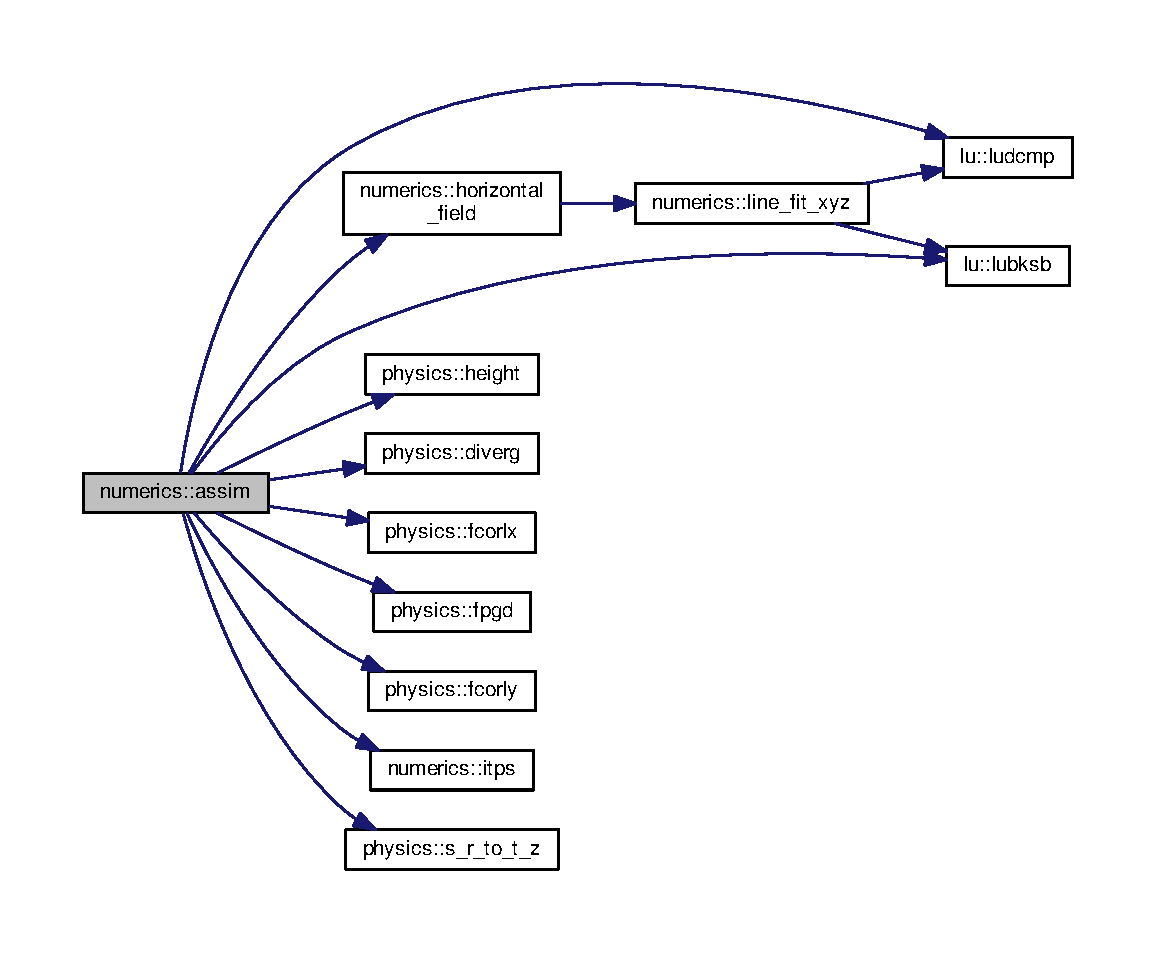
\includegraphics[width=350pt]{namespacenumerics_acc1dd6ef9a4cf200fd7701143c4ae29e_cgraph}
\end{center}
\end{figure}




Here is the caller graph for this function\+:\nopagebreak
\begin{figure}[H]
\begin{center}
\leavevmode
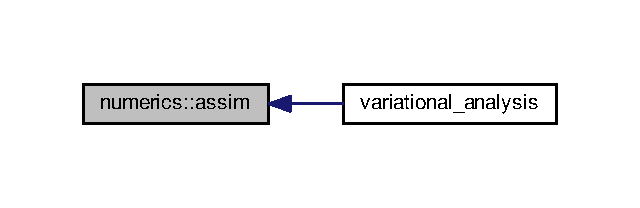
\includegraphics[width=307pt]{namespacenumerics_acc1dd6ef9a4cf200fd7701143c4ae29e_icgraph}
\end{center}
\end{figure}


\index{numerics@{numerics}!calc\+\_\+budget\+\_\+layer@{calc\+\_\+budget\+\_\+layer}}
\index{calc\+\_\+budget\+\_\+layer@{calc\+\_\+budget\+\_\+layer}!numerics@{numerics}}
\subsubsection[{\texorpdfstring{calc\+\_\+budget\+\_\+layer(\+N\+P, N\+T\+U, P, B\+U\+D\+G\+E\+T\+\_\+\+L\+A\+Y\+E\+R, B\+U\+D\+G\+E\+T\+\_\+\+C\+O\+L\+U\+M\+N\+S, A\+V\+E\+\_\+\+Q\+S, A\+V\+E\+\_\+\+S\+S)}{calc_budget_layer(NP, NTU, P, BUDGET_LAYER, BUDGET_COLUMNS, AVE_QS, AVE_SS)}}]{\setlength{\rightskip}{0pt plus 5cm}subroutine numerics\+::calc\+\_\+budget\+\_\+layer (
\begin{DoxyParamCaption}
\item[{integer (kind=ik4), intent(in)}]{NP, }
\item[{integer (kind=ik4), intent(in)}]{N\+TU, }
\item[{real (kind=rk8), dimension(np), intent(in)}]{P, }
\item[{real (kind=rk8), dimension(nvbudget\+\_\+layer,ntermmaxv,np,ntu), intent(inout)}]{B\+U\+D\+G\+E\+T\+\_\+\+L\+A\+Y\+ER, }
\item[{real (kind=rk8), dimension(nvbudget\+\_\+column,ntermmax,ntu), intent(in)}]{B\+U\+D\+G\+E\+T\+\_\+\+C\+O\+L\+U\+M\+NS, }
\item[{real (kind=rk8), dimension(ntu), intent(in)}]{A\+V\+E\+\_\+\+QS, }
\item[{real (kind=rk8), dimension(ntu), intent(in)}]{A\+V\+E\+\_\+\+SS}
\end{DoxyParamCaption}
)}\hypertarget{namespacenumerics_adbe2d748ef22c981cddde813d1db9d77}{}\label{namespacenumerics_adbe2d748ef22c981cddde813d1db9d77}


Definition at line 869 of file numerics.\+f90.


\begin{DoxyCode}
869 \textcolor{keywordtype}{USE }\hyperlink{namespaceportable}{portable}
870 \textcolor{keywordtype}{USE }\hyperlink{namespaceconstants}{constants}
871 \textcolor{keywordtype}{USE }\hyperlink{namespacesettings}{settings}
872 
873 \textcolor{keywordtype}{IMPLICIT NONE}
874 
875 \textcolor{keywordtype}{INTEGER (KIND=IK4)}, \textcolor{keywordtype}{INTENT(IN)}                                              :: np               \textcolor{comment}{! Number of
       pressure levels.}
876 \textcolor{keywordtype}{INTEGER (KIND=IK4)}, \textcolor{keywordtype}{INTENT(IN)}                                              :: ntu              \textcolor{comment}{! Number of
       times.}
877 \textcolor{keywordtype}{REAL (KIND=RK8)}, \textcolor{keywordtype}{DIMENSION(NP)}, \textcolor{keywordtype}{INTENT(IN)}                                  :: p                \textcolor{comment}{! Pressure
       of each level (hPa)}
878 \textcolor{keywordtype}{REAL (KIND=RK8)}, \textcolor{keywordtype}{DIMENSION(NTU)}, \textcolor{keywordtype}{INTENT(IN)}                                 :: ave\_qs
879 \textcolor{keywordtype}{REAL (KIND=RK8)}, \textcolor{keywordtype}{DIMENSION(NTU)}, \textcolor{keywordtype}{INTENT(IN)}                                 :: ave\_ss
880 \textcolor{keywordtype}{REAL (KIND=RK8)}, \textcolor{keywordtype}{DIMENSION(NVBUDGET\_COLUMN,NTERMMAX,NTU)}, \textcolor{keywordtype}{INTENT(IN)}        :: budget\_columns
881 \textcolor{keywordtype}{REAL (KIND=RK8)}, \textcolor{keywordtype}{DIMENSION(NVBUDGET\_LAYER,NTERMMAXV,NP,NTU)}, \textcolor{keywordtype}{INTENT(INOUT)}  :: budget\_layer
882 
883 \textcolor{comment}{!}
884 \textcolor{comment}{! Local variables.}
885 \textcolor{comment}{!}
886 \textcolor{keywordtype}{REAL (KIND=RK8)}                                                     :: dp               \textcolor{comment}{! Vertical
       resolution (hPa)}
887 \textcolor{keywordtype}{REAL (KIND=RK8)}                                                     :: dp2
888 \textcolor{keywordtype}{REAL (KIND=RK8)}, \textcolor{keywordtype}{DIMENSION(6,NP+1)}                                  :: omega\_vb
889 
890 \textcolor{keywordtype}{INTEGER (KIND=IK4)}                                                  :: ks               \textcolor{comment}{! Index of surface
       level.}
891 \textcolor{keywordtype}{INTEGER (KIND=IK4)}                                                  :: kt               \textcolor{comment}{! Index of top
       level.}
892 \textcolor{keywordtype}{INTEGER (KIND=IK4)}                                                  :: k1, k2
893 \textcolor{keywordtype}{INTEGER (KIND=IK4)}                                                  :: nterm
894 
895 \textcolor{keywordtype}{INTEGER (KIND=IK4)}                                                  :: kk,ll,mvb,iterm  \textcolor{comment}{! Counters.}
896 
897 \textcolor{comment}{!}
898 \textcolor{comment}{! Calculate vertical resolution.}
899 \textcolor{comment}{!}
900 dp  = p(1) - p(2)
901 
902 \textcolor{keywordflow}{DO} ll=2,ntu-1
903     ks  = int(budget\_layer(1,2,1,ll), kind=\hyperlink{namespaceportable_aa110cf333432508140602ea192c4b2ea}{ik4})
904     kt  = int(budget\_layer(1,4,1,ll), kind=\hyperlink{namespaceportable_aa110cf333432508140602ea192c4b2ea}{ik4})
905 
906     omega\_vb = 0.0
907     omega\_vb(1,ks)  = -budget\_columns(1,3,ll)*\hyperlink{namespaceconstants_a046aef138fbc8d05251d4fdc6eb3ee89}{g}/100.0                                   \textcolor{comment}{! hPa/s}
908 
909     \textcolor{keywordflow}{DO} kk=ks,kt
910         budget\_layer(1,4,kk,ll) = -budget\_layer(1,3,kk,ll)                              \textcolor{comment}{! -dw/dp}
911         dp2                     = dp
912         \textcolor{keywordflow}{IF} (kk .EQ. ks) dp2     = (budget\_columns(1,7,ll) - p(ks)) + 0.5*dp
913         \textcolor{keywordflow}{IF} (kk .EQ. kt) dp2     = 0.5*dp
914         omega\_vb(1,kk+1)        = omega\_vb(1,kk) + budget\_layer(1,4,kk,ll)*dp2          \textcolor{comment}{! DP2 vertically
       integrated not zero.}
915 \textcolor{keywordflow}{    END DO}
916 
917     \textcolor{keywordflow}{DO} mvb=2,6
918         \textcolor{keywordflow}{DO} kk=ks,kt+1
919             k1                  = max(ks, kk-1)
920             k2                  = min(kt,kk)
921             omega\_vb(mvb,kk)    = omega\_vb(1,kk) * (budget\_layer(mvb,1,k1,ll) + budget\_layer(mvb,1,k2,ll))*
      0.5
922 \textcolor{keywordflow}{        END DO}
923 \textcolor{keywordflow}{    END DO}
924 
925     kk                  = ks
926     mvb                 = 2
927     omega\_vb(mvb,kk)    = omega\_vb(1,kk)*ave\_qs(ll)
928     mvb                 = 3
929     omega\_vb(mvb,kk)    = omega\_vb(1,kk)*ave\_ss(ll)
930 
931     \textcolor{keywordflow}{DO} mvb=1,6
932         nterm                               = int(budget\_layer(mvb,1,1,1), kind=
      \hyperlink{namespaceportable_aa110cf333432508140602ea192c4b2ea}{ik4})
933         \textcolor{keywordflow}{DO} kk=ks,kt
934             budget\_layer(mvb,nterm+3,kk,ll) = 0.5*(omega\_vb(mvb,kk) + omega\_vb(mvb,kk+1))
935 \textcolor{keywordflow}{        END DO}
936         budget\_layer(mvb,nterm+3,kt,ll)     = omega\_vb(mvb,kt+1)
937 \textcolor{keywordflow}{    END DO}
938 
939     \textcolor{comment}{!}
940     \textcolor{comment}{! Vertical flux advection.}
941     \textcolor{comment}{!}
942     \textcolor{keywordflow}{DO} mvb=1,6
943         nterm                               = int(budget\_layer(mvb,1,1,1), kind=
      \hyperlink{namespaceportable_aa110cf333432508140602ea192c4b2ea}{ik4})
944         \textcolor{keywordflow}{DO} kk=ks,kt
945             budget\_layer(mvb,4,kk,ll)       = -(omega\_vb(mvb,kk) - omega\_vb(mvb,kk+1))/dp
946 \textcolor{keywordflow}{        END DO}
947         dp2                                 = 0.5*dp
948         budget\_layer(mvb,4,kt,ll)           = -(omega\_vb(mvb,kt) - omega\_vb(mvb,kt+1))/dp2
949         dp2                                 = 0.5*dp + (budget\_columns(1,7,ll) - p(ks))
950         budget\_layer(mvb,4,ks,ll)           = -(omega\_vb(mvb,ks) - omega\_vb(mvb,ks+1))/dp2
951 \textcolor{keywordflow}{    END DO}
952 
953     \textcolor{comment}{!}
954     \textcolor{comment}{! True advections.}
955     \textcolor{comment}{!}
956     \textcolor{keywordflow}{DO} mvb=2,6
957         budget\_layer(mvb,3,ks:kt,ll)    = budget\_layer(mvb,3,ks:kt,ll) - budget\_layer(mvb,1,ks:kt,ll)*
      budget\_layer(1,3,ks:kt,ll)
958         budget\_layer(mvb,4,ks:kt,ll)    = budget\_layer(mvb,4,ks:kt,ll) + budget\_layer(mvb,1,ks:kt,ll)*
      budget\_layer(1,3,ks:kt,ll)
959 \textcolor{keywordflow}{    END DO}
960 
961     \textcolor{keywordflow}{DO} mvb=1,5
962         nterm                               = int(budget\_layer(mvb,1,1,1), kind=
      \hyperlink{namespaceportable_aa110cf333432508140602ea192c4b2ea}{ik4})
963         \textcolor{keywordflow}{DO} kk=ks,kt
964             budget\_layer(mvb,nterm+2,kk,ll) = 0.0
965             \textcolor{keywordflow}{DO} iterm=2,nterm+1
966                 budget\_layer(mvb,nterm+2,kk,ll) = budget\_layer(mvb,nterm+2,kk,ll) - budget\_layer(mvb,iterm,
      kk,ll)
967 \textcolor{keywordflow}{            END DO}
968 \textcolor{keywordflow}{        END DO}
969 \textcolor{keywordflow}{    END DO}
970 
971     \textcolor{keywordflow}{DO} kk=ks,kt
972         budget\_layer(2,8,kk,ll) = budget\_layer(2,3,kk,ll) + budget\_layer(2,4,kk,ll)
973         budget\_layer(3,8,kk,ll) = budget\_layer(3,3,kk,ll) + budget\_layer(3,4,kk,ll)
974         budget\_layer(2,7,kk,ll) = budget\_layer(3,5,kk,ll) + budget\_layer(2,5,kk,ll) - budget\_layer(3,7,kk,
      ll)
975 \textcolor{keywordflow}{    END DO}
976 \textcolor{keywordflow}{END DO}
977 
\end{DoxyCode}


Here is the caller graph for this function\+:\nopagebreak
\begin{figure}[H]
\begin{center}
\leavevmode
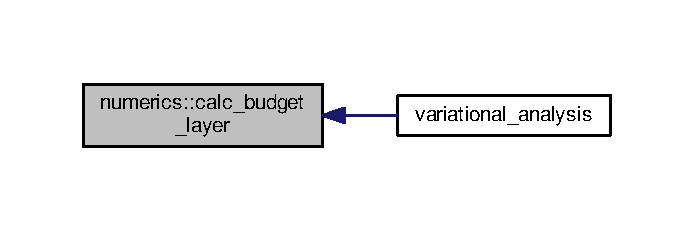
\includegraphics[width=333pt]{namespacenumerics_adbe2d748ef22c981cddde813d1db9d77_icgraph}
\end{center}
\end{figure}


\index{numerics@{numerics}!caldev@{caldev}}
\index{caldev@{caldev}!numerics@{numerics}}
\subsubsection[{\texorpdfstring{caldev(\+D\+U, K\+T, K\+S, N\+S\+T\+U, N\+T\+U, N\+P, N\+V\+U, D\+E\+V\+M2)}{caldev(DU, KT, KS, NSTU, NTU, NP, NVU, DEVM2)}}]{\setlength{\rightskip}{0pt plus 5cm}subroutine numerics\+::caldev (
\begin{DoxyParamCaption}
\item[{real (kind=rk8), dimension(nvu,np,nstu,ntu), intent(in)}]{DU, }
\item[{integer (kind=ik4), intent(in)}]{KT, }
\item[{integer (kind=ik4), intent(in)}]{KS, }
\item[{integer (kind=ik4), intent(in)}]{N\+S\+TU, }
\item[{integer (kind=ik4), intent(in)}]{N\+TU, }
\item[{integer (kind=ik4), intent(in)}]{NP, }
\item[{integer (kind=ik4), intent(in)}]{N\+VU, }
\item[{real (kind=rk8), dimension(nvu,np)}]{D\+E\+V\+M2}
\end{DoxyParamCaption}
)}\hypertarget{namespacenumerics_add44a47f4f996c0266711b825fd6bb20}{}\label{namespacenumerics_add44a47f4f996c0266711b825fd6bb20}


Definition at line 172 of file numerics.\+f90.


\begin{DoxyCode}
172 \textcolor{keywordtype}{USE }\hyperlink{namespaceportable}{portable}
173 \textcolor{keywordtype}{USE }\hyperlink{namespaceconstants}{constants}
174 
175 \textcolor{keywordtype}{INTEGER (KIND=IK4)}, \textcolor{keywordtype}{INTENT(IN)}                          :: kt       \textcolor{comment}{! Top level for the variational
       analysis.}
176 \textcolor{keywordtype}{INTEGER (KIND=IK4)}, \textcolor{keywordtype}{INTENT(IN)}                          :: ks       \textcolor{comment}{! Surface level for the variational
       analysis.}
177 \textcolor{keywordtype}{INTEGER (KIND=IK4)}, \textcolor{keywordtype}{INTENT(IN)}                          :: nstu     \textcolor{comment}{! Number of stations.}
178 \textcolor{keywordtype}{INTEGER (KIND=IK4)}, \textcolor{keywordtype}{INTENT(IN)}                          :: ntu      \textcolor{comment}{! Number of times.}
179 \textcolor{keywordtype}{INTEGER (KIND=IK4)}, \textcolor{keywordtype}{INTENT(IN)}                          :: np       \textcolor{comment}{! Number of pressure levels.}
180 \textcolor{keywordtype}{INTEGER (KIND=IK4)}, \textcolor{keywordtype}{INTENT(IN)}                          :: \hyperlink{namespacesettings_a79e2ff19d589b215ed9176906dd5cbbf}{nvu}      \textcolor{comment}{! Number of variables.}
181 \textcolor{keywordtype}{REAL (KIND=RK8)}, \textcolor{keywordtype}{DIMENSION(NVU,NP,NSTU,NTU)}, \textcolor{keywordtype}{INTENT(IN)} :: du       \textcolor{comment}{! Holds the data (see assim.f90 for a
       description of the array)}
182 \textcolor{keywordtype}{REAL (KIND=RK8)}, \textcolor{keywordtype}{DIMENSION(NVU,NP)}                      :: devm2    \textcolor{comment}{! Holds the RMSE and other stuff.}
183 
184 \textcolor{comment}{!}
185 \textcolor{comment}{! Local variables.}
186 \textcolor{comment}{!}
187 \textcolor{keywordtype}{REAL (KIND=RK8)}, \textcolor{keywordtype}{DIMENSION(NVU,NP)}                      :: devm     \textcolor{comment}{! Holds the time mnd station ean of the
       variables.}
188 \textcolor{keywordtype}{REAL (KIND=RK8)}, \textcolor{keywordtype}{DIMENSION(NVU,NP,NSTU,NTU)}             :: dev      \textcolor{comment}{! The difference between the variables
       and the mean (DEVM)}
189 
190 \textcolor{keywordtype}{INTEGER (KIND=IK4)}                                      :: ii, ist  \textcolor{comment}{!  Counters}
191 
192 \textcolor{comment}{!}
193 \textcolor{comment}{! Here we calculate the mean of the five variables accross the stations at each level. When calculating the
       mean, neglect the}
194 \textcolor{comment}{! start and end times.}
195 \textcolor{comment}{!}
196 devm(2:6,ks:kt) = sum(sum(du(2:6,ks:kt,:,2:ntu-1),dim=4),dim=3)/nstu/(ntu-2)
197 
198 \textcolor{comment}{!}
199 \textcolor{comment}{! Now calculate the difference from the mean. This is easiest to do in a traditional loop.}
200 \textcolor{comment}{!}
201 dev                 = 0.0
202 \textcolor{keywordflow}{DO} ii=2,ntu-1
203     \textcolor{keywordflow}{DO} ist=1,nstu
204         dev(:,:,ist,ii) = du(:,:,ist,ii) - devm(:,:)
205 \textcolor{keywordflow}{    END DO}
206 \textcolor{keywordflow}{END DO}
207 
208 \textcolor{comment}{!}
209 \textcolor{comment}{! Finally, calculate the RMSE.}
210 devm2               = devm
211 devm2(2:6,ks:kt)    = sqrt(sum(sum(dev(2:6,ks:kt,:,2:ntu-1)**2,dim=4),dim=3)/nstu/(ntu-2))
212 
213 devm2(2,:)          = devm2(2,:)/\hyperlink{namespaceconstants_afb3befdfd57058ee9d073b832134a601}{lv0}*\hyperlink{namespaceconstants_a32354adf3493f59d0fc17b0302b2c368}{cpd}    \textcolor{comment}{! The other stuff mentioned above.}
214 
\end{DoxyCode}


Here is the caller graph for this function\+:\nopagebreak
\begin{figure}[H]
\begin{center}
\leavevmode
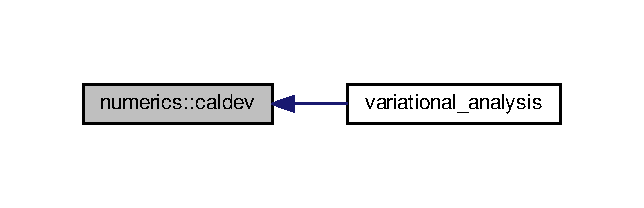
\includegraphics[width=309pt]{namespacenumerics_add44a47f4f996c0266711b825fd6bb20_icgraph}
\end{center}
\end{figure}


\index{numerics@{numerics}!gmean@{gmean}}
\index{gmean@{gmean}!numerics@{numerics}}
\subsubsection[{\texorpdfstring{gmean(\+M\+G, D\+P, N\+V, N\+S\+T, N\+T, T\+S\+M\+O\+O\+T\+H)}{gmean(MG, DP, NV, NST, NT, TSMOOTH)}}]{\setlength{\rightskip}{0pt plus 5cm}subroutine numerics\+::gmean (
\begin{DoxyParamCaption}
\item[{real (kind=rk8), dimension(nt), intent(out)}]{MG, }
\item[{real (kind=rk8), dimension(nv,nst,nt), intent(in)}]{DP, }
\item[{integer (kind=ik4), intent(in)}]{NV, }
\item[{integer (kind=ik4), intent(in)}]{N\+ST, }
\item[{integer (kind=ik4), intent(in)}]{NT, }
\item[{integer (kind=ik4), intent(in)}]{T\+S\+M\+O\+O\+TH}
\end{DoxyParamCaption}
)}\hypertarget{namespacenumerics_afbd04035bb50e63d44980bf39cf84ac3}{}\label{namespacenumerics_afbd04035bb50e63d44980bf39cf84ac3}


Definition at line 61 of file numerics.\+f90.


\begin{DoxyCode}
61 \textcolor{keywordtype}{USE }\hyperlink{namespaceportable}{portable}
62 
63 \textcolor{keywordtype}{IMPLICIT NONE}
64 \textcolor{keywordtype}{INTEGER (KIND=IK4)}, \textcolor{keywordtype}{INTENT(IN)}                      :: nt           \textcolor{comment}{! Number of time steps.}
65 \textcolor{keywordtype}{INTEGER (KIND=IK4)}, \textcolor{keywordtype}{INTENT(IN)}                      :: tsmooth      \textcolor{comment}{! 0 = no smoothing.}
66 \textcolor{keywordtype}{INTEGER (KIND=IK4)}, \textcolor{keywordtype}{INTENT(IN)}                      :: nv           \textcolor{comment}{! Number of variables (only the last
       variable is averaged).}
67 \textcolor{keywordtype}{INTEGER (KIND=IK4)}, \textcolor{keywordtype}{INTENT(IN)}                      :: nst          \textcolor{comment}{! Number of stations in the analysis
       grid.}
68 \textcolor{keywordtype}{REAL (KIND=RK8)}, \textcolor{keywordtype}{DIMENSION(NT)}, \textcolor{keywordtype}{INTENT(OUT)}         :: mg           \textcolor{comment}{! The spatial average of DP is stored
       in this array.}
69 \textcolor{keywordtype}{REAL (KIND=RK8)}, \textcolor{keywordtype}{DIMENSION(NV,NST,NT)}, \textcolor{keywordtype}{INTENT(IN)}   :: dp           \textcolor{comment}{! Data to be averaged, and possibly
       time smoothed.}
70 
71 mg  = sum(dp(nv,:,:), dim=1)/nst        \textcolor{comment}{! Average the last variable along the station dimension (DIM=1,
       because the rank of the}
72                                         \textcolor{comment}{! array subsection is only two (the variable dimension "collapses"
       when the subsection}
73                                         \textcolor{comment}{! is extracted)).}
74 \textcolor{keywordflow}{IF} (tsmooth .GT. 0) \textcolor{keywordflow}{THEN}
75     \textcolor{keyword}{CALL }smooth(mg, \textcolor{keyword}{SIZE}(mg), tsmooth, .false.)
76 \textcolor{keywordflow}{END IF}
77 
\end{DoxyCode}


Here is the call graph for this function\+:\nopagebreak
\begin{figure}[H]
\begin{center}
\leavevmode
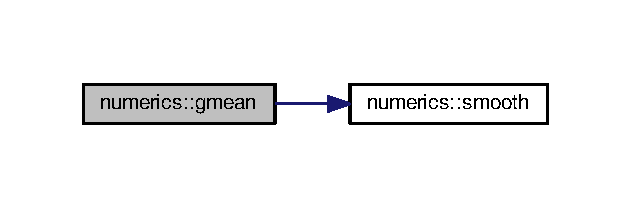
\includegraphics[width=303pt]{namespacenumerics_afbd04035bb50e63d44980bf39cf84ac3_cgraph}
\end{center}
\end{figure}


\index{numerics@{numerics}!horizontal\+\_\+field@{horizontal\+\_\+field}}
\index{horizontal\+\_\+field@{horizontal\+\_\+field}!numerics@{numerics}}
\subsubsection[{\texorpdfstring{horizontal\+\_\+field(\+N\+S\+T, L\+O\+N, L\+A\+T, X, Y, F, D\+Z\+D\+X, D\+Z\+D\+Y, D\+I\+V\+U, D\+I\+V\+V)}{horizontal_field(NST, LON, LAT, X, Y, F, DZDX, DZDY, DIVU, DIVV)}}]{\setlength{\rightskip}{0pt plus 5cm}subroutine numerics\+::horizontal\+\_\+field (
\begin{DoxyParamCaption}
\item[{integer (kind=ik4), intent(in)}]{N\+ST, }
\item[{real (kind=rk8), dimension(nst), intent(in)}]{L\+ON, }
\item[{real (kind=rk8), dimension(nst), intent(in)}]{L\+AT, }
\item[{real (kind=rk8), dimension(nst), intent(out)}]{X, }
\item[{real (kind=rk8), dimension(nst), intent(out)}]{Y, }
\item[{real (kind=rk8), dimension(nst), intent(out)}]{F, }
\item[{real (kind=rk8), dimension(nst), intent(out)}]{D\+Z\+DX, }
\item[{real (kind=rk8), dimension(nst), intent(out)}]{D\+Z\+DY, }
\item[{real (kind=rk8), dimension(nst), intent(out)}]{D\+I\+VU, }
\item[{real (kind=rk8), dimension(nst), intent(out)}]{D\+I\+VV}
\end{DoxyParamCaption}
)}\hypertarget{namespacenumerics_a9581a41d0b81a5ded9690972e499c629}{}\label{namespacenumerics_a9581a41d0b81a5ded9690972e499c629}


Definition at line 231 of file numerics.\+f90.


\begin{DoxyCode}
231 \textcolor{keywordtype}{USE }\hyperlink{namespaceconstants}{constants}
232 
233 \textcolor{keywordtype}{IMPLICIT NONE}
234 \textcolor{keywordtype}{INTEGER (KIND=IK4)}, \textcolor{keywordtype}{INTENT(IN)}                :: nst          \textcolor{comment}{! The number of stations in the array.}
235 \textcolor{keywordtype}{REAL (KIND=RK8)}, \textcolor{keywordtype}{DIMENSION(NST)}, \textcolor{keywordtype}{INTENT(IN)}   :: lon          \textcolor{comment}{! The longitudes of each station.}
236 \textcolor{keywordtype}{REAL (KIND=RK8)}, \textcolor{keywordtype}{DIMENSION(NST)}, \textcolor{keywordtype}{INTENT(IN)}   :: lat          \textcolor{comment}{! The latitudes of each station.}
237 \textcolor{keywordtype}{REAL (KIND=RK8)}, \textcolor{keywordtype}{DIMENSION(NST)}, \textcolor{keywordtype}{INTENT(OUT)}  :: x            \textcolor{comment}{! The cartesian x-coordinates of each
       station.}
238 \textcolor{keywordtype}{REAL (KIND=RK8)}, \textcolor{keywordtype}{DIMENSION(NST)}, \textcolor{keywordtype}{INTENT(OUT)}  :: y            \textcolor{comment}{! The cartesian y-coordinates of each
       station.}
239 \textcolor{keywordtype}{REAL (KIND=RK8)}, \textcolor{keywordtype}{DIMENSION(NST)}, \textcolor{keywordtype}{INTENT(OUT)}  :: f            \textcolor{comment}{! Coriolis parameter at each station.}
240 \textcolor{keywordtype}{REAL (KIND=RK8)}, \textcolor{keywordtype}{DIMENSION(NST)}, \textcolor{keywordtype}{INTENT(OUT)}  :: dzdx         \textcolor{comment}{!}
241 \textcolor{keywordtype}{REAL (KIND=RK8)}, \textcolor{keywordtype}{DIMENSION(NST)}, \textcolor{keywordtype}{INTENT(OUT)}  :: dzdy         \textcolor{comment}{!}
242 \textcolor{keywordtype}{REAL (KIND=RK8)}, \textcolor{keywordtype}{DIMENSION(NST)}, \textcolor{keywordtype}{INTENT(OUT)}  :: divu         \textcolor{comment}{!}
243 \textcolor{keywordtype}{REAL (KIND=RK8)}, \textcolor{keywordtype}{DIMENSION(NST)}, \textcolor{keywordtype}{INTENT(OUT)}  :: divv         \textcolor{comment}{!}
244 
245 \textcolor{comment}{!}
246 \textcolor{comment}{! Local variables.}
247 \textcolor{comment}{!}
248 \textcolor{keywordtype}{REAL (KIND=RK8)}, \textcolor{keywordtype}{DIMENSION(NST)}               :: z1
249 \textcolor{keywordtype}{REAL (KIND=RK8)}, \textcolor{keywordtype}{DIMENSION(NST+2)}             :: x1, y1               \textcolor{comment}{! Holds coordinates of next station
       in the "loop".}
250 \textcolor{keywordtype}{INTEGER (KIND=IK4)}                            :: ii                   \textcolor{comment}{! Counter.}
251 \textcolor{keywordtype}{REAL (KIND=RK8)}                               :: ax, ay, bx, by, c3   \textcolor{comment}{! Temporary variables.}
252 \textcolor{keywordtype}{REAL (KIND=RK8)}                               :: area                 \textcolor{comment}{! Area of sounding array.}
253 
254 \textcolor{comment}{!}
255 \textcolor{comment}{! Calculate the cartesian co-ordinates of each station, and the coriolis parameter at each station.}
256 \textcolor{comment}{!}
257 
258 x   = 2.0*sin((lon-lon(1))/360.0*2*\hyperlink{namespaceconstants_a064bd715409f723a4e6d45b6300c5ca0}{pi}/2.0)*\hyperlink{namespaceconstants_afaa5eaa2c9ee648a808fb8e1c94e76f8}{rearth}*cos(lat/180.0*\hyperlink{namespaceconstants_a064bd715409f723a4e6d45b6300c5ca0}{pi})
259 y   = 2.0*sin((lat-lat(1))/360.0*2*\hyperlink{namespaceconstants_a064bd715409f723a4e6d45b6300c5ca0}{pi}/2.0)*\hyperlink{namespaceconstants_afaa5eaa2c9ee648a808fb8e1c94e76f8}{rearth}
260 f   = 2.0*\hyperlink{namespaceconstants_a67051296d7b4bcd0d4cee08bba6e46fa}{omega}*sin(lat/180.0*\hyperlink{namespaceconstants_a064bd715409f723a4e6d45b6300c5ca0}{pi})
261 
262 \textcolor{comment}{!}
263 \textcolor{comment}{! Calculate the gradient terms. We do this by fitting a plane of best fit to the points.}
264 \textcolor{comment}{!}
265 z1  = 0
266 \textcolor{keywordflow}{DO} ii=1,nst
267     z1(ii)   = 1.0
268     \textcolor{keyword}{CALL }line\_fit\_xyz(nst, x, y, z1, dzdx(ii), dzdy(ii), c3)
269     z1(ii)   = 0.0
270 \textcolor{keywordflow}{END DO}
271 
272 \textcolor{comment}{!}
273 \textcolor{comment}{! Set X1 and Y1 to contain the coordinates of the next station in the "loop"}
274 \textcolor{comment}{!}
275 \textcolor{keywordflow}{DO} ii=1,nst
276     x1(ii+1)    = x(ii)
277     y1(ii+1)    = y(ii)
278 \textcolor{keywordflow}{END DO}
279 x1(1)       = x1(nst+1)
280 y1(1)       = y1(nst+1)
281 x1(nst+2)   = x1(2)
282 y1(nst+2)   = y1(2)
283 
284 \textcolor{comment}{!}
285 \textcolor{comment}{! Calculate the area of the sounding array.}
286 \textcolor{comment}{!}
287 area        = 0.0
288 \textcolor{keywordflow}{DO} ii=2,nst-1
289     ax      = x(1) - x(ii)
290     ay      = y(1) - y(ii)
291     bx      = x(1) - x(ii+1)
292     by      = y(1) - y(ii+1)
293     area    = area + abs(ax*by - ay*bx)/2.0
294 \textcolor{keywordflow}{END DO}
295 
296 \textcolor{comment}{!}
297 \textcolor{comment}{! Now calculate the divergence terms using the line integral method (see Davies-Jones (1993) equations
       8-10)}
298 \textcolor{comment}{!}
299 \textcolor{keywordflow}{DO} ii=1,nst
300     divu(ii)    = (y1(ii+2) - y1(ii))/2.0/area
301     divv(ii)    = -(x1(ii+2) - x1(ii))/2.0/area
302 \textcolor{keywordflow}{END DO}
303 
\end{DoxyCode}


Here is the call graph for this function\+:\nopagebreak
\begin{figure}[H]
\begin{center}
\leavevmode
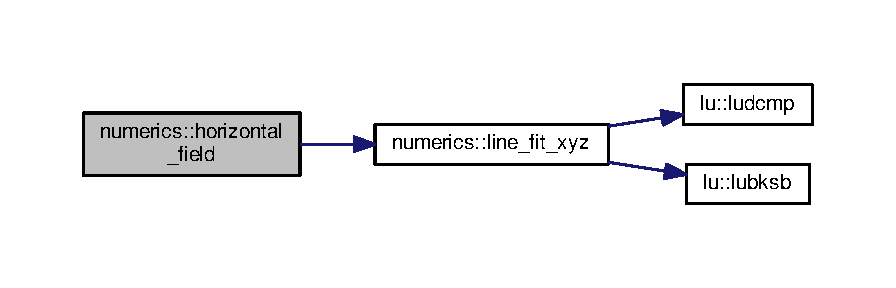
\includegraphics[width=350pt]{namespacenumerics_a9581a41d0b81a5ded9690972e499c629_cgraph}
\end{center}
\end{figure}




Here is the caller graph for this function\+:\nopagebreak
\begin{figure}[H]
\begin{center}
\leavevmode
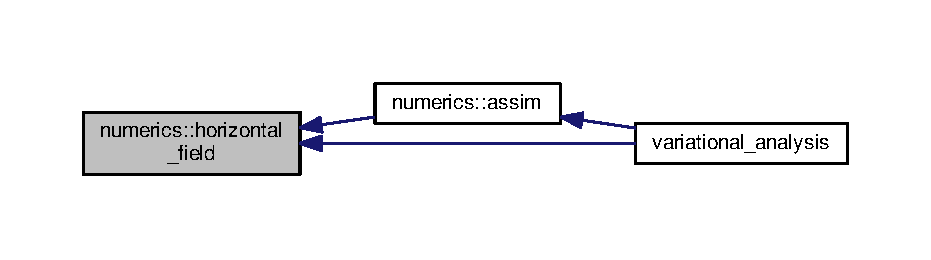
\includegraphics[width=350pt]{namespacenumerics_a9581a41d0b81a5ded9690972e499c629_icgraph}
\end{center}
\end{figure}


\index{numerics@{numerics}!itps@{itps}}
\index{itps@{itps}!numerics@{numerics}}
\subsubsection[{\texorpdfstring{itps(\+K\+S, K\+B, D, D\+S)}{itps(KS, KB, D, DS)}}]{\setlength{\rightskip}{0pt plus 5cm}subroutine numerics\+::itps (
\begin{DoxyParamCaption}
\item[{integer (kind=ik4), intent(in)}]{KS, }
\item[{integer (kind=ik4), intent(in)}]{KB, }
\item[{real (kind=rk8), dimension(\+:), intent(inout)}]{D, }
\item[{real (kind=rk8), intent(in)}]{DS}
\end{DoxyParamCaption}
)}\hypertarget{namespacenumerics_ac972e0e69239cba641ad373fee101472}{}\label{namespacenumerics_ac972e0e69239cba641ad373fee101472}


Definition at line 23 of file numerics.\+f90.


\begin{DoxyCode}
23 \textcolor{keywordtype}{USE }\hyperlink{namespaceportable}{portable}
24 
25 \textcolor{keywordtype}{IMPLICIT NONE}
26 
27 \textcolor{keywordtype}{INTEGER (KIND=IK4)}, \textcolor{keywordtype}{INTENT(IN)}              :: ks   \textcolor{comment}{! Level where the surface pressure is.}
28 \textcolor{keywordtype}{INTEGER (KIND=IK4)}, \textcolor{keywordtype}{INTENT(IN)}              :: kb   \textcolor{comment}{! Level where the actual surface is.}
29 \textcolor{keywordtype}{REAL (KIND=RK8)}, \textcolor{keywordtype}{DIMENSION(:)},\textcolor{keywordtype}{INTENT(INOUT)} :: d    \textcolor{comment}{! Array to hold interpolated data.}
30 \textcolor{keywordtype}{REAL (KIND=RK8)}, \textcolor{keywordtype}{INTENT(IN)}                 :: ds   \textcolor{comment}{! Value of D at the level where the surface pressure
       is.}
31 
32 \textcolor{comment}{!}
33 \textcolor{comment}{! Local variables.}
34 \textcolor{comment}{!}
35 \textcolor{keywordtype}{INTEGER (KIND=IK4)}                          :: kk   \textcolor{comment}{! Counter.}
36 
37 \textcolor{keywordflow}{IF} (ks .LT. kb) \textcolor{keywordflow}{THEN}
38     \textcolor{comment}{!}
39     \textcolor{comment}{! If we enter this loop, the surface pressure level is lower than the level where the surface is. No
       other case}
40     \textcolor{comment}{! (apart from the ideal one, where the surface pressure and surface levels are the same) is considered.}
41     \textcolor{comment}{!}
42     d(ks)       = ds
43     \textcolor{keywordflow}{DO} kk=ks+1,kb-1
44         d(kk)   = ds + (d(kb) - ds)/(kb - ks)*(kk - ks)
45 \textcolor{keywordflow}{    END DO}
46 \textcolor{keywordflow}{END IF}
47 
\end{DoxyCode}


Here is the caller graph for this function\+:\nopagebreak
\begin{figure}[H]
\begin{center}
\leavevmode
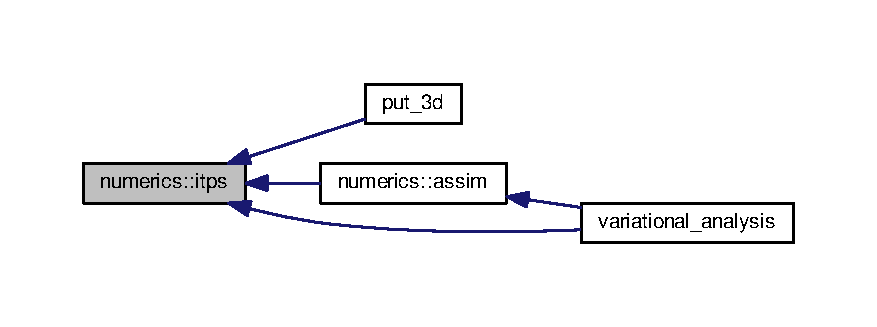
\includegraphics[width=350pt]{namespacenumerics_ac972e0e69239cba641ad373fee101472_icgraph}
\end{center}
\end{figure}


\index{numerics@{numerics}!line\+\_\+fit\+\_\+xyz@{line\+\_\+fit\+\_\+xyz}}
\index{line\+\_\+fit\+\_\+xyz@{line\+\_\+fit\+\_\+xyz}!numerics@{numerics}}
\subsubsection[{\texorpdfstring{line\+\_\+fit\+\_\+xyz(\+N, X, Y, Z, D\+Z\+D\+X, D\+Z\+D\+Y, Z0)}{line_fit_xyz(N, X, Y, Z, DZDX, DZDY, Z0)}}]{\setlength{\rightskip}{0pt plus 5cm}subroutine numerics\+::line\+\_\+fit\+\_\+xyz (
\begin{DoxyParamCaption}
\item[{integer (kind=ik4), intent(in)}]{N, }
\item[{real (kind=rk8), dimension(n), intent(in)}]{X, }
\item[{real (kind=rk8), dimension(n), intent(in)}]{Y, }
\item[{real (kind=rk8), dimension(n), intent(in)}]{Z, }
\item[{real (kind=rk8), intent(out)}]{D\+Z\+DX, }
\item[{real (kind=rk8), intent(out)}]{D\+Z\+DY, }
\item[{real (kind=rk8), intent(out)}]{Z0}
\end{DoxyParamCaption}
)}\hypertarget{namespacenumerics_a8e58d8bf1c738af1a91517fdb8b81aa2}{}\label{namespacenumerics_a8e58d8bf1c738af1a91517fdb8b81aa2}


Definition at line 318 of file numerics.\+f90.


\begin{DoxyCode}
318 \textcolor{keywordtype}{USE }\hyperlink{namespaceportable}{portable}
319 \textcolor{keywordtype}{USE }\hyperlink{namespacelu}{lu}
320 
321 \textcolor{keywordtype}{IMPLICIT NONE}
322 
323 \textcolor{keywordtype}{INTEGER (KIND=IK4)}, \textcolor{keywordtype}{INTENT(IN)}              :: n            \textcolor{comment}{! The number of points}
324 \textcolor{keywordtype}{REAL (KIND=RK8)}, \textcolor{keywordtype}{DIMENSION(N)}, \textcolor{keywordtype}{INTENT(IN)}   :: x            \textcolor{comment}{! The cartesian x-coordinates of each point}
325 \textcolor{keywordtype}{REAL (KIND=RK8)}, \textcolor{keywordtype}{DIMENSION(N)}, \textcolor{keywordtype}{INTENT(IN)}   :: y            \textcolor{comment}{! The cartesian y-coordinates of each point}
326 \textcolor{keywordtype}{REAL (KIND=RK8)}, \textcolor{keywordtype}{DIMENSION(N)}, \textcolor{keywordtype}{INTENT(IN)}   :: z            \textcolor{comment}{! The z-value at each point}
327 \textcolor{keywordtype}{REAL (KIND=RK8)}, \textcolor{keywordtype}{INTENT(OUT)}                :: dzdx         \textcolor{comment}{! Slope of the plane in the x-direction}
328 \textcolor{keywordtype}{REAL (KIND=RK8)}, \textcolor{keywordtype}{INTENT(OUT)}                :: dzdy         \textcolor{comment}{! Slope of the plane in the y-direction}
329 \textcolor{keywordtype}{REAL (KIND=RK8)}, \textcolor{keywordtype}{INTENT(OUT)}                :: z0           \textcolor{comment}{! z-value at (x,y) = (0,0)}
330 
331 \textcolor{comment}{!}
332 \textcolor{comment}{! Local variables.}
333 \textcolor{comment}{!}
334 \textcolor{keywordtype}{REAL (KIND=RK8)}, \textcolor{keywordtype}{DIMENSION(3,3)}             :: a 
335 \textcolor{keywordtype}{REAL (KIND=RK8)}, \textcolor{keywordtype}{DIMENSION(3)}               :: b
336 \textcolor{keywordtype}{INTEGER (KIND=IK4)}, \textcolor{keywordtype}{DIMENSION(3)}            :: indx
337 \textcolor{keywordtype}{INTEGER (KIND=IK4)}                          :: code, d
338 
339 \textcolor{comment}{!}
340 \textcolor{comment}{! By solving the equation    | sum(x^2)  sum(xy)     sum(x)  |     | sum(xz) |}
341 \textcolor{comment}{!                            | sum(xy)   sum(y^2)    sum(y)  | X = | sum(yz) |}
342 \textcolor{comment}{!                            | sum(x)    sum(y)      N       |     | sum(z)  |}
343 \textcolor{comment}{!}
344 \textcolor{comment}{! for X, we can find the slopes DZDX, DZDY aand the intercept Z0 (all defined above) for the plane of best
       fit:}
345 \textcolor{comment}{!}
346 \textcolor{comment}{!     | DZDX |}
347 \textcolor{comment}{! X = | DZDY |}
348 \textcolor{comment}{!     |  Z0  |}
349 \textcolor{comment}{!}
350 \textcolor{comment}{! Whoever worked this out was pretty clever.}
351 \textcolor{comment}{!}
352 
353 a = reshape(source=(/   sum(x*x), sum(x*y), sum(x), &
354 &                       sum(x*y), sum(y*y), sum(y), &
355 &                       sum(x),   sum(y),   \textcolor{keywordtype}{REAL(N, RK8)} /), shape=(/ 3, 3 /))
356 
357 b = (/ sum(x*z), sum(y*z), sum(z) /)
358 
359 \textcolor{comment}{!}
360 \textcolor{comment}{! These calls solve the matrix equation AX=B. First, we calculate the LU decomposition of A using the
       LUDCMP}
361 \textcolor{comment}{! subroutine, then we solve for X using the LUBKSB subroutine. Details on the maths behind all this can be
       found}
362 \textcolor{comment}{! from many sources.}
363 \textcolor{comment}{!}
364 \textcolor{keyword}{CALL }\hyperlink{namespacelu_a578a2275703e9c18d7f262f0a3482fbe}{ludcmp}(a, 3, indx, d, code)
365 \textcolor{keywordflow}{IF} (code .EQ. 1) \textcolor{keywordflow}{THEN}
366     print *,\textcolor{stringliteral}{'W: Tried to do a LU decomposition on a singular matrix.'}
367     print *,\textcolor{stringliteral}{'   This code is not clever enough to handle this case.'}
368     stop \textcolor{stringliteral}{'1'}
369 \textcolor{keywordflow}{END IF}
370 \textcolor{keyword}{CALL }\hyperlink{namespacelu_a588ba20d76e8dd5c49b370d9ba3ec379}{lubksb}(a, 3, indx, b)
371 
372 dzdx = b(1)
373 dzdy = b(2)
374 z0   = b(3)
375 
\end{DoxyCode}


Here is the call graph for this function\+:\nopagebreak
\begin{figure}[H]
\begin{center}
\leavevmode
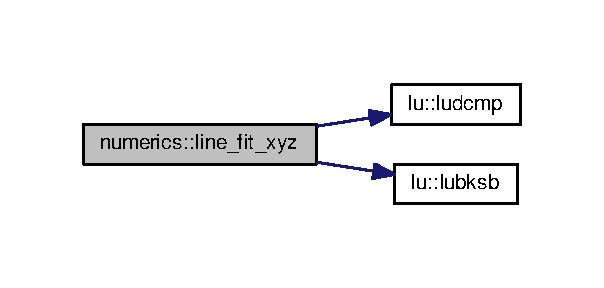
\includegraphics[width=290pt]{namespacenumerics_a8e58d8bf1c738af1a91517fdb8b81aa2_cgraph}
\end{center}
\end{figure}




Here is the caller graph for this function\+:\nopagebreak
\begin{figure}[H]
\begin{center}
\leavevmode
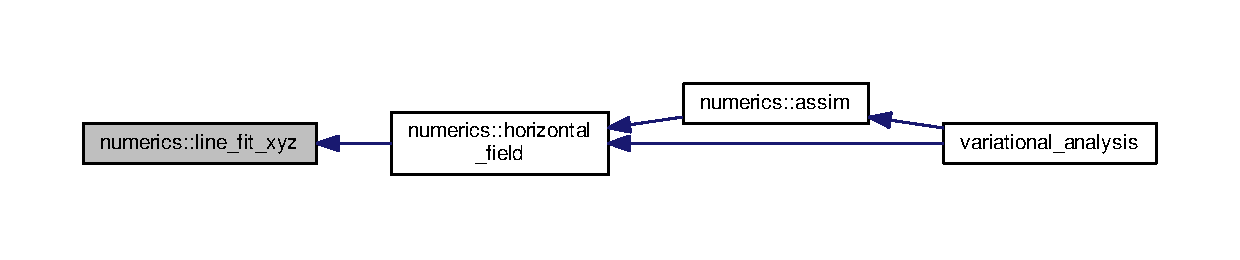
\includegraphics[width=350pt]{namespacenumerics_a8e58d8bf1c738af1a91517fdb8b81aa2_icgraph}
\end{center}
\end{figure}


\index{numerics@{numerics}!smooth@{smooth}}
\index{smooth@{smooth}!numerics@{numerics}}
\subsubsection[{\texorpdfstring{smooth(\+A\+R\+R\+A\+Y, N, F\+I\+L\+T\+E\+R\+\_\+\+W\+I\+D\+T\+H, C\+Y\+C\+L\+I\+C)}{smooth(ARRAY, N, FILTER_WIDTH, CYCLIC)}}]{\setlength{\rightskip}{0pt plus 5cm}subroutine numerics\+::smooth (
\begin{DoxyParamCaption}
\item[{real (kind=rk8), dimension(n), intent(inout)}]{A\+R\+R\+AY, }
\item[{integer (kind=ik4), intent(in)}]{N, }
\item[{integer (kind=ik4), intent(in)}]{F\+I\+L\+T\+E\+R\+\_\+\+W\+I\+D\+TH, }
\item[{logical, intent(in)}]{C\+Y\+C\+L\+IC}
\end{DoxyParamCaption}
)}\hypertarget{namespacenumerics_a354d8c793bd1515de7af7cfa32c51389}{}\label{namespacenumerics_a354d8c793bd1515de7af7cfa32c51389}


Definition at line 90 of file numerics.\+f90.


\begin{DoxyCode}
90 \textcolor{keywordtype}{USE }\hyperlink{namespaceportable}{portable}
91 
92 \textcolor{keywordtype}{IMPLICIT NONE}
93 \textcolor{keywordtype}{INTEGER (KIND=IK4)}, \textcolor{keywordtype}{INTENT(IN)}                      :: n            \textcolor{comment}{! Number of elements in ARRAY.}
94 \textcolor{keywordtype}{INTEGER (KIND=IK4)}, \textcolor{keywordtype}{INTENT(IN)}                      :: filter\_width \textcolor{comment}{! Width of the box car filter.}
95 \textcolor{keywordtype}{REAL (KIND=RK8)}, \textcolor{keywordtype}{DIMENSION(N)}, \textcolor{keywordtype}{INTENT(INOUT)}        :: array        \textcolor{comment}{! The array of data being filtered.}
96 \textcolor{keywordtype}{LOGICAL}, \textcolor{keywordtype}{INTENT(IN)}                                 :: cyclic       \textcolor{comment}{! Set to .TRUE. if data are cyclic.}
97 
98 \textcolor{comment}{!}
99 \textcolor{comment}{! Local variables.}
100 \textcolor{comment}{!}
101 \textcolor{keywordtype}{REAL (KIND=RK8)}, \textcolor{keywordtype}{DIMENSION(:)}, \textcolor{keywordtype}{ALLOCATABLE}          :: tmparray1,tmparray2     \textcolor{comment}{! Temporary array used for
       filtering.}
102 \textcolor{keywordtype}{INTEGER (KIND=IK4)}                                  :: tmpwidth     \textcolor{comment}{! Filter width.}
103 \textcolor{keywordtype}{INTEGER (KIND=IK4)}                                  :: memst        \textcolor{comment}{! Status code from memory allocation
       functions.}
104 \textcolor{keywordtype}{INTEGER (KIND=IK4)}                                  :: ii           \textcolor{comment}{! Counter.}
105 
106 \textcolor{comment}{!}
107 \textcolor{comment}{! First check that (i) the filter width is not too large, and (ii) the filter width is an odd number. If
       the filter width is an even}
108 \textcolor{comment}{! number, we set a temporary filter width which is one greater than the value passed to the subroutine.}
109 \textcolor{comment}{!}
110 \textcolor{keywordflow}{IF} (mod(filter\_width, 2) .EQ. 0) \textcolor{keywordflow}{THEN}
111     tmpwidth    = filter\_width + 1
112 \textcolor{keywordflow}{ELSE}
113     tmpwidth    = filter\_width
114 \textcolor{keywordflow}{END IF}
115 
116 \textcolor{keywordflow}{IF} (tmpwidth .GT. n) \textcolor{keywordflow}{THEN}
117     print *,\textcolor{stringliteral}{'W: Setting filter width to be the same as the number of points in array, '},n
118     tmpwidth    = n
119 \textcolor{keywordflow}{END IF}
120 
121 
122 \textcolor{comment}{!}
123 \textcolor{comment}{! Allocate a temporary array to be used with filtering. If the data are cyclic, then this array is slightly
       larger, to allow}
124 \textcolor{comment}{! us to nicely handle data at the beginning and ends of the array.}
125 \textcolor{comment}{!}
126 \textcolor{keywordflow}{IF} (cyclic) \textcolor{keywordflow}{THEN}
127     \textcolor{keyword}{ALLOCATE}(tmparray1(n+tmpwidth-1), tmparray2(n+tmpwidth-1), stat=memst)
128     \textcolor{keywordflow}{IF} (memst .NE. 0) \textcolor{keywordflow}{THEN}
129         print *,\textcolor{stringliteral}{'Not able to allocate memory for the temporary filtering array'}
130         stop \textcolor{stringliteral}{'1'}
131 \textcolor{keywordflow}{    END IF}
132     tmparray1(1:tmpwidth/2)                  = array(n-tmpwidth/2+1:n)   \textcolor{comment}{! I think this still works when
       TMPWIDTH/2 = 0}
133     tmparray1(tmpwidth/2+1:tmpwidth/2+n)     = array(1:n)
134     tmparray1(tmpwidth/2+n+1:tmpwidth+n-1)   = array(1:tmpwidth/2)
135 \textcolor{keywordflow}{ELSE}
136     \textcolor{keyword}{ALLOCATE}(tmparray1(n), tmparray2(n), stat=memst)
137     \textcolor{keywordflow}{IF} (memst .NE. 0) \textcolor{keywordflow}{THEN}
138         print *,\textcolor{stringliteral}{'Not able to allocate memory for the temporary filtering array'}
139         stop \textcolor{stringliteral}{'1'}
140 \textcolor{keywordflow}{    END IF}
141     tmparray1    = array
142 \textcolor{keywordflow}{END IF}
143 
144 \textcolor{comment}{!}
145 \textcolor{comment}{! Now do the box car filtering.}
146 \textcolor{comment}{!}
147 \textcolor{keywordflow}{DO} ii=1,\textcolor{keyword}{SIZE}(tmparray2)
148         tmparray2(ii)   = sum(tmparray1(max(1, ii-tmpwidth/2):min(ii+tmpwidth/2, \textcolor{keyword}{SIZE}(tmparray2))))/
      tmpwidth
149 \textcolor{keywordflow}{END DO}
150 
151 array(1:n)  = tmparray2(tmpwidth/2+1:tmpwidth/2+n)
152 
153 \textcolor{comment}{!}
154 \textcolor{comment}{! Deallocate allocated memory.}
155 \textcolor{comment}{!}
156 \textcolor{keywordflow}{IF} (\textcolor{keyword}{ALLOCATED}(tmparray1))    \textcolor{keyword}{DEALLOCATE}(tmparray1)
157 \textcolor{keywordflow}{IF} (\textcolor{keyword}{ALLOCATED}(tmparray2))    \textcolor{keyword}{DEALLOCATE}(tmparray2)
158 
\end{DoxyCode}


Here is the caller graph for this function\+:\nopagebreak
\begin{figure}[H]
\begin{center}
\leavevmode
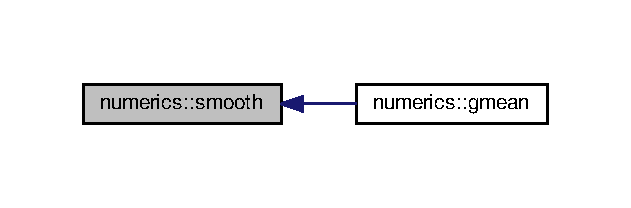
\includegraphics[width=303pt]{namespacenumerics_a354d8c793bd1515de7af7cfa32c51389_icgraph}
\end{center}
\end{figure}


\index{numerics@{numerics}!windown@{windown}}
\index{windown@{windown}!numerics@{numerics}}
\subsubsection[{\texorpdfstring{windown(\+N, X, D\+X, X1, L0, L1)}{windown(N, X, DX, X1, L0, L1)}}]{\setlength{\rightskip}{0pt plus 5cm}subroutine numerics\+::windown (
\begin{DoxyParamCaption}
\item[{integer (kind=ik4), intent(in)}]{N, }
\item[{real (kind=rk8), dimension(n), intent(in)}]{X, }
\item[{real(kind=rk8), intent(in)}]{DX, }
\item[{real (kind=rk8), intent(in)}]{X1, }
\item[{integer (kind=ik4), intent(in)}]{L0, }
\item[{integer (kind=ik4), intent(out)}]{L1}
\end{DoxyParamCaption}
)}\hypertarget{namespacenumerics_aa16b459eac85058fd1da1b9ebc4555b9}{}\label{namespacenumerics_aa16b459eac85058fd1da1b9ebc4555b9}


Definition at line 389 of file numerics.\+f90.


\begin{DoxyCode}
389 \textcolor{keywordtype}{USE }\hyperlink{namespaceportable}{portable}
390 
391 \textcolor{keywordtype}{IMPLICIT NONE}
392 \textcolor{keywordtype}{INTEGER (KIND=IK4)}, \textcolor{keywordtype}{INTENT(IN)}                  :: n        \textcolor{comment}{! Number of vertical layers.}
393 \textcolor{keywordtype}{REAL (KIND=RK8)}, \textcolor{keywordtype}{DIMENSION(N)}, \textcolor{keywordtype}{INTENT(IN)}       :: x        \textcolor{comment}{! Array containing the levels of each layer.}
394 \textcolor{keywordtype}{REAL(KIND=RK8)}, \textcolor{keywordtype}{INTENT(IN)}                      :: dx       \textcolor{comment}{! Layer depth (assume layers are equal depth).}
395 \textcolor{keywordtype}{REAL (KIND=RK8)}, \textcolor{keywordtype}{INTENT(IN)}                     :: x1       \textcolor{comment}{! We are searching for the layer which includes
       this level.}
396 \textcolor{keywordtype}{INTEGER (KIND=IK4)}, \textcolor{keywordtype}{INTENT(IN)}                  :: l0       \textcolor{comment}{! The bottom layer to start searching at.}
397 \textcolor{keywordtype}{INTEGER (KIND=IK4)}, \textcolor{keywordtype}{INTENT(OUT)}                 :: l1       \textcolor{comment}{! The index of the layer which contains the X1
       level.}
398 
399 \textcolor{comment}{!}
400 \textcolor{comment}{! Local variables.}
401 \textcolor{comment}{!}
402 \textcolor{keywordtype}{REAL (KIND=RK8)}                                 :: xa, xb   \textcolor{comment}{! Top and bottom of the vertical layer.}
403 \textcolor{keywordtype}{INTEGER (KIND=IK4)}                              :: ll       \textcolor{comment}{! Layer number.}
404 
405 l1      = -1
406 ll      = l0
407 \textcolor{keywordflow}{DO} \textcolor{keywordflow}{WHILE} ((ll .LE. n) .AND. (l1 .EQ. -1))
408     xa  = x(ll) - dx*(0.5+0.1)
409     xb  = x(ll) + dx*(0.5-0.1)
410     \textcolor{keywordflow}{IF} ((x1 .GE. xa) .AND. (x1 .LT. xb)) l1 = ll
411     ll  = ll + 1
412 \textcolor{keywordflow}{END DO}
413 
\end{DoxyCode}


Here is the caller graph for this function\+:\nopagebreak
\begin{figure}[H]
\begin{center}
\leavevmode
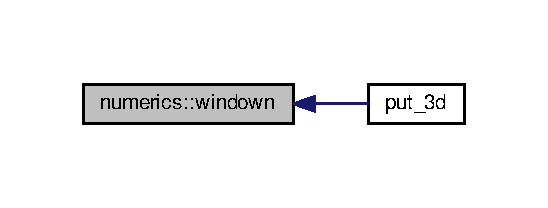
\includegraphics[width=263pt]{namespacenumerics_aa16b459eac85058fd1da1b9ebc4555b9_icgraph}
\end{center}
\end{figure}



\hypertarget{namespacephysics}{}\section{physics Module Reference}
\label{namespacephysics}\index{physics@{physics}}
\subsection*{Functions/\+Subroutines}
\begin{DoxyCompactItemize}
\item 
subroutine \hyperlink{namespacephysics_a3f1959e7b3ff1a8d052f1e0441b1c379}{s\+\_\+r\+\_\+to\+\_\+t\+\_\+z} (P, PS, ZS, S, R, T, Z)
\item 
subroutine \hyperlink{namespacephysics_aebc42cd426e3ef8e85696bb1c7da18c3}{t\+\_\+r\+\_\+to\+\_\+s\+\_\+z} (P, PS, ZS, T, R, S, Z)
\item 
subroutine \hyperlink{namespacephysics_adc35216d512f6586071a79fba286a39c}{diverg} (U\+N\+I\+TH, V\+AR, U, V, D\+I\+VU, D\+I\+VV, D\+I\+V1)
\item 
subroutine \hyperlink{namespacephysics_a56a179b5bd2c13a2201b2367037a42cf}{fcorlx} (U\+N\+I\+TH, N\+S\+TU, F, V, F\+C\+X1)
\item 
subroutine \hyperlink{namespacephysics_a1f64bd544ea55c7fbbf5330725fc0896}{fcorly} (U\+N\+I\+TH, N\+S\+TU, F, U, F\+C\+Y1)
\item 
subroutine \hyperlink{namespacephysics_acf841366af6f4fd7502b4031a2cacb56}{fpgd} (U\+N\+I\+TH, Z, D\+Z\+DX, F\+P1)
\item 
subroutine \hyperlink{namespacephysics_a0ca41ce81224f2d7b292dc474c080c60}{height} (NP, KS, KT, P, T, R, Z)
\item 
subroutine \hyperlink{namespacephysics_a16ab28545ccd5528dd72f50208761dbe}{calht2} (PS, ZS, N, P, TC, R, HT, D\+EW)
\item 
subroutine \hyperlink{namespacephysics_a9197b79c7b8e6dfce5ecca360c320610}{calc\+\_\+state2} (P, T, TD, E, Z, R, RH, H, H\+D\+RY, S)
\end{DoxyCompactItemize}


\subsection{Function/\+Subroutine Documentation}
\index{physics@{physics}!calc\+\_\+state2@{calc\+\_\+state2}}
\index{calc\+\_\+state2@{calc\+\_\+state2}!physics@{physics}}
\subsubsection[{\texorpdfstring{calc\+\_\+state2(\+P, T, T\+D, E, Z, R, R\+H, H, H\+D\+R\+Y, S)}{calc_state2(P, T, TD, E, Z, R, RH, H, HDRY, S)}}]{\setlength{\rightskip}{0pt plus 5cm}subroutine physics\+::calc\+\_\+state2 (
\begin{DoxyParamCaption}
\item[{real (kind=rk8), intent(in)}]{P, }
\item[{real (kind=rk8), intent(in)}]{T, }
\item[{real (kind=rk8), intent(in)}]{TD, }
\item[{real (kind=rk8), intent(in)}]{E, }
\item[{real (kind=rk8), intent(in)}]{Z, }
\item[{real (kind=rk8), intent(out)}]{R, }
\item[{real (kind=rk8), intent(in)}]{RH, }
\item[{real (kind=rk8), intent(out)}]{H, }
\item[{real (kind=rk8), intent(out)}]{H\+D\+RY, }
\item[{real (kind=rk8), intent(out)}]{S}
\end{DoxyParamCaption}
)}\hypertarget{namespacephysics_a9197b79c7b8e6dfce5ecca360c320610}{}\label{namespacephysics_a9197b79c7b8e6dfce5ecca360c320610}


Definition at line 368 of file physics.\+f90.


\begin{DoxyCode}
368 \textcolor{keywordtype}{USE }\hyperlink{namespaceportable}{portable}
369 \textcolor{keywordtype}{USE }\hyperlink{namespaceconstants}{constants}
370 
371 \textcolor{keywordtype}{IMPLICIT NONE}
372 \textcolor{keywordtype}{REAL (KIND=RK8)}, \textcolor{keywordtype}{INTENT(IN)}     :: p    \textcolor{comment}{! Pressure (Pa) - check units.}
373 \textcolor{keywordtype}{REAL (KIND=RK8)}, \textcolor{keywordtype}{INTENT(IN)}     :: t    \textcolor{comment}{! Temperature (K).}
374 \textcolor{keywordtype}{REAL (KIND=RK8)}, \textcolor{keywordtype}{INTENT(IN)}     :: td   \textcolor{comment}{! Dew point temperature (K).}
375 \textcolor{keywordtype}{REAL (KIND=RK8)}, \textcolor{keywordtype}{INTENT(IN)}     :: e    \textcolor{comment}{! Vapour pressure (Pa - check units.}
376 \textcolor{keywordtype}{REAL (KIND=RK8)}, \textcolor{keywordtype}{INTENT(IN)}     :: z    \textcolor{comment}{! Geopotential height (m) - check units.}
377 \textcolor{keywordtype}{REAL (KIND=RK8)}, \textcolor{keywordtype}{INTENT(OUT)}    :: r    \textcolor{comment}{! Mixing ratio.}
378 \textcolor{keywordtype}{REAL (KIND=RK8)}, \textcolor{keywordtype}{INTENT(IN)}     :: rh   \textcolor{comment}{! Relative humidity (decimal fraction between 0 and 1). }
379 \textcolor{keywordtype}{REAL (KIND=RK8)}, \textcolor{keywordtype}{INTENT(OUT)}    :: h    \textcolor{comment}{!}
380 \textcolor{keywordtype}{REAL (KIND=RK8)}, \textcolor{keywordtype}{INTENT(OUT)}    :: hdry \textcolor{comment}{!}
381 \textcolor{keywordtype}{REAL (KIND=RK8)}, \textcolor{keywordtype}{INTENT(OUT)}    :: s    \textcolor{comment}{!}
382 
383 \textcolor{comment}{!}
384 \textcolor{comment}{! Local variables.}
385 \textcolor{comment}{!}
386 \textcolor{keywordtype}{REAL (KIND=RK8)}                 :: ep, es, rs, lv1
387 
388 ep      = \hyperlink{namespaceconstants_ad91564da82b97ea0d29ce0565565db85}{rd}/\hyperlink{namespaceconstants_a7ef8fc37397fbfbefd3c22883378dcc5}{rw}
389 es      = 1.003*exp(53.67957 - 6743.769/t - 4.8451*log(t))  \textcolor{comment}{! An empirical formula for the saturation
       vapour pressure.}
390 rs      = ep*es/(p-es)
391 r       = rs*rh
392 lv1     = \hyperlink{namespaceconstants_afb3befdfd57058ee9d073b832134a601}{lv0} + (\hyperlink{namespaceconstants_afc5ea9cd5f9cf3a42e750ba5ab73c967}{cpv}-\hyperlink{namespaceconstants_a4f2911e99beba65b9371b9a80d7c08d0}{cl})*(t-\hyperlink{namespaceconstants_a753fbbdd5d5b4af00d6819cb78ba99a1}{t0})
393 h       = (\hyperlink{namespaceconstants_a32354adf3493f59d0fc17b0302b2c368}{cpd} + r*\hyperlink{namespaceconstants_a4f2911e99beba65b9371b9a80d7c08d0}{cl})*t + lv1*r + (1.0 + r)*\hyperlink{namespaceconstants_a046aef138fbc8d05251d4fdc6eb3ee89}{g}*z
394 hdry    = \hyperlink{namespaceconstants_a32354adf3493f59d0fc17b0302b2c368}{cpd}*t + \hyperlink{namespaceconstants_a046aef138fbc8d05251d4fdc6eb3ee89}{g}*z
395 s       = \hyperlink{namespaceconstants_a32354adf3493f59d0fc17b0302b2c368}{cpd}*log(t) - \hyperlink{namespaceconstants_ad91564da82b97ea0d29ce0565565db85}{rd}*log(p) + \hyperlink{namespaceconstants_afb3befdfd57058ee9d073b832134a601}{lv0}*r/t - r*\hyperlink{namespaceconstants_a7ef8fc37397fbfbefd3c22883378dcc5}{rw}*log(rh)
\end{DoxyCode}


Here is the caller graph for this function\+:\nopagebreak
\begin{figure}[H]
\begin{center}
\leavevmode
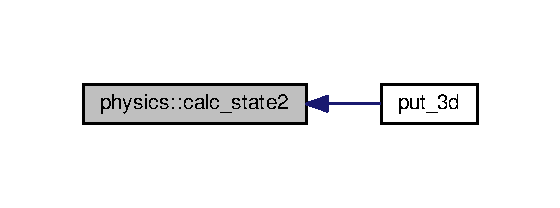
\includegraphics[width=269pt]{namespacephysics_a9197b79c7b8e6dfce5ecca360c320610_icgraph}
\end{center}
\end{figure}


\index{physics@{physics}!calht2@{calht2}}
\index{calht2@{calht2}!physics@{physics}}
\subsubsection[{\texorpdfstring{calht2(\+P\+S, Z\+S, N, P, T\+C, R, H\+T, D\+E\+W)}{calht2(PS, ZS, N, P, TC, R, HT, DEW)}}]{\setlength{\rightskip}{0pt plus 5cm}subroutine physics\+::calht2 (
\begin{DoxyParamCaption}
\item[{real (kind=rk8), intent(in)}]{PS, }
\item[{real (kind=rk8), intent(in)}]{ZS, }
\item[{integer (kind=ik4), intent(in)}]{N, }
\item[{real (kind=rk8), dimension(n), intent(in)}]{P, }
\item[{real (kind=rk8), dimension(n), intent(in)}]{TC, }
\item[{real (kind=rk8), dimension(n), intent(inout)}]{R, }
\item[{real (kind=rk8), dimension(n), intent(out)}]{HT, }
\item[{real (kind=rk8), dimension(n), intent(out)}]{D\+EW}
\end{DoxyParamCaption}
)}\hypertarget{namespacephysics_a16ab28545ccd5528dd72f50208761dbe}{}\label{namespacephysics_a16ab28545ccd5528dd72f50208761dbe}


Definition at line 284 of file physics.\+f90.


\begin{DoxyCode}
284 \textcolor{keywordtype}{USE }\hyperlink{namespaceportable}{portable}
285 \textcolor{keywordtype}{USE }\hyperlink{namespaceconstants}{constants}
286 
287 \textcolor{keywordtype}{IMPLICIT NONE}
288 \textcolor{keywordtype}{REAL (KIND=RK8)}, \textcolor{keywordtype}{INTENT(IN)}                       :: ps     \textcolor{comment}{! Surface pressure (units).}
289 \textcolor{keywordtype}{REAL (KIND=RK8)}, \textcolor{keywordtype}{INTENT(IN)}                       :: zs     \textcolor{comment}{! Surface geopotential (units).}
290 \textcolor{keywordtype}{INTEGER (KIND=IK4)}, \textcolor{keywordtype}{INTENT(IN)}                    :: n      \textcolor{comment}{! Number of vertical levels.}
291 \textcolor{keywordtype}{REAL (KIND=RK8)}, \textcolor{keywordtype}{DIMENSION(N)}, \textcolor{keywordtype}{INTENT(IN)}         :: p      \textcolor{comment}{! Pressures (units).}
292 \textcolor{keywordtype}{REAL (KIND=RK8)}, \textcolor{keywordtype}{DIMENSION(N)}, \textcolor{keywordtype}{INTENT(IN)}         :: tc     \textcolor{comment}{! Temperatures (Celsius).}
293 \textcolor{keywordtype}{REAL (KIND=RK8)}, \textcolor{keywordtype}{DIMENSION(N)}, \textcolor{keywordtype}{INTENT(INOUT)}      :: r      \textcolor{comment}{! Relative humidity (%).}
294 \textcolor{keywordtype}{REAL (KIND=RK8)}, \textcolor{keywordtype}{DIMENSION(N)}, \textcolor{keywordtype}{INTENT(OUT)}        :: ht     \textcolor{comment}{! Geopotential height (units).}
295 \textcolor{keywordtype}{REAL (KIND=RK8)}, \textcolor{keywordtype}{DIMENSION(N)}, \textcolor{keywordtype}{INTENT(OUT)}        :: dew    \textcolor{comment}{! Dew-point temperature? (units).}
296 
297 \textcolor{comment}{!}
298 \textcolor{comment}{! Local variables.}
299 \textcolor{comment}{!}
300 \textcolor{keywordtype}{REAL (KIND=RK8)}, \textcolor{keywordtype}{DIMENSION(N)}                     :: rh     \textcolor{comment}{! Relative humidity converted to 0-1 range.}
301 \textcolor{keywordtype}{REAL (KIND=RK8)}, \textcolor{keywordtype}{DIMENSION(N)}                     :: t      \textcolor{comment}{! Temperature in Kelvin.}
302 \textcolor{keywordtype}{REAL (KIND=RK8)}, \textcolor{keywordtype}{DIMENSION(N)}                     :: es     \textcolor{comment}{! Saturation vapour pressure.}
303 \textcolor{keywordtype}{REAL (KIND=RK8)}, \textcolor{keywordtype}{DIMENSION(N)}                     :: rs     \textcolor{comment}{! Saturated mixing ratio.}
304 \textcolor{keywordtype}{REAL (KIND=RK8)}                                   :: ep     \textcolor{comment}{! = RD/RW}
305 \textcolor{keywordtype}{INTEGER (KIND=IK4)}                                :: ks     \textcolor{comment}{! Index of first vertical level at or above the
       surface.}
306 \textcolor{keywordtype}{REAL (KIND=RK8)}                                   :: r1, dz
307 
308 \textcolor{comment}{!}
309 \textcolor{comment}{! Convert the relative humidity to the 0-1 range. Any humidities less than 0 or greater than 1 are set to
       1. Not sure of the}
310 \textcolor{comment}{! reasoning behind making RH<0 go to 1 ... maybe missing data is better substituted with 1 RH than some
       other value?}
311 \textcolor{comment}{!}
312 rh  = r/100.0               
313 \textcolor{keywordflow}{WHERE} ((rh .LT. 0.0) .OR. (rh .GT. 1.0)) rh = 1.0
314 
315 t   = tc + \hyperlink{namespaceconstants_a753fbbdd5d5b4af00d6819cb78ba99a1}{t0}               \textcolor{comment}{! Convert temperatures in Celsius to Kelvin.}
316 
317 \textcolor{comment}{!}
318 \textcolor{comment}{! Calculate the saturation vapour pressure using a modified form of the Clausius-Clayperon equation. I
       believe this equation might}
319 \textcolor{comment}{! be in Emanuel (1994): "Atmospheric Convection" (maybe).}
320 \textcolor{comment}{!}
321 es  = 1.003*exp(53.67957 - 6743.769/t - 4.8451*log(t))
322 ep  = \hyperlink{namespaceconstants_ad91564da82b97ea0d29ce0565565db85}{rd}/\hyperlink{namespaceconstants_a7ef8fc37397fbfbefd3c22883378dcc5}{rw}                 \textcolor{comment}{! This will be used several times in this subroutine (so save resources by
       only calculating it once).}
323 
324 rs  = ep*es/(p-es)          \textcolor{comment}{! Calculate the saturated mixing ratio.}
325 
326 \textcolor{comment}{!}
327 \textcolor{comment}{! Overwrite the input relative humidities (R, in %) with mixing ratio.}
328 \textcolor{comment}{!}
329 r   = rs*rh
330 
331 \textcolor{comment}{!}
332 \textcolor{comment}{! Locate the first level, at or above the surface (which has pressure PS). Default to 1 if we can't find
       the surface.}
333 \textcolor{comment}{!}
334 ks  = max(transfer(maxloc(p, mask = p .LE. ps), 0),1)
335 
336 \textcolor{comment}{!}
337 \textcolor{comment}{! Work out the geopotential height of the first level. I added a little bit of code to deal with the
       situation where KS=1. The IDL}
338 \textcolor{comment}{! code did not seem to deal with this, assuming that there was always at least one pressure level "below
       the surface", and did a}
339 \textcolor{comment}{! simple interpolation. If there is no level below the surface, can't do interpolation.}
340 \textcolor{comment}{!}
341 r1      = \hyperlink{namespaceconstants_ad91564da82b97ea0d29ce0565565db85}{rd}*0.5*((1+r(max(1,ks-1))/ep)/(1+r(max(1,ks-1))) + (1+r(ks)/ep)/(1+r(ks)))
342 dz      = r1/\hyperlink{namespaceconstants_a046aef138fbc8d05251d4fdc6eb3ee89}{g}*0.5*(t(max(1,ks-1))/p(max(1,ks-1)) + t(ks)/p(ks)) * (ps/p(ks))
343 ht(ks)  = zs + dz
344 
345 \textcolor{comment}{!}
346 \textcolor{comment}{! Work out the geopotential height of all the vertical levels above the surface.}
347 \textcolor{comment}{!}
348 \textcolor{keyword}{CALL }\hyperlink{namespacephysics_a0ca41ce81224f2d7b292dc474c080c60}{height}(n, ks, n, p, t, r, ht)
349 
350 \textcolor{comment}{!}
351 \textcolor{comment}{! Assign the surface geopotential height to all levels below the surface.}
352 \textcolor{comment}{!}
353 ht(1:max(1,ks-1))  = zs
354 
\end{DoxyCode}


Here is the call graph for this function\+:\nopagebreak
\begin{figure}[H]
\begin{center}
\leavevmode
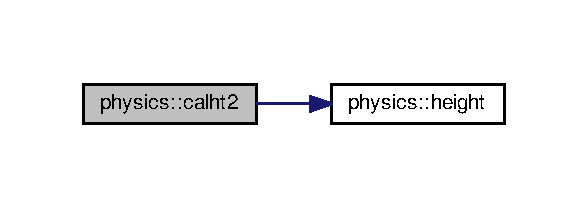
\includegraphics[width=282pt]{namespacephysics_a16ab28545ccd5528dd72f50208761dbe_cgraph}
\end{center}
\end{figure}




Here is the caller graph for this function\+:\nopagebreak
\begin{figure}[H]
\begin{center}
\leavevmode
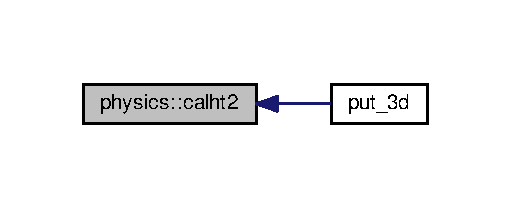
\includegraphics[width=245pt]{namespacephysics_a16ab28545ccd5528dd72f50208761dbe_icgraph}
\end{center}
\end{figure}


\index{physics@{physics}!diverg@{diverg}}
\index{diverg@{diverg}!physics@{physics}}
\subsubsection[{\texorpdfstring{diverg(\+U\+N\+I\+T\+H, V\+A\+R, U, V, D\+I\+V\+U, D\+I\+V\+V, D\+I\+V1)}{diverg(UNITH, VAR, U, V, DIVU, DIVV, DIV1)}}]{\setlength{\rightskip}{0pt plus 5cm}subroutine physics\+::diverg (
\begin{DoxyParamCaption}
\item[{real (kind=rk8), dimension(\+:), intent(in)}]{U\+N\+I\+TH, }
\item[{real (kind=rk8), dimension(\+:,\+:), intent(in)}]{V\+AR, }
\item[{real (kind=rk8), dimension(\+:,\+:), intent(in)}]{U, }
\item[{real (kind=rk8), dimension(\+:,\+:), intent(in)}]{V, }
\item[{real (kind=rk8), dimension(\+:,\+:), intent(in)}]{D\+I\+VU, }
\item[{real (kind=rk8), dimension(\+:,\+:), intent(in)}]{D\+I\+VV, }
\item[{real (kind=rk8), dimension(\+:), intent(out)}]{D\+I\+V1}
\end{DoxyParamCaption}
)}\hypertarget{namespacephysics_adc35216d512f6586071a79fba286a39c}{}\label{namespacephysics_adc35216d512f6586071a79fba286a39c}


Definition at line 170 of file physics.\+f90.


\begin{DoxyCode}
170 \textcolor{keywordtype}{USE }\hyperlink{namespaceportable}{portable}
171 
172 \textcolor{keywordtype}{IMPLICIT NONE}
173 \textcolor{keywordtype}{REAL (KIND=RK8)}, \textcolor{keywordtype}{DIMENSION(:)}, \textcolor{keywordtype}{INTENT(IN)}     :: unith      \textcolor{comment}{! One dimensional array with y columns.}
174 \textcolor{keywordtype}{REAL (KIND=RK8)}, \textcolor{keywordtype}{DIMENSION(:,:)}, \textcolor{keywordtype}{INTENT(IN)}   :: var        \textcolor{comment}{! Array with x columns and y rows containing
       the variable.}
175 \textcolor{keywordtype}{REAL (KIND=RK8)}, \textcolor{keywordtype}{DIMENSION(:,:)}, \textcolor{keywordtype}{INTENT(IN)}   :: u          \textcolor{comment}{! Array with x columns and y rows containing
       U-component of wind.}
176 \textcolor{keywordtype}{REAL (KIND=RK8)}, \textcolor{keywordtype}{DIMENSION(:,:)}, \textcolor{keywordtype}{INTENT(IN)}   :: v          \textcolor{comment}{! Array with x columns and y rows containing
       V-component of wind.}
177 \textcolor{keywordtype}{REAL (KIND=RK8)}, \textcolor{keywordtype}{DIMENSION(:,:)}, \textcolor{keywordtype}{INTENT(IN)}   :: divu       \textcolor{comment}{! Array with x columns and y rows containing
       DIVU.}
178 \textcolor{keywordtype}{REAL (KIND=RK8)}, \textcolor{keywordtype}{DIMENSION(:,:)}, \textcolor{keywordtype}{INTENT(IN)}   :: divv       \textcolor{comment}{! Array with x columns and y rows containing
       DIVV.}
179 \textcolor{keywordtype}{REAL (KIND=RK8)}, \textcolor{keywordtype}{DIMENSION(:)}, \textcolor{keywordtype}{INTENT(OUT)}    :: div1       \textcolor{comment}{! Array with x columns containing divergence.}
180 
181 div1    = matmul((u*var*divu + v*var*divv), unith)
182 
\end{DoxyCode}


Here is the caller graph for this function\+:\nopagebreak
\begin{figure}[H]
\begin{center}
\leavevmode
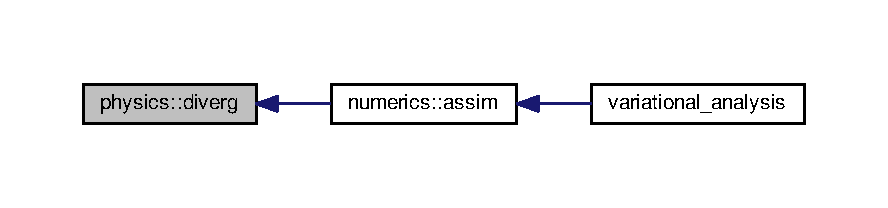
\includegraphics[width=350pt]{namespacephysics_adc35216d512f6586071a79fba286a39c_icgraph}
\end{center}
\end{figure}


\index{physics@{physics}!fcorlx@{fcorlx}}
\index{fcorlx@{fcorlx}!physics@{physics}}
\subsubsection[{\texorpdfstring{fcorlx(\+U\+N\+I\+T\+H, N\+S\+T\+U, F, V, F\+C\+X1)}{fcorlx(UNITH, NSTU, F, V, FCX1)}}]{\setlength{\rightskip}{0pt plus 5cm}subroutine physics\+::fcorlx (
\begin{DoxyParamCaption}
\item[{real (kind=rk8), dimension(nstu), intent(in)}]{U\+N\+I\+TH, }
\item[{integer(kind=ik4), intent(in)}]{N\+S\+TU, }
\item[{real (kind=rk8), dimension(\+:,\+:), intent(in)}]{F, }
\item[{real (kind=rk8), dimension(\+:,\+:), intent(in)}]{V, }
\item[{real (kind=rk8), dimension(\+:), intent(out)}]{F\+C\+X1}
\end{DoxyParamCaption}
)}\hypertarget{namespacephysics_a56a179b5bd2c13a2201b2367037a42cf}{}\label{namespacephysics_a56a179b5bd2c13a2201b2367037a42cf}


Definition at line 188 of file physics.\+f90.


\begin{DoxyCode}
188 \textcolor{keywordtype}{USE }\hyperlink{namespaceportable}{portable}
189 
190 \textcolor{keywordtype}{IMPLICIT NONE}
191 \textcolor{keywordtype}{INTEGER(KIND=IK4)}, \textcolor{keywordtype}{INTENT(IN)}                     :: nstu   \textcolor{comment}{! Number of stations}
192 \textcolor{keywordtype}{REAL (KIND=RK8)}, \textcolor{keywordtype}{DIMENSION(NSTU)}, \textcolor{keywordtype}{INTENT(IN)}      :: unith
193 \textcolor{keywordtype}{REAL (KIND=RK8)}, \textcolor{keywordtype}{DIMENSION(:,:)}, \textcolor{keywordtype}{INTENT(IN)}       :: f      \textcolor{comment}{! Coriolis parameter at each station and level.}
194 \textcolor{keywordtype}{REAL (KIND=RK8)}, \textcolor{keywordtype}{DIMENSION(:,:)}, \textcolor{keywordtype}{INTENT(IN)}       :: v      \textcolor{comment}{! V-wind component at each station and level.}
195 \textcolor{keywordtype}{REAL (KIND=RK8)}, \textcolor{keywordtype}{DIMENSION(:)}, \textcolor{keywordtype}{INTENT(OUT)}        :: fcx1
196 
197 fcx1    = matmul((v*f/nstu), unith)
198 
\end{DoxyCode}


Here is the caller graph for this function\+:\nopagebreak
\begin{figure}[H]
\begin{center}
\leavevmode
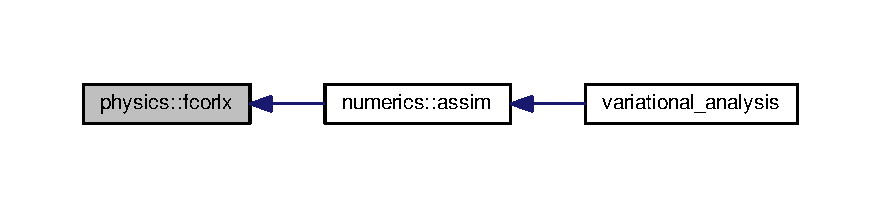
\includegraphics[width=350pt]{namespacephysics_a56a179b5bd2c13a2201b2367037a42cf_icgraph}
\end{center}
\end{figure}


\index{physics@{physics}!fcorly@{fcorly}}
\index{fcorly@{fcorly}!physics@{physics}}
\subsubsection[{\texorpdfstring{fcorly(\+U\+N\+I\+T\+H, N\+S\+T\+U, F, U, F\+C\+Y1)}{fcorly(UNITH, NSTU, F, U, FCY1)}}]{\setlength{\rightskip}{0pt plus 5cm}subroutine physics\+::fcorly (
\begin{DoxyParamCaption}
\item[{real (kind=rk8), dimension(nstu), intent(in)}]{U\+N\+I\+TH, }
\item[{integer(kind=ik4), intent(in)}]{N\+S\+TU, }
\item[{real (kind=rk8), dimension(\+:,\+:), intent(in)}]{F, }
\item[{real (kind=rk8), dimension(\+:,\+:), intent(in)}]{U, }
\item[{real (kind=rk8), dimension(\+:), intent(out)}]{F\+C\+Y1}
\end{DoxyParamCaption}
)}\hypertarget{namespacephysics_a1f64bd544ea55c7fbbf5330725fc0896}{}\label{namespacephysics_a1f64bd544ea55c7fbbf5330725fc0896}


Definition at line 204 of file physics.\+f90.


\begin{DoxyCode}
204 \textcolor{keywordtype}{USE }\hyperlink{namespaceportable}{portable}
205 
206 \textcolor{keywordtype}{IMPLICIT NONE}
207 \textcolor{keywordtype}{INTEGER(KIND=IK4)}, \textcolor{keywordtype}{INTENT(IN)}                     :: nstu   \textcolor{comment}{! Number of stations}
208 \textcolor{keywordtype}{REAL (KIND=RK8)}, \textcolor{keywordtype}{DIMENSION(NSTU)}, \textcolor{keywordtype}{INTENT(IN)}      :: unith
209 \textcolor{keywordtype}{REAL (KIND=RK8)}, \textcolor{keywordtype}{DIMENSION(:,:)}, \textcolor{keywordtype}{INTENT(IN)}       :: f      \textcolor{comment}{! Coriolis parameter at each station and level.}
210 \textcolor{keywordtype}{REAL (KIND=RK8)}, \textcolor{keywordtype}{DIMENSION(:,:)}, \textcolor{keywordtype}{INTENT(IN)}       :: u      \textcolor{comment}{! U-wind component at each station and level.}
211 \textcolor{keywordtype}{REAL (KIND=RK8)}, \textcolor{keywordtype}{DIMENSION(:)}, \textcolor{keywordtype}{INTENT(OUT)}        :: fcy1
212 
213 fcy1    = matmul((-u*f/nstu), unith)
214 
\end{DoxyCode}


Here is the caller graph for this function\+:\nopagebreak
\begin{figure}[H]
\begin{center}
\leavevmode
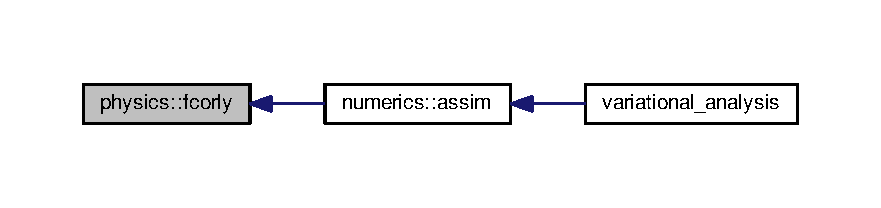
\includegraphics[width=350pt]{namespacephysics_a1f64bd544ea55c7fbbf5330725fc0896_icgraph}
\end{center}
\end{figure}


\index{physics@{physics}!fpgd@{fpgd}}
\index{fpgd@{fpgd}!physics@{physics}}
\subsubsection[{\texorpdfstring{fpgd(\+U\+N\+I\+T\+H, Z, D\+Z\+D\+X, F\+P1)}{fpgd(UNITH, Z, DZDX, FP1)}}]{\setlength{\rightskip}{0pt plus 5cm}subroutine physics\+::fpgd (
\begin{DoxyParamCaption}
\item[{real (kind=rk8), dimension(\+:), intent(in)}]{U\+N\+I\+TH, }
\item[{real (kind=rk8), dimension(\+:,\+:), intent(in)}]{Z, }
\item[{real (kind=rk8), dimension(\+:,\+:), intent(in)}]{D\+Z\+DX, }
\item[{real (kind=rk8), dimension(\+:), intent(out)}]{F\+P1}
\end{DoxyParamCaption}
)}\hypertarget{namespacephysics_acf841366af6f4fd7502b4031a2cacb56}{}\label{namespacephysics_acf841366af6f4fd7502b4031a2cacb56}


Definition at line 220 of file physics.\+f90.


\begin{DoxyCode}
220 \textcolor{keywordtype}{USE }\hyperlink{namespaceportable}{portable}
221 \textcolor{keywordtype}{USE }\hyperlink{namespaceconstants}{constants}
222 
223 \textcolor{keywordtype}{IMPLICIT NONE}
224 \textcolor{keywordtype}{REAL (KIND=RK8)}, \textcolor{keywordtype}{DIMENSION(:)}, \textcolor{keywordtype}{INTENT(IN)}     :: unith
225 \textcolor{keywordtype}{REAL (KIND=RK8)}, \textcolor{keywordtype}{DIMENSION(:,:)}, \textcolor{keywordtype}{INTENT(IN)}   :: z
226 \textcolor{keywordtype}{REAL (KIND=RK8)}, \textcolor{keywordtype}{DIMENSION(:,:)}, \textcolor{keywordtype}{INTENT(IN)}   :: dzdx
227 \textcolor{keywordtype}{REAL (KIND=RK8)}, \textcolor{keywordtype}{DIMENSION(:)}, \textcolor{keywordtype}{INTENT(OUT)}    :: fp1
228 
229 fp1 = matmul((-\hyperlink{namespaceconstants_a046aef138fbc8d05251d4fdc6eb3ee89}{g}*z*dzdx), unith)
230 
\end{DoxyCode}


Here is the caller graph for this function\+:\nopagebreak
\begin{figure}[H]
\begin{center}
\leavevmode
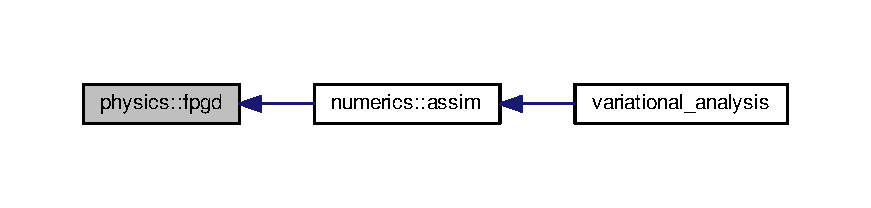
\includegraphics[width=350pt]{namespacephysics_acf841366af6f4fd7502b4031a2cacb56_icgraph}
\end{center}
\end{figure}


\index{physics@{physics}!height@{height}}
\index{height@{height}!physics@{physics}}
\subsubsection[{\texorpdfstring{height(\+N\+P, K\+S, K\+T, P, T, R, Z)}{height(NP, KS, KT, P, T, R, Z)}}]{\setlength{\rightskip}{0pt plus 5cm}subroutine physics\+::height (
\begin{DoxyParamCaption}
\item[{integer (kind=ik4), intent(in)}]{NP, }
\item[{integer (kind=ik4), intent(in)}]{KS, }
\item[{integer (kind=ik4), intent(in)}]{KT, }
\item[{real (kind=rk8), dimension(np), intent(in)}]{P, }
\item[{real (kind=rk8), dimension(np), intent(in)}]{T, }
\item[{real (kind=rk8), dimension(np), intent(in)}]{R, }
\item[{real (kind=rk8), dimension(np), intent(out)}]{Z}
\end{DoxyParamCaption}
)}\hypertarget{namespacephysics_a0ca41ce81224f2d7b292dc474c080c60}{}\label{namespacephysics_a0ca41ce81224f2d7b292dc474c080c60}


Definition at line 244 of file physics.\+f90.


\begin{DoxyCode}
244 \textcolor{keywordtype}{USE }\hyperlink{namespaceportable}{portable}
245 \textcolor{keywordtype}{USE }\hyperlink{namespaceconstants}{constants}
246 
247 \textcolor{keywordtype}{IMPLICIT NONE}
248 
249 \textcolor{keywordtype}{INTEGER (KIND=IK4)}, \textcolor{keywordtype}{INTENT(IN)}                :: np         \textcolor{comment}{! Number of pressure levels in the P, T, R and
       Z arrays.}
250 \textcolor{keywordtype}{INTEGER (KIND=IK4)}, \textcolor{keywordtype}{INTENT(IN)}                :: ks         \textcolor{comment}{! The level which the surface is at.}
251 \textcolor{keywordtype}{INTEGER (KIND=IK4)}, \textcolor{keywordtype}{INTENT(IN)}                :: kt         \textcolor{comment}{! Level at which the variational analysis
       stops.}
252 \textcolor{keywordtype}{REAL (KIND=RK8)}, \textcolor{keywordtype}{DIMENSION(NP)}, \textcolor{keywordtype}{INTENT(IN)}    :: p          \textcolor{comment}{! Pressure of each level.}
253 \textcolor{keywordtype}{REAL (KIND=RK8)}, \textcolor{keywordtype}{DIMENSION(NP)}, \textcolor{keywordtype}{INTENT(IN)}    :: t          \textcolor{comment}{! Temperature of each level.}
254 \textcolor{keywordtype}{REAL (KIND=RK8)}, \textcolor{keywordtype}{DIMENSION(NP)}, \textcolor{keywordtype}{INTENT(IN)}    :: r          \textcolor{comment}{! Mixing ratio at each level?}
255 \textcolor{keywordtype}{REAL (KIND=RK8)}, \textcolor{keywordtype}{DIMENSION(NP)}, \textcolor{keywordtype}{INTENT(OUT)}   :: z          \textcolor{comment}{! Geopotential height.}
256 
257 \textcolor{comment}{!}
258 \textcolor{comment}{! Local variables.}
259 \textcolor{comment}{!}
260 \textcolor{keywordtype}{REAL (KIND=RK8)}                               :: ep, r1, dz \textcolor{comment}{! Temporary variables.}
261 \textcolor{keywordtype}{INTEGER (KIND=IK4)}                            :: kk         \textcolor{comment}{! Counter.}
262 
263 ep  = \hyperlink{namespaceconstants_ad91564da82b97ea0d29ce0565565db85}{rd}/\hyperlink{namespaceconstants_a7ef8fc37397fbfbefd3c22883378dcc5}{rw}
264 
265 \textcolor{keywordflow}{DO} kk=ks+1,kt
266     r1      = \hyperlink{namespaceconstants_ad91564da82b97ea0d29ce0565565db85}{rd}*0.5*((1+r(kk-1)/ep)/(1+r(kk-1))+(1+r(kk)/ep)/(1+r(kk)))
267     dz      = r1/\hyperlink{namespaceconstants_a046aef138fbc8d05251d4fdc6eb3ee89}{g}*0.5*(t(kk-1)/p(kk-1)+t(kk)/p(kk))*(p(kk-1)-p(kk))
268     z(kk)   = z(kk-1)+dz
269 \textcolor{keywordflow}{END DO}
270 
\end{DoxyCode}


Here is the caller graph for this function\+:\nopagebreak
\begin{figure}[H]
\begin{center}
\leavevmode
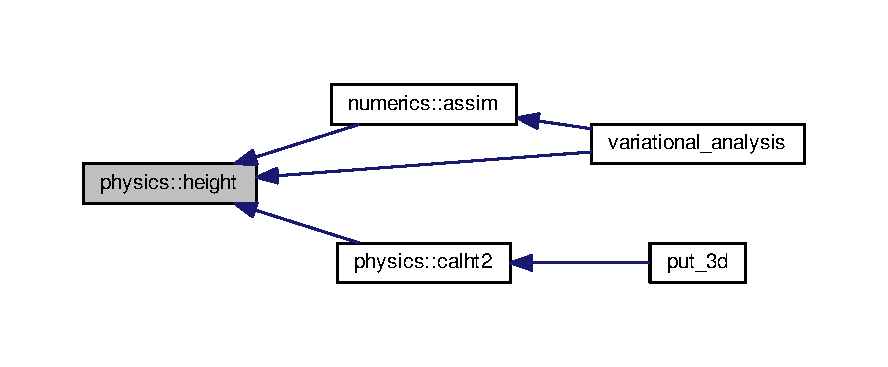
\includegraphics[width=350pt]{namespacephysics_a0ca41ce81224f2d7b292dc474c080c60_icgraph}
\end{center}
\end{figure}


\index{physics@{physics}!s\+\_\+r\+\_\+to\+\_\+t\+\_\+z@{s\+\_\+r\+\_\+to\+\_\+t\+\_\+z}}
\index{s\+\_\+r\+\_\+to\+\_\+t\+\_\+z@{s\+\_\+r\+\_\+to\+\_\+t\+\_\+z}!physics@{physics}}
\subsubsection[{\texorpdfstring{s\+\_\+r\+\_\+to\+\_\+t\+\_\+z(\+P, P\+S, Z\+S, S, R, T, Z)}{s_r_to_t_z(P, PS, ZS, S, R, T, Z)}}]{\setlength{\rightskip}{0pt plus 5cm}subroutine physics\+::s\+\_\+r\+\_\+to\+\_\+t\+\_\+z (
\begin{DoxyParamCaption}
\item[{real (kind=rk8), dimension(\+:), intent(in)}]{P, }
\item[{real (kind=rk8), intent(in)}]{PS, }
\item[{real (kind=rk8), intent(in)}]{ZS, }
\item[{real (kind=rk8), dimension(\+:), intent(in)}]{S, }
\item[{real (kind=rk8), dimension(\+:), intent(in)}]{R, }
\item[{real (kind=rk8), dimension(\+:), intent(out)}]{T, }
\item[{real (kind=rk8), dimension(\+:), intent(out)}]{Z}
\end{DoxyParamCaption}
)}\hypertarget{namespacephysics_a3f1959e7b3ff1a8d052f1e0441b1c379}{}\label{namespacephysics_a3f1959e7b3ff1a8d052f1e0441b1c379}


Definition at line 22 of file physics.\+f90.


\begin{DoxyCode}
22 \textcolor{keywordtype}{USE }\hyperlink{namespaceportable}{portable}
23 \textcolor{keywordtype}{USE }\hyperlink{namespaceconstants}{constants}
24 
25 \textcolor{keywordtype}{IMPLICIT NONE}
26 \textcolor{keywordtype}{REAL (KIND=RK8)}, \textcolor{keywordtype}{DIMENSION(:)}, \textcolor{keywordtype}{INTENT(IN)}       :: p    \textcolor{comment}{! Pressures of a vertical column (hPa)}
27 \textcolor{keywordtype}{REAL (KIND=RK8)}, \textcolor{keywordtype}{INTENT(IN)}                     :: ps   \textcolor{comment}{! Surface pressure (hPa)}
28 \textcolor{keywordtype}{REAL (KIND=RK8)}, \textcolor{keywordtype}{INTENT(IN)}                     :: zs   \textcolor{comment}{! Surface geopotential height (m)}
29 \textcolor{keywordtype}{REAL (KIND=RK8)}, \textcolor{keywordtype}{DIMENSION(:)}, \textcolor{keywordtype}{INTENT(IN)}       :: s    \textcolor{comment}{! (K)}
30 \textcolor{keywordtype}{REAL (KIND=RK8)}, \textcolor{keywordtype}{DIMENSION(:)}, \textcolor{keywordtype}{INTENT(IN)}       :: r    \textcolor{comment}{! Mixing ration (g/kg)}
31 \textcolor{keywordtype}{REAL (KIND=RK8)}, \textcolor{keywordtype}{DIMENSION(:)}, \textcolor{keywordtype}{INTENT(OUT)}      :: t    \textcolor{comment}{! Temperature at each level (K)}
32 \textcolor{keywordtype}{REAL (KIND=RK8)}, \textcolor{keywordtype}{DIMENSION(:)}, \textcolor{keywordtype}{INTENT(OUT)}      :: z    \textcolor{comment}{! Geopotential height at each level (m)}
33 
34 \textcolor{comment}{!}
35 \textcolor{comment}{! Local variables.}
36 \textcolor{comment}{!}
37 \textcolor{keywordtype}{REAL (KIND=RK8)}                                 :: g2       \textcolor{comment}{! 2*G}
38 \textcolor{keywordtype}{REAL (KIND=RK8)}                                 :: ep       \textcolor{comment}{! RD/RW}
39 \textcolor{keywordtype}{INTEGER (KIND=IK4)}                              :: ii       \textcolor{comment}{! Counter}
40 \textcolor{keywordtype}{REAL (KIND=RK8)}                                 :: rv, a1, p1, t1, r1, z1, p2, r2
41 
42 \textcolor{comment}{!}
43 \textcolor{comment}{! Assign and initialise some variables.}
44 \textcolor{comment}{!}
45 g2  = 2.0*\hyperlink{namespaceconstants_a046aef138fbc8d05251d4fdc6eb3ee89}{g}
46 ep  = \hyperlink{namespaceconstants_ad91564da82b97ea0d29ce0565565db85}{rd}/\hyperlink{namespaceconstants_a7ef8fc37397fbfbefd3c22883378dcc5}{rw}
47 t   = 0.0
48 z   = 0.0
49 
50 \textcolor{keywordflow}{WHERE} (p .GE. ps)
51     z   = zs
52     t   = s(1) - \hyperlink{namespaceconstants_a046aef138fbc8d05251d4fdc6eb3ee89}{g}*zs/\hyperlink{namespaceconstants_a32354adf3493f59d0fc17b0302b2c368}{cpd}
53 \textcolor{keywordflow}{END WHERE}
54 
55 p1  = ps
56 t1  = t(1)
57 r1  = r(1)
58 z1  = zs
59 
60 \textcolor{keywordflow}{DO} ii=transfer(maxloc(p, mask=p.LT.ps), 0),\textcolor{keyword}{SIZE}(p)
61     p2      = p(ii)
62     r2      = r(ii)
63     rv      = \hyperlink{namespaceconstants_ad91564da82b97ea0d29ce0565565db85}{rd}*0.5*((1+r1/ep)/(1+r1)+(1+r2/ep)/(1+r2))
64     a1      = rv/2.0/\hyperlink{namespaceconstants_a32354adf3493f59d0fc17b0302b2c368}{cpd}*log(p1/p2)
65     t(ii)   = (s(ii) - \hyperlink{namespaceconstants_a046aef138fbc8d05251d4fdc6eb3ee89}{g}/\hyperlink{namespaceconstants_a32354adf3493f59d0fc17b0302b2c368}{cpd}*z1 - a1*t1)/(1.0 + a1)
66     z(ii)   = z1 + rv*(t1+t(ii))/g2*log(p1/p2)
67 
68     p1      = p2
69     r1      = r2
70     z1      = z(ii)
71     t1      = t(ii)
72 \textcolor{keywordflow}{END DO}
73 
\end{DoxyCode}


Here is the caller graph for this function\+:\nopagebreak
\begin{figure}[H]
\begin{center}
\leavevmode
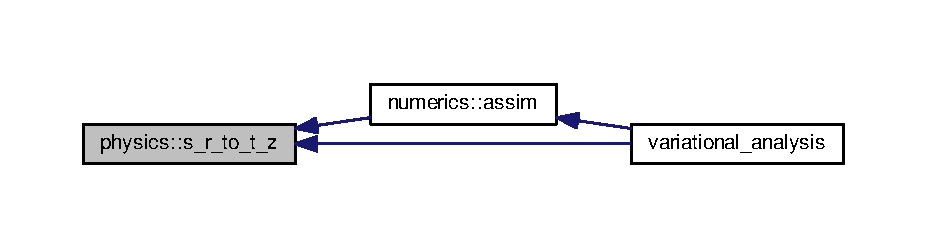
\includegraphics[width=350pt]{namespacephysics_a3f1959e7b3ff1a8d052f1e0441b1c379_icgraph}
\end{center}
\end{figure}


\index{physics@{physics}!t\+\_\+r\+\_\+to\+\_\+s\+\_\+z@{t\+\_\+r\+\_\+to\+\_\+s\+\_\+z}}
\index{t\+\_\+r\+\_\+to\+\_\+s\+\_\+z@{t\+\_\+r\+\_\+to\+\_\+s\+\_\+z}!physics@{physics}}
\subsubsection[{\texorpdfstring{t\+\_\+r\+\_\+to\+\_\+s\+\_\+z(\+P, P\+S, Z\+S, T, R, S, Z)}{t_r_to_s_z(P, PS, ZS, T, R, S, Z)}}]{\setlength{\rightskip}{0pt plus 5cm}subroutine physics\+::t\+\_\+r\+\_\+to\+\_\+s\+\_\+z (
\begin{DoxyParamCaption}
\item[{real (kind=rk8), dimension(\+:), intent(in)}]{P, }
\item[{real (kind=rk8), intent(in)}]{PS, }
\item[{real (kind=rk8), intent(in)}]{ZS, }
\item[{real (kind=rk8), dimension(\+:), intent(in)}]{T, }
\item[{real (kind=rk8), dimension(\+:), intent(in)}]{R, }
\item[{real (kind=rk8), dimension(\+:), intent(out)}]{S, }
\item[{real (kind=rk8), dimension(\+:), intent(out)}]{Z}
\end{DoxyParamCaption}
)}\hypertarget{namespacephysics_aebc42cd426e3ef8e85696bb1c7da18c3}{}\label{namespacephysics_aebc42cd426e3ef8e85696bb1c7da18c3}


Definition at line 87 of file physics.\+f90.


\begin{DoxyCode}
87 \textcolor{keywordtype}{USE }\hyperlink{namespaceportable}{portable}
88 \textcolor{keywordtype}{USE }\hyperlink{namespaceconstants}{constants}
89 
90 \textcolor{keywordtype}{IMPLICIT NONE}
91 \textcolor{keywordtype}{REAL (KIND=RK8)}, \textcolor{keywordtype}{INTENT(IN)}                             :: ps       \textcolor{comment}{! Surface pressure (hPa).}
92 \textcolor{keywordtype}{REAL (KIND=RK8)}, \textcolor{keywordtype}{INTENT(IN)}                             :: zs       \textcolor{comment}{! Surface geopotential height (m).}
93 \textcolor{keywordtype}{REAL (KIND=RK8)}, \textcolor{keywordtype}{DIMENSION(:)}, \textcolor{keywordtype}{INTENT(IN)}               :: p        \textcolor{comment}{! Pressure levels (hPa).}
94 \textcolor{keywordtype}{REAL (KIND=RK8)}, \textcolor{keywordtype}{DIMENSION(:)}, \textcolor{keywordtype}{INTENT(IN)}               :: t        \textcolor{comment}{! Temperature (K).}
95 \textcolor{keywordtype}{REAL (KIND=RK8)}, \textcolor{keywordtype}{DIMENSION(:)}, \textcolor{keywordtype}{INTENT(IN)}               :: r        \textcolor{comment}{! Mixing ration (g/kg).}
96 \textcolor{keywordtype}{REAL (KIND=RK8)}, \textcolor{keywordtype}{DIMENSION(:)}, \textcolor{keywordtype}{INTENT(OUT)}              :: s        \textcolor{comment}{! Dry static energy divided by CPD (K).}
97 \textcolor{keywordtype}{REAL (KIND=RK8)}, \textcolor{keywordtype}{DIMENSION(:)}, \textcolor{keywordtype}{INTENT(OUT)}              :: z        \textcolor{comment}{! Geopotential height (m).}
98 
99 \textcolor{comment}{!}
100 \textcolor{comment}{! Local variables.}
101 \textcolor{comment}{!}
102 \textcolor{keywordtype}{REAL (KIND=RK8)}                                         :: ep, g2, p1, t1, r1, p2, r2, t2, rv
103 \textcolor{keywordtype}{INTEGER (KIND=IK4)}                                      :: ll       \textcolor{comment}{! Counter.}
104 
105 \textcolor{comment}{!}
106 \textcolor{comment}{! Do some basic checks of the input data. This is an unfortunate necessity (otherwise bad input data can
       cause overflows in the}
107 \textcolor{comment}{! calculations. If bad data are detected, set the geopotential height and dry static energy to an undefined
       value (-9999.99)}
108 \textcolor{comment}{!}
109 
110 
111 
112 \textcolor{keywordflow}{IF} ((ps .LE. 0) .OR. (minval(p) .LE. 0) .OR. (minval(t) .LT. 0) .OR. (minval(r) .LT. 0)) \textcolor{keywordflow}{THEN}
113     s   = -9999.99
114     z   = -9999.99
115     \textcolor{keywordflow}{RETURN}
116 \textcolor{keywordflow}{END IF}
117 
118 \textcolor{comment}{!}
119 \textcolor{comment}{! Set some variables which are frequently used.}
120 \textcolor{comment}{!}
121 ep  = \hyperlink{namespaceconstants_ad91564da82b97ea0d29ce0565565db85}{rd}/\hyperlink{namespaceconstants_a7ef8fc37397fbfbefd3c22883378dcc5}{rw}
122 g2  = 2.0*\hyperlink{namespaceconstants_a046aef138fbc8d05251d4fdc6eb3ee89}{g}
123 
124 \textcolor{comment}{!}
125 \textcolor{comment}{! Where P is greater than PS, we are presumably below the surface. Set the geopotential height and dry
       static energy to surface}
126 \textcolor{comment}{! values. We also ensure the geopotential height of the lowest level is the same as the surface.}
127 \textcolor{comment}{!}
128 
129 z(1)    = zs
130 z       = 0
131 s       = 0
132 
133 \textcolor{keywordflow}{WHERE} (p .GE. ps)
134     z   = zs
135     s   = t(1) + \hyperlink{namespaceconstants_a046aef138fbc8d05251d4fdc6eb3ee89}{g}*zs/\hyperlink{namespaceconstants_a32354adf3493f59d0fc17b0302b2c368}{cpd}
136 \textcolor{keywordflow}{END WHERE}
137 
138 \textcolor{comment}{!}
139 \textcolor{comment}{! For each non-surface level, calculate the geopotential height and dry static energy.}
140 \textcolor{comment}{!}
141 p1  = ps
142 t1  = t(1)
143 r1  = r(1)
144 \textcolor{keywordflow}{DO} ll=max(1,transfer(maxloc(p, mask=p.LT.ps), 0)),\textcolor{keyword}{SIZE}(p)
145     p2      = p(ll)
146     t2      = t(ll)
147     r2      = r(ll)
148     rv      = \hyperlink{namespaceconstants_ad91564da82b97ea0d29ce0565565db85}{rd}*0.5*((1+r1/ep)/(1+r1) + (1+r2/ep)/(1+r2))
149     \textcolor{keywordflow}{IF} (ll.gt.1)  z(ll)   = z(ll-1) + rv*(t1+t2)/g2*log(p1/p2)
150     t1      = t2
151     p1      = p2
152     r1      = r2
153     s(ll)   = t(ll) + \hyperlink{namespaceconstants_a046aef138fbc8d05251d4fdc6eb3ee89}{g}*z(ll)/\hyperlink{namespaceconstants_a32354adf3493f59d0fc17b0302b2c368}{cpd}
154 \textcolor{keywordflow}{END DO}
155 
156 
\end{DoxyCode}


Here is the caller graph for this function\+:\nopagebreak
\begin{figure}[H]
\begin{center}
\leavevmode
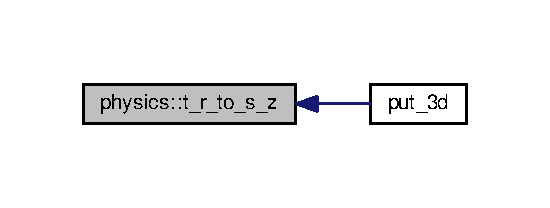
\includegraphics[width=264pt]{namespacephysics_aebc42cd426e3ef8e85696bb1c7da18c3_icgraph}
\end{center}
\end{figure}



\hypertarget{namespaceportable}{}\section{portable Module Reference}
\label{namespaceportable}\index{portable@{portable}}
\subsection*{Variables}
\begin{DoxyCompactItemize}
\item 
integer, parameter \hyperlink{namespaceportable_aaeaca599bf9baead529cbb42680f0f0b}{ik1} = S\+E\+L\+E\+C\+T\+E\+D\+\_\+\+I\+N\+T\+\_\+\+K\+I\+ND(2)
\item 
integer, parameter \hyperlink{namespaceportable_a35a0fbff20f9df8a8a5de95c97dc7d5d}{ik2} = S\+E\+L\+E\+C\+T\+E\+D\+\_\+\+I\+N\+T\+\_\+\+K\+I\+ND(4)
\item 
integer, parameter \hyperlink{namespaceportable_aa110cf333432508140602ea192c4b2ea}{ik4} = S\+E\+L\+E\+C\+T\+E\+D\+\_\+\+I\+N\+T\+\_\+\+K\+I\+ND(9)
\item 
integer, parameter \hyperlink{namespaceportable_abaed22a509442771d3fba69bebda0b33}{rk4} = S\+E\+L\+E\+C\+T\+E\+D\+\_\+\+R\+E\+A\+L\+\_\+\+K\+I\+ND(4, 30)
\item 
integer, parameter \hyperlink{namespaceportable_a609d4b38b4f128b310e288b1861ad9bd}{rk8} = S\+E\+L\+E\+C\+T\+E\+D\+\_\+\+R\+E\+A\+L\+\_\+\+K\+I\+ND(10, 200)
\end{DoxyCompactItemize}


\subsection{Variable Documentation}
\index{portable@{portable}!ik1@{ik1}}
\index{ik1@{ik1}!portable@{portable}}
\subsubsection[{\texorpdfstring{ik1}{ik1}}]{\setlength{\rightskip}{0pt plus 5cm}integer, parameter portable\+::ik1 = S\+E\+L\+E\+C\+T\+E\+D\+\_\+\+I\+N\+T\+\_\+\+K\+I\+ND(2)}\hypertarget{namespaceportable_aaeaca599bf9baead529cbb42680f0f0b}{}\label{namespaceportable_aaeaca599bf9baead529cbb42680f0f0b}


Definition at line 11 of file portable.\+f90.


\begin{DoxyCode}
11 \textcolor{keywordtype}{INTEGER}, \textcolor{keywordtype}{PARAMETER}  :: \hyperlink{namespaceportable_aaeaca599bf9baead529cbb42680f0f0b}{ik1} = selected\_int\_kind(2)       \textcolor{comment}{! Probably a 1 or 2 byte integer.}
\end{DoxyCode}
\index{portable@{portable}!ik2@{ik2}}
\index{ik2@{ik2}!portable@{portable}}
\subsubsection[{\texorpdfstring{ik2}{ik2}}]{\setlength{\rightskip}{0pt plus 5cm}integer, parameter portable\+::ik2 = S\+E\+L\+E\+C\+T\+E\+D\+\_\+\+I\+N\+T\+\_\+\+K\+I\+ND(4)}\hypertarget{namespaceportable_a35a0fbff20f9df8a8a5de95c97dc7d5d}{}\label{namespaceportable_a35a0fbff20f9df8a8a5de95c97dc7d5d}


Definition at line 12 of file portable.\+f90.


\begin{DoxyCode}
12 \textcolor{keywordtype}{INTEGER}, \textcolor{keywordtype}{PARAMETER}  :: \hyperlink{namespaceportable_a35a0fbff20f9df8a8a5de95c97dc7d5d}{ik2} = selected\_int\_kind(4)       \textcolor{comment}{! Probably a 2 byte integer.}
\end{DoxyCode}
\index{portable@{portable}!ik4@{ik4}}
\index{ik4@{ik4}!portable@{portable}}
\subsubsection[{\texorpdfstring{ik4}{ik4}}]{\setlength{\rightskip}{0pt plus 5cm}integer, parameter portable\+::ik4 = S\+E\+L\+E\+C\+T\+E\+D\+\_\+\+I\+N\+T\+\_\+\+K\+I\+ND(9)}\hypertarget{namespaceportable_aa110cf333432508140602ea192c4b2ea}{}\label{namespaceportable_aa110cf333432508140602ea192c4b2ea}


Definition at line 13 of file portable.\+f90.


\begin{DoxyCode}
13 \textcolor{keywordtype}{INTEGER}, \textcolor{keywordtype}{PARAMETER}  :: \hyperlink{namespaceportable_aa110cf333432508140602ea192c4b2ea}{ik4} = selected\_int\_kind(9)       \textcolor{comment}{! Probably a 4 byte integer.}
\end{DoxyCode}
\index{portable@{portable}!rk4@{rk4}}
\index{rk4@{rk4}!portable@{portable}}
\subsubsection[{\texorpdfstring{rk4}{rk4}}]{\setlength{\rightskip}{0pt plus 5cm}integer, parameter portable\+::rk4 = S\+E\+L\+E\+C\+T\+E\+D\+\_\+\+R\+E\+A\+L\+\_\+\+K\+I\+ND(4, 30)}\hypertarget{namespaceportable_abaed22a509442771d3fba69bebda0b33}{}\label{namespaceportable_abaed22a509442771d3fba69bebda0b33}


Definition at line 15 of file portable.\+f90.


\begin{DoxyCode}
15 \textcolor{keywordtype}{INTEGER}, \textcolor{keywordtype}{PARAMETER}  :: \hyperlink{namespaceportable_abaed22a509442771d3fba69bebda0b33}{rk4} = selected\_real\_kind(4,30)   \textcolor{comment}{! Probably a 4 byte real.}
\end{DoxyCode}
\index{portable@{portable}!rk8@{rk8}}
\index{rk8@{rk8}!portable@{portable}}
\subsubsection[{\texorpdfstring{rk8}{rk8}}]{\setlength{\rightskip}{0pt plus 5cm}integer, parameter portable\+::rk8 = S\+E\+L\+E\+C\+T\+E\+D\+\_\+\+R\+E\+A\+L\+\_\+\+K\+I\+ND(10, 200)}\hypertarget{namespaceportable_a609d4b38b4f128b310e288b1861ad9bd}{}\label{namespaceportable_a609d4b38b4f128b310e288b1861ad9bd}


Definition at line 17 of file portable.\+f90.


\begin{DoxyCode}
17 \textcolor{keywordtype}{INTEGER}, \textcolor{keywordtype}{PARAMETER}  :: \hyperlink{namespaceportable_a609d4b38b4f128b310e288b1861ad9bd}{rk8} = selected\_real\_kind(10,200) \textcolor{comment}{! Probably a 8 byte real.}
\end{DoxyCode}

\hypertarget{namespacesettings}{}\section{settings Module Reference}
\label{namespacesettings}\index{settings@{settings}}
\subsection*{Variables}
\begin{DoxyCompactItemize}
\item 
real(kind=rk8), parameter \hyperlink{namespacesettings_a80b5ece3c388ad5e0c924f372afebe65}{pstart} =200.\+0
\item 
real(kind=rk8), parameter \hyperlink{namespacesettings_a8d5e7d0c921e46fc4b2c7d7738729805}{pcrit} =200.\+0
\item 
integer(kind=ik4), parameter \hyperlink{namespacesettings_a78876a80ce867f4bc71866b783b6de89}{nvbudget\+\_\+column} =5
\item 
integer(kind=ik4), parameter \hyperlink{namespacesettings_a42675226258d1641f557f9e8e756b76e}{nvbudget\+\_\+layer} =6
\item 
integer(kind=ik4), parameter \hyperlink{namespacesettings_a3e7f9f832f20c3352f6a1c901bf3d13b}{ntermmax} =7
\item 
integer(kind=ik4), parameter \hyperlink{namespacesettings_acb91032130faf4bb56bee66af8cbf573}{ntermmaxv} =8
\item 
integer(kind=ik4), parameter \hyperlink{namespacesettings_a4f624be133b88a44c8976b47b85e8eec}{nad} =3
\item 
integer(kind=ik4), parameter \hyperlink{namespacesettings_a45f66b2df6e7509477bcf669702044a8}{nstx0} =10
\item 
integer(kind=ik4), parameter \hyperlink{namespacesettings_a3989615b44f5121ea2e8761d6abc24e1}{nsty0} =9
\item 
integer(kind=ik4), parameter \hyperlink{namespacesettings_a79e2ff19d589b215ed9176906dd5cbbf}{nvu} =10
\item 
integer(kind=ik4), parameter \hyperlink{namespacesettings_ac10106479d8b3db1c5edd195b8dbf36e}{nvs} = N\+VU
\item 
real(kind=rk8), parameter \hyperlink{namespacesettings_ac94cc887999dc993bb580baf0ce85ce3}{pt} =90.\+0
\item 
integer(kind=ik4), parameter \hyperlink{namespacesettings_a6feb18d2b9a31062fd7bc3f5533b0a4f}{start\+\_\+year} =2004
\item 
integer(kind=ik4), parameter \hyperlink{namespacesettings_a10988f9d662713f7f29e611c9b6c873d}{start\+\_\+month} =10
\item 
integer(kind=ik4), parameter \hyperlink{namespacesettings_a9d8f79c61533111bb5efd5ee1577108f}{start\+\_\+day} = 1
\end{DoxyCompactItemize}


\subsection{Variable Documentation}
\index{settings@{settings}!nad@{nad}}
\index{nad@{nad}!settings@{settings}}
\subsubsection[{\texorpdfstring{nad}{nad}}]{\setlength{\rightskip}{0pt plus 5cm}integer (kind=ik4), parameter settings\+::nad =3}\hypertarget{namespacesettings_a4f624be133b88a44c8976b47b85e8eec}{}\label{namespacesettings_a4f624be133b88a44c8976b47b85e8eec}


Definition at line 18 of file settings.\+f90.


\begin{DoxyCode}
18 \textcolor{keywordtype}{INTEGER (KIND=IK4)}, \textcolor{keywordtype}{PARAMETER}   :: \hyperlink{namespacesettings_a4f624be133b88a44c8976b47b85e8eec}{nad}=3                    \textcolor{comment}{! This controls which constraints are used
       in the analysis}
\end{DoxyCode}
\index{settings@{settings}!nstx0@{nstx0}}
\index{nstx0@{nstx0}!settings@{settings}}
\subsubsection[{\texorpdfstring{nstx0}{nstx0}}]{\setlength{\rightskip}{0pt plus 5cm}integer (kind=ik4), parameter settings\+::nstx0 =10}\hypertarget{namespacesettings_a45f66b2df6e7509477bcf669702044a8}{}\label{namespacesettings_a45f66b2df6e7509477bcf669702044a8}


Definition at line 22 of file settings.\+f90.


\begin{DoxyCode}
22 \textcolor{keywordtype}{INTEGER (KIND=IK4)}, \textcolor{keywordtype}{PARAMETER}   :: \hyperlink{namespacesettings_a45f66b2df6e7509477bcf669702044a8}{nstx0}=10                 \textcolor{comment}{! The X-size of a grid which covers the
       network (used in 2D\_PUT.F90).}
\end{DoxyCode}
\index{settings@{settings}!nsty0@{nsty0}}
\index{nsty0@{nsty0}!settings@{settings}}
\subsubsection[{\texorpdfstring{nsty0}{nsty0}}]{\setlength{\rightskip}{0pt plus 5cm}integer (kind=ik4), parameter settings\+::nsty0 =9}\hypertarget{namespacesettings_a3989615b44f5121ea2e8761d6abc24e1}{}\label{namespacesettings_a3989615b44f5121ea2e8761d6abc24e1}


Definition at line 23 of file settings.\+f90.


\begin{DoxyCode}
23 \textcolor{keywordtype}{INTEGER (KIND=IK4)}, \textcolor{keywordtype}{PARAMETER}   :: \hyperlink{namespacesettings_a3989615b44f5121ea2e8761d6abc24e1}{nsty0}=9                  \textcolor{comment}{! The Y-size of a grid which covers the
       network (used in 2D\_PUT.F90).}
\end{DoxyCode}
\index{settings@{settings}!ntermmax@{ntermmax}}
\index{ntermmax@{ntermmax}!settings@{settings}}
\subsubsection[{\texorpdfstring{ntermmax}{ntermmax}}]{\setlength{\rightskip}{0pt plus 5cm}integer (kind=ik4), parameter settings\+::ntermmax =7}\hypertarget{namespacesettings_a3e7f9f832f20c3352f6a1c901bf3d13b}{}\label{namespacesettings_a3e7f9f832f20c3352f6a1c901bf3d13b}


Definition at line 16 of file settings.\+f90.


\begin{DoxyCode}
16 \textcolor{keywordtype}{INTEGER (KIND=IK4)}, \textcolor{keywordtype}{PARAMETER}   :: \hyperlink{namespacesettings_a3e7f9f832f20c3352f6a1c901bf3d13b}{ntermmax}=7
\end{DoxyCode}
\index{settings@{settings}!ntermmaxv@{ntermmaxv}}
\index{ntermmaxv@{ntermmaxv}!settings@{settings}}
\subsubsection[{\texorpdfstring{ntermmaxv}{ntermmaxv}}]{\setlength{\rightskip}{0pt plus 5cm}integer (kind=ik4), parameter settings\+::ntermmaxv =8}\hypertarget{namespacesettings_acb91032130faf4bb56bee66af8cbf573}{}\label{namespacesettings_acb91032130faf4bb56bee66af8cbf573}


Definition at line 17 of file settings.\+f90.


\begin{DoxyCode}
17 \textcolor{keywordtype}{INTEGER (KIND=IK4)}, \textcolor{keywordtype}{PARAMETER}   :: \hyperlink{namespacesettings_acb91032130faf4bb56bee66af8cbf573}{ntermmaxv}=8
\end{DoxyCode}
\index{settings@{settings}!nvbudget\+\_\+column@{nvbudget\+\_\+column}}
\index{nvbudget\+\_\+column@{nvbudget\+\_\+column}!settings@{settings}}
\subsubsection[{\texorpdfstring{nvbudget\+\_\+column}{nvbudget_column}}]{\setlength{\rightskip}{0pt plus 5cm}integer (kind=ik4), parameter settings\+::nvbudget\+\_\+column =5}\hypertarget{namespacesettings_a78876a80ce867f4bc71866b783b6de89}{}\label{namespacesettings_a78876a80ce867f4bc71866b783b6de89}


Definition at line 14 of file settings.\+f90.


\begin{DoxyCode}
14 \textcolor{keywordtype}{INTEGER (KIND=IK4)}, \textcolor{keywordtype}{PARAMETER}   :: \hyperlink{namespacesettings_a78876a80ce867f4bc71866b783b6de89}{nvbudget\_column}=5
\end{DoxyCode}
\index{settings@{settings}!nvbudget\+\_\+layer@{nvbudget\+\_\+layer}}
\index{nvbudget\+\_\+layer@{nvbudget\+\_\+layer}!settings@{settings}}
\subsubsection[{\texorpdfstring{nvbudget\+\_\+layer}{nvbudget_layer}}]{\setlength{\rightskip}{0pt plus 5cm}integer (kind=ik4), parameter settings\+::nvbudget\+\_\+layer =6}\hypertarget{namespacesettings_a42675226258d1641f557f9e8e756b76e}{}\label{namespacesettings_a42675226258d1641f557f9e8e756b76e}


Definition at line 15 of file settings.\+f90.


\begin{DoxyCode}
15 \textcolor{keywordtype}{INTEGER (KIND=IK4)}, \textcolor{keywordtype}{PARAMETER}   :: \hyperlink{namespacesettings_a42675226258d1641f557f9e8e756b76e}{nvbudget\_layer}=6
\end{DoxyCode}
\index{settings@{settings}!nvs@{nvs}}
\index{nvs@{nvs}!settings@{settings}}
\subsubsection[{\texorpdfstring{nvs}{nvs}}]{\setlength{\rightskip}{0pt plus 5cm}integer (kind=ik4), parameter settings\+::nvs = N\+VU}\hypertarget{namespacesettings_ac10106479d8b3db1c5edd195b8dbf36e}{}\label{namespacesettings_ac10106479d8b3db1c5edd195b8dbf36e}


Definition at line 26 of file settings.\+f90.


\begin{DoxyCode}
26 \textcolor{keywordtype}{INTEGER (KIND=IK4)}, \textcolor{keywordtype}{PARAMETER}   :: \hyperlink{namespacesettings_ac10106479d8b3db1c5edd195b8dbf36e}{nvs}= \hyperlink{namespacesettings_a79e2ff19d589b215ed9176906dd5cbbf}{nvu}                 \textcolor{comment}{! Number of surface variables.}
\end{DoxyCode}
\index{settings@{settings}!nvu@{nvu}}
\index{nvu@{nvu}!settings@{settings}}
\subsubsection[{\texorpdfstring{nvu}{nvu}}]{\setlength{\rightskip}{0pt plus 5cm}integer (kind=ik4), parameter settings\+::nvu =10}\hypertarget{namespacesettings_a79e2ff19d589b215ed9176906dd5cbbf}{}\label{namespacesettings_a79e2ff19d589b215ed9176906dd5cbbf}


Definition at line 25 of file settings.\+f90.


\begin{DoxyCode}
25 \textcolor{keywordtype}{INTEGER (KIND=IK4)}, \textcolor{keywordtype}{PARAMETER}   :: \hyperlink{namespacesettings_a79e2ff19d589b215ed9176906dd5cbbf}{nvu}=10                   \textcolor{comment}{! Number of upper air variables.}
\end{DoxyCode}
\index{settings@{settings}!pcrit@{pcrit}}
\index{pcrit@{pcrit}!settings@{settings}}
\subsubsection[{\texorpdfstring{pcrit}{pcrit}}]{\setlength{\rightskip}{0pt plus 5cm}real (kind=rk8), parameter settings\+::pcrit =200.\+0}\hypertarget{namespacesettings_a8d5e7d0c921e46fc4b2c7d7738729805}{}\label{namespacesettings_a8d5e7d0c921e46fc4b2c7d7738729805}


Definition at line 12 of file settings.\+f90.


\begin{DoxyCode}
12 \textcolor{keywordtype}{REAL    (KIND=RK8)}, \textcolor{keywordtype}{PARAMETER}   :: \hyperlink{namespacesettings_a8d5e7d0c921e46fc4b2c7d7738729805}{pcrit}=200.0              \textcolor{comment}{! 200 hPa OK for the Tropics, no greater
       than 300 hPa for SGP.}
\end{DoxyCode}
\index{settings@{settings}!pstart@{pstart}}
\index{pstart@{pstart}!settings@{settings}}
\subsubsection[{\texorpdfstring{pstart}{pstart}}]{\setlength{\rightskip}{0pt plus 5cm}real (kind=rk8), parameter settings\+::pstart =200.\+0}\hypertarget{namespacesettings_a80b5ece3c388ad5e0c924f372afebe65}{}\label{namespacesettings_a80b5ece3c388ad5e0c924f372afebe65}


Definition at line 11 of file settings.\+f90.


\begin{DoxyCode}
11 \textcolor{keywordtype}{REAL    (KIND=RK8)}, \textcolor{keywordtype}{PARAMETER}   :: \hyperlink{namespacesettings_a80b5ece3c388ad5e0c924f372afebe65}{pstart}=200.0             \textcolor{comment}{! Where to start upper level filtering.
       Not currently used.}
\end{DoxyCode}
\index{settings@{settings}!pt@{pt}}
\index{pt@{pt}!settings@{settings}}
\subsubsection[{\texorpdfstring{pt}{pt}}]{\setlength{\rightskip}{0pt plus 5cm}real (kind=rk8), parameter settings\+::pt =90.\+0}\hypertarget{namespacesettings_ac94cc887999dc993bb580baf0ce85ce3}{}\label{namespacesettings_ac94cc887999dc993bb580baf0ce85ce3}


Definition at line 28 of file settings.\+f90.


\begin{DoxyCode}
28 \textcolor{keywordtype}{REAL (KIND=RK8)}, \textcolor{keywordtype}{PARAMETER}      :: \hyperlink{namespacesettings_ac94cc887999dc993bb580baf0ce85ce3}{pt}=90.0                  \textcolor{comment}{! Top of the variational analysis (hPa)}
\end{DoxyCode}
\index{settings@{settings}!start\+\_\+day@{start\+\_\+day}}
\index{start\+\_\+day@{start\+\_\+day}!settings@{settings}}
\subsubsection[{\texorpdfstring{start\+\_\+day}{start_day}}]{\setlength{\rightskip}{0pt plus 5cm}integer (kind=ik4), parameter settings\+::start\+\_\+day = 1}\hypertarget{namespacesettings_a9d8f79c61533111bb5efd5ee1577108f}{}\label{namespacesettings_a9d8f79c61533111bb5efd5ee1577108f}


Definition at line 31 of file settings.\+f90.


\begin{DoxyCode}
31 \textcolor{keywordtype}{INTEGER (KIND=IK4)}, \textcolor{keywordtype}{PARAMETER}   :: \hyperlink{namespacesettings_a9d8f79c61533111bb5efd5ee1577108f}{start\_day} = 1          \textcolor{comment}{! Start day for the variational
       analysis.}
\end{DoxyCode}
\index{settings@{settings}!start\+\_\+month@{start\+\_\+month}}
\index{start\+\_\+month@{start\+\_\+month}!settings@{settings}}
\subsubsection[{\texorpdfstring{start\+\_\+month}{start_month}}]{\setlength{\rightskip}{0pt plus 5cm}integer (kind=ik4), parameter settings\+::start\+\_\+month =10}\hypertarget{namespacesettings_a10988f9d662713f7f29e611c9b6c873d}{}\label{namespacesettings_a10988f9d662713f7f29e611c9b6c873d}


Definition at line 30 of file settings.\+f90.


\begin{DoxyCode}
30 \textcolor{keywordtype}{INTEGER (KIND=IK4)}, \textcolor{keywordtype}{PARAMETER}   :: \hyperlink{namespacesettings_a10988f9d662713f7f29e611c9b6c873d}{start\_month}=10          \textcolor{comment}{! Start month for the variational
       analysis.}
\end{DoxyCode}
\index{settings@{settings}!start\+\_\+year@{start\+\_\+year}}
\index{start\+\_\+year@{start\+\_\+year}!settings@{settings}}
\subsubsection[{\texorpdfstring{start\+\_\+year}{start_year}}]{\setlength{\rightskip}{0pt plus 5cm}integer (kind=ik4), parameter settings\+::start\+\_\+year =2004}\hypertarget{namespacesettings_a6feb18d2b9a31062fd7bc3f5533b0a4f}{}\label{namespacesettings_a6feb18d2b9a31062fd7bc3f5533b0a4f}


Definition at line 29 of file settings.\+f90.


\begin{DoxyCode}
29 \textcolor{keywordtype}{INTEGER (KIND=IK4)}, \textcolor{keywordtype}{PARAMETER}   :: \hyperlink{namespacesettings_a6feb18d2b9a31062fd7bc3f5533b0a4f}{start\_year}=2004          \textcolor{comment}{! Start year for the variational
       analysis.}
\end{DoxyCode}

\hypertarget{namespacesetup}{}\section{setup Namespace Reference}
\label{namespacesetup}\index{setup@{setup}}
\subsection*{Functions}
\begin{DoxyCompactItemize}
\item 
def \hyperlink{namespacesetup_a98c11c98a822ccbe47d135174bfcc346}{file\+\_\+search} (file)
\item 
def \hyperlink{namespacesetup_a3477c4ce4216a75efaf147946c414f4f}{checkenv} (var, alt)
\end{DoxyCompactItemize}
\subsection*{Variables}
\begin{DoxyCompactItemize}
\item 
\hyperlink{namespacesetup_ad8426f1e8d88dc4a6601f003805f9224}{Os} = platform.\+system()
\item 
\hyperlink{namespacesetup_a26e74581e39df55b9dbba8dcf7d485fe}{host} = socket.\+gethostname().lower()
\item 
float \hyperlink{namespacesetup_aea013977d24d48e57270f412b2c222c2}{sleep} = 0.\+2
\item 
string \hyperlink{namespacesetup_a299d8d9205ed54eac073b608d9ab6af8}{Path} = \textquotesingle{}/opt/local\textquotesingle{}
\item 
bool \hyperlink{namespacesetup_a5dd2d263367c323cbd4d063b156a4a68}{help} = True
\item 
string \hyperlink{namespacesetup_a2429357b780b7445dd4831250478d9ed}{txt}
\item 
\hyperlink{namespacesetup_aaadd587ba3f34c400f5df2cf05a7e1c5}{altnames} = dict(sed=\textquotesingle{}sed\textquotesingle{},awk=\textquotesingle{}awk\textquotesingle{},date=\textquotesingle{}date\textquotesingle{})
\item 
\hyperlink{namespacesetup_ac2fa2127d48feb1a28f2aafa6fd00d0b}{L\+D\+F\+L\+A\+GS} = L\+D\+F\+L\+A\+G\+S.\+split(\textquotesingle{},\textquotesingle{})
\item 
list \hyperlink{namespacesetup_a82d52368b879302df365513569195970}{missing\+\_\+package} = \mbox{[}$\,$\mbox{]}
\item 
tuple \hyperlink{namespacesetup_a38fd627eae7d93f3366e9b4f707e77dd}{checkbin}
\item 
\hyperlink{namespacesetup_ab82b87b5daf568d1c5c3c8fc41e52ca1}{status} = False
\item 
\hyperlink{namespacesetup_a501d41aa25b2969d3234702d4439c931}{fn}
\item 
list \hyperlink{namespacesetup_a9c08eb458bd1b35c49b4aeddb58b03af}{missing\+\_\+module} = \mbox{[}$\,$\mbox{]}
\item 
\hyperlink{namespacesetup_ada820daab4af8948c6a81a2bc70ec3e8}{method} = dict(pbs=\textquotesingle{}qsub\textquotesingle{},slurm=\textquotesingle{}sbatch\textquotesingle{})\mbox{[}\hyperlink{namespacesetup_a5c8a4998256b5c6d0700ac432fa75d4b}{B\+A\+T\+CH}\mbox{]}
\item 
\hyperlink{namespacesetup_a5c8a4998256b5c6d0700ac432fa75d4b}{B\+A\+T\+CH} = B\+A\+T\+C\+H.\+lower()
\item 
\hyperlink{namespacesetup_aac6afb4198c065254f41a7ce8297da6a}{proj\+\_\+file} = os.\+path.\+join(os.\+pardir,\textquotesingle{}.proj\textquotesingle{})
\item 
\hyperlink{namespacesetup_ac86422d915b07533937fc858abea97a4}{a} = raw\+\_\+input(\textquotesingle{}Warning option for creating batch jobs is set but no P\+R\+O\+J\+E\+CT if given, is that correct? \mbox{[}Y$\vert$n\mbox{]}\+: \textquotesingle{})
\item 
\hyperlink{namespacesetup_aea6945a959274b18887b0be79239ead7}{f} = open(\hyperlink{namespacesetup_aac6afb4198c065254f41a7ce8297da6a}{proj\+\_\+file},\textquotesingle{}w\textquotesingle{})
\item 
\hyperlink{namespacesetup_a4046afba70953007c6ba74e7d9c6bd5f}{M\+A\+IL} = raw\+\_\+input(\textquotesingle{}No user email is given, enter now\+: \textquotesingle{})
\item 
string \hyperlink{namespacesetup_accce39b4aa713fbb290144ec68f888af}{batch\+\_\+header} = u\char`\"{}\char`\"{}
\item 
string \hyperlink{namespacesetup_a86918b8c879471590485d8ac229362b2}{batch\+\_\+job}
\item 
\hyperlink{namespacesetup_a2331c56366b88428b33ad78c625cfcc8}{bash\+\_\+script} = os.\+path.\+join(os.\+pardir,\textquotesingle{}submit\+\_\+\%s.\+sh\textquotesingle{}\%\hyperlink{namespacesetup_a5c8a4998256b5c6d0700ac432fa75d4b}{B\+A\+T\+CH})
\item 
list \hyperlink{namespacesetup_a29c6bb44f4b88076bbd129b6114c9fd2}{version\+\_\+conflict} = \mbox{[}$\,$\mbox{]}
\item 
\hyperlink{namespacesetup_a27ac718b5c714e7f887a5769bb81e54e}{cmd} = \hyperlink{namespacesetup_aaadd587ba3f34c400f5df2cf05a7e1c5}{altnames}\mbox{[}command\mbox{]}
\item 
\hyperlink{namespacesetup_a46c1652bf2b2336d1bf166fc69cbb168}{process} = Popen(\mbox{[}\hyperlink{namespacesetup_a27ac718b5c714e7f887a5769bb81e54e}{cmd},\textquotesingle{}-\/-\/version\textquotesingle{}\mbox{]},stdout=P\+I\+PE)
\item 
\hyperlink{namespacesetup_a9a9fe68847ae604c87e0c586206415d9}{output}
\item 
\hyperlink{namespacesetup_ad9eccefc3ae62bb9f91bbbfa97900e49}{err}
\item 
\hyperlink{namespacesetup_a7e4d34412eadfa1481215bd61b81d64d}{exit\+\_\+code} = process.\+wait()
\item 
\hyperlink{namespacesetup_a8ebf34a9903eb2abbfbd92f17e3b89a4}{fl} = float(\textquotesingle{}.\textquotesingle{}.join(re.\+findall(r\textquotesingle{}\textbackslash{}d+\textquotesingle{},output.\+split(\textquotesingle{}\textbackslash{}n\textquotesingle{})\mbox{[}0\mbox{]})\mbox{[}0\+:2\mbox{]}))
\item 
string \hyperlink{namespacesetup_a11da39b62ca84bc7e300d60f43bf46a8}{makefile\+\_\+var}
\item 
string \hyperlink{namespacesetup_acdec383554bf7f66e8fe06336ebfca98}{makefile\+\_\+radar}
\end{DoxyCompactItemize}


\subsection{Function Documentation}
\index{setup@{setup}!checkenv@{checkenv}}
\index{checkenv@{checkenv}!setup@{setup}}
\subsubsection[{\texorpdfstring{checkenv(var, alt)}{checkenv(var, alt)}}]{\setlength{\rightskip}{0pt plus 5cm}def setup.\+checkenv (
\begin{DoxyParamCaption}
\item[{}]{var, }
\item[{}]{alt}
\end{DoxyParamCaption}
)}\hypertarget{namespacesetup_a3477c4ce4216a75efaf147946c414f4f}{}\label{namespacesetup_a3477c4ce4216a75efaf147946c414f4f}


Definition at line 26 of file setup.\+py.


\begin{DoxyCode}
26 \textcolor{keyword}{def }\hyperlink{namespacesetup_a3477c4ce4216a75efaf147946c414f4f}{checkenv}(var,alt):
27     \textcolor{keywordflow}{try}:
28         \textcolor{keywordflow}{return} os.environ[var]
29     \textcolor{keywordflow}{except} KeyError:
30         \textcolor{keywordflow}{return} alt
31 
32 \textcolor{comment}{#netcdfmod=os.popen('locate netcdf.mod 2> /dev/null').read().strip()}
33 
34 FC=\hyperlink{namespacesetup_a3477c4ce4216a75efaf147946c414f4f}{checkenv}(\textcolor{stringliteral}{'FC'},\textcolor{stringliteral}{'gfortran'})
35 CC=\hyperlink{namespacesetup_a3477c4ce4216a75efaf147946c414f4f}{checkenv}(\textcolor{stringliteral}{'CC'},\textcolor{stringliteral}{'gcc'})
36 FFLAGS=\hyperlink{namespacesetup_a3477c4ce4216a75efaf147946c414f4f}{checkenv}(\textcolor{stringliteral}{'FFLAGS'},\textcolor{stringliteral}{'-ffixed-line-length-0 -std=legacy -g -O3 -fimplicit-none -fsign-zero
       -fbounds-check -Wpedantic -fno-automatic'})
37 CFLAGS=\hyperlink{namespacesetup_a3477c4ce4216a75efaf147946c414f4f}{checkenv}(\textcolor{stringliteral}{'CFLAGS'},\textcolor{stringliteral}{'-O3 -Wpedantic'})
38 INCLUDE=\hyperlink{namespacesetup_a3477c4ce4216a75efaf147946c414f4f}{checkenv}(\textcolor{stringliteral}{'INCLUDE'},os.path.join(Path,\textcolor{stringliteral}{'include'})).replace(\textcolor{stringliteral}{':'},\textcolor{stringliteral}{','})
39 LDFLAGS=\hyperlink{namespacesetup_a3477c4ce4216a75efaf147946c414f4f}{checkenv}(\textcolor{stringliteral}{'LD\_LIBRARY\_PATH'},os.path.join(Path,\textcolor{stringliteral}{'lib'})).replace(\textcolor{stringliteral}{':'},\textcolor{stringliteral}{','})
40 FLIBS=\hyperlink{namespacesetup_a3477c4ce4216a75efaf147946c414f4f}{checkenv}(\textcolor{stringliteral}{'FLIBS'},\textcolor{stringliteral}{'netcdff'})
41 CLIBS=\hyperlink{namespacesetup_a3477c4ce4216a75efaf147946c414f4f}{checkenv}(\textcolor{stringliteral}{'CLIBS'},\textcolor{stringliteral}{'netcdf,m'})
42 BATCH=\hyperlink{namespacesetup_a3477c4ce4216a75efaf147946c414f4f}{checkenv}(\textcolor{stringliteral}{'BATCH'},0)
43 PROJECT=\hyperlink{namespacesetup_a3477c4ce4216a75efaf147946c414f4f}{checkenv}(\textcolor{stringliteral}{'PROJECT'},\textcolor{keywordtype}{None})
44 MAIL=\hyperlink{namespacesetup_a3477c4ce4216a75efaf147946c414f4f}{checkenv}(\textcolor{stringliteral}{'EMAIL'},\textcolor{stringliteral}{''})
45 PREFIX=os.path.dirname(os.path.dirname(os.path.abspath(\_\_file\_\_)))
46 \textcolor{comment}{#if len(netcdfmod):}
47 \textcolor{comment}{#    INCLUDE+=',%s'%os.path.dirname(netcdfmod)}
48 \textcolor{keywordflow}{try}:
49     ar=sys.argv[1:]
50     help=\textcolor{keyword}{False}
51     \textcolor{keywordflow}{for} b \textcolor{keywordflow}{in} ar:
52         a=b.replace(\textcolor{stringliteral}{'--'},\textcolor{stringliteral}{''}).upper()
53         \textcolor{keywordflow}{if} b.startswith(\textcolor{stringliteral}{'-h'}) \textcolor{keywordflow}{or} b.startswith(\textcolor{stringliteral}{'--h'}):
54             help=\textcolor{keyword}{True}
55         \textcolor{keywordflow}{if} b.lower().startswith(\textcolor{stringliteral}{'--prefix'}):
56             PREFIX = a.lower().split(\textcolor{stringliteral}{'='})[1]
57         \textcolor{keywordflow}{if} a.startswith(\textcolor{stringliteral}{'FC'}):
58             FC=a.split(\textcolor{stringliteral}{'='})[-1]
59         \textcolor{keywordflow}{if} a.startswith(\textcolor{stringliteral}{'FFLAGS'}):
60             FCFLAGS=a.split(\textcolor{stringliteral}{'='})[-1].replace(\textcolor{stringliteral}{','},\textcolor{stringliteral}{' '})
61         \textcolor{keywordflow}{if} a.startswith(\textcolor{stringliteral}{'CFLAGS'}):
62             CFLAGS=a.split(\textcolor{stringliteral}{'='})[-1].replace(\textcolor{stringliteral}{','},\textcolor{stringliteral}{' '})
63         \textcolor{keywordflow}{if} a.startswith(\textcolor{stringliteral}{'INCLUDE'}):
64             INCLUDE=a.split(\textcolor{stringliteral}{'='})[-1]
65         \textcolor{keywordflow}{if} a.startswith(\textcolor{stringliteral}{'LD\_LIBRARY\_PATH'}):
66             LDFLAGS=a.split(\textcolor{stringliteral}{'='})[-1]
67         \textcolor{keywordflow}{if} a.startswith(\textcolor{stringliteral}{'CLIBS'}):
68             CLIBS=a.split(\textcolor{stringliteral}{'='})[-1]
69         \textcolor{keywordflow}{if} a.startswith(\textcolor{stringliteral}{'FLIBS'}):
70             FLIBS=a.split(\textcolor{stringliteral}{'='})[-1]
71         \textcolor{keywordflow}{if} a.startswith(\textcolor{stringliteral}{'BATCH'}):
72             batch=a.split(\textcolor{stringliteral}{'='})[-1].lower()
73             \textcolor{keywordflow}{try} :
74               BATCH=\{\textcolor{stringliteral}{'p'}:\textcolor{stringliteral}{'pbs'},\textcolor{stringliteral}{'s'}:\textcolor{stringliteral}{'slurm'},\textcolor{stringliteral}{'ll'}:\textcolor{stringliteral}{'ll'}\}[batch[0]]
75             \textcolor{keywordflow}{except} KeyError:
76               sys.stderr.write(\textcolor{stringliteral}{'Batch option should be one of the following: pbs, slurm\(\backslash\)n'})
77               sys.exit(257)
78         \textcolor{keywordflow}{if} a.startswith(\textcolor{stringliteral}{'PROJECT'}):
79           PROJECT=a.split(\textcolor{stringliteral}{'='})[-1]
80         \textcolor{keywordflow}{if} a.startswith(\textcolor{stringliteral}{'EMAIL'}):
81           MAIL=a.split(\textcolor{stringliteral}{'='})[-1]
82 
\end{DoxyCode}
\index{setup@{setup}!file\+\_\+search@{file\+\_\+search}}
\index{file\+\_\+search@{file\+\_\+search}!setup@{setup}}
\subsubsection[{\texorpdfstring{file\+\_\+search(file)}{file_search(file)}}]{\setlength{\rightskip}{0pt plus 5cm}def setup.\+file\+\_\+search (
\begin{DoxyParamCaption}
\item[{}]{file}
\end{DoxyParamCaption}
)}\hypertarget{namespacesetup_a98c11c98a822ccbe47d135174bfcc346}{}\label{namespacesetup_a98c11c98a822ccbe47d135174bfcc346}


Definition at line 18 of file setup.\+py.


\begin{DoxyCode}
18 \textcolor{keyword}{def }\hyperlink{namespacesetup_a98c11c98a822ccbe47d135174bfcc346}{file\_search}(file):
19     time.sleep(sleep)
20     \textcolor{keywordflow}{for} path \textcolor{keywordflow}{in} os.environ[\textcolor{stringliteral}{'PATH'}].split(\textcolor{stringliteral}{':'}):
21         fn=os.path.join(path,file)
22         \textcolor{keywordflow}{if} os.path.isfile(os.path.join(path,fn)):
23             \textcolor{keywordflow}{return} \textcolor{keyword}{True},fn
24     \textcolor{keywordflow}{return} \textcolor{keyword}{False},\textcolor{keywordtype}{None}
25 
\end{DoxyCode}


\subsection{Variable Documentation}
\index{setup@{setup}!a@{a}}
\index{a@{a}!setup@{setup}}
\subsubsection[{\texorpdfstring{a}{a}}]{\setlength{\rightskip}{0pt plus 5cm}setup.\+a = raw\+\_\+input(\textquotesingle{}Warning option for creating batch jobs is set but no P\+R\+O\+J\+E\+CT if given, is that correct? \mbox{[}Y$\vert$n\mbox{]}\+: \textquotesingle{})}\hypertarget{namespacesetup_ac86422d915b07533937fc858abea97a4}{}\label{namespacesetup_ac86422d915b07533937fc858abea97a4}


Definition at line 201 of file setup.\+py.

\index{setup@{setup}!altnames@{altnames}}
\index{altnames@{altnames}!setup@{setup}}
\subsubsection[{\texorpdfstring{altnames}{altnames}}]{\setlength{\rightskip}{0pt plus 5cm}setup.\+altnames = dict(sed=\textquotesingle{}sed\textquotesingle{},awk=\textquotesingle{}awk\textquotesingle{},date=\textquotesingle{}date\textquotesingle{})}\hypertarget{namespacesetup_aaadd587ba3f34c400f5df2cf05a7e1c5}{}\label{namespacesetup_aaadd587ba3f34c400f5df2cf05a7e1c5}


Definition at line 142 of file setup.\+py.

\index{setup@{setup}!bash\+\_\+script@{bash\+\_\+script}}
\index{bash\+\_\+script@{bash\+\_\+script}!setup@{setup}}
\subsubsection[{\texorpdfstring{bash\+\_\+script}{bash_script}}]{\setlength{\rightskip}{0pt plus 5cm}setup.\+bash\+\_\+script = os.\+path.\+join(os.\+pardir,\textquotesingle{}submit\+\_\+\%s.\+sh\textquotesingle{}\%{\bf B\+A\+T\+CH})}\hypertarget{namespacesetup_a2331c56366b88428b33ad78c625cfcc8}{}\label{namespacesetup_a2331c56366b88428b33ad78c625cfcc8}


Definition at line 319 of file setup.\+py.

\index{setup@{setup}!B\+A\+T\+CH@{B\+A\+T\+CH}}
\index{B\+A\+T\+CH@{B\+A\+T\+CH}!setup@{setup}}
\subsubsection[{\texorpdfstring{B\+A\+T\+CH}{BATCH}}]{\setlength{\rightskip}{0pt plus 5cm}setup.\+B\+A\+T\+CH = B\+A\+T\+C\+H.\+lower()}\hypertarget{namespacesetup_a5c8a4998256b5c6d0700ac432fa75d4b}{}\label{namespacesetup_a5c8a4998256b5c6d0700ac432fa75d4b}


Definition at line 198 of file setup.\+py.

\index{setup@{setup}!batch\+\_\+header@{batch\+\_\+header}}
\index{batch\+\_\+header@{batch\+\_\+header}!setup@{setup}}
\subsubsection[{\texorpdfstring{batch\+\_\+header}{batch_header}}]{\setlength{\rightskip}{0pt plus 5cm}string setup.\+batch\+\_\+header = u\char`\"{}\char`\"{}}\hypertarget{namespacesetup_accce39b4aa713fbb290144ec68f888af}{}\label{namespacesetup_accce39b4aa713fbb290144ec68f888af}


Definition at line 212 of file setup.\+py.

\index{setup@{setup}!batch\+\_\+job@{batch\+\_\+job}}
\index{batch\+\_\+job@{batch\+\_\+job}!setup@{setup}}
\subsubsection[{\texorpdfstring{batch\+\_\+job}{batch_job}}]{\setlength{\rightskip}{0pt plus 5cm}setup.\+batch\+\_\+job}\hypertarget{namespacesetup_a86918b8c879471590485d8ac229362b2}{}\label{namespacesetup_a86918b8c879471590485d8ac229362b2}


Definition at line 240 of file setup.\+py.

\index{setup@{setup}!checkbin@{checkbin}}
\index{checkbin@{checkbin}!setup@{setup}}
\subsubsection[{\texorpdfstring{checkbin}{checkbin}}]{\setlength{\rightskip}{0pt plus 5cm}tuple setup.\+checkbin}\hypertarget{namespacesetup_a38fd627eae7d93f3366e9b4f707e77dd}{}\label{namespacesetup_a38fd627eae7d93f3366e9b4f707e77dd}
{\bfseries Initial value\+:}
\begin{DoxyCode}
1 = (\(\backslash\)
2         (\textcolor{stringliteral}{'gnu make'},\textcolor{stringliteral}{'make'},1),
3         (\textcolor{stringliteral}{'fortran compiler'},FC,1),
4         (\textcolor{stringliteral}{'nc-config'},\textcolor{stringliteral}{'nc-config'},1),
5         (\textcolor{stringliteral}{'ncap'},\textcolor{stringliteral}{'ncap'},1),
6         (\textcolor{stringliteral}{'ncatted'},\textcolor{stringliteral}{'ncatted'},1),
7         (\textcolor{stringliteral}{'ncbo'},\textcolor{stringliteral}{'ncbo'},1),
8         (\textcolor{stringliteral}{'ncdiff'},\textcolor{stringliteral}{'ncdiff'},1),
9         (\textcolor{stringliteral}{'ncdump'},\textcolor{stringliteral}{'ncdump'},1),
10         (\textcolor{stringliteral}{'ncea'},\textcolor{stringliteral}{'ncea'},1),
11         (\textcolor{stringliteral}{'ncecat'},\textcolor{stringliteral}{'ncecat'},1),
12         (\textcolor{stringliteral}{'nces'},\textcolor{stringliteral}{'nces'},1),
13         (\textcolor{stringliteral}{'ncgen'},\textcolor{stringliteral}{'ncgen'},1),
14         (\textcolor{stringliteral}{'ncks'},\textcolor{stringliteral}{'ncks'},1),
15         (\textcolor{stringliteral}{'ncrcat'},\textcolor{stringliteral}{'ncrcat'},1),
16         (\textcolor{stringliteral}{'ncrename'},\textcolor{stringliteral}{'ncrename'},1),
17         (\textcolor{stringliteral}{'ncwa'},\textcolor{stringliteral}{'ncwa'},1),
18         (\textcolor{stringliteral}{'date'},\textcolor{stringliteral}{'date'},2),
19         (\textcolor{stringliteral}{'awk'},\textcolor{stringliteral}{'awk'},2),
20         (\textcolor{stringliteral}{'sed'},\textcolor{stringliteral}{'sed'},2),
21         (\textcolor{stringliteral}{'gdl or idl'},\textcolor{stringliteral}{'gdl'},2)
22         )
\end{DoxyCode}


Definition at line 149 of file setup.\+py.

\index{setup@{setup}!cmd@{cmd}}
\index{cmd@{cmd}!setup@{setup}}
\subsubsection[{\texorpdfstring{cmd}{cmd}}]{\setlength{\rightskip}{0pt plus 5cm}setup.\+cmd = {\bf altnames}\mbox{[}command\mbox{]}}\hypertarget{namespacesetup_a27ac718b5c714e7f887a5769bb81e54e}{}\label{namespacesetup_a27ac718b5c714e7f887a5769bb81e54e}


Definition at line 350 of file setup.\+py.

\index{setup@{setup}!err@{err}}
\index{err@{err}!setup@{setup}}
\subsubsection[{\texorpdfstring{err}{err}}]{\setlength{\rightskip}{0pt plus 5cm}setup.\+err}\hypertarget{namespacesetup_ad9eccefc3ae62bb9f91bbbfa97900e49}{}\label{namespacesetup_ad9eccefc3ae62bb9f91bbbfa97900e49}


Definition at line 358 of file setup.\+py.

\index{setup@{setup}!exit\+\_\+code@{exit\+\_\+code}}
\index{exit\+\_\+code@{exit\+\_\+code}!setup@{setup}}
\subsubsection[{\texorpdfstring{exit\+\_\+code}{exit_code}}]{\setlength{\rightskip}{0pt plus 5cm}setup.\+exit\+\_\+code = process.\+wait()}\hypertarget{namespacesetup_a7e4d34412eadfa1481215bd61b81d64d}{}\label{namespacesetup_a7e4d34412eadfa1481215bd61b81d64d}


Definition at line 359 of file setup.\+py.

\index{setup@{setup}!f@{f}}
\index{f@{f}!setup@{setup}}
\subsubsection[{\texorpdfstring{f}{f}}]{\setlength{\rightskip}{0pt plus 5cm}setup.\+f = open({\bf proj\+\_\+file},\textquotesingle{}w\textquotesingle{})}\hypertarget{namespacesetup_aea6945a959274b18887b0be79239ead7}{}\label{namespacesetup_aea6945a959274b18887b0be79239ead7}


Definition at line 206 of file setup.\+py.

\index{setup@{setup}!fl@{fl}}
\index{fl@{fl}!setup@{setup}}
\subsubsection[{\texorpdfstring{fl}{fl}}]{\setlength{\rightskip}{0pt plus 5cm}setup.\+fl = float(\textquotesingle{}.\textquotesingle{}.join(re.\+findall(r\textquotesingle{}\textbackslash{}d+\textquotesingle{},output.\+split(\textquotesingle{}\textbackslash{}n\textquotesingle{})\mbox{[}0\mbox{]})\mbox{[}0\+:2\mbox{]}))}\hypertarget{namespacesetup_a8ebf34a9903eb2abbfbd92f17e3b89a4}{}\label{namespacesetup_a8ebf34a9903eb2abbfbd92f17e3b89a4}


Definition at line 360 of file setup.\+py.

\index{setup@{setup}!fn@{fn}}
\index{fn@{fn}!setup@{setup}}
\subsubsection[{\texorpdfstring{fn}{fn}}]{\setlength{\rightskip}{0pt plus 5cm}setup.\+fn}\hypertarget{namespacesetup_a501d41aa25b2969d3234702d4439c931}{}\label{namespacesetup_a501d41aa25b2969d3234702d4439c931}


Definition at line 175 of file setup.\+py.

\index{setup@{setup}!help@{help}}
\index{help@{help}!setup@{setup}}
\subsubsection[{\texorpdfstring{help}{help}}]{\setlength{\rightskip}{0pt plus 5cm}bool setup.\+help = True}\hypertarget{namespacesetup_a5dd2d263367c323cbd4d063b156a4a68}{}\label{namespacesetup_a5dd2d263367c323cbd4d063b156a4a68}


Definition at line 85 of file setup.\+py.

\index{setup@{setup}!host@{host}}
\index{host@{host}!setup@{setup}}
\subsubsection[{\texorpdfstring{host}{host}}]{\setlength{\rightskip}{0pt plus 5cm}string setup.\+host = socket.\+gethostname().lower()}\hypertarget{namespacesetup_a26e74581e39df55b9dbba8dcf7d485fe}{}\label{namespacesetup_a26e74581e39df55b9dbba8dcf7d485fe}


Definition at line 4 of file setup.\+py.

\index{setup@{setup}!L\+D\+F\+L\+A\+GS@{L\+D\+F\+L\+A\+GS}}
\index{L\+D\+F\+L\+A\+GS@{L\+D\+F\+L\+A\+GS}!setup@{setup}}
\subsubsection[{\texorpdfstring{L\+D\+F\+L\+A\+GS}{LDFLAGS}}]{\setlength{\rightskip}{0pt plus 5cm}setup.\+L\+D\+F\+L\+A\+GS = L\+D\+F\+L\+A\+G\+S.\+split(\textquotesingle{},\textquotesingle{})}\hypertarget{namespacesetup_ac2fa2127d48feb1a28f2aafa6fd00d0b}{}\label{namespacesetup_ac2fa2127d48feb1a28f2aafa6fd00d0b}


Definition at line 144 of file setup.\+py.

\index{setup@{setup}!M\+A\+IL@{M\+A\+IL}}
\index{M\+A\+IL@{M\+A\+IL}!setup@{setup}}
\subsubsection[{\texorpdfstring{M\+A\+IL}{MAIL}}]{\setlength{\rightskip}{0pt plus 5cm}setup.\+M\+A\+IL = raw\+\_\+input(\textquotesingle{}No user email is given, enter now\+: \textquotesingle{})}\hypertarget{namespacesetup_a4046afba70953007c6ba74e7d9c6bd5f}{}\label{namespacesetup_a4046afba70953007c6ba74e7d9c6bd5f}


Definition at line 210 of file setup.\+py.

\index{setup@{setup}!makefile\+\_\+radar@{makefile\+\_\+radar}}
\index{makefile\+\_\+radar@{makefile\+\_\+radar}!setup@{setup}}
\subsubsection[{\texorpdfstring{makefile\+\_\+radar}{makefile_radar}}]{\setlength{\rightskip}{0pt plus 5cm}string setup.\+makefile\+\_\+radar}\hypertarget{namespacesetup_acdec383554bf7f66e8fe06336ebfca98}{}\label{namespacesetup_acdec383554bf7f66e8fe06336ebfca98}


Definition at line 466 of file setup.\+py.

\index{setup@{setup}!makefile\+\_\+var@{makefile\+\_\+var}}
\index{makefile\+\_\+var@{makefile\+\_\+var}!setup@{setup}}
\subsubsection[{\texorpdfstring{makefile\+\_\+var}{makefile_var}}]{\setlength{\rightskip}{0pt plus 5cm}string setup.\+makefile\+\_\+var}\hypertarget{namespacesetup_a11da39b62ca84bc7e300d60f43bf46a8}{}\label{namespacesetup_a11da39b62ca84bc7e300d60f43bf46a8}


Definition at line 391 of file setup.\+py.

\index{setup@{setup}!method@{method}}
\index{method@{method}!setup@{setup}}
\subsubsection[{\texorpdfstring{method}{method}}]{\setlength{\rightskip}{0pt plus 5cm}setup.\+method = dict(pbs=\textquotesingle{}qsub\textquotesingle{},slurm=\textquotesingle{}sbatch\textquotesingle{})\mbox{[}{\bf B\+A\+T\+CH}\mbox{]}}\hypertarget{namespacesetup_ada820daab4af8948c6a81a2bc70ec3e8}{}\label{namespacesetup_ada820daab4af8948c6a81a2bc70ec3e8}


Definition at line 197 of file setup.\+py.

\index{setup@{setup}!missing\+\_\+module@{missing\+\_\+module}}
\index{missing\+\_\+module@{missing\+\_\+module}!setup@{setup}}
\subsubsection[{\texorpdfstring{missing\+\_\+module}{missing_module}}]{\setlength{\rightskip}{0pt plus 5cm}list setup.\+missing\+\_\+module = \mbox{[}$\,$\mbox{]}}\hypertarget{namespacesetup_a9c08eb458bd1b35c49b4aeddb58b03af}{}\label{namespacesetup_a9c08eb458bd1b35c49b4aeddb58b03af}


Definition at line 195 of file setup.\+py.

\index{setup@{setup}!missing\+\_\+package@{missing\+\_\+package}}
\index{missing\+\_\+package@{missing\+\_\+package}!setup@{setup}}
\subsubsection[{\texorpdfstring{missing\+\_\+package}{missing_package}}]{\setlength{\rightskip}{0pt plus 5cm}list setup.\+missing\+\_\+package = \mbox{[}$\,$\mbox{]}}\hypertarget{namespacesetup_a82d52368b879302df365513569195970}{}\label{namespacesetup_a82d52368b879302df365513569195970}


Definition at line 147 of file setup.\+py.

\index{setup@{setup}!Os@{Os}}
\index{Os@{Os}!setup@{setup}}
\subsubsection[{\texorpdfstring{Os}{Os}}]{\setlength{\rightskip}{0pt plus 5cm}string setup.\+Os = platform.\+system()}\hypertarget{namespacesetup_ad8426f1e8d88dc4a6601f003805f9224}{}\label{namespacesetup_ad8426f1e8d88dc4a6601f003805f9224}


Definition at line 3 of file setup.\+py.

\index{setup@{setup}!output@{output}}
\index{output@{output}!setup@{setup}}
\subsubsection[{\texorpdfstring{output}{output}}]{\setlength{\rightskip}{0pt plus 5cm}setup.\+output}\hypertarget{namespacesetup_a9a9fe68847ae604c87e0c586206415d9}{}\label{namespacesetup_a9a9fe68847ae604c87e0c586206415d9}


Definition at line 358 of file setup.\+py.

\index{setup@{setup}!Path@{Path}}
\index{Path@{Path}!setup@{setup}}
\subsubsection[{\texorpdfstring{Path}{Path}}]{\setlength{\rightskip}{0pt plus 5cm}string setup.\+Path = \textquotesingle{}/opt/local\textquotesingle{}}\hypertarget{namespacesetup_a299d8d9205ed54eac073b608d9ab6af8}{}\label{namespacesetup_a299d8d9205ed54eac073b608d9ab6af8}


Definition at line 13 of file setup.\+py.

\index{setup@{setup}!process@{process}}
\index{process@{process}!setup@{setup}}
\subsubsection[{\texorpdfstring{process}{process}}]{\setlength{\rightskip}{0pt plus 5cm}setup.\+process = Popen(\mbox{[}{\bf cmd},\textquotesingle{}-\/-\/version\textquotesingle{}\mbox{]},stdout=P\+I\+PE)}\hypertarget{namespacesetup_a46c1652bf2b2336d1bf166fc69cbb168}{}\label{namespacesetup_a46c1652bf2b2336d1bf166fc69cbb168}


Definition at line 357 of file setup.\+py.

\index{setup@{setup}!proj\+\_\+file@{proj\+\_\+file}}
\index{proj\+\_\+file@{proj\+\_\+file}!setup@{setup}}
\subsubsection[{\texorpdfstring{proj\+\_\+file}{proj_file}}]{\setlength{\rightskip}{0pt plus 5cm}setup.\+proj\+\_\+file = os.\+path.\+join(os.\+pardir,\textquotesingle{}.proj\textquotesingle{})}\hypertarget{namespacesetup_aac6afb4198c065254f41a7ce8297da6a}{}\label{namespacesetup_aac6afb4198c065254f41a7ce8297da6a}


Definition at line 199 of file setup.\+py.

\index{setup@{setup}!sleep@{sleep}}
\index{sleep@{sleep}!setup@{setup}}
\subsubsection[{\texorpdfstring{sleep}{sleep}}]{\setlength{\rightskip}{0pt plus 5cm}float setup.\+sleep = 0.\+2}\hypertarget{namespacesetup_aea013977d24d48e57270f412b2c222c2}{}\label{namespacesetup_aea013977d24d48e57270f412b2c222c2}


Definition at line 10 of file setup.\+py.

\index{setup@{setup}!status@{status}}
\index{status@{status}!setup@{setup}}
\subsubsection[{\texorpdfstring{status}{status}}]{\setlength{\rightskip}{0pt plus 5cm}bool setup.\+status = False}\hypertarget{namespacesetup_ab82b87b5daf568d1c5c3c8fc41e52ca1}{}\label{namespacesetup_ab82b87b5daf568d1c5c3c8fc41e52ca1}


Definition at line 175 of file setup.\+py.

\index{setup@{setup}!txt@{txt}}
\index{txt@{txt}!setup@{setup}}
\subsubsection[{\texorpdfstring{txt}{txt}}]{\setlength{\rightskip}{0pt plus 5cm}string setup.\+txt}\hypertarget{namespacesetup_a2429357b780b7445dd4831250478d9ed}{}\label{namespacesetup_a2429357b780b7445dd4831250478d9ed}


Definition at line 86 of file setup.\+py.

\index{setup@{setup}!version\+\_\+conflict@{version\+\_\+conflict}}
\index{version\+\_\+conflict@{version\+\_\+conflict}!setup@{setup}}
\subsubsection[{\texorpdfstring{version\+\_\+conflict}{version_conflict}}]{\setlength{\rightskip}{0pt plus 5cm}list setup.\+version\+\_\+conflict = \mbox{[}$\,$\mbox{]}}\hypertarget{namespacesetup_a29c6bb44f4b88076bbd129b6114c9fd2}{}\label{namespacesetup_a29c6bb44f4b88076bbd129b6114c9fd2}


Definition at line 347 of file setup.\+py.


\hypertarget{namespacetime}{}\section{time Module Reference}
\label{namespacetime}\index{time@{time}}
\subsection*{Functions/\+Subroutines}
\begin{DoxyCompactItemize}
\item 
subroutine \hyperlink{namespacetime_a29670e6cf798cee7d9e33201b38f9507}{days\+\_\+to\+\_\+date} (S\+T\+Y\+E\+AR, S\+T\+M\+O\+N\+TH, S\+T\+D\+AY, D\+A\+YS, Y\+Y\+YY, MO, DD, HH, MM, SS)
\item 
integer(kind=ik4) function \hyperlink{namespacetime_a7c66adfc707644b0644b33e1557f1486}{date\+\_\+time\+\_\+to\+\_\+unix} (Y\+Y\+YY, MO, DD, HH, MM, SS)
\item 
logical function \hyperlink{namespacetime_ac7f82d40fd2b49e7e9025b103e88555c}{leapyear} (Y\+E\+AR)
\end{DoxyCompactItemize}


\subsection{Function/\+Subroutine Documentation}
\index{time@{time}!date\+\_\+time\+\_\+to\+\_\+unix@{date\+\_\+time\+\_\+to\+\_\+unix}}
\index{date\+\_\+time\+\_\+to\+\_\+unix@{date\+\_\+time\+\_\+to\+\_\+unix}!time@{time}}
\subsubsection[{\texorpdfstring{date\+\_\+time\+\_\+to\+\_\+unix(\+Y\+Y\+Y\+Y, M\+O, D\+D, H\+H, M\+M, S\+S)}{date_time_to_unix(YYYY, MO, DD, HH, MM, SS)}}]{\setlength{\rightskip}{0pt plus 5cm}integer (kind=ik4) function time\+::date\+\_\+time\+\_\+to\+\_\+unix (
\begin{DoxyParamCaption}
\item[{integer (kind=ik4), intent(in), optional}]{Y\+Y\+YY, }
\item[{integer (kind=ik4), intent(in), optional}]{MO, }
\item[{integer (kind=ik4), intent(in), optional}]{DD, }
\item[{integer (kind=ik4), intent(in), optional}]{HH, }
\item[{integer (kind=ik4), intent(in), optional}]{MM, }
\item[{integer (kind=ik4), intent(in), optional}]{SS}
\end{DoxyParamCaption}
)}\hypertarget{namespacetime_a7c66adfc707644b0644b33e1557f1486}{}\label{namespacetime_a7c66adfc707644b0644b33e1557f1486}


Definition at line 90 of file time.\+f90.


\begin{DoxyCode}
90 
91 \textcolor{keywordtype}{INTEGER (KIND=IK4)}, \textcolor{keywordtype}{INTENT(IN)}, \textcolor{keywordtype}{OPTIONAL}    :: yyyy                     \textcolor{comment}{! The year.}
92 \textcolor{keywordtype}{INTEGER (KIND=IK4)}, \textcolor{keywordtype}{INTENT(IN)}, \textcolor{keywordtype}{OPTIONAL}    :: mo                       \textcolor{comment}{! The month.}
93 \textcolor{keywordtype}{INTEGER (KIND=IK4)}, \textcolor{keywordtype}{INTENT(IN)}, \textcolor{keywordtype}{OPTIONAL}    :: dd                       \textcolor{comment}{! The day.}
94 \textcolor{keywordtype}{INTEGER (KIND=IK4)}, \textcolor{keywordtype}{INTENT(IN)}, \textcolor{keywordtype}{OPTIONAL}    :: hh                       \textcolor{comment}{! The hour.}
95 \textcolor{keywordtype}{INTEGER (KIND=IK4)}, \textcolor{keywordtype}{INTENT(IN)}, \textcolor{keywordtype}{OPTIONAL}    :: mm                       \textcolor{comment}{! The minute.}
96 \textcolor{keywordtype}{INTEGER (KIND=IK4)}, \textcolor{keywordtype}{INTENT(IN)}, \textcolor{keywordtype}{OPTIONAL}    :: ss                       \textcolor{comment}{! The second.}
97 
98 \textcolor{keywordtype}{INTEGER (KIND=IK4)}, \textcolor{keywordtype}{DIMENSION(6)}            :: datetime                 \textcolor{comment}{! Parts of the date and time.}
99 \textcolor{keywordtype}{INTEGER (KIND=IK4)}                          :: yycnt                    \textcolor{comment}{! Year counter.}
100 \textcolor{keywordtype}{INTEGER (KIND=IK4)}                          :: mocnt                    \textcolor{comment}{! Month counter.}
101 \textcolor{keywordtype}{INTEGER (KIND=IK4)}, \textcolor{keywordtype}{DIMENSION(12)}           :: mdays = (/ 31, 28, 31, 30, 31, 30, 31, 31, 30, 31, 30, 31 /)
102 \textcolor{keywordtype}{INTEGER (KIND=IK4)}                          :: utime                    \textcolor{comment}{! UNIX time.}
103 
104 \textcolor{comment}{!}
105 \textcolor{comment}{! Set the date and time parts (and use default values if they are not specified by the user).}
106 \textcolor{comment}{!}
107 \textcolor{keywordflow}{IF} (\textcolor{keyword}{PRESENT}(yyyy)) \textcolor{keywordflow}{THEN}
108     datetime(1) = yyyy
109 \textcolor{keywordflow}{ELSE}
110     datetime(1) = 1970
111 \textcolor{keywordflow}{ENDIF}
112 
113 \textcolor{keywordflow}{IF} (\textcolor{keyword}{PRESENT}(mo)) \textcolor{keywordflow}{THEN}
114     datetime(2) = mo
115 \textcolor{keywordflow}{ELSE}
116     datetime(2) = 1
117 \textcolor{keywordflow}{ENDIF}
118 
119 \textcolor{keywordflow}{IF} (\textcolor{keyword}{PRESENT}(dd)) \textcolor{keywordflow}{THEN}
120     datetime(3) = dd
121 \textcolor{keywordflow}{ELSE}
122     datetime(3) = 1
123 \textcolor{keywordflow}{ENDIF}
124 
125 \textcolor{keywordflow}{IF} (\textcolor{keyword}{PRESENT}(hh)) \textcolor{keywordflow}{THEN}
126     datetime(4) = hh
127 \textcolor{keywordflow}{ELSE}
128     datetime(4) = 0
129 \textcolor{keywordflow}{ENDIF}
130 
131 \textcolor{keywordflow}{IF} (\textcolor{keyword}{PRESENT}(mm)) \textcolor{keywordflow}{THEN}
132     datetime(5) = mm
133 \textcolor{keywordflow}{ELSE}
134     datetime(5) = 0
135 \textcolor{keywordflow}{ENDIF}
136 
137 \textcolor{keywordflow}{IF} (\textcolor{keyword}{PRESENT}(ss)) \textcolor{keywordflow}{THEN}
138     datetime(6) = ss
139 \textcolor{keywordflow}{ELSE}
140     datetime(6) = 0
141 \textcolor{keywordflow}{ENDIF}
142 
143 \textcolor{comment}{!}
144 \textcolor{comment}{! Check inputs are valid.}
145 \textcolor{comment}{!}
146 \textcolor{keywordflow}{IF} ((datetime(1) .LT. 1970) .OR. (datetime(1) .GT. 2037)) \textcolor{keywordflow}{THEN}
147     print *, \textcolor{stringliteral}{'W: Year is out of range (1970-2037)'}
148     \hyperlink{namespacetime_a7c66adfc707644b0644b33e1557f1486}{date\_time\_to\_unix}   = -1
149     \textcolor{keywordflow}{RETURN}
150 \textcolor{keywordflow}{ENDIF}
151 
152 \textcolor{keywordflow}{IF} ((datetime(2) .LT. 1) .OR. (datetime(2) .GT. 12)) \textcolor{keywordflow}{THEN}
153     print *, \textcolor{stringliteral}{'W: Month is out of range (1-12)'}
154     \hyperlink{namespacetime_a7c66adfc707644b0644b33e1557f1486}{date\_time\_to\_unix}   = -1
155     \textcolor{keywordflow}{RETURN}
156 \textcolor{keywordflow}{ENDIF}
157 
158 \textcolor{keywordflow}{IF} (\hyperlink{namespacetime_ac7f82d40fd2b49e7e9025b103e88555c}{leapyear}(datetime(1))) \textcolor{keywordflow}{THEN}     \textcolor{comment}{! We'll use these results later as well.}
159     mdays(2)    = 29
160 \textcolor{keywordflow}{ELSE}
161     mdays(2)    = 28
162 \textcolor{keywordflow}{ENDIF}
163 \textcolor{keywordflow}{IF} ((datetime(3) .LT. 1) .OR. (datetime(3) .GT. mdays(datetime(2)))) \textcolor{keywordflow}{THEN}
164     print *,\textcolor{stringliteral}{'W: Day is out of range (1-'},mdays(datetime(2)),\textcolor{stringliteral}{')'}
165     \hyperlink{namespacetime_a7c66adfc707644b0644b33e1557f1486}{date\_time\_to\_unix}   = -1
166     \textcolor{keywordflow}{RETURN}
167 \textcolor{keywordflow}{ENDIF}
168 
169 \textcolor{keywordflow}{IF} ((datetime(4) .LT. 0) .OR. (datetime(4) .GT. 23)) \textcolor{keywordflow}{THEN}
170     print *,\textcolor{stringliteral}{'W: Hour is out of range (0-23)'}
171     \hyperlink{namespacetime_a7c66adfc707644b0644b33e1557f1486}{date\_time\_to\_unix}   = -1
172     \textcolor{keywordflow}{RETURN}
173 \textcolor{keywordflow}{ENDIF}
174 
175 \textcolor{keywordflow}{IF} ((datetime(5) .LT. 0) .OR. (datetime(4) .GT. 59)) \textcolor{keywordflow}{THEN}
176     print *,\textcolor{stringliteral}{'W: Minute is out of range (0-59)'}
177     \hyperlink{namespacetime_a7c66adfc707644b0644b33e1557f1486}{date\_time\_to\_unix}   = -1
178     \textcolor{keywordflow}{RETURN}
179 \textcolor{keywordflow}{ENDIF}
180 
181 \textcolor{keywordflow}{IF} ((datetime(6) .LT. 0) .OR. (datetime(6) .GT. 59)) \textcolor{keywordflow}{THEN}
182     print *,\textcolor{stringliteral}{'W: Second is out of range (0-59)'}
183     \hyperlink{namespacetime_a7c66adfc707644b0644b33e1557f1486}{date\_time\_to\_unix}   = -1
184     \textcolor{keywordflow}{RETURN}
185 \textcolor{keywordflow}{ENDIF}
186 
187 \textcolor{comment}{!}
188 \textcolor{comment}{! Now compute the time.}
189 \textcolor{comment}{!}
190 yycnt   = 1970
191 utime   = 0
192 \textcolor{keywordflow}{DO} \textcolor{keywordflow}{WHILE} (yycnt .LT. datetime(1))
193     \textcolor{keywordflow}{IF} (\hyperlink{namespacetime_ac7f82d40fd2b49e7e9025b103e88555c}{leapyear}(yycnt)) \textcolor{keywordflow}{THEN}
194         utime   = utime + 31622400  \textcolor{comment}{! The number of seconds in a leap year.}
195     \textcolor{keywordflow}{ELSE}
196         utime   = utime + 31536000  \textcolor{comment}{! The number of seconds in a normal year (not taking account of leap
       seconds).}
197 \textcolor{keywordflow}{    END IF}
198     yycnt   = yycnt + 1
199 \textcolor{keywordflow}{END DO}
200 
201 mocnt=1
202 \textcolor{keywordflow}{DO} \textcolor{keywordflow}{WHILE} (mocnt .LT. datetime(2))
203     utime   = utime + mdays(mocnt)*86400    \textcolor{comment}{! The number of seconds in the month.}
204     mocnt   = mocnt + 1
205 \textcolor{keywordflow}{END DO}
206 
207 \hyperlink{namespacetime_a7c66adfc707644b0644b33e1557f1486}{date\_time\_to\_unix}   = utime + (datetime(3)-1)*86400 + datetime(4)*3600 + datetime(5)*60 + 
      datetime(6)
208 
\end{DoxyCode}


Here is the call graph for this function\+:\nopagebreak
\begin{figure}[H]
\begin{center}
\leavevmode
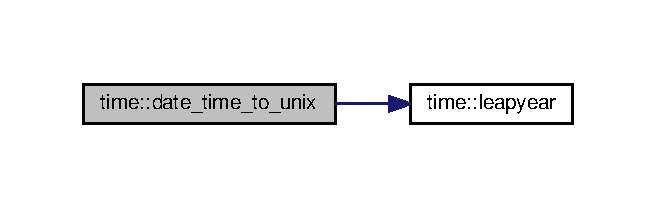
\includegraphics[width=315pt]{namespacetime_a7c66adfc707644b0644b33e1557f1486_cgraph}
\end{center}
\end{figure}


\index{time@{time}!days\+\_\+to\+\_\+date@{days\+\_\+to\+\_\+date}}
\index{days\+\_\+to\+\_\+date@{days\+\_\+to\+\_\+date}!time@{time}}
\subsubsection[{\texorpdfstring{days\+\_\+to\+\_\+date(\+S\+T\+Y\+E\+A\+R, S\+T\+M\+O\+N\+T\+H, S\+T\+D\+A\+Y, D\+A\+Y\+S, Y\+Y\+Y\+Y, M\+O, D\+D, H\+H, M\+M, S\+S)}{days_to_date(STYEAR, STMONTH, STDAY, DAYS, YYYY, MO, DD, HH, MM, SS)}}]{\setlength{\rightskip}{0pt plus 5cm}subroutine time\+::days\+\_\+to\+\_\+date (
\begin{DoxyParamCaption}
\item[{integer (kind=ik4), intent(in)}]{S\+T\+Y\+E\+AR, }
\item[{integer (kind=ik4), intent(in)}]{S\+T\+M\+O\+N\+TH, }
\item[{integer (kind=ik4), intent(in)}]{S\+T\+D\+AY, }
\item[{real (kind=rk8), dimension(\+:), intent(in)}]{D\+A\+YS, }
\item[{integer (kind=ik4), dimension(\+:), intent(out), optional}]{Y\+Y\+YY, }
\item[{integer (kind=ik4), dimension(\+:), intent(out), optional}]{MO, }
\item[{integer (kind=ik4), dimension(\+:), intent(out), optional}]{DD, }
\item[{integer (kind=ik4), dimension(\+:), intent(out), optional}]{HH, }
\item[{integer (kind=ik4), dimension(\+:), intent(out), optional}]{MM, }
\item[{integer (kind=ik4), dimension(\+:), intent(out), optional}]{SS}
\end{DoxyParamCaption}
)}\hypertarget{namespacetime_a29670e6cf798cee7d9e33201b38f9507}{}\label{namespacetime_a29670e6cf798cee7d9e33201b38f9507}


Definition at line 14 of file time.\+f90.


\begin{DoxyCode}
14 
15 \textcolor{keywordtype}{IMPLICIT NONE}
16 
17 \textcolor{keywordtype}{INTEGER (KIND=IK4)}, \textcolor{keywordtype}{INTENT(IN)}                          :: styear       \textcolor{comment}{! The year which the day count is
       relative to.}
18 \textcolor{keywordtype}{INTEGER (KIND=IK4)}, \textcolor{keywordtype}{INTENT(IN)}                          :: stmonth      \textcolor{comment}{! The month which the day count is
       relative to.}
19 \textcolor{keywordtype}{INTEGER (KIND=IK4)}, \textcolor{keywordtype}{INTENT(IN)}                          :: stday        \textcolor{comment}{! The day which the day count is
       relative to.}
20 \textcolor{keywordtype}{REAL (KIND=RK8)}, \textcolor{keywordtype}{DIMENSION(:)}, \textcolor{keywordtype}{INTENT(IN)}               :: days         \textcolor{comment}{! The time in days relative to
       STYEAR-STMONTH-STDAYT00:00:00}
21 \textcolor{keywordtype}{INTEGER (KIND=IK4)}, \textcolor{keywordtype}{DIMENSION(:)}, \textcolor{keywordtype}{INTENT(OUT)}, \textcolor{keywordtype}{OPTIONAL} :: yyyy         \textcolor{comment}{! The year.}
22 \textcolor{keywordtype}{INTEGER (KIND=IK4)}, \textcolor{keywordtype}{DIMENSION(:)}, \textcolor{keywordtype}{INTENT(OUT)}, \textcolor{keywordtype}{OPTIONAL} :: mo           \textcolor{comment}{! The month.}
23 \textcolor{keywordtype}{INTEGER (KIND=IK4)}, \textcolor{keywordtype}{DIMENSION(:)}, \textcolor{keywordtype}{INTENT(OUT)}, \textcolor{keywordtype}{OPTIONAL} :: dd           \textcolor{comment}{! The day.}
24 \textcolor{keywordtype}{INTEGER (KIND=IK4)}, \textcolor{keywordtype}{DIMENSION(:)}, \textcolor{keywordtype}{INTENT(OUT)}, \textcolor{keywordtype}{OPTIONAL} :: hh           \textcolor{comment}{! The hour.}
25 \textcolor{keywordtype}{INTEGER (KIND=IK4)}, \textcolor{keywordtype}{DIMENSION(:)}, \textcolor{keywordtype}{INTENT(OUT)}, \textcolor{keywordtype}{OPTIONAL} :: mm           \textcolor{comment}{! The minute.}
26 \textcolor{keywordtype}{INTEGER (KIND=IK4)}, \textcolor{keywordtype}{DIMENSION(:)}, \textcolor{keywordtype}{INTENT(OUT)}, \textcolor{keywordtype}{OPTIONAL} :: ss           \textcolor{comment}{! The second.}
27 
28 \textcolor{keywordtype}{INTEGER (KIND=IK4)}                                      :: nt           \textcolor{comment}{! Number of times in the time
       arrays.}
29 \textcolor{keywordtype}{INTEGER (KIND=IK4)}, \textcolor{keywordtype}{DIMENSION(12)}                       :: mdays    = (/31, 28, 31, 30, 31, 30, 31, 31, 30,
       31, 30, 31/)
30 \textcolor{keywordtype}{INTEGER (KIND=IK4)}                                      :: ii           \textcolor{comment}{! Counter.}
31 \textcolor{keywordtype}{REAL (KIND=RK8)}                                         :: tdn
32 \textcolor{keywordtype}{INTEGER (KIND=IK4)}                                      :: tyy, tmo, tdd, thh, tmm, tss, tti
33 
34 nt  = \textcolor{keyword}{SIZE}(days)
35 
36 \textcolor{keywordflow}{DO} ii=1,nt
37     tyy = styear
38     \textcolor{comment}{!}
39     \textcolor{comment}{! We do a bit of rounding stuff here, based on what outputs the user wants.}
40     \textcolor{comment}{!}
41     \textcolor{keywordflow}{IF} (\textcolor{keyword}{PRESENT}(ss)) \textcolor{keywordflow}{THEN}
42         tdn = int((days(ii)+(stday))*86400 + 0.5)/86400.      \textcolor{comment}{! Round to the nearest second.}
43     \textcolor{keywordflow}{ELSE} \textcolor{keywordflow}{IF} (\textcolor{keyword}{PRESENT}(mm)) \textcolor{keywordflow}{THEN}
44         tdn = int((days(ii)+(stday))*1440 + 0.5)/1440.        \textcolor{comment}{! Round to the nearest minute.}
45     \textcolor{keywordflow}{ELSE}
46         tdn = int((days(ii)+(stday))*24 + 0.5)/24.            \textcolor{comment}{! Round to the nearest hour.}
47 \textcolor{keywordflow}{    END IF}
48 
49     \textcolor{comment}{!}
50     \textcolor{comment}{! First calculate the date}
51     \textcolor{comment}{!}
52     tmo = stmonth
53     \textcolor{keywordflow}{DO} \textcolor{keywordflow}{WHILE} (tdn .GE. (mdays(tmo)+1))
54         \textcolor{keywordflow}{IF} (\hyperlink{namespacetime_ac7f82d40fd2b49e7e9025b103e88555c}{leapyear}(tyy)) \textcolor{keywordflow}{THEN}
55             mdays(2) = 29
56         \textcolor{keywordflow}{ELSE}
57             mdays(2) = 28
58 \textcolor{keywordflow}{        END IF}
59         \textcolor{keywordflow}{DO} \textcolor{keywordflow}{WHILE} ((tdn .GE. (mdays(tmo)+1)))
60             tdn = tdn - mdays(tmo)
61             tmo = tmo + 1
62             \textcolor{keywordflow}{if} (tmo > 12) \textcolor{keywordflow}{exit}
63 \textcolor{keywordflow}{        END DO}
64         \textcolor{keywordflow}{if} (tmo > 12) \textcolor{keywordflow}{then}
65             tyy = tyy + 1
66             tmo = 1
67 \textcolor{keywordflow}{       endif}
68 \textcolor{keywordflow}{    END DO}
69     tdd = int(tdn, kind=\hyperlink{namespaceportable_aa110cf333432508140602ea192c4b2ea}{ik4})
70     \textcolor{comment}{!}
71     \textcolor{comment}{! Now calculate the time, to the nearest second.}
72     \textcolor{comment}{!}
73     tti = int((tdn - tdd)*86400. + 0.5, kind=\hyperlink{namespaceportable_aa110cf333432508140602ea192c4b2ea}{ik4})     \textcolor{comment}{! Round to the nearest second.}
74     thh = tti/3600
75     tmm = (tti - thh*3600)/60
76     tss = tti - thh*3600 - tmm*60
77 
78     \textcolor{keywordflow}{IF} (\textcolor{keyword}{PRESENT}(yyyy))  yyyy(ii)    = tyy
79     \textcolor{keywordflow}{IF} (\textcolor{keyword}{PRESENT}(mo))    mo(ii)      = tmo
80     \textcolor{keywordflow}{IF} (\textcolor{keyword}{PRESENT}(dd))    dd(ii)      = tdd
81     \textcolor{keywordflow}{IF} (\textcolor{keyword}{PRESENT}(hh))    hh(ii)      = thh
82     \textcolor{keywordflow}{IF} (\textcolor{keyword}{PRESENT}(mm))    mm(ii)      = tmm
83     \textcolor{keywordflow}{IF} (\textcolor{keyword}{PRESENT}(ss))    ss(ii)      = tss
84 \textcolor{keywordflow}{END DO}
85     
86 
\end{DoxyCode}


Here is the call graph for this function\+:\nopagebreak
\begin{figure}[H]
\begin{center}
\leavevmode
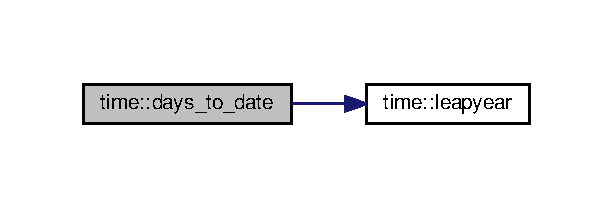
\includegraphics[width=294pt]{namespacetime_a29670e6cf798cee7d9e33201b38f9507_cgraph}
\end{center}
\end{figure}




Here is the caller graph for this function\+:\nopagebreak
\begin{figure}[H]
\begin{center}
\leavevmode
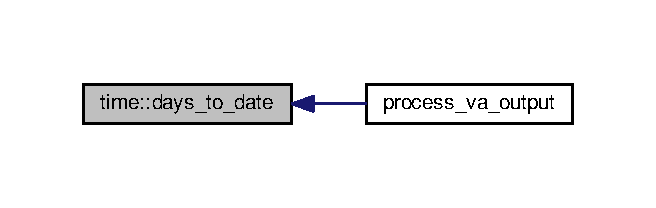
\includegraphics[width=315pt]{namespacetime_a29670e6cf798cee7d9e33201b38f9507_icgraph}
\end{center}
\end{figure}


\index{time@{time}!leapyear@{leapyear}}
\index{leapyear@{leapyear}!time@{time}}
\subsubsection[{\texorpdfstring{leapyear(\+Y\+E\+A\+R)}{leapyear(YEAR)}}]{\setlength{\rightskip}{0pt plus 5cm}logical function time\+::leapyear (
\begin{DoxyParamCaption}
\item[{integer (kind=ik4), intent(in)}]{Y\+E\+AR}
\end{DoxyParamCaption}
)}\hypertarget{namespacetime_ac7f82d40fd2b49e7e9025b103e88555c}{}\label{namespacetime_ac7f82d40fd2b49e7e9025b103e88555c}


Definition at line 220 of file time.\+f90.


\begin{DoxyCode}
220 
221 \textcolor{keywordtype}{IMPLICIT NONE}
222 \textcolor{keywordtype}{INTEGER (KIND=IK4)}, \textcolor{keywordtype}{INTENT(IN)}                          :: year         \textcolor{comment}{! The year being tested.}
223 
224 \textcolor{keywordflow}{IF} (mod(year,4) .EQ. 0) \textcolor{keywordflow}{THEN}
225     \textcolor{keywordflow}{IF} ((mod(year,100) .EQ. 0) .AND. (mod(year,400) .NE. 0)) \textcolor{keywordflow}{THEN}
226         \hyperlink{namespacetime_ac7f82d40fd2b49e7e9025b103e88555c}{leapyear}    = .false.
227     \textcolor{keywordflow}{ELSE}
228         \hyperlink{namespacetime_ac7f82d40fd2b49e7e9025b103e88555c}{leapyear}    = .true.
229 \textcolor{keywordflow}{    END IF}
230 \textcolor{keywordflow}{ELSE}
231     \hyperlink{namespacetime_ac7f82d40fd2b49e7e9025b103e88555c}{leapyear}        = .false.
232 \textcolor{keywordflow}{END IF}
233 
\end{DoxyCode}


Here is the caller graph for this function\+:\nopagebreak
\begin{figure}[H]
\begin{center}
\leavevmode
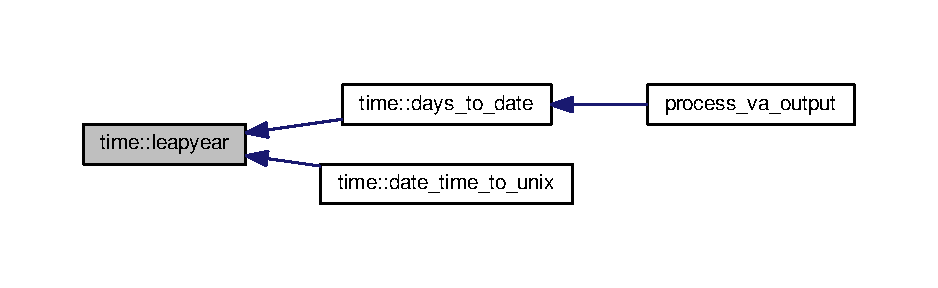
\includegraphics[width=350pt]{namespacetime_ac7f82d40fd2b49e7e9025b103e88555c_icgraph}
\end{center}
\end{figure}



\chapter{File Documentation}
\hypertarget{2d__put_8f90}{}\section{/home/unimelb.edu.\+au/mbergemann/va\+\_\+analysis/src/2d\+\_\+put.f90 File Reference}
\label{2d__put_8f90}\index{/home/unimelb.\+edu.\+au/mbergemann/va\+\_\+analysis/src/2d\+\_\+put.\+f90@{/home/unimelb.\+edu.\+au/mbergemann/va\+\_\+analysis/src/2d\+\_\+put.\+f90}}
\subsection*{Functions/\+Subroutines}
\begin{DoxyCompactItemize}
\item 
program \hyperlink{2d__put_8f90_af4920a0c6374e3dfdbc214dd992acbc7}{put\+\_\+2d}
\end{DoxyCompactItemize}


\subsection{Function/\+Subroutine Documentation}
\index{2d\+\_\+put.\+f90@{2d\+\_\+put.\+f90}!put\+\_\+2d@{put\+\_\+2d}}
\index{put\+\_\+2d@{put\+\_\+2d}!2d\+\_\+put.\+f90@{2d\+\_\+put.\+f90}}
\subsubsection[{\texorpdfstring{put\+\_\+2d}{put_2d}}]{\setlength{\rightskip}{0pt plus 5cm}program put\+\_\+2d (
\begin{DoxyParamCaption}
{}
\end{DoxyParamCaption}
)}\hypertarget{2d__put_8f90_af4920a0c6374e3dfdbc214dd992acbc7}{}\label{2d__put_8f90_af4920a0c6374e3dfdbc214dd992acbc7}


Definition at line 15 of file 2d\+\_\+put.\+f90.



Here is the call graph for this function\+:\nopagebreak
\begin{figure}[H]
\begin{center}
\leavevmode
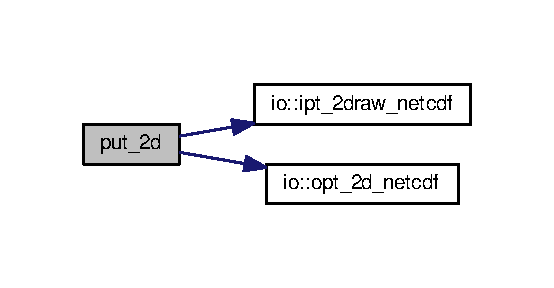
\includegraphics[width=266pt]{2d__put_8f90_af4920a0c6374e3dfdbc214dd992acbc7_cgraph}
\end{center}
\end{figure}



\hypertarget{3d__put_8f90}{}\section{/home/unimelb.edu.\+au/mbergemann/va\+\_\+analysis/src/3d\+\_\+put.f90 File Reference}
\label{3d__put_8f90}\index{/home/unimelb.\+edu.\+au/mbergemann/va\+\_\+analysis/src/3d\+\_\+put.\+f90@{/home/unimelb.\+edu.\+au/mbergemann/va\+\_\+analysis/src/3d\+\_\+put.\+f90}}
\subsection*{Functions/\+Subroutines}
\begin{DoxyCompactItemize}
\item 
program \hyperlink{3d__put_8f90_acf30b8d61a70feac6ec95b3b5803c1be}{put\+\_\+3d}
\end{DoxyCompactItemize}


\subsection{Function/\+Subroutine Documentation}
\index{3d\+\_\+put.\+f90@{3d\+\_\+put.\+f90}!put\+\_\+3d@{put\+\_\+3d}}
\index{put\+\_\+3d@{put\+\_\+3d}!3d\+\_\+put.\+f90@{3d\+\_\+put.\+f90}}
\subsubsection[{\texorpdfstring{put\+\_\+3d}{put_3d}}]{\setlength{\rightskip}{0pt plus 5cm}program put\+\_\+3d (
\begin{DoxyParamCaption}
{}
\end{DoxyParamCaption}
)}\hypertarget{3d__put_8f90_acf30b8d61a70feac6ec95b3b5803c1be}{}\label{3d__put_8f90_acf30b8d61a70feac6ec95b3b5803c1be}


Definition at line 10 of file 3d\+\_\+put.\+f90.



Here is the call graph for this function\+:\nopagebreak
\begin{figure}[H]
\begin{center}
\leavevmode
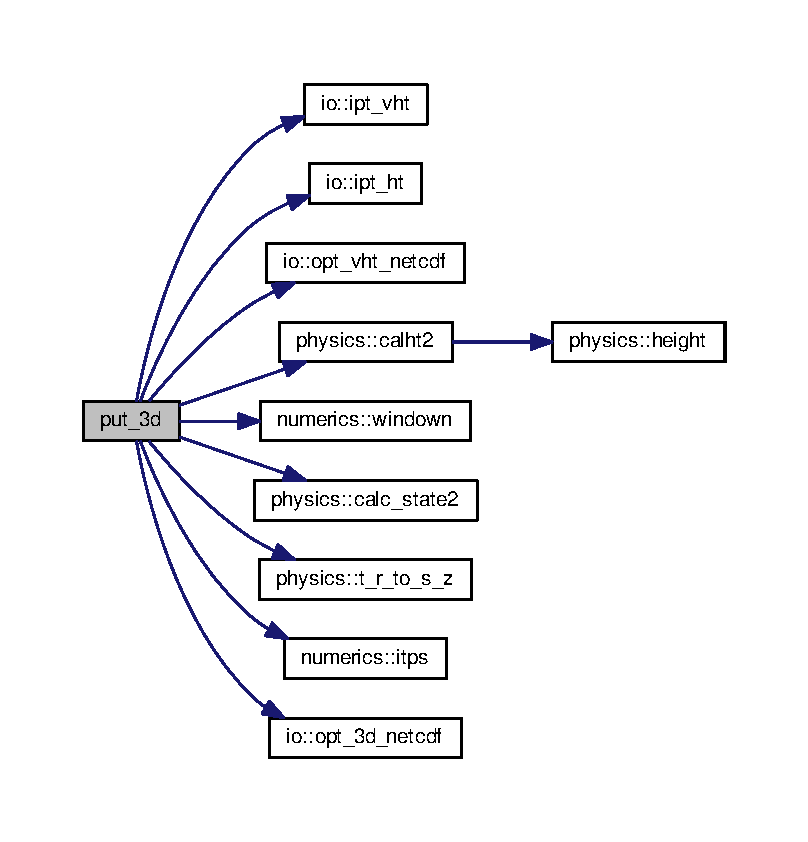
\includegraphics[width=350pt]{3d__put_8f90_acf30b8d61a70feac6ec95b3b5803c1be_cgraph}
\end{center}
\end{figure}



\hypertarget{budget__put_8f90}{}\section{/home/unimelb.edu.\+au/mbergemann/va\+\_\+analysis/src/budget\+\_\+put.f90 File Reference}
\label{budget__put_8f90}\index{/home/unimelb.\+edu.\+au/mbergemann/va\+\_\+analysis/src/budget\+\_\+put.\+f90@{/home/unimelb.\+edu.\+au/mbergemann/va\+\_\+analysis/src/budget\+\_\+put.\+f90}}
\subsection*{Functions/\+Subroutines}
\begin{DoxyCompactItemize}
\item 
program \hyperlink{budget__put_8f90_af79e3129f9674c9cd350ae2ba43e22f0}{budget\+\_\+put}
\end{DoxyCompactItemize}


\subsection{Function/\+Subroutine Documentation}
\index{budget\+\_\+put.\+f90@{budget\+\_\+put.\+f90}!budget\+\_\+put@{budget\+\_\+put}}
\index{budget\+\_\+put@{budget\+\_\+put}!budget\+\_\+put.\+f90@{budget\+\_\+put.\+f90}}
\subsubsection[{\texorpdfstring{budget\+\_\+put}{budget_put}}]{\setlength{\rightskip}{0pt plus 5cm}program budget\+\_\+put (
\begin{DoxyParamCaption}
{}
\end{DoxyParamCaption}
)}\hypertarget{budget__put_8f90_af79e3129f9674c9cd350ae2ba43e22f0}{}\label{budget__put_8f90_af79e3129f9674c9cd350ae2ba43e22f0}


Definition at line 10 of file budget\+\_\+put.\+f90.



Here is the call graph for this function\+:\nopagebreak
\begin{figure}[H]
\begin{center}
\leavevmode
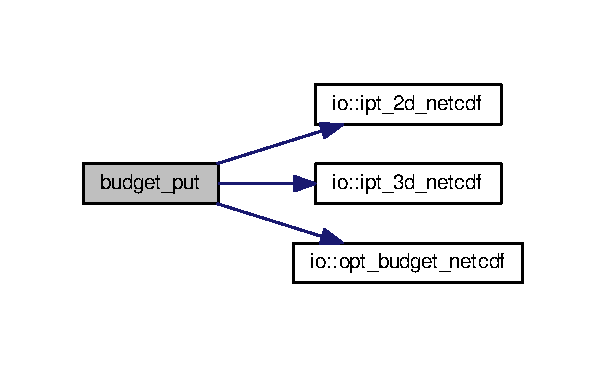
\includegraphics[width=291pt]{budget__put_8f90_af79e3129f9674c9cd350ae2ba43e22f0_cgraph}
\end{center}
\end{figure}



\hypertarget{constants_8f90}{}\section{/home/unimelb.edu.\+au/mbergemann/va\+\_\+analysis/src/constants.f90 File Reference}
\label{constants_8f90}\index{/home/unimelb.\+edu.\+au/mbergemann/va\+\_\+analysis/src/constants.\+f90@{/home/unimelb.\+edu.\+au/mbergemann/va\+\_\+analysis/src/constants.\+f90}}
\subsection*{Modules}
\begin{DoxyCompactItemize}
\item 
module \hyperlink{namespaceconstants}{constants}
\end{DoxyCompactItemize}
\subsection*{Variables}
\begin{DoxyCompactItemize}
\item 
real(kind=rk8), parameter \hyperlink{namespaceconstants_a064bd715409f723a4e6d45b6300c5ca0}{constants\+::pi} = 3.\+14159265
\item 
real(kind=rk8), parameter \hyperlink{namespaceconstants_afaa5eaa2c9ee648a808fb8e1c94e76f8}{constants\+::rearth} = 6371000
\item 
real(kind=rk8), parameter \hyperlink{namespaceconstants_a67051296d7b4bcd0d4cee08bba6e46fa}{constants\+::omega} = 7.\+292\+E-\/05
\item 
real(kind=rk8), parameter \hyperlink{namespaceconstants_ad91564da82b97ea0d29ce0565565db85}{constants\+::rd} = 287.\+04
\item 
real(kind=rk8), parameter \hyperlink{namespaceconstants_a7ef8fc37397fbfbefd3c22883378dcc5}{constants\+::rw} = 461.\+50
\item 
real(kind=rk8), parameter \hyperlink{namespaceconstants_a046aef138fbc8d05251d4fdc6eb3ee89}{constants\+::g} = 9.\+8
\item 
real(kind=rk8), parameter \hyperlink{namespaceconstants_afb3befdfd57058ee9d073b832134a601}{constants\+::lv0} = 2.\+5\+E6
\item 
real(kind=rk8), parameter \hyperlink{namespaceconstants_ab8db38b502faac0658c66b0d0b56c266}{constants\+::lv} = 2.\+501\+E6
\item 
real(kind=rk8), parameter \hyperlink{namespaceconstants_a0fdb1c80757efccb4c694c79206a3d83}{constants\+::ls} = 2.\+834\+E6
\item 
real(kind=rk8), parameter \hyperlink{namespaceconstants_abf3a57ecb3de0f79c3155c170db798f6}{constants\+::ls1} = 2.\+834\+E6
\item 
real(kind=rk8), parameter \hyperlink{namespaceconstants_a32354adf3493f59d0fc17b0302b2c368}{constants\+::cpd} = 1005.\+7
\item 
real(kind=rk8), parameter \hyperlink{namespaceconstants_afc5ea9cd5f9cf3a42e750ba5ab73c967}{constants\+::cpv} = 1870.\+0
\item 
real(kind=rk8), parameter \hyperlink{namespaceconstants_a4f2911e99beba65b9371b9a80d7c08d0}{constants\+::cl} = 4190.\+0
\item 
real(kind=rk8), parameter \hyperlink{namespaceconstants_a753fbbdd5d5b4af00d6819cb78ba99a1}{constants\+::t0} = 273.\+15
\item 
real(kind=rk8), parameter \hyperlink{namespaceconstants_a84ecaaf3771cbbfe65f7b15ef26bee36}{constants\+::cd} = 3.\+0\+E-\/3
\end{DoxyCompactItemize}

\hypertarget{io_8f90}{}\section{/home/unimelb.edu.\+au/mbergemann/va\+\_\+analysis/src/io.f90 File Reference}
\label{io_8f90}\index{/home/unimelb.\+edu.\+au/mbergemann/va\+\_\+analysis/src/io.\+f90@{/home/unimelb.\+edu.\+au/mbergemann/va\+\_\+analysis/src/io.\+f90}}
\subsection*{Modules}
\begin{DoxyCompactItemize}
\item 
module \hyperlink{namespaceio}{io}
\end{DoxyCompactItemize}
\subsection*{Functions/\+Subroutines}
\begin{DoxyCompactItemize}
\item 
subroutine \hyperlink{namespaceio_abed61f2af0a37265b7a1d15300f61996}{io\+::ipt\+\_\+vht} (I\+N\+P\+U\+T\+F\+I\+LE, I\+N\+S\+T\+R\+U\+M\+E\+NT, NV, NP, N\+ST, NT, V, P, ST, T, D)
\item 
subroutine \hyperlink{namespaceio_ae478b0148dea487c688bfea00e08cade}{io\+::ipt\+\_\+ht} (I\+N\+P\+U\+T\+F\+I\+LE, I\+N\+S\+T\+R\+U\+M\+E\+NT, NV, N\+ST, NT, V, ST, L\+ON, L\+AT, T, D)
\item 
subroutine \hyperlink{namespaceio_a1feb605e982e6696d29a63e635b8d3e1}{io\+::opt\+\_\+vht\+\_\+netcdf} (O\+U\+T\+P\+U\+T\+F\+I\+LE, I\+N\+S\+T\+R\+U\+M\+E\+NT, NV, NP, N\+ST, NT, V, P, ST, T, D)
\item 
subroutine \hyperlink{namespaceio_a63d1618c60598d1e5ac65348efb74bdc}{io\+::opt\+\_\+3d\+\_\+netcdf} (O\+U\+T\+P\+U\+T\+F\+I\+LE, DU, VU, DS, P, T, S\+TN, W\+E\+I\+G\+HT, B\+O\+U\+N\+D\+A\+RY, S\+T\+RU, S\+T\+RS)
\item 
subroutine \hyperlink{namespaceio_a0f9f8edb9a7173638e450ce3c4db7844}{io\+::ipt\+\_\+3d\+\_\+netcdf} (I\+N\+P\+U\+T\+F\+I\+LE, DU, VU, DS, T, S\+TN, W\+E\+I\+G\+HT, L\+EV, B\+O\+U\+N\+D\+A\+RY, S\+T\+RU, S\+T\+RS)
\item 
subroutine \hyperlink{namespaceio_ab1a423779bddf2d4557f39dd81431d93}{io\+::opt\+\_\+budget\+\_\+netcdf} (O\+U\+T\+P\+U\+T\+F\+I\+LE, B\+U\+D\+G\+E\+T\+\_\+\+C\+O\+L\+U\+MN, B\+U\+D\+G\+E\+T\+\_\+\+L\+A\+Y\+ER, V\+B\+U\+D\+G\+E\+T\+\_\+\+C\+O\+L\+U\+MN, V\+B\+U\+D\+G\+E\+T\+\_\+\+L\+A\+Y\+ER, A\+V\+E\+\_\+\+QS, A\+V\+E\+\_\+\+SS, P, T)
\item 
subroutine \hyperlink{namespaceio_aba707a842ac0a3e2e9def20af0b36c32}{io\+::ipt\+\_\+budget\+\_\+netcdf} (I\+N\+P\+U\+T\+F\+I\+LE, B\+U\+D\+G\+E\+T\+\_\+\+C\+O\+L\+U\+MN, B\+U\+D\+G\+E\+T\+\_\+\+L\+A\+Y\+ER, V\+B\+U\+D\+G\+E\+T\+\_\+\+C\+O\+L\+U\+MN, V\+B\+U\+D\+G\+E\+T\+\_\+\+L\+A\+Y\+ER, A\+V\+E\+\_\+\+QS, A\+V\+E\+\_\+\+SS, P, T)
\item 
subroutine \hyperlink{namespaceio_ab6bcb3dc7b4a08b242b7fbd4e11ed319}{io\+::opt\+\_\+2d\+\_\+netcdf} (O\+U\+T\+P\+U\+T\+F\+I\+LE, T, B\+A\+R\+\_\+\+P\+R\+ES, A\+D\+PS, P\+R\+E\+C\+IP, L\+P\+R\+E\+C\+IP, E\+V\+A\+P\+OR, S\+HF, RL, R\+A\+D\+I\+A\+T\+I\+O\+NT, R\+A\+D\+I\+A\+T\+I\+O\+NB, R\+A\+D\+I\+A\+T\+I\+ON, T\+A\+OX, T\+A\+OY)
\item 
subroutine \hyperlink{namespaceio_aff87bbb9c43d6db1fedd086586aab0c6}{io\+::ipt\+\_\+2d\+\_\+netcdf} (I\+N\+P\+U\+T\+F\+I\+LE, T, B\+A\+R\+\_\+\+P\+R\+ES, A\+D\+PS, P\+R\+E\+C\+IP, L\+P\+R\+E\+C\+IP, E\+V\+A\+P\+OR, S\+HF, RL, R\+A\+D\+I\+A\+T\+I\+O\+NT, R\+A\+D\+I\+A\+T\+I\+O\+NB, R\+A\+D\+I\+A\+T\+I\+ON, T\+A\+OX, T\+A\+OY)
\item 
subroutine \hyperlink{namespaceio_ac91ebbbf1426451d33f3e32b08f70aee}{io\+::ipt\+\_\+2draw\+\_\+netcdf} (I\+N\+P\+U\+T\+F\+I\+LE, V\+A\+R\+\_\+\+N\+A\+ME, V\+AR)
\item 
subroutine \hyperlink{namespaceio_a50ab1073758d8d341087a0755354011d}{io\+::opt\+\_\+forcing\+\_\+netcdf} (O\+U\+T\+P\+U\+T\+F\+I\+LE, S\+F\+C\+\_\+\+D\+A\+TA, M\+L\+\_\+\+D\+A\+TA, C\+F\+\_\+\+L\+ON, C\+F\+\_\+\+L\+AT, C\+F\+\_\+\+P\+H\+IS, P\+L\+E\+VS)
\end{DoxyCompactItemize}

\hypertarget{lu_8f90}{}\section{/home/unimelb.edu.\+au/mbergemann/va\+\_\+analysis/src/lu.f90 File Reference}
\label{lu_8f90}\index{/home/unimelb.\+edu.\+au/mbergemann/va\+\_\+analysis/src/lu.\+f90@{/home/unimelb.\+edu.\+au/mbergemann/va\+\_\+analysis/src/lu.\+f90}}
\subsection*{Modules}
\begin{DoxyCompactItemize}
\item 
module \hyperlink{namespacelu}{lu}
\end{DoxyCompactItemize}
\subsection*{Functions/\+Subroutines}
\begin{DoxyCompactItemize}
\item 
subroutine \hyperlink{namespacelu_a578a2275703e9c18d7f262f0a3482fbe}{lu\+::ludcmp} (A, N, I\+N\+DX, D, C\+O\+DE)
\item 
subroutine \hyperlink{namespacelu_a588ba20d76e8dd5c49b370d9ba3ec379}{lu\+::lubksb} (A, N, I\+N\+DX, B)
\end{DoxyCompactItemize}

\hypertarget{numerics_8f90}{}\section{/home/unimelb.edu.\+au/mbergemann/va\+\_\+analysis/src/numerics.f90 File Reference}
\label{numerics_8f90}\index{/home/unimelb.\+edu.\+au/mbergemann/va\+\_\+analysis/src/numerics.\+f90@{/home/unimelb.\+edu.\+au/mbergemann/va\+\_\+analysis/src/numerics.\+f90}}
\subsection*{Modules}
\begin{DoxyCompactItemize}
\item 
module \hyperlink{namespacenumerics}{numerics}
\end{DoxyCompactItemize}
\subsection*{Functions/\+Subroutines}
\begin{DoxyCompactItemize}
\item 
subroutine \hyperlink{namespacenumerics_ac972e0e69239cba641ad373fee101472}{numerics\+::itps} (KS, KB, D, DS)
\item 
subroutine \hyperlink{namespacenumerics_afbd04035bb50e63d44980bf39cf84ac3}{numerics\+::gmean} (MG, DP, NV, N\+ST, NT, T\+S\+M\+O\+O\+TH)
\item 
subroutine \hyperlink{namespacenumerics_a354d8c793bd1515de7af7cfa32c51389}{numerics\+::smooth} (A\+R\+R\+AY, N, F\+I\+L\+T\+E\+R\+\_\+\+W\+I\+D\+TH, C\+Y\+C\+L\+IC)
\item 
subroutine \hyperlink{namespacenumerics_add44a47f4f996c0266711b825fd6bb20}{numerics\+::caldev} (DU, KT, KS, N\+S\+TU, N\+TU, NP, N\+VU, D\+E\+V\+M2)
\item 
subroutine \hyperlink{namespacenumerics_a9581a41d0b81a5ded9690972e499c629}{numerics\+::horizontal\+\_\+field} (N\+ST, L\+ON, L\+AT, X, Y, F, D\+Z\+DX, D\+Z\+DY, D\+I\+VU, D\+I\+VV)
\item 
subroutine \hyperlink{namespacenumerics_a8e58d8bf1c738af1a91517fdb8b81aa2}{numerics\+::line\+\_\+fit\+\_\+xyz} (N, X, Y, Z, D\+Z\+DX, D\+Z\+DY, Z0)
\item 
subroutine \hyperlink{namespacenumerics_aa16b459eac85058fd1da1b9ebc4555b9}{numerics\+::windown} (N, X, DX, X1, L0, L1)
\item 
subroutine \hyperlink{namespacenumerics_acc1dd6ef9a4cf200fd7701143c4ae29e}{numerics\+::assim} (NP, DP, P, KS, KB, KT, N\+S\+TU, L\+O\+NU, L\+A\+TU, DU, N\+S\+TS, L\+O\+NS, L\+A\+TS, D\+SS, D\+I\+V\+B\+V\+AR, F\+CX, F\+CY, F\+PX, F\+PY, B\+U\+D\+G\+ET, N\+A\+D\+V\+AR, W\+V\+AR, D\+US)
\item 
subroutine \hyperlink{namespacenumerics_adbe2d748ef22c981cddde813d1db9d77}{numerics\+::calc\+\_\+budget\+\_\+layer} (NP, N\+TU, P, B\+U\+D\+G\+E\+T\+\_\+\+L\+A\+Y\+ER, B\+U\+D\+G\+E\+T\+\_\+\+C\+O\+L\+U\+M\+NS, A\+V\+E\+\_\+\+QS, A\+V\+E\+\_\+\+SS)
\end{DoxyCompactItemize}

\hypertarget{physics_8f90}{}\section{/home/unimelb.edu.\+au/mbergemann/va\+\_\+analysis/src/physics.f90 File Reference}
\label{physics_8f90}\index{/home/unimelb.\+edu.\+au/mbergemann/va\+\_\+analysis/src/physics.\+f90@{/home/unimelb.\+edu.\+au/mbergemann/va\+\_\+analysis/src/physics.\+f90}}
\subsection*{Modules}
\begin{DoxyCompactItemize}
\item 
module \hyperlink{namespacephysics}{physics}
\end{DoxyCompactItemize}
\subsection*{Functions/\+Subroutines}
\begin{DoxyCompactItemize}
\item 
subroutine \hyperlink{namespacephysics_a3f1959e7b3ff1a8d052f1e0441b1c379}{physics\+::s\+\_\+r\+\_\+to\+\_\+t\+\_\+z} (P, PS, ZS, S, R, T, Z)
\item 
subroutine \hyperlink{namespacephysics_aebc42cd426e3ef8e85696bb1c7da18c3}{physics\+::t\+\_\+r\+\_\+to\+\_\+s\+\_\+z} (P, PS, ZS, T, R, S, Z)
\item 
subroutine \hyperlink{namespacephysics_adc35216d512f6586071a79fba286a39c}{physics\+::diverg} (U\+N\+I\+TH, V\+AR, U, V, D\+I\+VU, D\+I\+VV, D\+I\+V1)
\item 
subroutine \hyperlink{namespacephysics_a56a179b5bd2c13a2201b2367037a42cf}{physics\+::fcorlx} (U\+N\+I\+TH, N\+S\+TU, F, V, F\+C\+X1)
\item 
subroutine \hyperlink{namespacephysics_a1f64bd544ea55c7fbbf5330725fc0896}{physics\+::fcorly} (U\+N\+I\+TH, N\+S\+TU, F, U, F\+C\+Y1)
\item 
subroutine \hyperlink{namespacephysics_acf841366af6f4fd7502b4031a2cacb56}{physics\+::fpgd} (U\+N\+I\+TH, Z, D\+Z\+DX, F\+P1)
\item 
subroutine \hyperlink{namespacephysics_a0ca41ce81224f2d7b292dc474c080c60}{physics\+::height} (NP, KS, KT, P, T, R, Z)
\item 
subroutine \hyperlink{namespacephysics_a16ab28545ccd5528dd72f50208761dbe}{physics\+::calht2} (PS, ZS, N, P, TC, R, HT, D\+EW)
\item 
subroutine \hyperlink{namespacephysics_a9197b79c7b8e6dfce5ecca360c320610}{physics\+::calc\+\_\+state2} (P, T, TD, E, Z, R, RH, H, H\+D\+RY, S)
\end{DoxyCompactItemize}

\hypertarget{portable_8f90}{}\section{/home/unimelb.edu.\+au/mbergemann/va\+\_\+analysis/src/portable.f90 File Reference}
\label{portable_8f90}\index{/home/unimelb.\+edu.\+au/mbergemann/va\+\_\+analysis/src/portable.\+f90@{/home/unimelb.\+edu.\+au/mbergemann/va\+\_\+analysis/src/portable.\+f90}}
\subsection*{Modules}
\begin{DoxyCompactItemize}
\item 
module \hyperlink{namespaceportable}{portable}
\end{DoxyCompactItemize}
\subsection*{Variables}
\begin{DoxyCompactItemize}
\item 
integer, parameter \hyperlink{namespaceportable_aaeaca599bf9baead529cbb42680f0f0b}{portable\+::ik1} = S\+E\+L\+E\+C\+T\+E\+D\+\_\+\+I\+N\+T\+\_\+\+K\+I\+ND(2)
\item 
integer, parameter \hyperlink{namespaceportable_a35a0fbff20f9df8a8a5de95c97dc7d5d}{portable\+::ik2} = S\+E\+L\+E\+C\+T\+E\+D\+\_\+\+I\+N\+T\+\_\+\+K\+I\+ND(4)
\item 
integer, parameter \hyperlink{namespaceportable_aa110cf333432508140602ea192c4b2ea}{portable\+::ik4} = S\+E\+L\+E\+C\+T\+E\+D\+\_\+\+I\+N\+T\+\_\+\+K\+I\+ND(9)
\item 
integer, parameter \hyperlink{namespaceportable_abaed22a509442771d3fba69bebda0b33}{portable\+::rk4} = S\+E\+L\+E\+C\+T\+E\+D\+\_\+\+R\+E\+A\+L\+\_\+\+K\+I\+ND(4, 30)
\item 
integer, parameter \hyperlink{namespaceportable_a609d4b38b4f128b310e288b1861ad9bd}{portable\+::rk8} = S\+E\+L\+E\+C\+T\+E\+D\+\_\+\+R\+E\+A\+L\+\_\+\+K\+I\+ND(10, 200)
\end{DoxyCompactItemize}

\hypertarget{process__va__output_8f90}{}\section{/home/unimelb.edu.\+au/mbergemann/va\+\_\+analysis/src/process\+\_\+va\+\_\+output.f90 File Reference}
\label{process__va__output_8f90}\index{/home/unimelb.\+edu.\+au/mbergemann/va\+\_\+analysis/src/process\+\_\+va\+\_\+output.\+f90@{/home/unimelb.\+edu.\+au/mbergemann/va\+\_\+analysis/src/process\+\_\+va\+\_\+output.\+f90}}
\subsection*{Functions/\+Subroutines}
\begin{DoxyCompactItemize}
\item 
program \hyperlink{process__va__output_8f90_a05600ca128b4d3cb32091909ace2e376}{process\+\_\+va\+\_\+output}
\end{DoxyCompactItemize}


\subsection{Function/\+Subroutine Documentation}
\index{process\+\_\+va\+\_\+output.\+f90@{process\+\_\+va\+\_\+output.\+f90}!process\+\_\+va\+\_\+output@{process\+\_\+va\+\_\+output}}
\index{process\+\_\+va\+\_\+output@{process\+\_\+va\+\_\+output}!process\+\_\+va\+\_\+output.\+f90@{process\+\_\+va\+\_\+output.\+f90}}
\subsubsection[{\texorpdfstring{process\+\_\+va\+\_\+output}{process_va_output}}]{\setlength{\rightskip}{0pt plus 5cm}program process\+\_\+va\+\_\+output (
\begin{DoxyParamCaption}
{}
\end{DoxyParamCaption}
)}\hypertarget{process__va__output_8f90_a05600ca128b4d3cb32091909ace2e376}{}\label{process__va__output_8f90_a05600ca128b4d3cb32091909ace2e376}


Definition at line 9 of file process\+\_\+va\+\_\+output.\+f90.



Here is the call graph for this function\+:\nopagebreak
\begin{figure}[H]
\begin{center}
\leavevmode
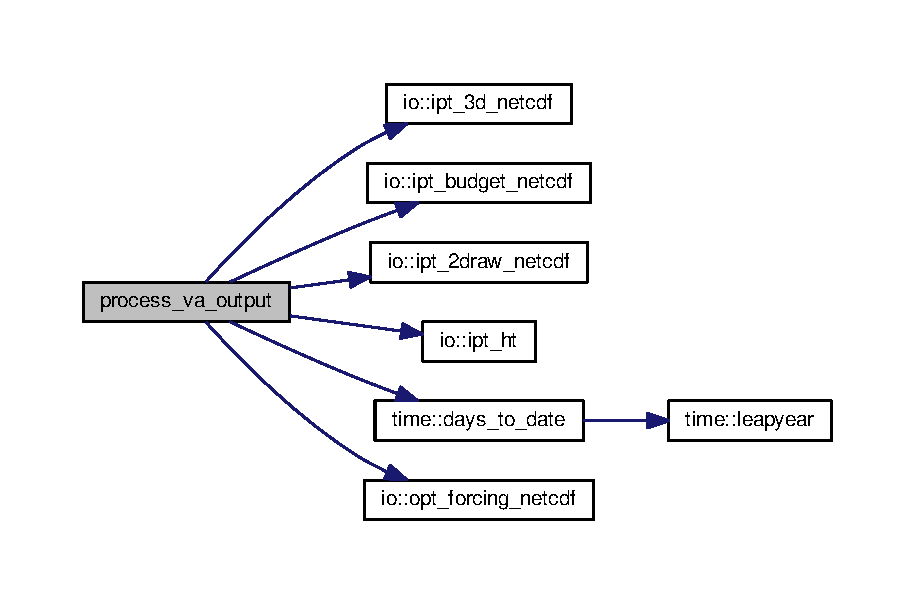
\includegraphics[width=350pt]{process__va__output_8f90_a05600ca128b4d3cb32091909ace2e376_cgraph}
\end{center}
\end{figure}



\hypertarget{settings_8f90}{}\section{/home/unimelb.edu.\+au/mbergemann/va\+\_\+analysis/src/settings.f90 File Reference}
\label{settings_8f90}\index{/home/unimelb.\+edu.\+au/mbergemann/va\+\_\+analysis/src/settings.\+f90@{/home/unimelb.\+edu.\+au/mbergemann/va\+\_\+analysis/src/settings.\+f90}}
\subsection*{Modules}
\begin{DoxyCompactItemize}
\item 
module \hyperlink{namespacesettings}{settings}
\end{DoxyCompactItemize}
\subsection*{Variables}
\begin{DoxyCompactItemize}
\item 
real(kind=rk8), parameter \hyperlink{namespacesettings_a80b5ece3c388ad5e0c924f372afebe65}{settings\+::pstart} =200.\+0
\item 
real(kind=rk8), parameter \hyperlink{namespacesettings_a8d5e7d0c921e46fc4b2c7d7738729805}{settings\+::pcrit} =200.\+0
\item 
integer(kind=ik4), parameter \hyperlink{namespacesettings_a78876a80ce867f4bc71866b783b6de89}{settings\+::nvbudget\+\_\+column} =5
\item 
integer(kind=ik4), parameter \hyperlink{namespacesettings_a42675226258d1641f557f9e8e756b76e}{settings\+::nvbudget\+\_\+layer} =6
\item 
integer(kind=ik4), parameter \hyperlink{namespacesettings_a3e7f9f832f20c3352f6a1c901bf3d13b}{settings\+::ntermmax} =7
\item 
integer(kind=ik4), parameter \hyperlink{namespacesettings_acb91032130faf4bb56bee66af8cbf573}{settings\+::ntermmaxv} =8
\item 
integer(kind=ik4), parameter \hyperlink{namespacesettings_a4f624be133b88a44c8976b47b85e8eec}{settings\+::nad} =3
\item 
integer(kind=ik4), parameter \hyperlink{namespacesettings_a45f66b2df6e7509477bcf669702044a8}{settings\+::nstx0} =10
\item 
integer(kind=ik4), parameter \hyperlink{namespacesettings_a3989615b44f5121ea2e8761d6abc24e1}{settings\+::nsty0} =9
\item 
integer(kind=ik4), parameter \hyperlink{namespacesettings_a79e2ff19d589b215ed9176906dd5cbbf}{settings\+::nvu} =10
\item 
integer(kind=ik4), parameter \hyperlink{namespacesettings_ac10106479d8b3db1c5edd195b8dbf36e}{settings\+::nvs} = N\+VU
\item 
real(kind=rk8), parameter \hyperlink{namespacesettings_ac94cc887999dc993bb580baf0ce85ce3}{settings\+::pt} =90.\+0
\item 
integer(kind=ik4), parameter \hyperlink{namespacesettings_a6feb18d2b9a31062fd7bc3f5533b0a4f}{settings\+::start\+\_\+year} =2004
\item 
integer(kind=ik4), parameter \hyperlink{namespacesettings_a10988f9d662713f7f29e611c9b6c873d}{settings\+::start\+\_\+month} =10
\item 
integer(kind=ik4), parameter \hyperlink{namespacesettings_a9d8f79c61533111bb5efd5ee1577108f}{settings\+::start\+\_\+day} = 1
\end{DoxyCompactItemize}

\hypertarget{setup_8py}{}\section{/home/unimelb.edu.\+au/mbergemann/va\+\_\+analysis/src/setup.py File Reference}
\label{setup_8py}\index{/home/unimelb.\+edu.\+au/mbergemann/va\+\_\+analysis/src/setup.\+py@{/home/unimelb.\+edu.\+au/mbergemann/va\+\_\+analysis/src/setup.\+py}}
\subsection*{Namespaces}
\begin{DoxyCompactItemize}
\item 
 \hyperlink{namespacesetup}{setup}
\end{DoxyCompactItemize}
\subsection*{Functions}
\begin{DoxyCompactItemize}
\item 
def \hyperlink{namespacesetup_a98c11c98a822ccbe47d135174bfcc346}{setup.\+file\+\_\+search} (file)
\item 
def \hyperlink{namespacesetup_a3477c4ce4216a75efaf147946c414f4f}{setup.\+checkenv} (var, alt)
\end{DoxyCompactItemize}
\subsection*{Variables}
\begin{DoxyCompactItemize}
\item 
\hyperlink{namespacesetup_ad8426f1e8d88dc4a6601f003805f9224}{setup.\+Os} = platform.\+system()
\item 
\hyperlink{namespacesetup_a26e74581e39df55b9dbba8dcf7d485fe}{setup.\+host} = socket.\+gethostname().lower()
\item 
float \hyperlink{namespacesetup_aea013977d24d48e57270f412b2c222c2}{setup.\+sleep} = 0.\+2
\item 
string \hyperlink{namespacesetup_a299d8d9205ed54eac073b608d9ab6af8}{setup.\+Path} = \textquotesingle{}/opt/local\textquotesingle{}
\item 
bool \hyperlink{namespacesetup_a5dd2d263367c323cbd4d063b156a4a68}{setup.\+help} = True
\item 
string \hyperlink{namespacesetup_a2429357b780b7445dd4831250478d9ed}{setup.\+txt}
\item 
\hyperlink{namespacesetup_aaadd587ba3f34c400f5df2cf05a7e1c5}{setup.\+altnames} = dict(sed=\textquotesingle{}sed\textquotesingle{},awk=\textquotesingle{}awk\textquotesingle{},date=\textquotesingle{}date\textquotesingle{})
\item 
\hyperlink{namespacesetup_ac2fa2127d48feb1a28f2aafa6fd00d0b}{setup.\+L\+D\+F\+L\+A\+GS} = L\+D\+F\+L\+A\+G\+S.\+split(\textquotesingle{},\textquotesingle{})
\item 
list \hyperlink{namespacesetup_a82d52368b879302df365513569195970}{setup.\+missing\+\_\+package} = \mbox{[}$\,$\mbox{]}
\item 
tuple \hyperlink{namespacesetup_a38fd627eae7d93f3366e9b4f707e77dd}{setup.\+checkbin}
\item 
\hyperlink{namespacesetup_ab82b87b5daf568d1c5c3c8fc41e52ca1}{setup.\+status} = False
\item 
\hyperlink{namespacesetup_a501d41aa25b2969d3234702d4439c931}{setup.\+fn}
\item 
list \hyperlink{namespacesetup_a9c08eb458bd1b35c49b4aeddb58b03af}{setup.\+missing\+\_\+module} = \mbox{[}$\,$\mbox{]}
\item 
\hyperlink{namespacesetup_ada820daab4af8948c6a81a2bc70ec3e8}{setup.\+method} = dict(pbs=\textquotesingle{}qsub\textquotesingle{},slurm=\textquotesingle{}sbatch\textquotesingle{})\mbox{[}B\+A\+T\+CH\mbox{]}
\item 
\hyperlink{namespacesetup_a5c8a4998256b5c6d0700ac432fa75d4b}{setup.\+B\+A\+T\+CH} = B\+A\+T\+C\+H.\+lower()
\item 
\hyperlink{namespacesetup_aac6afb4198c065254f41a7ce8297da6a}{setup.\+proj\+\_\+file} = os.\+path.\+join(os.\+pardir,\textquotesingle{}.proj\textquotesingle{})
\item 
\hyperlink{namespacesetup_ac86422d915b07533937fc858abea97a4}{setup.\+a} = raw\+\_\+input(\textquotesingle{}Warning option for creating batch jobs is set but no P\+R\+O\+J\+E\+CT if given, is that correct? \mbox{[}Y$\vert$n\mbox{]}\+: \textquotesingle{})
\item 
\hyperlink{namespacesetup_aea6945a959274b18887b0be79239ead7}{setup.\+f} = open(proj\+\_\+file,\textquotesingle{}w\textquotesingle{})
\item 
\hyperlink{namespacesetup_a4046afba70953007c6ba74e7d9c6bd5f}{setup.\+M\+A\+IL} = raw\+\_\+input(\textquotesingle{}No user email is given, enter now\+: \textquotesingle{})
\item 
string \hyperlink{namespacesetup_accce39b4aa713fbb290144ec68f888af}{setup.\+batch\+\_\+header} = u\char`\"{}\char`\"{}
\item 
string \hyperlink{namespacesetup_a86918b8c879471590485d8ac229362b2}{setup.\+batch\+\_\+job}
\item 
\hyperlink{namespacesetup_a2331c56366b88428b33ad78c625cfcc8}{setup.\+bash\+\_\+script} = os.\+path.\+join(os.\+pardir,\textquotesingle{}submit\+\_\+\%s.\+sh\textquotesingle{}\%B\+A\+T\+CH)
\item 
list \hyperlink{namespacesetup_a29c6bb44f4b88076bbd129b6114c9fd2}{setup.\+version\+\_\+conflict} = \mbox{[}$\,$\mbox{]}
\item 
\hyperlink{namespacesetup_a27ac718b5c714e7f887a5769bb81e54e}{setup.\+cmd} = altnames\mbox{[}command\mbox{]}
\item 
\hyperlink{namespacesetup_a46c1652bf2b2336d1bf166fc69cbb168}{setup.\+process} = Popen(\mbox{[}cmd,\textquotesingle{}-\/-\/version\textquotesingle{}\mbox{]},stdout=P\+I\+PE)
\item 
\hyperlink{namespacesetup_a9a9fe68847ae604c87e0c586206415d9}{setup.\+output}
\item 
\hyperlink{namespacesetup_ad9eccefc3ae62bb9f91bbbfa97900e49}{setup.\+err}
\item 
\hyperlink{namespacesetup_a7e4d34412eadfa1481215bd61b81d64d}{setup.\+exit\+\_\+code} = process.\+wait()
\item 
\hyperlink{namespacesetup_a8ebf34a9903eb2abbfbd92f17e3b89a4}{setup.\+fl} = float(\textquotesingle{}.\textquotesingle{}.join(re.\+findall(r\textquotesingle{}\textbackslash{}d+\textquotesingle{},output.\+split(\textquotesingle{}\textbackslash{}n\textquotesingle{})\mbox{[}0\mbox{]})\mbox{[}0\+:2\mbox{]}))
\item 
string \hyperlink{namespacesetup_a11da39b62ca84bc7e300d60f43bf46a8}{setup.\+makefile\+\_\+var}
\item 
string \hyperlink{namespacesetup_acdec383554bf7f66e8fe06336ebfca98}{setup.\+makefile\+\_\+radar}
\end{DoxyCompactItemize}

\hypertarget{time_8f90}{}\section{/home/unimelb.edu.\+au/mbergemann/va\+\_\+analysis/src/time.f90 File Reference}
\label{time_8f90}\index{/home/unimelb.\+edu.\+au/mbergemann/va\+\_\+analysis/src/time.\+f90@{/home/unimelb.\+edu.\+au/mbergemann/va\+\_\+analysis/src/time.\+f90}}
\subsection*{Modules}
\begin{DoxyCompactItemize}
\item 
module \hyperlink{namespacetime}{time}
\end{DoxyCompactItemize}
\subsection*{Functions/\+Subroutines}
\begin{DoxyCompactItemize}
\item 
subroutine \hyperlink{namespacetime_a29670e6cf798cee7d9e33201b38f9507}{time\+::days\+\_\+to\+\_\+date} (S\+T\+Y\+E\+AR, S\+T\+M\+O\+N\+TH, S\+T\+D\+AY, D\+A\+YS, Y\+Y\+YY, MO, DD, HH, MM, SS)
\item 
integer(kind=ik4) function \hyperlink{namespacetime_a7c66adfc707644b0644b33e1557f1486}{time\+::date\+\_\+time\+\_\+to\+\_\+unix} (Y\+Y\+YY, MO, DD, HH, MM, SS)
\item 
logical function \hyperlink{namespacetime_ac7f82d40fd2b49e7e9025b103e88555c}{time\+::leapyear} (Y\+E\+AR)
\end{DoxyCompactItemize}

\hypertarget{variational__analysis_8f90}{}\section{/home/unimelb.edu.\+au/mbergemann/va\+\_\+analysis/src/variational\+\_\+analysis.f90 File Reference}
\label{variational__analysis_8f90}\index{/home/unimelb.\+edu.\+au/mbergemann/va\+\_\+analysis/src/variational\+\_\+analysis.\+f90@{/home/unimelb.\+edu.\+au/mbergemann/va\+\_\+analysis/src/variational\+\_\+analysis.\+f90}}
\subsection*{Functions/\+Subroutines}
\begin{DoxyCompactItemize}
\item 
program \hyperlink{variational__analysis_8f90_a0f4a4c6f0c078ae2f3474734189851ca}{variational\+\_\+analysis}
\end{DoxyCompactItemize}


\subsection{Function/\+Subroutine Documentation}
\index{variational\+\_\+analysis.\+f90@{variational\+\_\+analysis.\+f90}!variational\+\_\+analysis@{variational\+\_\+analysis}}
\index{variational\+\_\+analysis@{variational\+\_\+analysis}!variational\+\_\+analysis.\+f90@{variational\+\_\+analysis.\+f90}}
\subsubsection[{\texorpdfstring{variational\+\_\+analysis}{variational_analysis}}]{\setlength{\rightskip}{0pt plus 5cm}program variational\+\_\+analysis (
\begin{DoxyParamCaption}
{}
\end{DoxyParamCaption}
)}\hypertarget{variational__analysis_8f90_a0f4a4c6f0c078ae2f3474734189851ca}{}\label{variational__analysis_8f90_a0f4a4c6f0c078ae2f3474734189851ca}


Definition at line 18 of file variational\+\_\+analysis.\+f90.



Here is the call graph for this function\+:\nopagebreak
\begin{figure}[H]
\begin{center}
\leavevmode
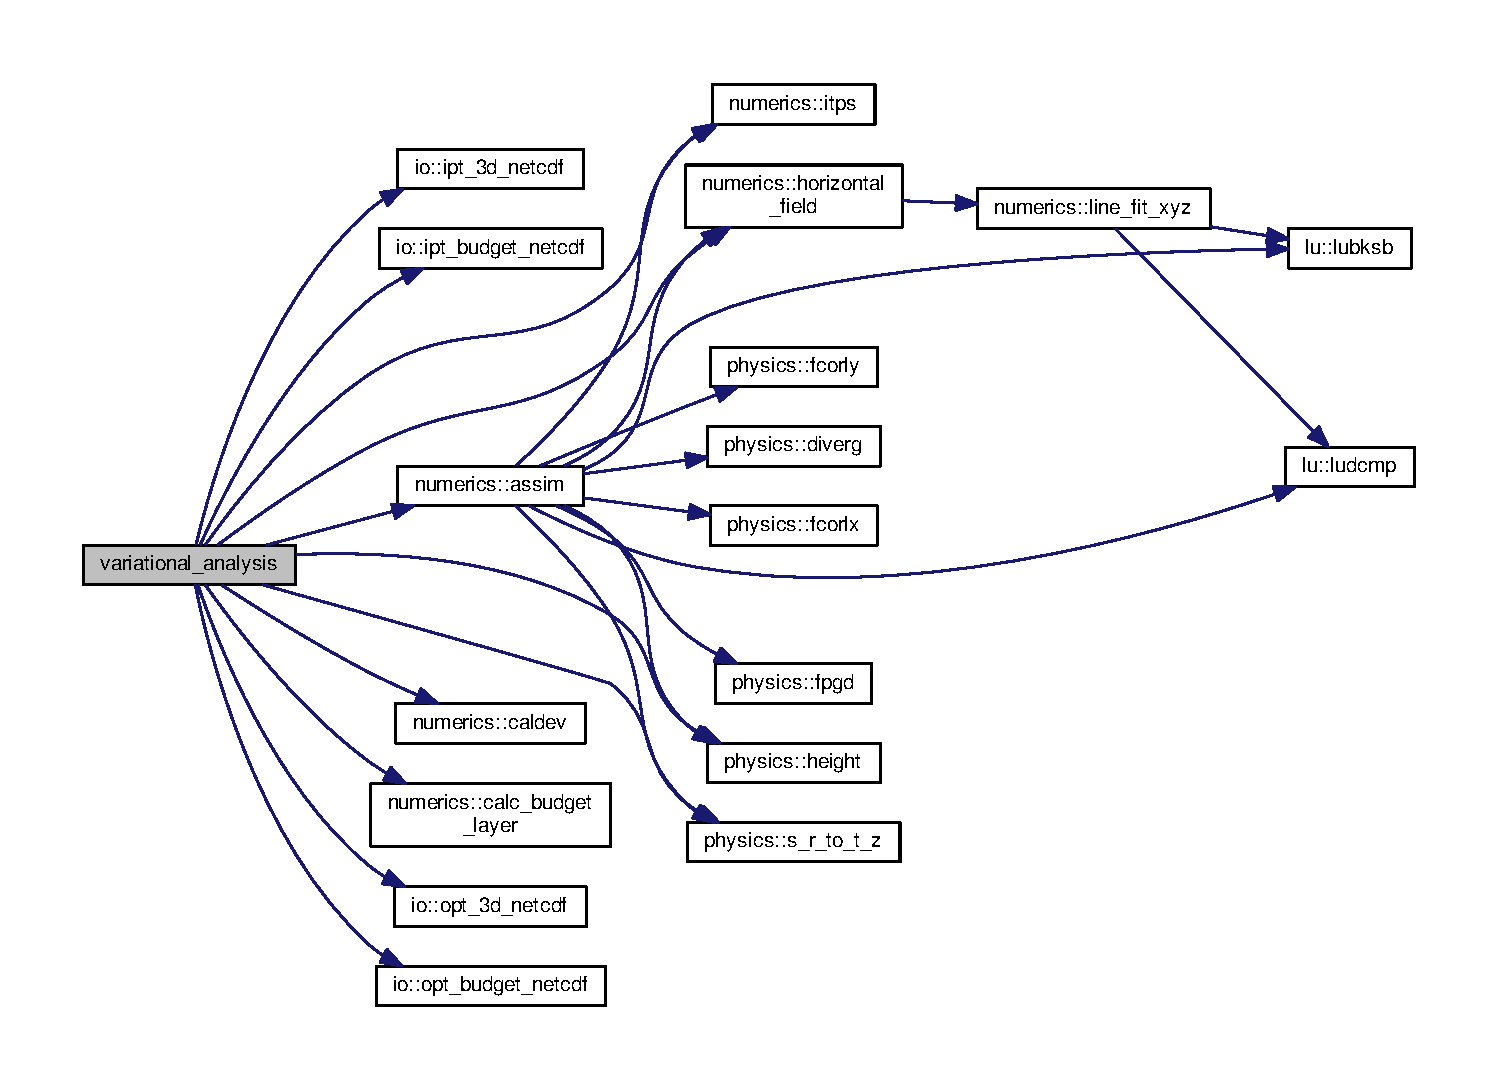
\includegraphics[width=350pt]{variational__analysis_8f90_a0f4a4c6f0c078ae2f3474734189851ca_cgraph}
\end{center}
\end{figure}



%--- End generated contents ---

% Index
\backmatter
\newpage
\phantomsection
\clearemptydoublepage
\addcontentsline{toc}{chapter}{Index}
\printindex

\end{document}
